% UCL Thesis LaTeX Template
%  (c) Ian Kirker, 2014
% 
% This is a template/skeleton for PhD/MPhil/MRes theses.
%
% It uses a rather split-up file structure because this tends to
%  work well for large, complex documents.
% We suggest using one file per chapter, but you may wish to use more
%  or fewer separate files than that.
% We've also separated out various bits of configuration into their
%  own files, to keep everything neat.
% Note that the \input command just streams in whatever file you give
%  it, while the \include command adds a page break, and does some
%  extra organisation to make compilation faster. Note that you can't
%  use \include inside an \include-d file.
% We suggest using \input for settings and configuration files that
%  you always want to use, and \include for each section of content.
% If you do that, it also means you can use the \includeonly statement
%  to only compile up the section you're currently interested in.
% You might also want to put figures into their own files to be \input.

% For more information on \input and \include, see:
%  http://tex.stackexchange.com/questions/246/when-should-i-use-input-vs-include


% Formatting and binding rules for theses are here: 
%  https://www.ucl.ac.uk/students/exams-and-assessments/research-assessments/format-bind-and-submit-your-thesis-general-guidance

% This package goes first and foremost, because it checks all 
%  your syntax for mistakes and some old-fashioned LaTeX commands.
% Note that normally you should load your documentclass before 
%  packages, because some packages change behaviour based on
%  your document settings.
% Also, for those confused by the RequirePackage here vs usepackage
%  elsewhere, usepackage cannot be used before the documentclass
%  command, while RequirePackage can. That's the only functional
%  difference as far as I'm aware.
\RequirePackage[l2tabu, orthodox]{nag}


% ------ Main document class specification ------
% The draft option here prevents images being inserted,
%  and adds chunky black bars to boxes that are exceeding 
%  the page width (to show that they are).
% The oneside option can optionally be replaced by twoside if
%  you intend to print double-sided. Note that this is
%  *specifically permitted* by the UCL thesis formatting
%  guidelines.
%
% Valid options in terms of type are:
%  phd
%  mres
%  mphil
%\documentclass[12pt,phd,draft,a4paper,oneside]{ucl_thesis}
\documentclass[12pt,phd,final,a4paper,oneside]{ucl_thesis}


% Package configuration:
%  LaTeX uses "packages" to add extra commands and features.
%  There are quite a few useful ones, so we've put them in a 
%   separate file.
% -------- Packages --------

% This package just gives you a quick way to dump in some sample text.
% You can remove it -- it's just here for the examples.
\usepackage{blindtext}

% This package means empty pages (pages with no text) won't get stuff
%  like chapter names at the top of the page. It's mostly cosmetic.
\usepackage{emptypage}

% The graphicx package adds the \includegraphics command,
%  which is your basic command for adding a picture.
\usepackage{graphicx}

% The float package improves LaTeX's handling of floats,
%  and also adds the option to *force* LaTeX to put the float
%  HERE, with the [H] option to the float environment.
\usepackage{float}

% The amsmath package enhances the various ways of including
%  maths, including adding the align environment for aligned
%  equations.
\usepackage{amsmath}

% Use these two packages together -- they define symbols
%  for e.g. units that you can use in both text and math mode.
\usepackage{gensymb}
\usepackage{textcomp}
% You may also want the units package for making little
%  fractions for unit specifications.
%\usepackage{units}


% The setspace package lets you use 1.5-sized or double line spacing.
\usepackage{setspace}
\setstretch{1.5}

% That just does body text -- if you want to expand *everything*,
%  including footnotes and tables, use this instead:
%\renewcommand{\baselinestretch}{1.5}


% PGFPlots is either a really clunky or really good way to add graphs
%  into your document, depending on your point of view.
% There's waaaaay too much information on using this to cover here,
%  so, you might want to start here:
%   http://pgfplots.sourceforge.net/
%  or here:
%   http://pgfplots.sourceforge.net/pgfplots.pdf
%\usepackage{pgfplots}
%\pgfplotsset{compat=1.3} % <- this fixed axis labels in the version I was using

% PGFPlotsTable can help you make tables a little more easily than
%  usual in LaTeX.
% If you're going to have to paste data in a lot, I'd suggest using it.
%  You might want to start with the manual, here:
%  http://pgfplots.sourceforge.net/pgfplotstable.pdf
%\usepackage{pgfplotstable}

% These settings are also recommended for using with pgfplotstable.
%\pgfplotstableset{
%	% these columns/<colname>/.style={<options>} things define a style
%	% which applies to <colname> only.
%	empty cells with={--}, % replace empty cells with '--'
%	every head row/.style={before row=\toprule,after row=\midrule},
%	every last row/.style={after row=\bottomrule}
%}


% The mhchem package provides chemistry formula typesetting commands
%  e.g. \ce{H2O}
%\usepackage[version=3]{mhchem}

% And the chemfig package gives a weird command for adding Lewis 
%  diagrams, for e.g. organic molecules
%\usepackage{chemfig}

% The linenumbers command from the lineno package adds line numbers
%  alongside your text that can be useful for discussing edits 
%  in drafts.
% Remove or comment out the command for proper versions.
%\usepackage[modulo]{lineno}
% \linenumbers 


% Alternatively, you can use the ifdraft package to let you add
%  commands that will only be used in draft versions
%\usepackage{ifdraft}

% For example, the following adds a watermark if the draft mode is on.
%\ifdraft{
%  \usepackage{draftwatermark}
%  \SetWatermarkText{\shortstack{\textsc{Draft Mode}\\ \strut \\ \strut \\ \strut}}
%  \SetWatermarkScale{0.5}
%  \SetWatermarkAngle{90}
%}


% The multirow package adds the option to make cells span 
%  rows in tables.
\usepackage{multirow}


% Subfig allows you to create figures within figures, to, for example,
%  make a single figure with 4 individually labeled and referenceable
%  sub-figures.
% It's quite fiddly to use, so check the documentation.
%\usepackage{subfig}

% The natbib package allows book-type citations commonly used in
%  longer works, and less commonly in science articles (IME).
% e.g. (Saucer et al., 1993) rather than [1]
% More details are here: http://merkel.zoneo.net/Latex/natbib.php
%\usepackage{natbib}

% The bibentry package (along with the \nobibliography* command)
%  allows putting full reference lines inline.
%  See: 
%   http://tex.stackexchange.com/questions/2905/how-can-i-list-references-from-bibtex-file-in-line-with-commentary
\usepackage{bibentry}

% The isorot package allows you to put things sideways 
%  (or indeed, at any angle) on a page.
% This can be useful for wide graphs or other figures.
%\usepackage{isorot}

% The caption package adds more options for caption formatting.
% This set-up makes hanging labels, makes the caption text smaller
%  than the body text, and makes the label bold.
% Highly recommended.
\usepackage[format=hang,font=small,labelfont=bf]{caption}

% If you're getting into defining your own commands, you might want
%  to check out the etoolbox package -- it defines a few commands
%  that can make it easier to make commands robust.
\usepackage{etoolbox}
\usepackage[inkscapeversion=1]{svg}
\usepackage{booktabs}
\usepackage{algorithm}
\usepackage[noend]{algpseudocode}
\usepackage{minted}
\usemintedstyle{tango}
%\usemintedstyle{bw}
\renewcommand{\theFancyVerbLine}{\sffamily{\footnotesize\arabic{FancyVerbLine}:}}
\usepackage{har2nat}
\usepackage{fancyhdr}
\setcitestyle{citesep={;}, aysep={,}}
\usepackage{graphicx}
\usepackage{subcaption}
\usepackage{wrapfig}
\usepackage[autostyle]{csquotes}
% just for using the warning sign
\usepackage{fontawesome}
% to insert verbatim environment that can change font size
\usepackage{fancyvrb}
% to get size of current font
\usepackage{relsize}
\graphicspath{ {fig/} }
\svgpath{{fig/}}

% Sets up links within your document, for e.g. contents page entries
%  and references, and also PDF metadata.
% You should edit this!
\input{LinksAndMetadata}

% And then some settings in separate files.
\input{FloatSettings} % For things like figures and tables
\bibliographystyle{agsm}   % For bibliographies

% These control how many number sections your subsections will take
%    e.g. Section 2.3.1.5.6.3
%  and how many of those will get put into the contents pages.
\setcounter{secnumdepth}{3}
\setcounter{tocdepth}{3}

% Ensure Helvetica
\renewcommand\familydefault{\sfdefault}

\begin{document}

%\nobibliography*
% ^-- This is a dumb trick that works with the bibentry package to let
%  you put bibliography entries whereever you like.
% I used this to put references to papers a chapter's work was 
%  published in at the end of that chapter.
% For more information, see: http://stefaanlippens.net/bibentry

% If you haven't finished making your full BibTex file yet, you
%  might find this useful -- it'll just replace all your
%  citations with little superscript notes.
% Uncomment to use.
%\renewcommand{\cite}[1]{\emph{\textsuperscript{[#1]}}}

% At last, content! Remember filenames are case-sensitive and 
%  *must not* include spaces.
% I may change the way this is done in a future version, 
%  but given that some people needed it, if you need a different degree title 
%  (e.g. Master of Science, Master in Science, Master of Arts, etc)
%  uncomment the following 3 lines and set as appropriate (this *has* to be before \maketitle)
\makeatletter
\renewcommand {\@degree@string} {Master of Science}
\makeatother
% Set course title, comment out to go back to default "University College london"
\makeatletter
\renewcommand {\@course@title} {Architectural Computation}
\makeatother
% Change course title preposition, comment out to go back to default "of"
\makeatletter
\renewcommand {\@course@title@preposition} {in}
\makeatother

% Flags for content selection; 
% They should be before calls to \maketitle, \makedeclaration etc.
% If set to true, download EPS file from: https://imagestore.ucl.ac.uk/imagestore/start/ucl-banners/For%20PRINT?authrequest=1&https=1
\setbool{useuclbanner}{true}
\uclbannerlocation{fig/banner.png}

\title{BARC0141: Built Environment Dissertation}
\subtit{Evaluating Office Layout Effects on Evacuation Time Using Social Force Model}
\author{Robin Song}
\department{The Bartlett School of Architecture}

% You can use this for extra information after the boilerplate declaration.
% Use the \\ macro for new lines. Can be useful if you have to declare
% contributions on papers.
\extradeclaration{}

\maketitle

\begin{abstract} % 300 word limit

With the development of modern office spaces towards higher density, the efficiency of emergency evacuation has become a key factor in ensuring life safety. Existing research mostly focuses on the simulation accuracy of pedestrian models or the independent influence of single parameters, while systematic studies on the variable geometric layout parameters within office spaces and their coupling effects are still insufficient. Therefore, this study systematically explores how internal spatial parameters, such as furniture layout, corridor and door width, and the number of exits, affects evacuation efficiency. The study adopts an agent-based modeling approach and conducts simulation experiments on two office prototypes of different scales in a parametric workflow integrating Rhino and JuPedSim, using the social force model. Quantitative evaluations are made through indicators such as total evacuation time (TET) and congestion hotspots. The research finds that internal layout parameters have a significant nonlinear impact on evacuation efficiency: increasing the width of corridors or exits shows a clear "diminishing marginal benefit" effect; at the same time, there is a strong coupling effect among parameters. When downstream channels are narrow, blindly widening the doors of upstream rooms will instead aggravate congestion and prolong evacuation time. The research conclusion confirms that the internal geometric configuration of office spaces is a key factor affecting evacuation efficiency, and its optimization requires a comprehensive consideration of the thresholds and coupling relationships among parameters, rather than maximizing a single parameter. This study provides parametric design basis for architects, and future research can validate the simulation with real data and consider more dynamic factors.

\textbf{Key Words:} Emergency evacuation, office layout, agent-based modeling, social force model, pedestrian dynamics, parametric design.

\end{abstract}

% \begin{impactstatement}

%     UCL theses now have to include an impact statement. \textit{(I think for REF reasons?)} The following text is the description from the guide linked from the formatting and submission website of what that involves. (Link to the guide: {\scriptsize \url{http://www.grad.ucl.ac.uk/essinfo/docs/Impact-Statement-Guidance-Notes-for-Research-Students-and-Supervisors.pdf}})

%     \begin{quote}
%         The statement should describe, in no more than 500 words, how the expertise, knowledge, analysis,
%         discovery or insight presented in your thesis could be put to a beneficial use. Consider benefits both
%         inside and outside academia and the ways in which these benefits could be brought about.

%         The benefits inside academia could be to the discipline and future scholarship, research methods or
%         methodology, the curriculum; they might be within your research area and potentially within other
%         research areas.

%         The benefits outside academia could occur to commercial activity, social enterprise, professional
%         practice, clinical use, public health, public policy design, public service delivery, laws, public
%         discourse, culture, the quality of the environment or quality of life.

%         The impact could occur locally, regionally, nationally or internationally, to individuals, communities or
%         organisations and could be immediate or occur incrementally, in the context of a broader field of
%         research, over many years, decades or longer.

%         Impact could be brought about through disseminating outputs (either in scholarly journals or
%         elsewhere such as specialist or mainstream media), education, public engagement, translational
%         research, commercial and social enterprise activity, engaging with public policy makers and public
%         service delivery practitioners, influencing ministers, collaborating with academics and non-academics
%         etc.

%         Further information including a searchable list of hundreds of examples of UCL impact outside of
%         academia please see \url{https://www.ucl.ac.uk/impact/}. For thousands more examples, please see
%         \url{http://results.ref.ac.uk/Results/SelectUoa}.
%     \end{quote}
% \end{impactstatement}

% \begin{acknowledgements}
%     First of all, I would like to express my most sincere gratitude to my supervisor, Petros Koutsolampros. From the conception of the topic to the final completion of the thesis, he has always provided me with insightful guidance and valuable suggestions. His rigorous academic attitude and profound professional knowledge helped me overcome many challenges in the research. At the same time, I would also like to thank my technical supervisor, Sherif Tarabishy, who gave me crucial and valuable advice when I was setting up the workflow between Rhino and JuPedSim, which was essential for the technical realization of this research. 

%     I also sincerely want to thank my family and my girlfriend. During my master's studies, they have always been my strongest support. Their understanding and support have been the foundation for me to focus on my studies without any distractions.
% \end{acknowledgements}

\setcounter{tocdepth}{2}
% Setting this higher means you get contents entries for
%  more minor section headers.

\tableofcontents
% \listoffigures
% \listoftables
% \renewcommand\listoflistingscaption{List of source codes}
% \listoflistings


\chapter{Introduction}
\label{introChapter}
As office space density continues to increase, emergency evacuation efficiency has become a key determining factor for personnel safety. Although research in the fields of crowd dynamics and evacuation simulation is quite extensive \cite{gwynneReviewMethodologiesUsed1999}, most of them focuses on the simulation accuracy of pedestrian models and the impact analysis of isolated parameters. There is still a lack of research on architectural space layout and multi-factor coupling effects.

Therefore this study aims to systematically explore the impact of internal spatial geometric configuration parameters (such as table layout, corridor width, number of exits and door width, etc.) on the efficiency of evacuation of a office space. 

The research will focus on the following questions: 
\begin{itemize}
    \item How does the layout of furnitures affect evacuation efficiency and path formation?
    \item What is the marginal effect of corridor width and exit parameters on evacuation dynamics and the regulatory role of congestion patterns?
    \item How would the gate width before exit influence the formation of the path?
    \item What is the relationship between the evacuation time distribution and the path distribution under different gate width configurations?
\end{itemize}

Through the simulation of two scale office prototypes, we can examine how these internal layout parameters systematically regulate the evacuation process, in order to provide data-driven optimization suggestions for the safety design of office.

\chapter{Literature Review}
\label{literatureReviewChapter}
\section{JuPedSim}
JuPedSim (Julich Pedestrian Simulator) is an open-source software framework for pedestrian dynamics and personnel evacuation simulation, aiming to study the movement and evacuation behaviors of people in the built environment through computer simulation. This tool takes "self-driven multi-agent system" as its core concept, modeling each pedestrian as an independent agent. The agents follow a set of rules in a given scene to determine their own movement path, speed and interaction behavior, thereby presenting phenomena such as flow, congestion, queuing and path selection at the group level at the macro level. JuPedSim is often coupled with microscopic simulation models such as the classic Social Force Model. By setting parameters such as the input geometric scene, entrance/exit conditions, channel width, and density, a quantitative evaluation of the evacuation performance in a specific scene can be obtained.

\section{Social Force Model}
In simulations of emergency evacuation scenarios, researchers usually employ modeling methods such as social force models, cellular automata as well as agent-based models to simulate the complexity of crowd behavior. These models have become the primary approach in this field of study.
The social force model is an appealing method because it offers a relatively open and scalable framework. Compared to other models, the social force model can more intuitively explain the interactions between individuals and can replicate complex phenomena in crowded environments, such as speed, density and queuing situations. This model was first introduced by Helbing and Molnár in 1995 \cite{helbingSocialForceModel1995}, attempting to accurately simulate crowd behavior from a microscopic dynamics perspective, analogous to gas dynamics. Its core idea is to view crowd movement as a dynamic process influenced by various "forces".
Many researchers have continuously improved and applied the social force model, further expanding its potential. For example, Zheng and others combined the social force model with neural networks to simulate collective behavior in different scenarios; Seyfried and colleagues made modifications to pedestrian dynamics for qualitative analysis; Parisi and Dorso utilized this model to study the evacuation process in rooms with exits. These studies indicate that the social force model has become an important tool for simulating crowd movement, showing broad application prospects especially in areas like traffic planning and architectural design.

\section{Rhino and Grasshopper}
The study's modeling and simulation workflow are conducted in Rhino 9 WIP, using Rhino as the geometry and initial agents placement environment. Grasshopper serves as the parametric front-end to drive the simulations, passing geometric inputs (polylines, doors, corridors, etc.) as point lists to the agent-based simulation instance.
Grasshopper is extended via Python scripting to enable seamless integration with JuPedSim. A Python 3.13 environment is used to write the bridge scripts that map Rhino/Grasshopper geometry to JuPedSim input scenes and to extract trajectories, speeds, congestion metrics, and other diagnostics from JuPedSim outputs for downstream analysis. We didn't use Rhino before version 9 WIP because it is the first version that supports Python 3.13(Rhino 8's Python is 3.9), which is required by JuPedSim.

\section{Previous Work}
An important branch of evacuation simulation is the research on physical environmental factors. The key elements of spatial structure include the geometric form of buildings, exit configuration and the distribution of obstacles. The geometric form of buildings involves the shape of rooms, floor height and corridor width, and these parameters directly affect the possibility and efficiency of crowd movement. Exit configuration, including the number, location and width of exits, is a key factor in determining the evacuation speed. In addition, the distribution of obstacles, such as the spatial positions of fixed facilities like tables, chairs and columns, significantly affects the evacuation paths and crowd speeds .

In 2012, Ma et al. conducted experimental research on evacuation in China's skycrappers, focusing on the impact of building physical characteristics on the evacuation process. Peacock and Kuligowski (2004) systematically reviewed occupant movement in buildings and found that physical environment factors, including space configuration, exit placement, and obstacle distribution, significantly affect evacuation efficiency. Koo et al. (2013) compared evacuation strategies in high-rise buildings, particularly examining the paths of disabled individuals under different physical conditions. Their study revealed that the geometry and design of exits directly determine the feasibility and safety of evacuations. In high-density and emergency situations, these physical factors can greatly influence crowd behavior during evacuations. A common conclusion from these studies is that the physical environment is a significant influence on evacuation simulation, necessitating a comprehensive consideration of building shape, exit quantity and location, stair width, and obstacle distribution.

In research on classrooms and office spaces, while exit design is important, an increasing number of studies highlight the significant impact of internal furniture arrangement, desk layout, and corner configurations on evacuation efficiency. In some situations, these internal layout factors can outweigh the influence of exit width or quantity (Liu, Parhizgar, 2018;). Helbing et al. specifically emphasized the considerable effect of obstacles, such as desks in a classroom, on evacuation efficiency. These findings indicate that optimizing layout by adjusting internal environmental parameters can significantly alter crowd path choices and congestion hotspots.

\section{Research Gap}
Despite the extensive research on evacuation simulations, there is still a lack of systematic exploration of how internal layout parameters affect evacuation performance in fixed structural settings. 

Firstly, existing studies lack a systematic analysis of how internal layout parameters interact. Most of the studies only focus on single parameter such as number of exits and layout of desks and seats, while ignoring factors including corners, corridor width and door width as well as their interaction, particularly in senarios with multiple exits and neted rooms.

Secondly, there is a lack of research on prototypes with different sizes. The lack of reliable methods for scaling from small and simple spaces to large and complex layout limits the translation of research results into practical applications.

Third, current research primarily focuses on simple scenarios such as classrooms, while systematic studies on the layout of office spaces are relatively scarce. Unlike traditional scenarios like classrooms, office spaces exhibit a high degree of complexity, including densely populated crowds, diverse furniture configurations, and dynamic layouts. The uniqueness of office spaces lies in the relatively fixed initial positions of personnel and the significant flexibility of furniture arrangements. Therefore, changes in the layout of office spaces may significantly impact evacuation efficiency, making them an ideal subject for evacuation simulation research.

Based on the aforementioned research limitations, the innovation of this study lies in: under the fixed structural constraints of office space scenarios, systematically comparing the evacuation performance of different scales and multiple layout variants, and revealing the coupling effects of door width, corridor width, and exit configuration through quantitative analysis. This research not only provides an actionable method for assessing the safety of office spaces but also offers a new methodological perspective for evacuation simulation studies.
%%%%%%

\chapter{Methedology}
\label{methodologyChapter}
\section{System integration and technology stack}

\subsection{Objectives and Framework }
This research achieved parametric coupling of Rhino 9's Grasshopper with JuPedSim, using Grasshopper to represent office floor geometry (polylines as point lists) and initial agent positions(points). A Python script will call JuPedSim's API to map the geometry from Rhino to the input for the JuPedSim scene, utilizing a social force model for microscopic simulations within Rhino. 
\subsection{Technology Stack and Versions}
Rhino 9 (Grasshopper) + Python (3.13, meeting JuPedSim's compatibility requirements);
\\JuPedSim (Julich Pedestrian Simulator) and its Social Force Model; 
\\Data analysis and processing: JupyterLab + Python (Pandas, NumPy, Matplotlib/Seaborn, SQLAlchemy/sqlite3); 
\\Data storage and playback: Each simulation outputs an SQLite database file for offline playback and statistical analysis. 
\subsection{Input and Output Description }
Input: Office geometry (polylines representing contours, doors, corridors, etc.), initial agent positions (Grasshopper point sets), and scene parameters (island table layout, corridor width, number of exits, door widths, etc.). 
\\Output: Each simulation round outputs the raw trajectory data as a SQLite file, while derived metrics such as speeds, congestion events, and other diagnostics are computed from these trajectories for subsequent analysis. Metadata (version, environment, random seed, etc.) are recorded as part of the analysis workflow.
\begin{figure}[h]
    \centering
    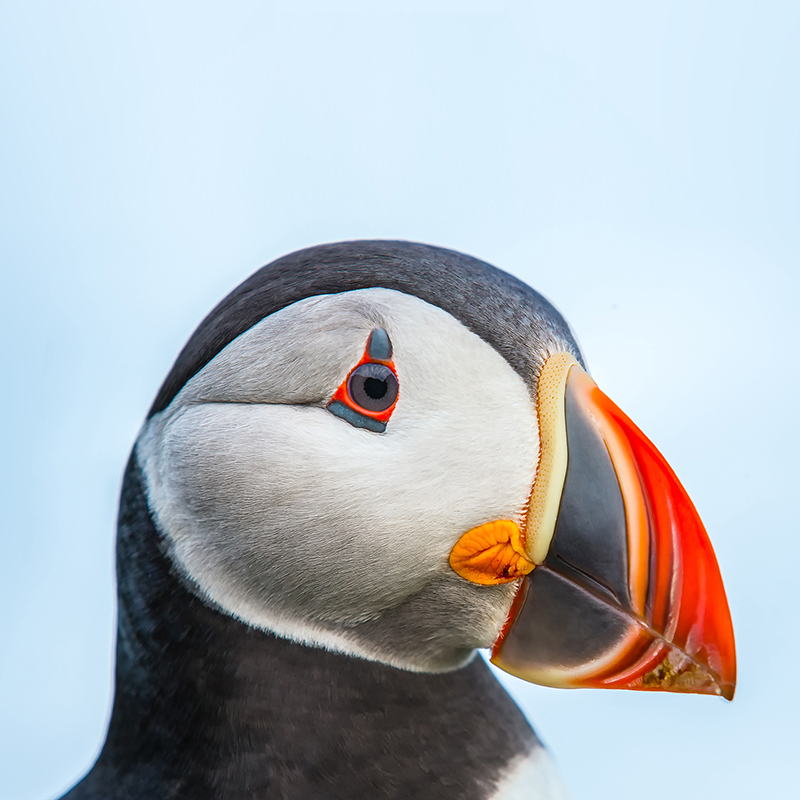
\includegraphics[width=\textwidth]{puffin}
    \caption{Data Pipeline}
    \label{fig:pipeline}
\end{figure}

\section{Experimental design}

\subsection{Prototype Scales}
Small prototype \ref{fig:small}: Focus on the preliminary effects of layout on evacuation paths and times, with rapid iteration through smaller geometric dimensions. To eliminate the influence of multiple corridors, we extended the bottom wall to the leftmost and bottommost sides, keeping only the Main corridor while controlling its width.
\begin{figure}[h]
    \centering
    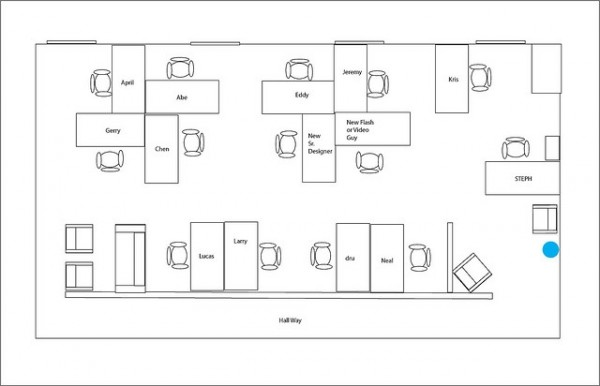
\includegraphics[width=\textwidth]{Small.jpg}
    \caption{Small Prototype}
    \label{fig:small}
\end{figure}
\\Big prototype \ref{fig:big}: Introduce higher-level issues such as door width coupling and multi-room nesting, testing the coupling effects at scales closer to actual office spaces.
\begin{figure}[h]
    \centering
    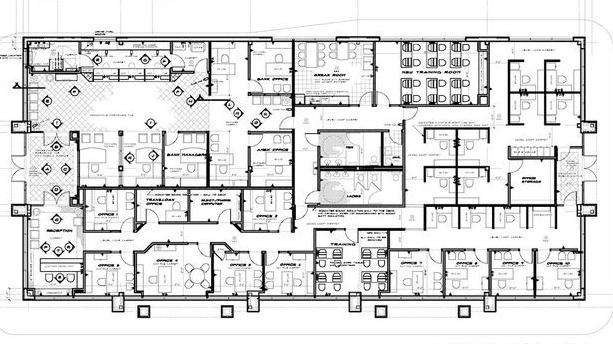
\includegraphics[width=\textwidth]{Big.jpg}
    \caption{Big Prototype}
    \label{fig:big}
\end{figure}

\subsection{Randomness and Replication}
Each parameter configuration is repeated 5 times, with initial positions randomly sampled from a Grasshopper point set to reduce the impact of randomness on the results.

\subsection{Small Prototype Variables}
Island Table Layout \ref{fig:abc}: Three variants A, B, and C represent the internal furniture configuration's representative parameters.
\begin{figure}[h]
    \centering
    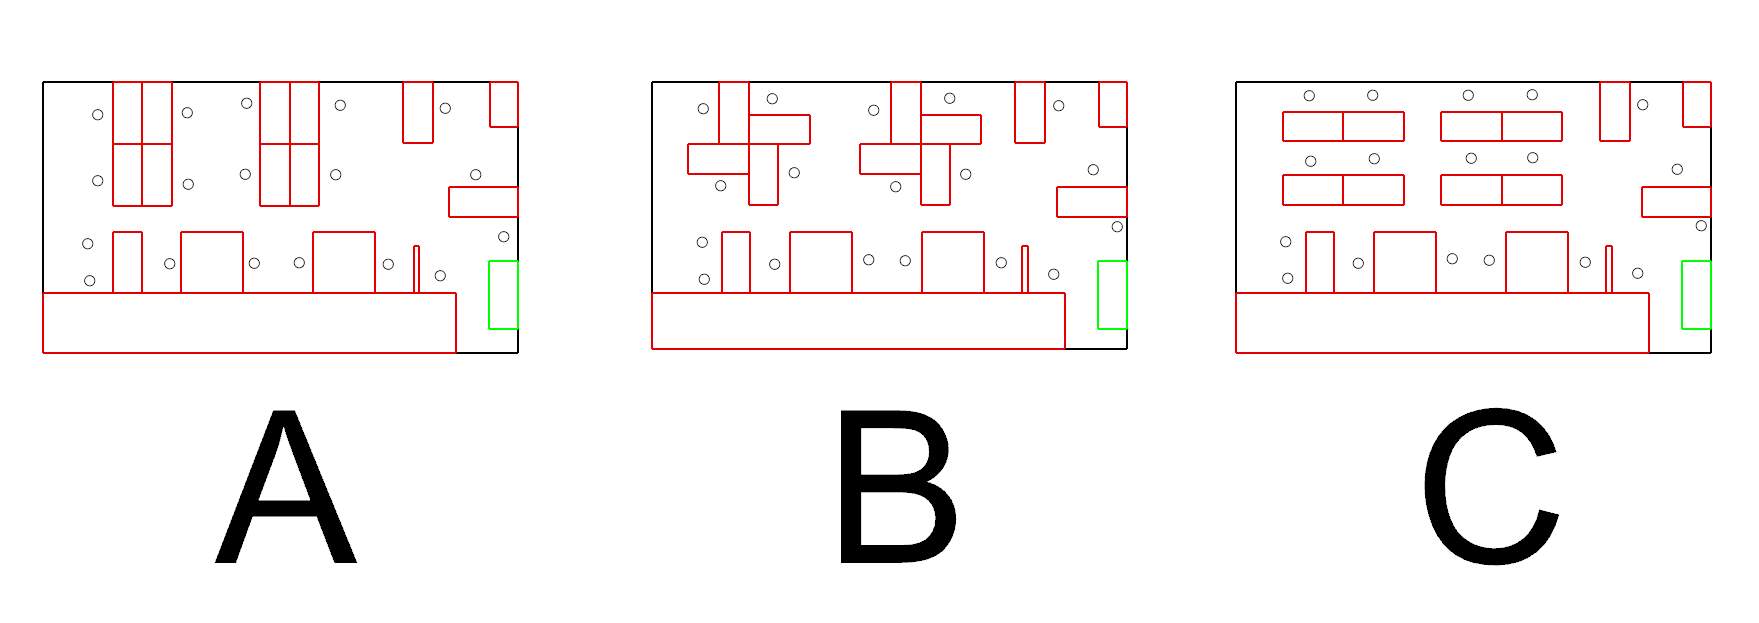
\includegraphics[width=\textwidth]{abc.png}
    \caption{Island Table Layout}
    \label{fig:abc}
\end{figure}

Corridor Width \ref{fig:corridorwidth}: 0.8 m,1.0m, 1.2 m, 1.4m, 1.6 m, 1.8m, 2.0 m, 2.2m, 2.4 m to explore the sensitivity of corridor width on path formation and congestion.
\begin{figure}[h]
    \centering
    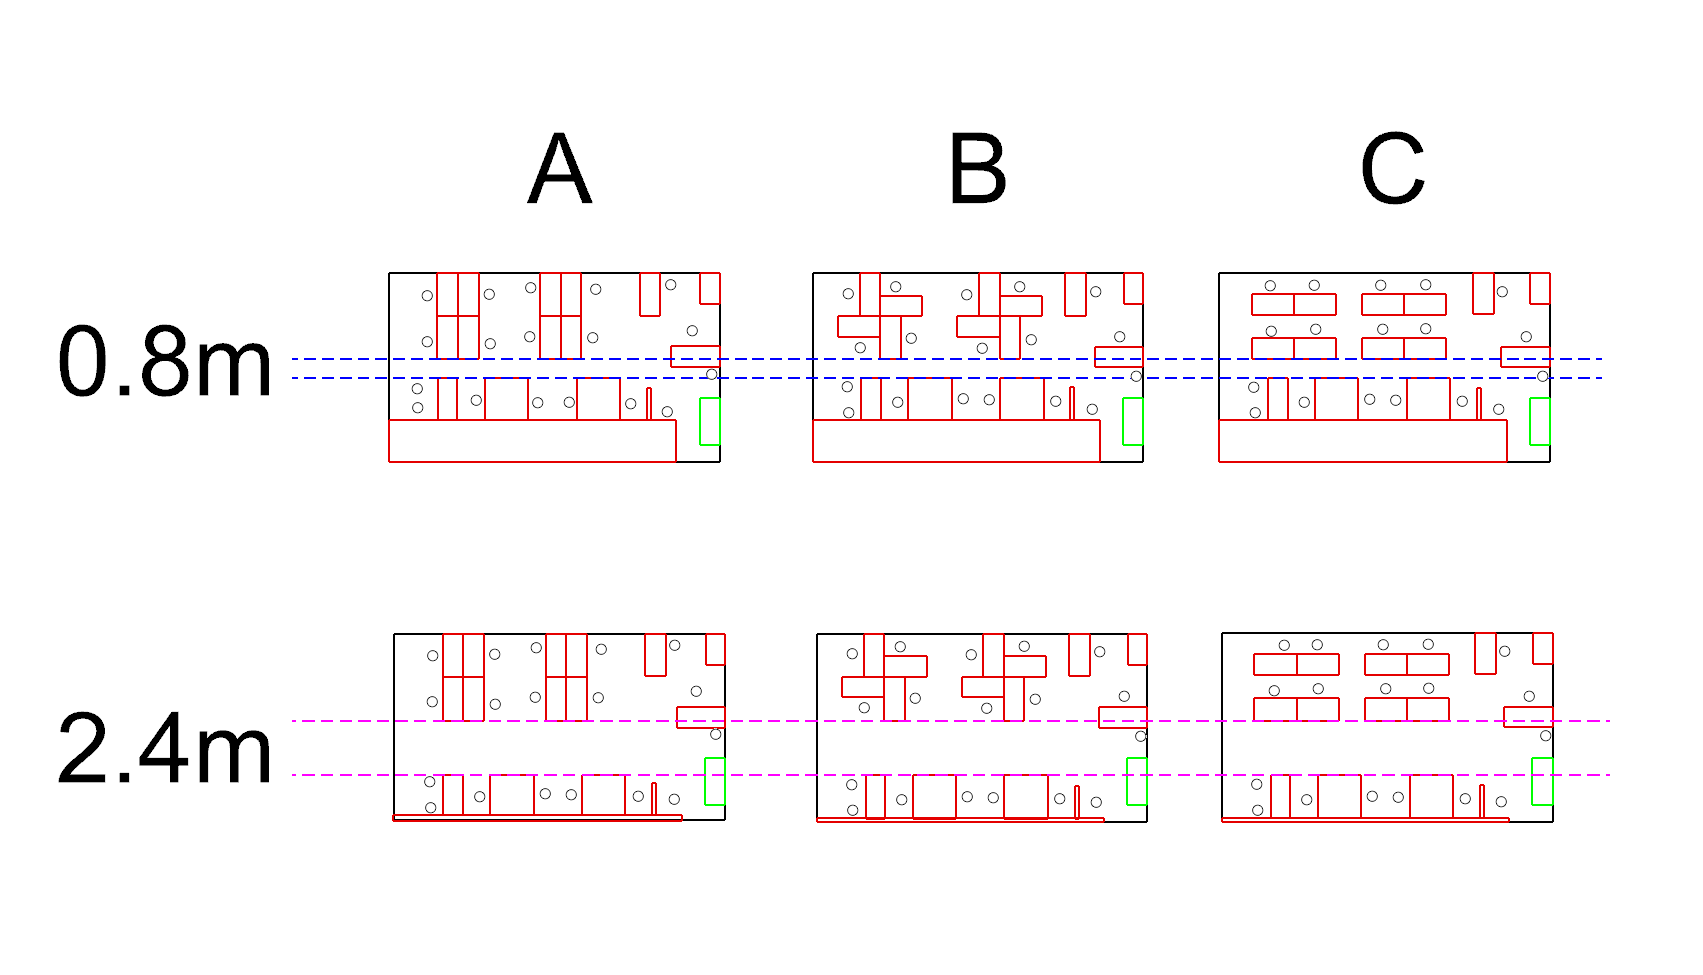
\includegraphics[width=\textwidth]{WidthCompare.png}
    \caption{Corridor Width}
    \label{fig:corridorwidth}
\end{figure}

Exit Configuration \ref{fig:ExitConfiguration}: Single exit and double exit, comparing the impact of different exit quantities on path formation and congestion.
\begin{figure}[h]
    \centering
    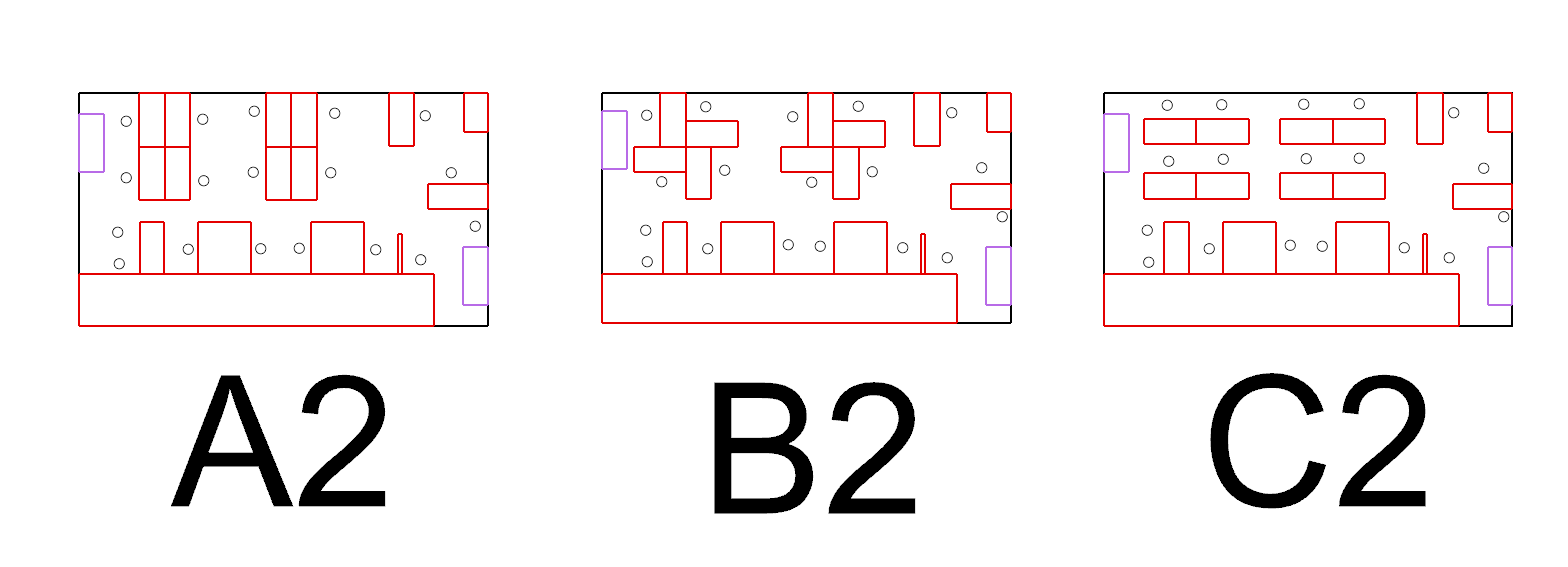
\includegraphics[width=\textwidth]{abc2.png}
    \caption{Exit Configuration}
    \label{fig:ExitConfiguration}
\end{figure}

\subsection{Big Prototype Variables}
We firstly conducted a primitive simulation on the original big prototype. And then we designed two main variable groups based on the primitive simulation results:
\\
Gate width before the exit(the bottleneck) \ref{fig:4ExitsGate}:
\(g\in[1.0,1.6]\text{m}\) is to assess sensitivity of early queuing, discharge rate, and lane merging.
\begin{figure}[h]
    \centering
    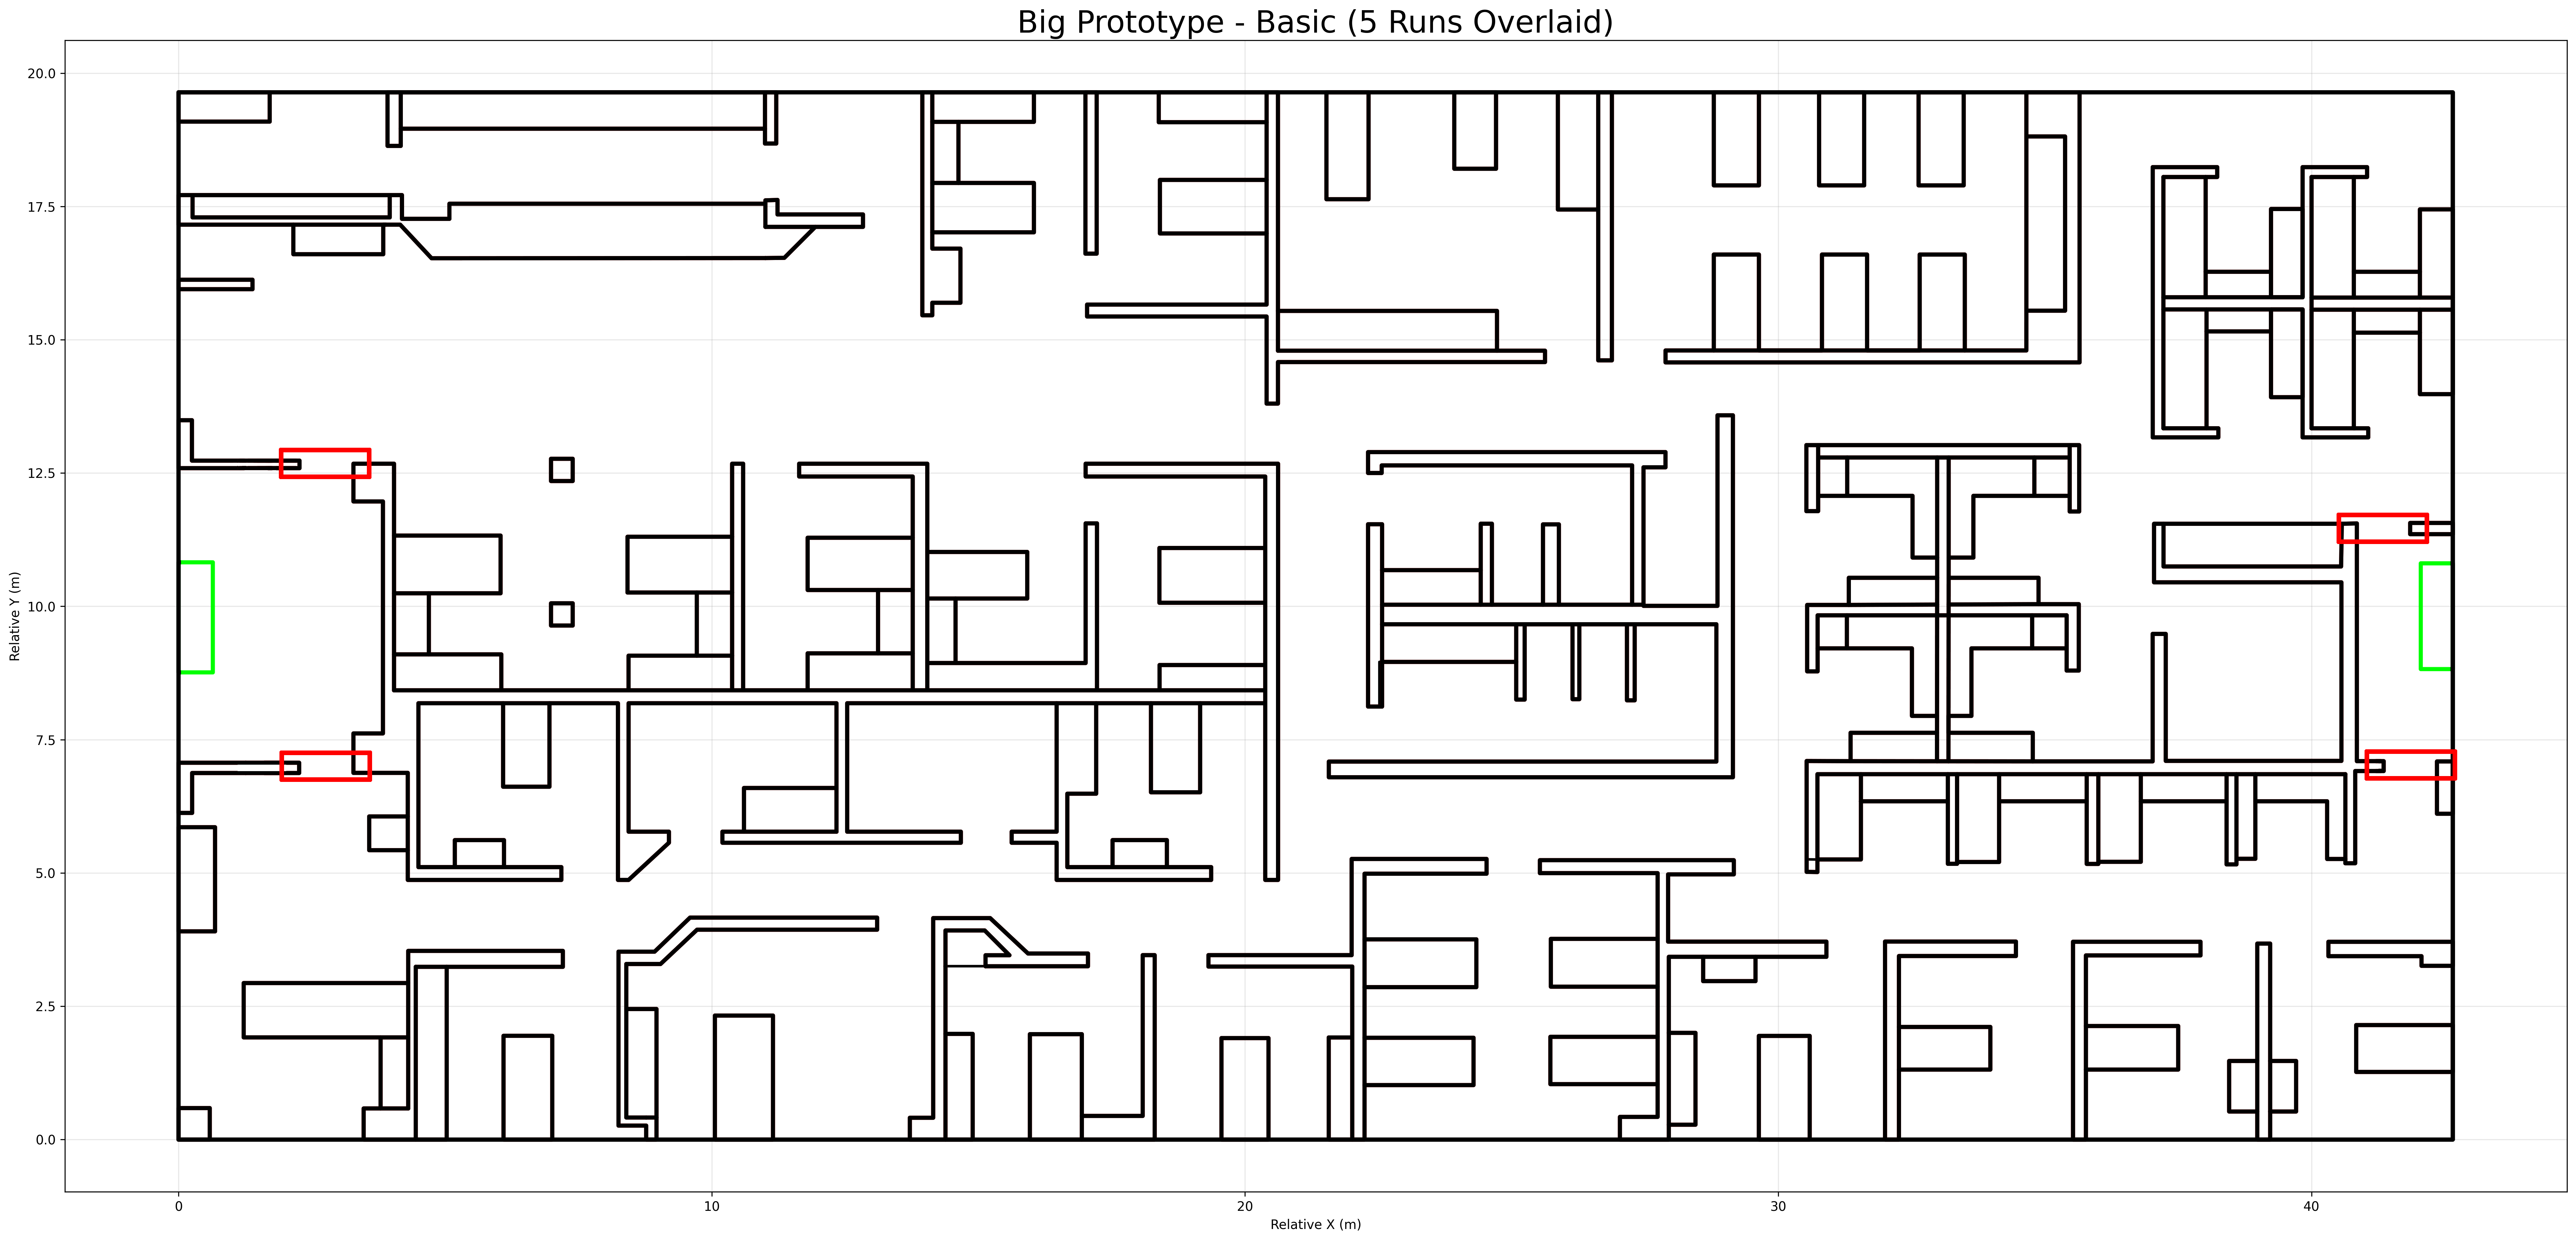
\includegraphics[width=\textwidth]
    {trajectory_overlay_layout_4ExitsGate.png}
    \caption{Change of the gates width before the exits}
    \label{fig:4ExitsGate}
\end{figure}
\\Room-Corridor Coupling: According to the primitive simulation \ref{fig:bigprimitive}, with red lines in the figure representing agent trajectories from all the five runs, the trajectories show convergence into three main corridor segments: corridor a (upper), corridor b (lower-left), and corridor c (lower-right). To quantify the combined effects of "room entrance(blue) and corridor gate(red) width" on the flow distribution and congestion of these main passages, we conducted a full factorial cross-experiment using room door width and corridor gate width entering a/b/c as core independent variables: room door width and gate width in range of {1.0, 1.2, 1.4, 1.6}m. For each combination, we evaluated its impact on early queuing, throughput capacity, and the merging and conflict patterns of the three corridors. 
\begin{figure}[h]
    \centering
    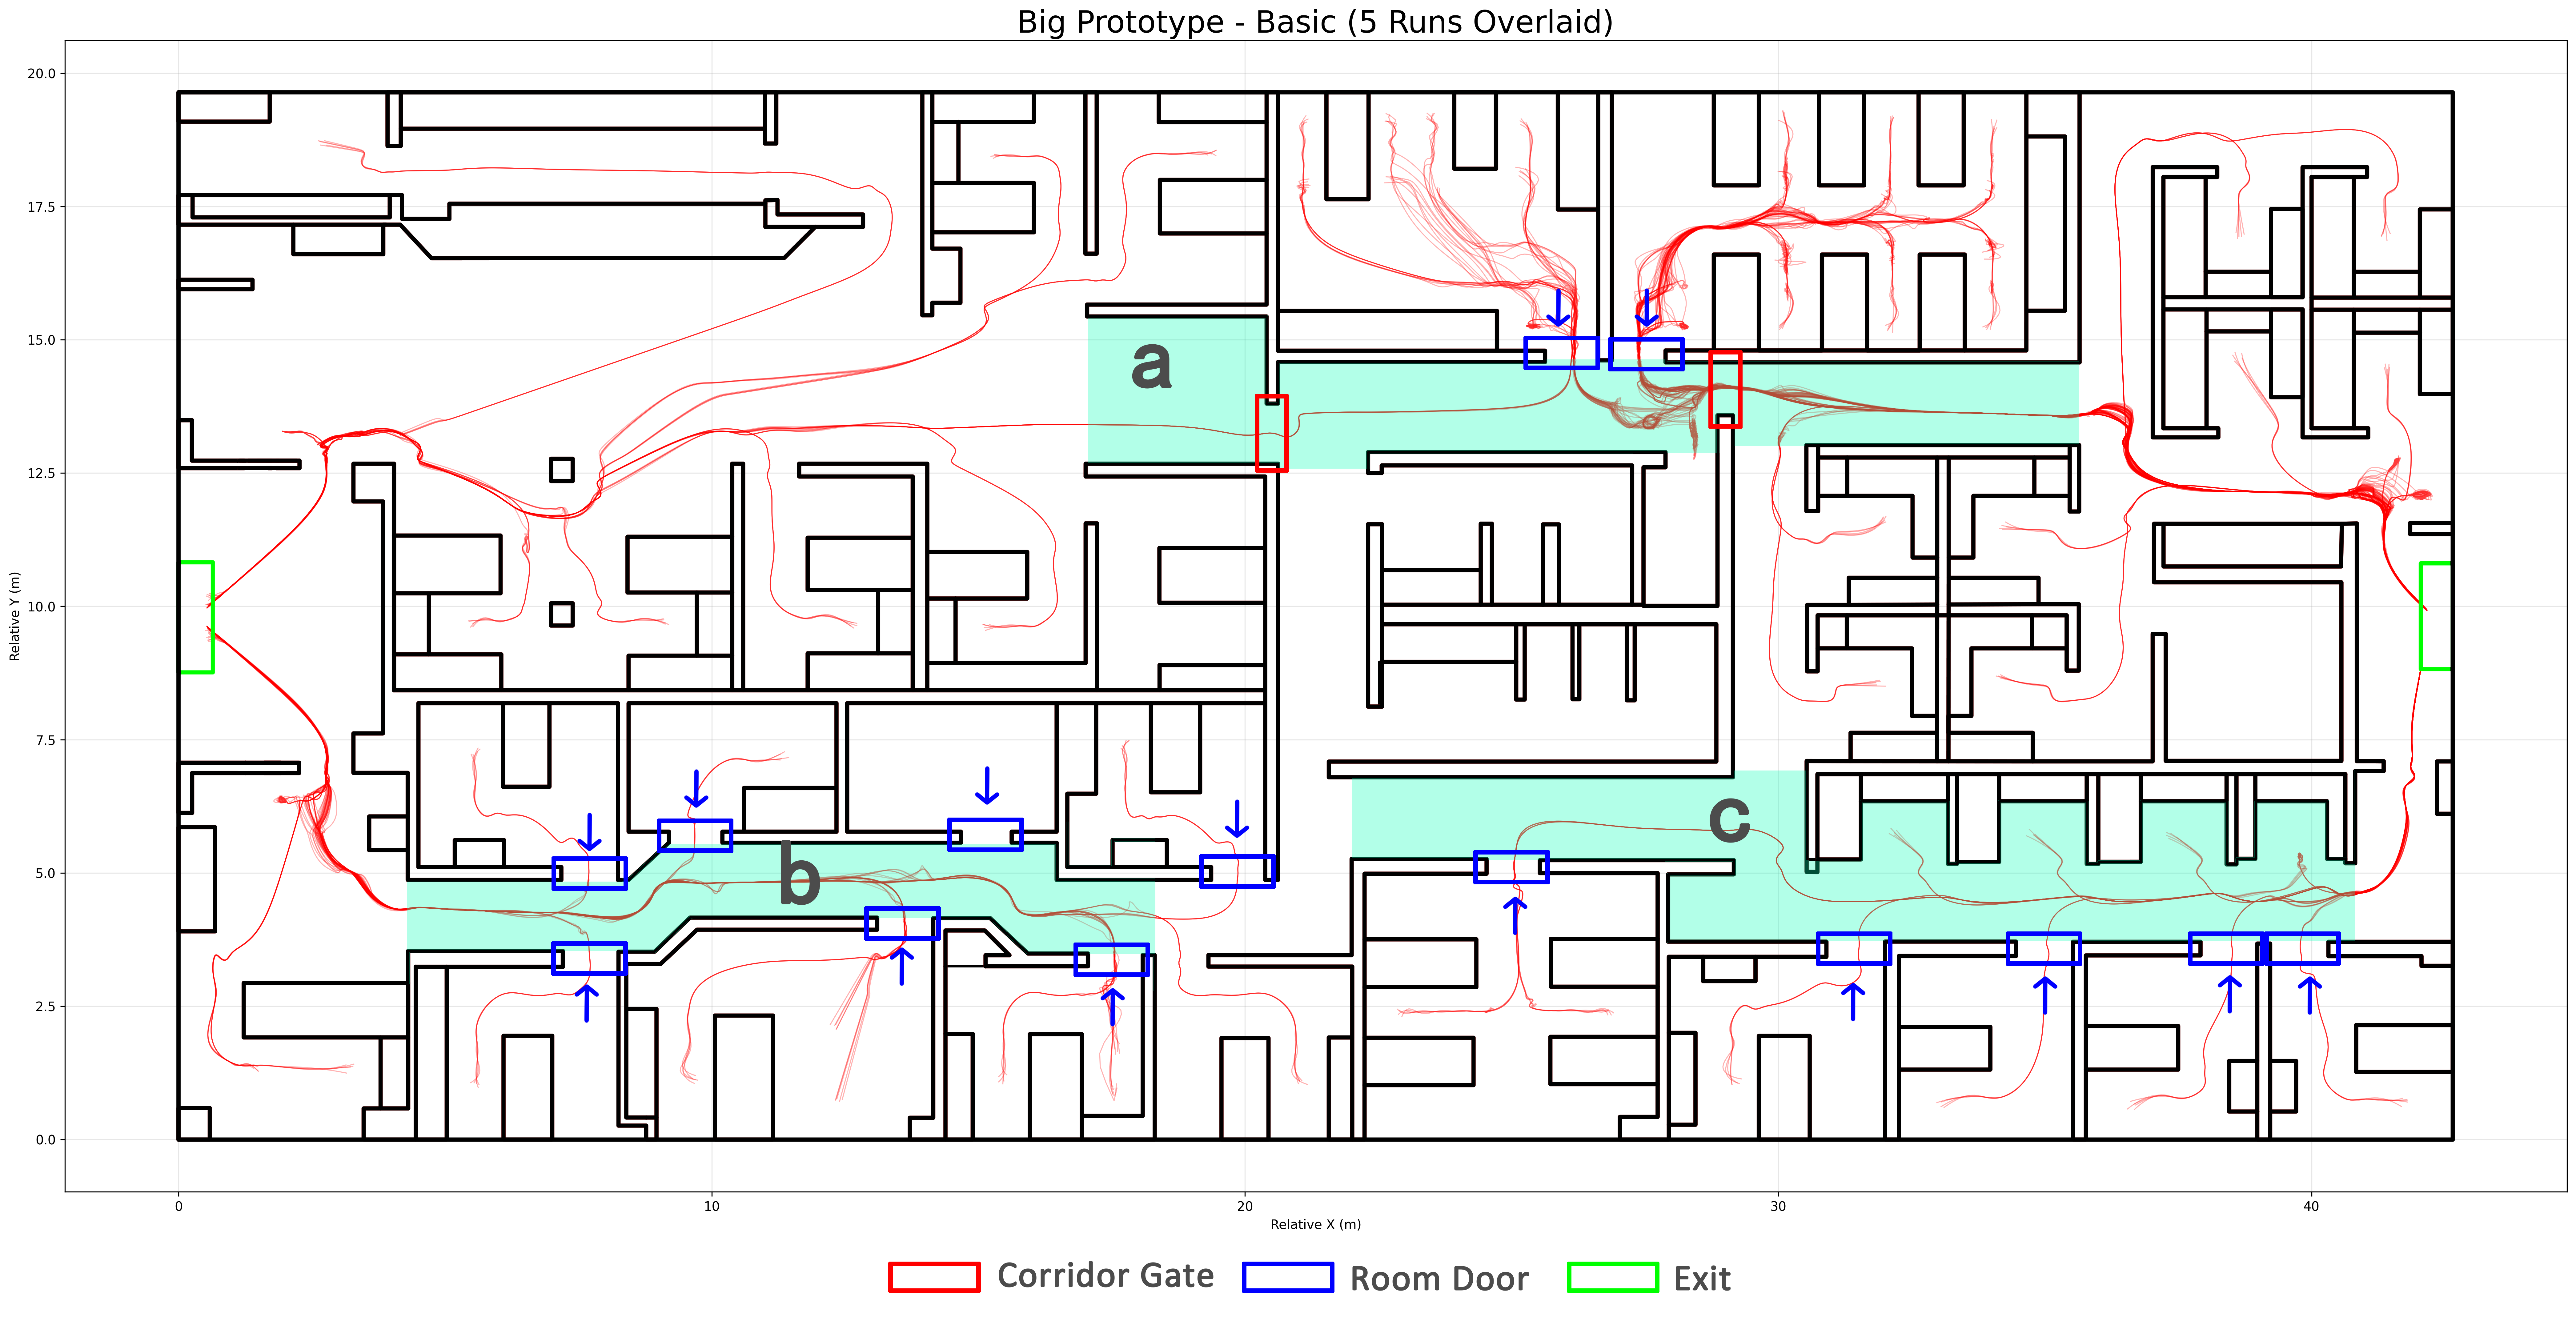
\includegraphics[width=\textwidth]{trajectory_overlay_layout_CorridorAnalysis_Basic.png}
    \caption{Trajectories on the original big prototype and main corridor segments}
    \label{fig:bigprimitive}
\end{figure}

\section{Agents and Model Settings}

This section focuses on clearly setting and recording the attributes of agents (pedestrians), the initial distribution, and the key parameters of the Social Force Model (SFM) within the JuPedSim framework, ensuring comparability and repeatability between different configurations.

\subsection{Agent Attributes and Initial Conditions}

Initial Agent Quantity and Distribution: The total number of agents is set in the Grasshopper/JuPedSim scene input based on the scale of the scenario, with the initial distribution (Grasshopper point set) controlling the initial quantity and spatial distribution.
\\Initial Position Mapping: The point set of Grasshopper is mapped to the initial coordinates of the agents, ensuring that the randomness of initial positions between different configurations is controllable and that repeated experiments can be replicated.
\\Goals and Behavioral Tendencies: Defaults are uniformly set, but in scenarios with multiple entrances, agents tend to choose the shortest path.

\subsection{Social Force Model Parameters}

Model Framework: The built-in Social Force Model of JuPedSim is used as the core microscopic simulation model.
\\Desired Speed: 0.8 m/s is set as the default value, with sensitivity analysis within a range (e.g., 0.6-1.0 m/s) conducted as needed.
\\Interaction Force Parameters: These include repulsive forces between agents, repulsive forces against obstacles, and response intensity to queuing and group aggregation. The initial settings adopt the official recommended values from JuPedSim.
\\Obstacle Handling and Boundary Conditions: The obstacle force scale is set to 1000 to balance the resistance to obstacles in complex scenarios, preventing excessive suppression of agent movement. Boundary conditions follow the wall and exit definitions in the geometric input of the scene.

\section{Data collection and Analysis}

\subsection{Data Output and Storage}
Each simulation produces an independent SQLite database file, recording agent trajectories, speeds, positions, and scene metadata for easy playback and offline analysis.
\subsection{Data Reading and Processing}
Use JupyterLab and Python to read SQLite files (sqlite3), organizing the data into an analyzable structure (DataFrame), and aggregating and statistics on time steps, agent attributes, congestion indicators, etc.

\subsection{Indicators}
\subsubsection{Primary Indicators}
Total Evacuation Time (TET): The overall comparison of evacuation performance under various configurations, which can be presented by evacuation time tables and line charts.
\\
Path Distribution Characteristics: Visualized through trajectory patterns in speed-trajectory diagrams.
\\
Congestion Hotspot Distribution (Hot Zones/Density): The location and extent of low-speed clustering and congestion areas in speed-trajectory diagrams, which equivalently display congestion hotspots and their migration patterns.
\\
\subsubsection{Secondary Indicators}
Path Formation Patterns: Identification of single-lane and double-lanes flow, lane convergence, bottleneck queuing patterns, and their locations based on the trajectory morphology analysis.
\\
Repeated Interval Fluctuation (Robustness): Line overlap/error band performance across multiple runs under identical parameters, expressed as minimum-maximum ranges or mean ± deviation to indicate fluctuation levels.

\subsection{Results Presentation and Visualization}
This study uses Total Evacuation Time (TET) as the primary evaluation metric. For each parameter level (such as door width, corridor width, and exit configuration), we calculate the mean TET and fluctuation range from multiple independent simulations, and conduct direct comparisons and ranking based on these results. To identify potential threshold effects, we observe slope changes in evacuation time line graphs, record parameter intervals where significant inflection points or plateau segments occur, and select representative parameter points to compare with velocity-trajectory diagrams to explain the mechanistic differences in "convergence-merging-queuing" patterns as parameters vary. To ensure the stability of conclusions, each parameter combination incorporates randomized agent initial positions with five repeated experiments.
%%%%%%

\chapter{Result and Discussion}
\label{resultChapter}
\section{Small Prototype}
\subsection{Overview}
\begin{figure}[h]
    \centering
    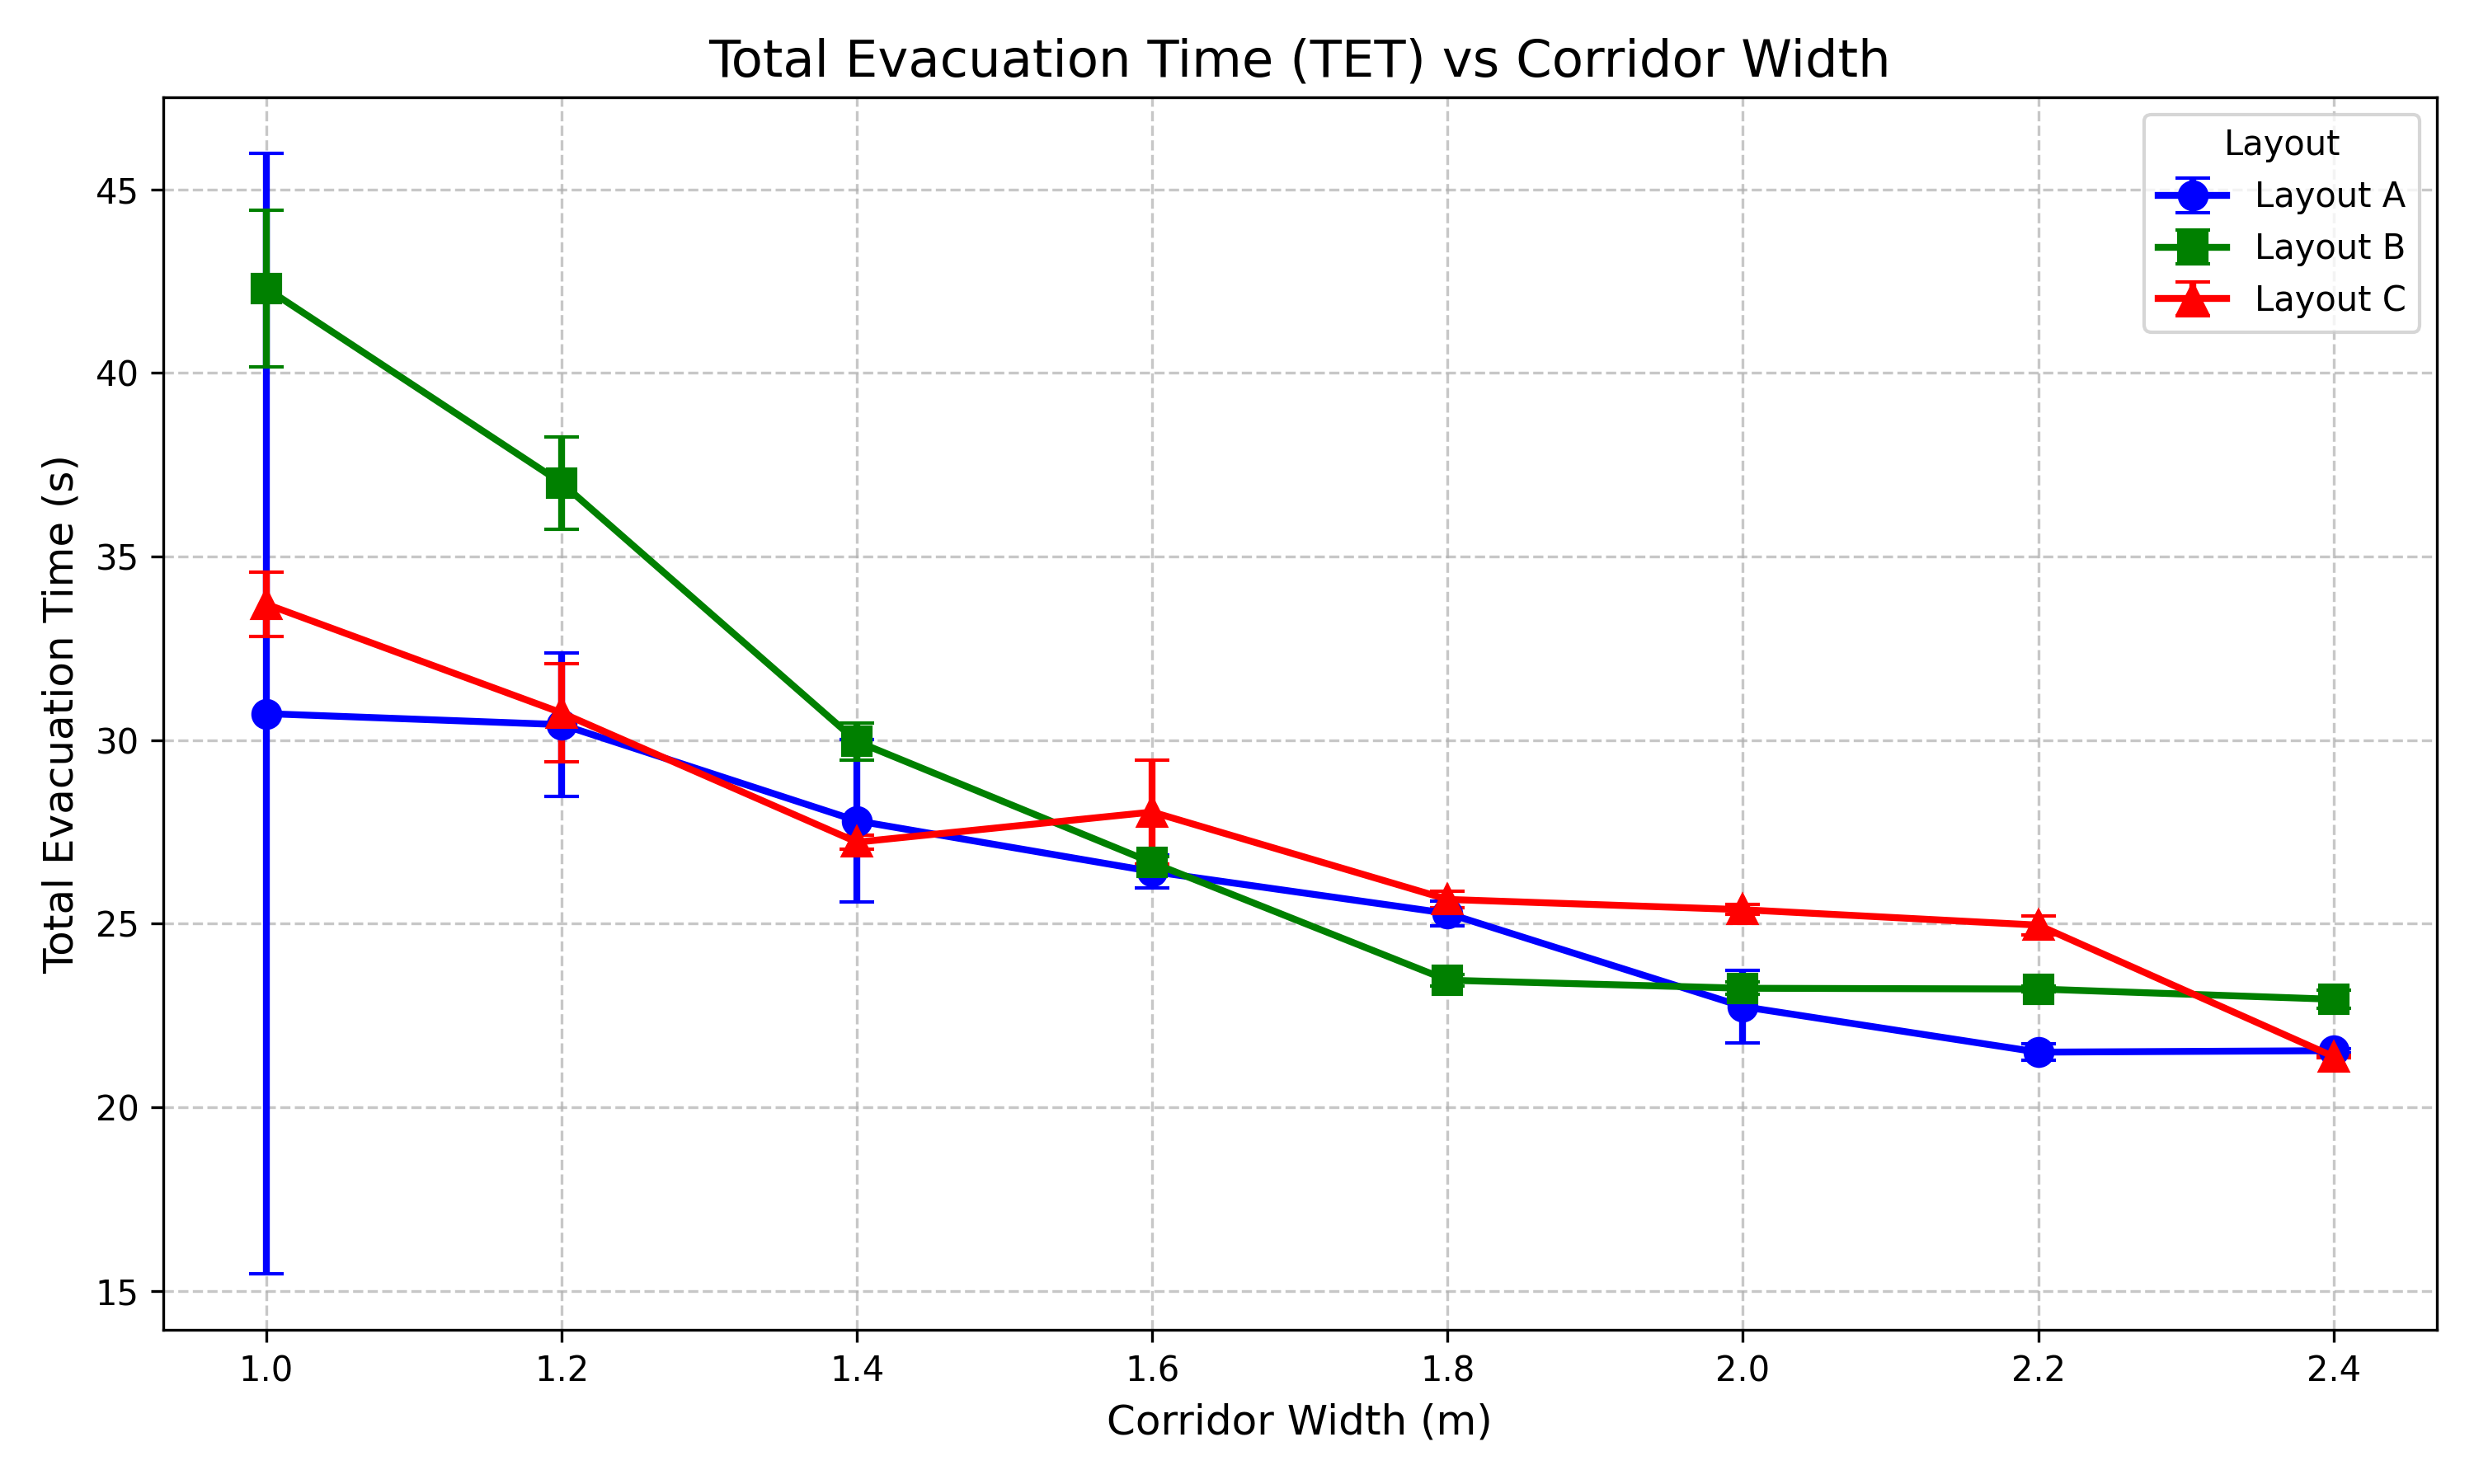
\includegraphics[width=\textwidth]{tet_vs_width.png}
    \caption{TET vs Corridor Width}
    \label{fig:tet_vs_width}
\end{figure}
The results of this study \ref{fig:tet_vs_width} indicate that the wider the corridor, the shorter the TET, but the returns from widening do not increase linearly. Within the range of approximately 1.0-1.6/1.8 m, even a slight increase in width can lead to a significant reduction in time; when the width approaches or exceeds 2.0 m, continued widening still provides benefits, but the magnitude is no longer substantial. This aligns with everyday experience: in very crowded spaces, even a small additional passageway can help disperse the flow of people; however, when the space is not particularly crowded to begin with, adding more passageway does not yield such noticeable improvement.

\subsection{Speed and Trajectories Analysis}
Looking at the speed and trajectories of Layout A \ref{fig:speed_trajectory_layout_A},B \ref{fig:speed_trajectory_layout_B},C \ref{fig:speed_trajectory_layout_C}, as the width increased from 1.0m to 1.6-1.8m, the main corridors of the three layouts generally transformed from a crowded zone to two relatively stable parallel lanes. The speed chart shows that the originally continuous red and yellow bands have been replaced by two greener bands, and the slow zone has significantly contracted. This indicates that the increase in width first reduces lateral friction and frequent evasive maneuvering, allowing individuals to maintain a speed close to free-flow for a longer period of time. In terms of the TET, this stage has the largest reduction, and the result fluctuations of each layout have simultaneously decreased.

\begin{figure}[h]
    \centering
    \includegraphics[width=\textwidth]{speed_trajectory_layout_A.png}
    \caption{Speed and Trajectories for Layout A}
    \label{fig:speed_trajectory_layout_A}
\end{figure}

The main corridor in Layout A is relatively straight, with multiple tributary inflow points along the line. The trajectory and velocity diagrams show that tributaries have already formed orderly queues before reaching the confluence point, with only mild short-distance deceleration when entering the main corridor. This suggests that conflicts are resolved in advance within the tributaries, with stable dual lanes forming starting from corridor widths of 1.6 m, while widths of 2.0-2.4 m maintain only small deceleration zones before the final exit. As a result, medium to high-width sections have lower average times, smaller variances, and higher speed limits. Furthermore, as width increases, evacuation time decreases relatively steadily.

\begin{figure}[h]
    \centering
    \includegraphics[width=\textwidth]{speed_trajectory_layout_B.png}
    \caption{Speed and Trajectories for Layout B}
    \label{fig:speed_trajectory_layout_B}
\end{figure}

Layout B contains multiple T-shaped or cross intersections with dispersed confluence points. Under corridor widths of 1.0-1.4 m, the lower section near intersection points repeatedly experiences team breaking and regrouping phenomena. The visual manifestation in the diagram is the formation of multiple mesh-like low-speed zones, with numerous congestion points covering a wide range. After widening the width to 1.6 and 1.8 m, these mesh-like low-speed zones significantly diminish and form lanes, which indicates that widening the corridor width can effectively avoid interactive conflicts, resulting in the greatest time reduction. However, at 2.4 m, some remaining light yellow zones are still visible, causing the speed limitation at the high-width stage to be slightly lower than layouts A and C.

\begin{figure}[h]
    \centering
    \includegraphics[width=\textwidth]{speed_trajectory_layout_C.png}
    \caption{Speed and Trajectories for Layout C}
    \label{fig:speed_trajectory_layout_C}
\end{figure}

Layout C \ref{fig:speed_trajectory_layout_C} employs parallel lanes upstream, which allows agents to form queues before merging into the main corridor, showing better organization than Layout B. However, merging still requires navigating through a turning angle, resulting in a relatively low overall speed limitation. As shown in \ref{fig:tet_vs_width}, Layout C exhibits an abnormal fluctuation at 1.6 m width, where evacuation time is actually longer than that of the 1.4 m corridor width. Comparing the speed and trajectory diagrams for 1.4 m and 1.6 m cases, we can observe that in the 1.6 m scenario, although attempts are made to form two lanes in the bottleneck area before the exit and the merging zone below, the centerline distance between the two lanes remains too close. This intuisively results in a great increase in lane width, reflecting more friction and avoidance behavior, which matches the Social Force Model's description. After the width increases to 1.8-2.0 m, the inter-lane spacing and merging diffusion angle increase, the slow-speed zones are eliminated, and evacuation performance rapidly improves. At the width of 2.4 m , the turning angle effect becomes essentially negligible, and the speed limitation exceeded that of Layout A.

Among the three layout types, stable low-speed zones most commonly appear at the following locations: intersections or merging areas, sharp turns and convergence sections before exits. Increasing width makes these low-speed zones shorter, shallower and less frequent. This may indicate that corridor width is not a direct contributing factor. Rather than continuing to widen corridors blindly when the corridor width is already relatively wide, it would be better to optimize these low-speed zones, such as extending merging transitions, reducing merge angles and increasing directional guidance and one-way organization.

\subsection{Double Exits Comparison}
According to Figure \ref{fig:all_tet_vs_width}, after setting up dual exits, the TET for all three layouts decreased overall, with significantly reduced fluctuation between trials. The 1.0-1.6/1.8 m range remains the interval with the fastest efficiency improvement; when the width beyond 2.0 m, the marginal benefits of continued widening disappear, and the curve tends to flatten. Compared to single exit, double exits first reduce the low-speed zones in the terminal convergence section, offering the system a stable state with sufficient capacity. Under double exits condition, the speed and trajectories of all three layouts are more uniform and the trend is smooth, with significantly more green sections, while red and yellow low-speed zones are compressed into shorter localized areas. Agents seperate earlier after they start to evacute, and the backtracking and snake-like movement in the main corridor are notably reduced.

\begin{figure}[h]
    \centering
    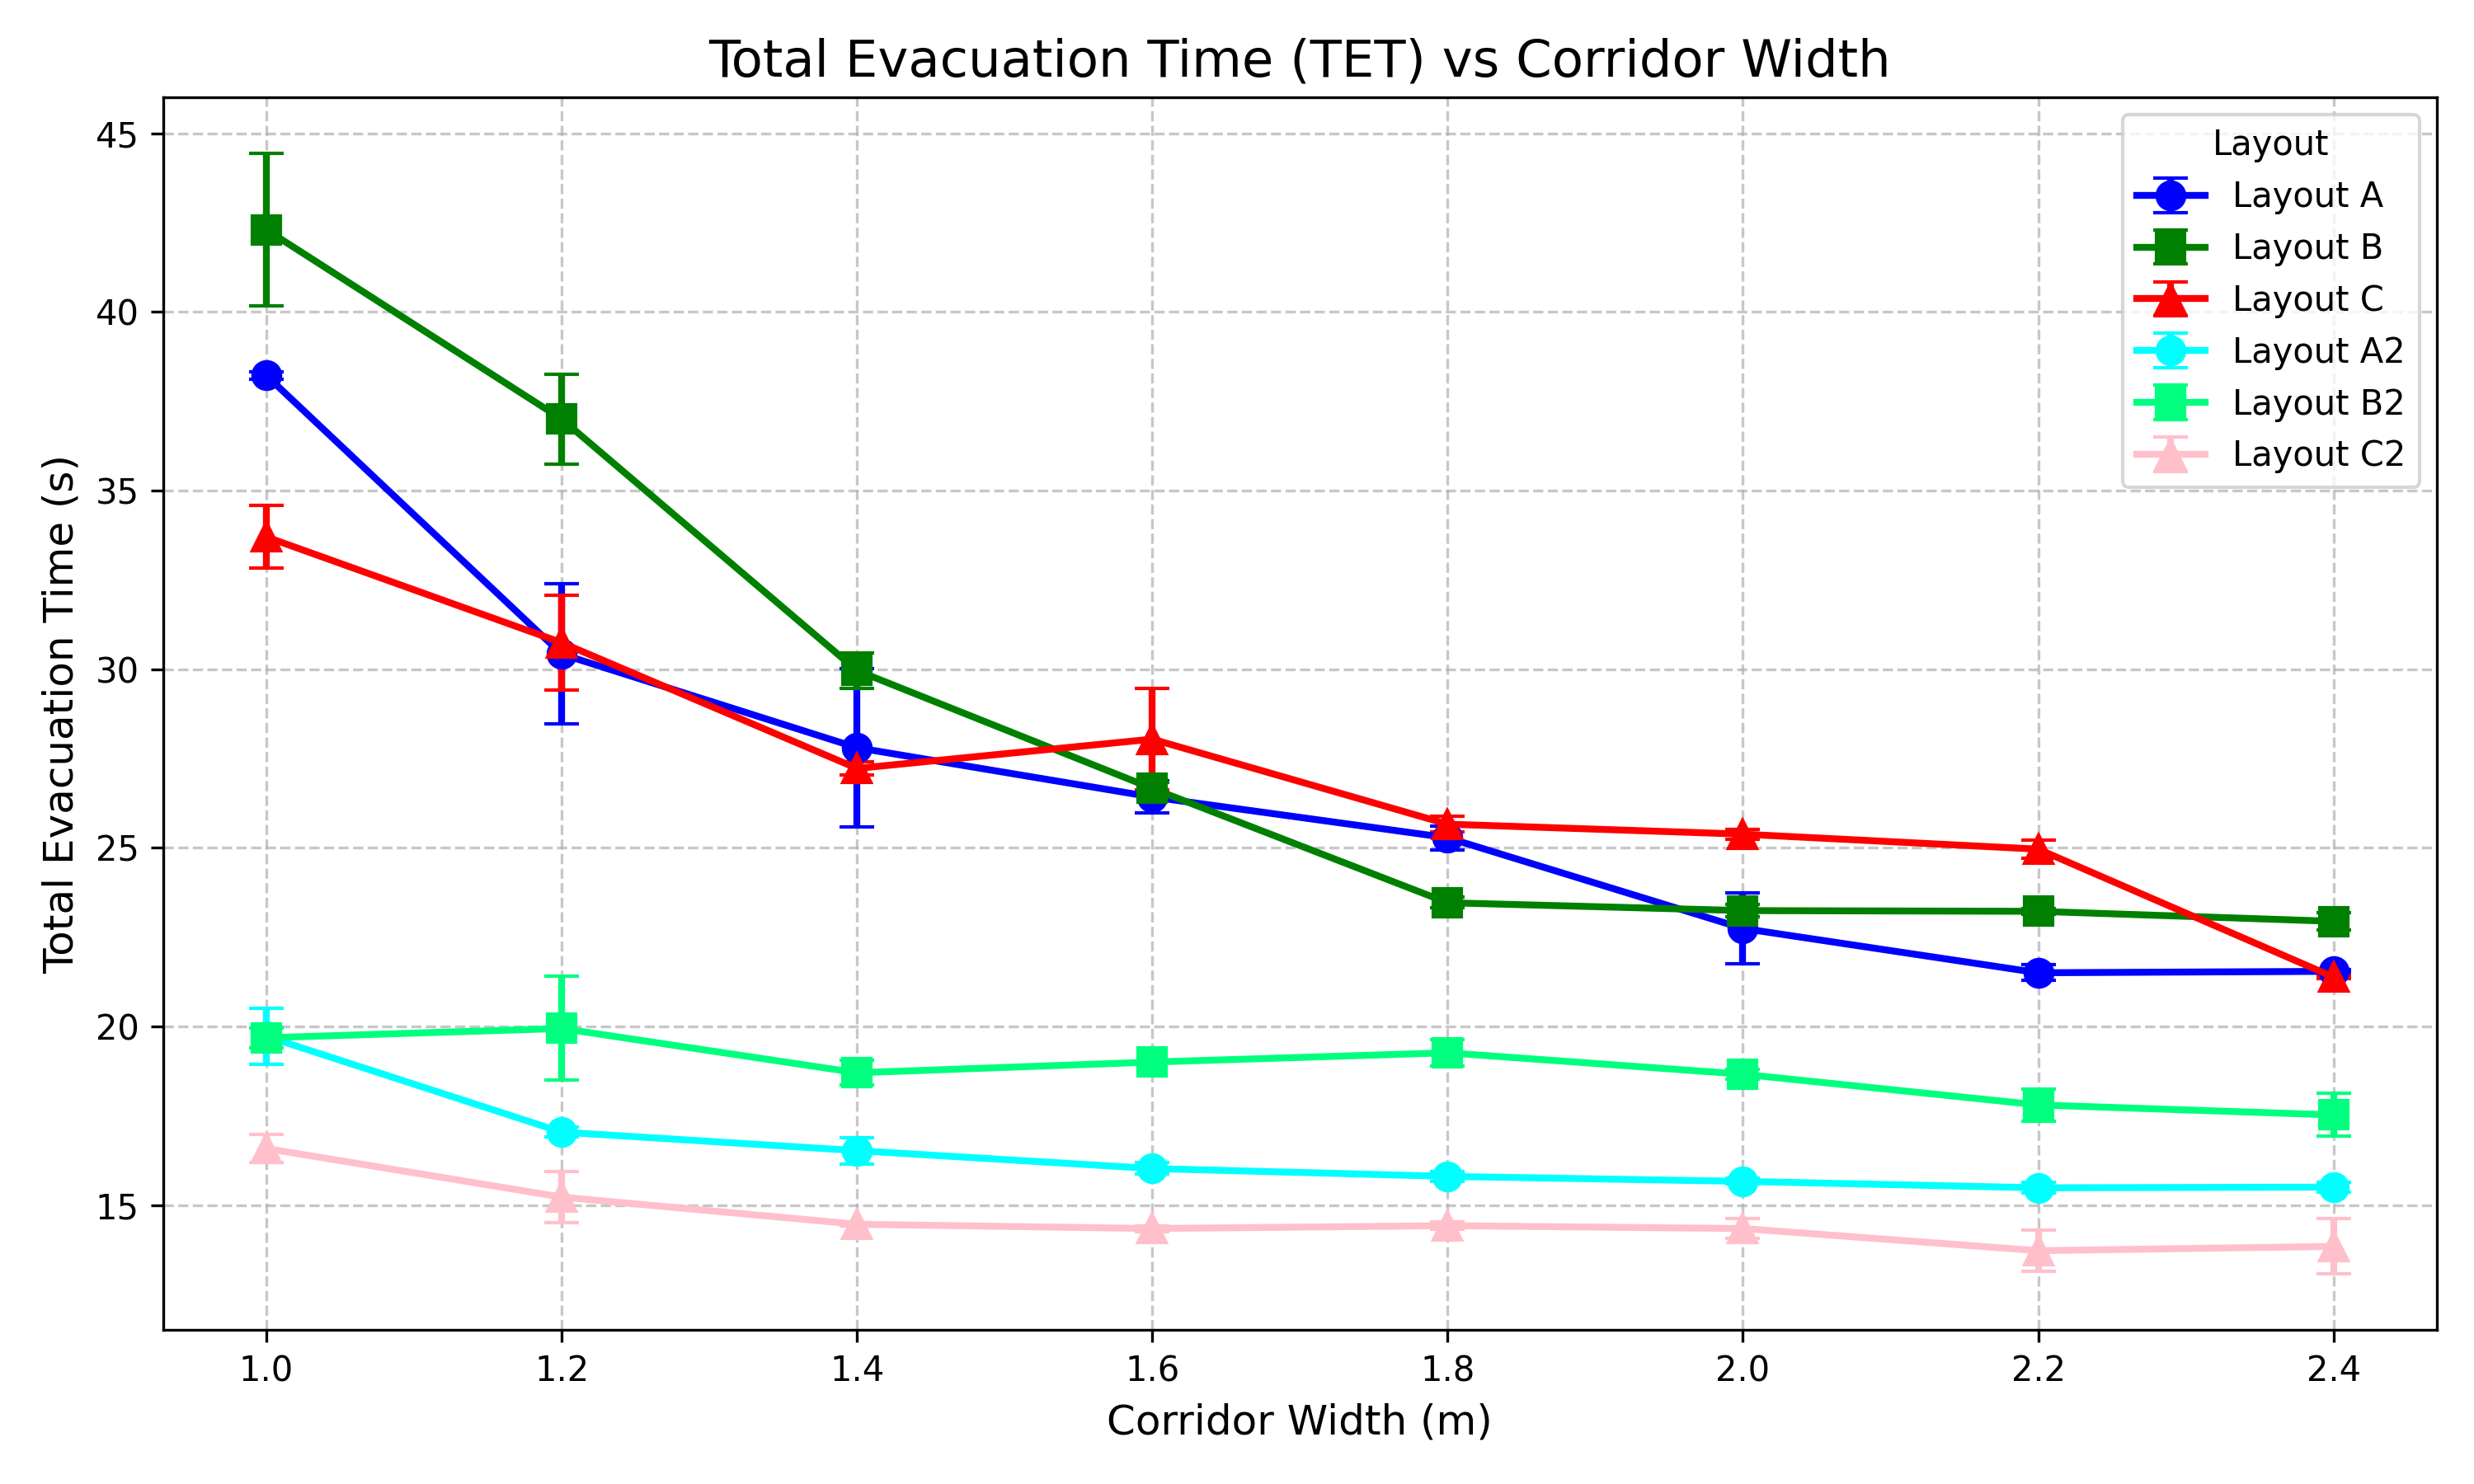
\includegraphics[width=\textwidth]{All_tet_vs_width.png}
    \caption{TET vs Corridor Width for All Layouts with Single and Double Exits}
    \label{fig:all_tet_vs_width}
\end{figure}

\begin{figure}[h]
    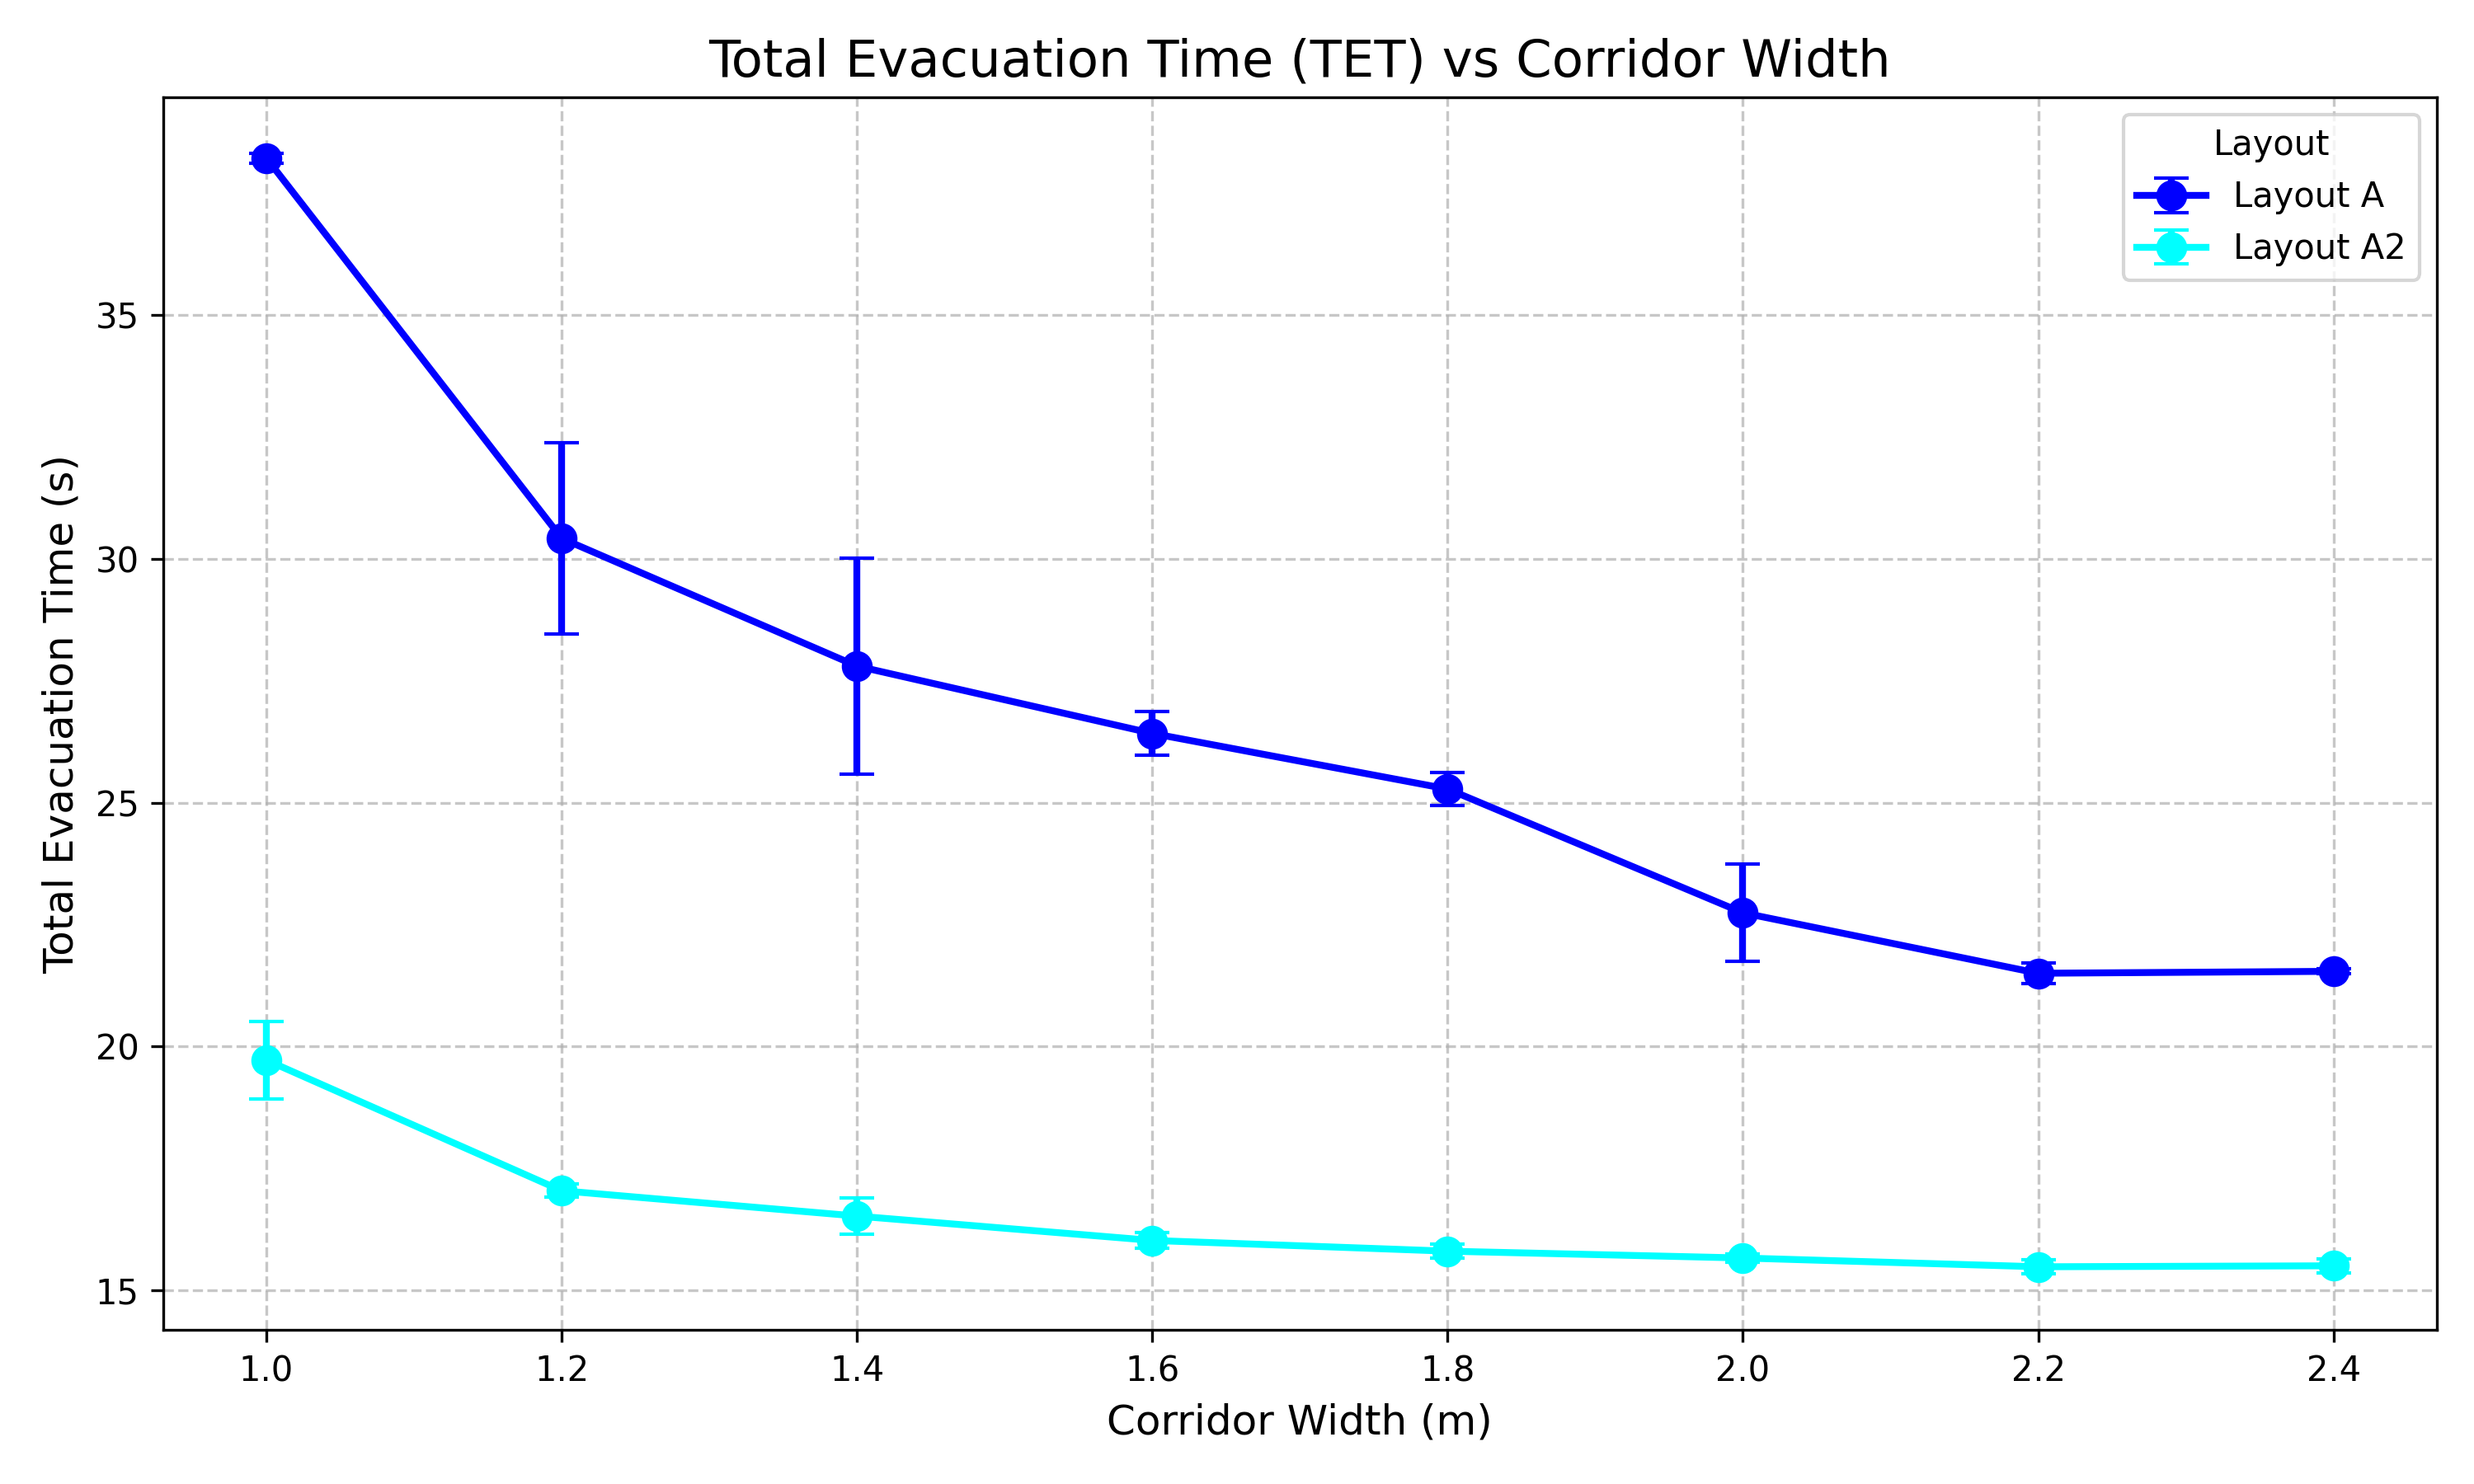
\includegraphics[width=\linewidth]{AvsA2_tet_vs_width.png}
    \caption{TET vs Corridor Width between A and A2}\label{fig:AvsA2_tet_vs_width}
\end{figure}

\begin{figure}[h]
    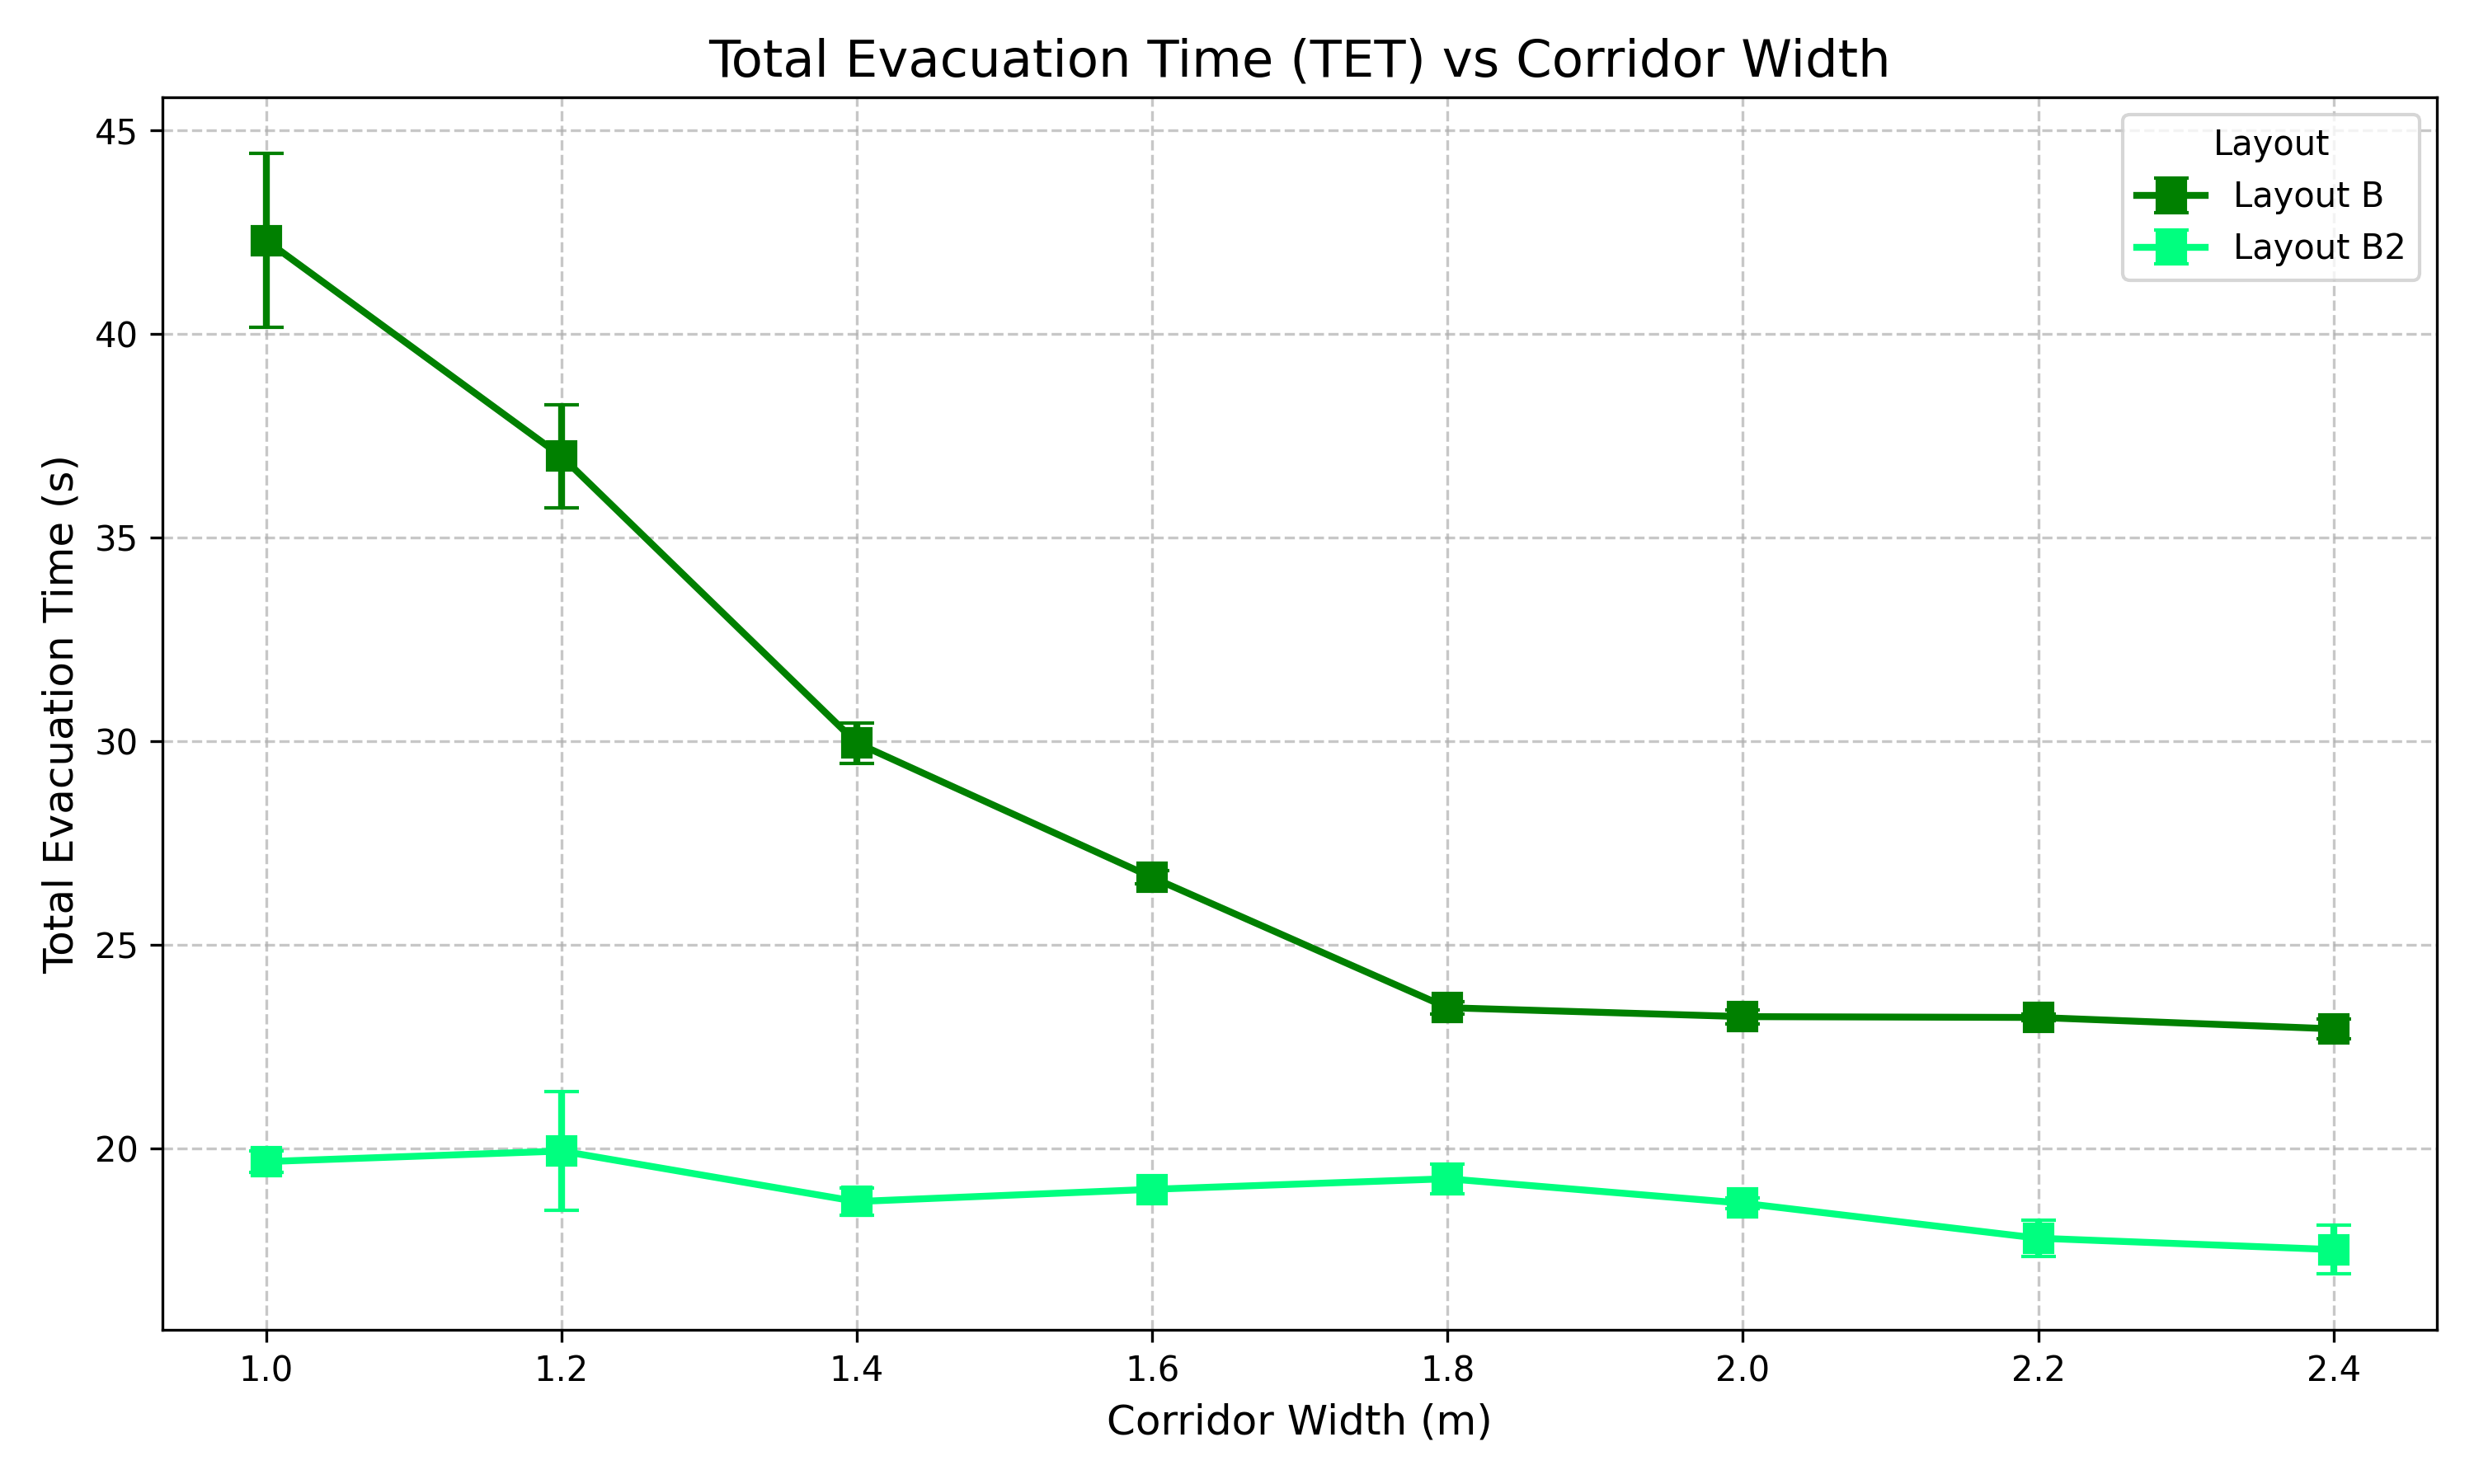
\includegraphics[width=\linewidth]{BvsB2_tet_vs_width.png}
    \caption{TET vs Corridor Width between B and B2}\label{fig:BvsB2_tet_vs_width}
\end{figure}

\begin{figure}[h]
    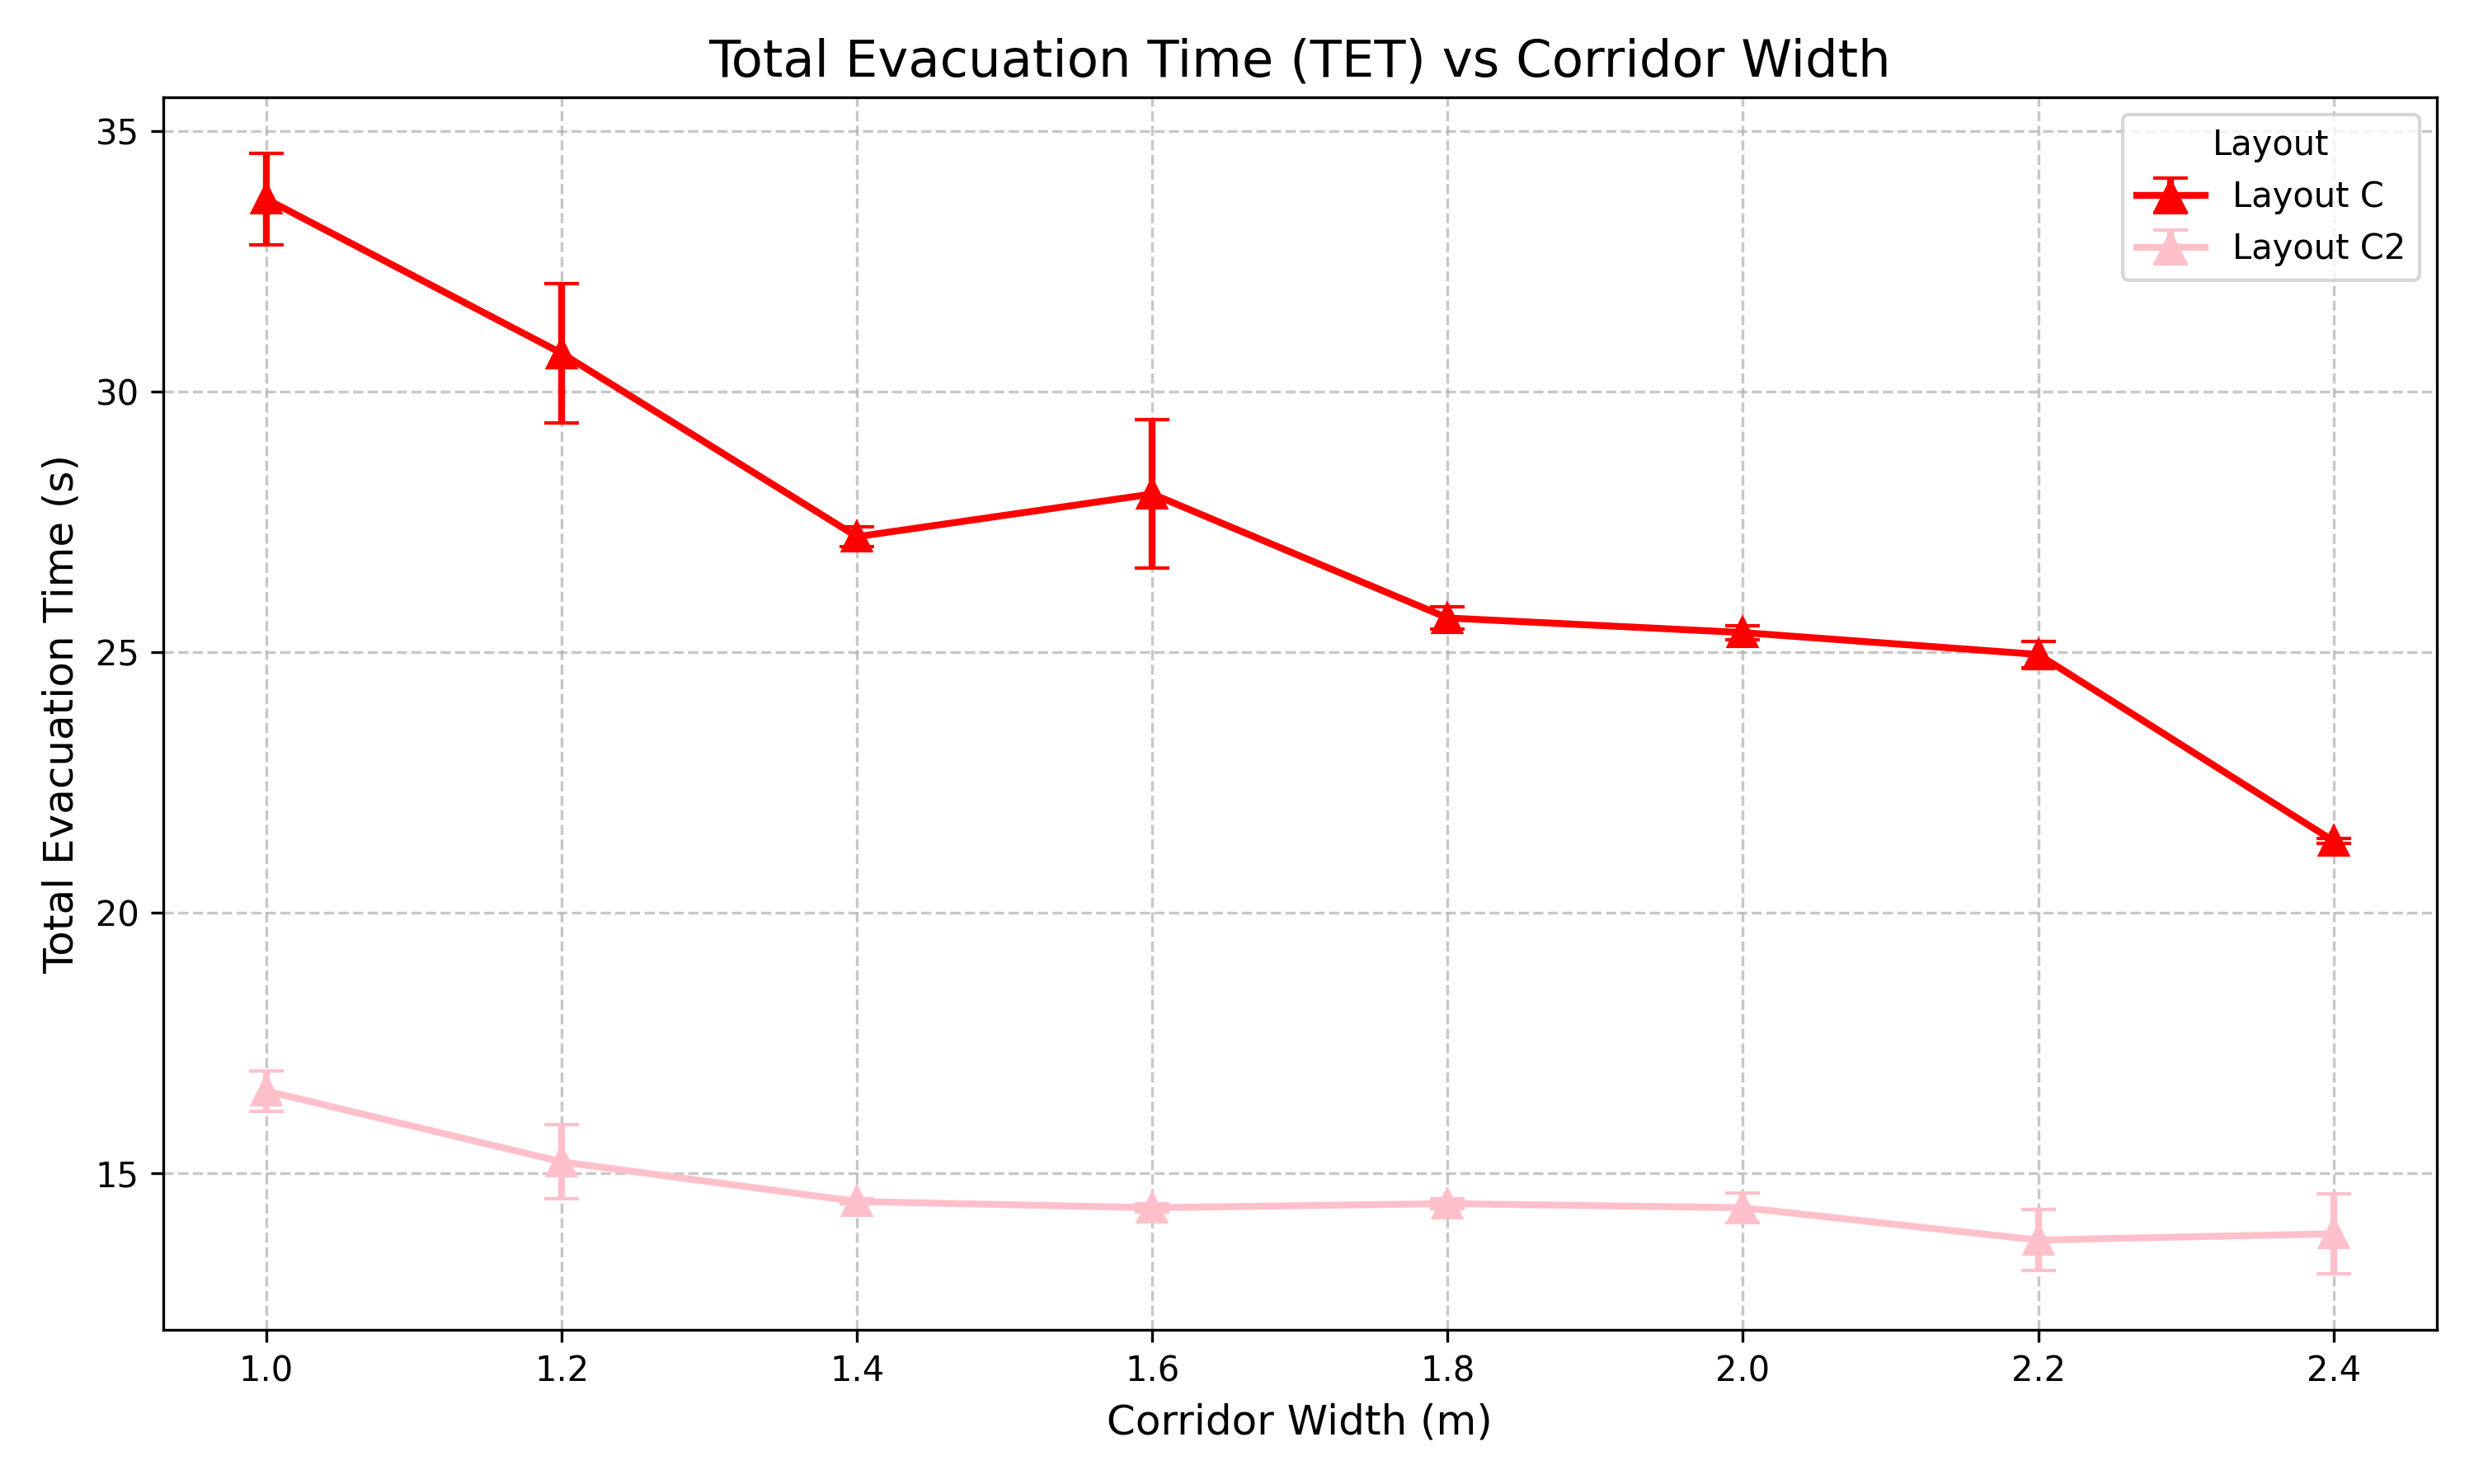
\includegraphics[width=\linewidth]{CvsC2_tet_vs_width.png}
    \caption{TET vs Corridor Width between C and C2}\label{fig:CvsC2_tet_vs_width}
\end{figure}
Under single exit condition, Layout A \ref{fig:speed_trajectory_layout_A} can easily form a continuous low-speed zone before the exit. Although relatively stable double lanes have appeared in the middle section, the convergence of lanes at the end still causes significant speed reduction and creates certain fluctuations. When it comes to double exits \ref{fig:speed_trajectory_layout_A2}, the flow distribution shifts the merging points towards both side exits, weakening the low-speed zone and leaving deceleration before merging. The trajectories show almost no congestion or fluctuation, with the main green flow band extending throughout the entire length. The result shows that the Layout A2 maintains low and stable TET across all widths, showing that the double-exit design directly eliminates the terminal bottleneck.

\begin{figure}[h]
    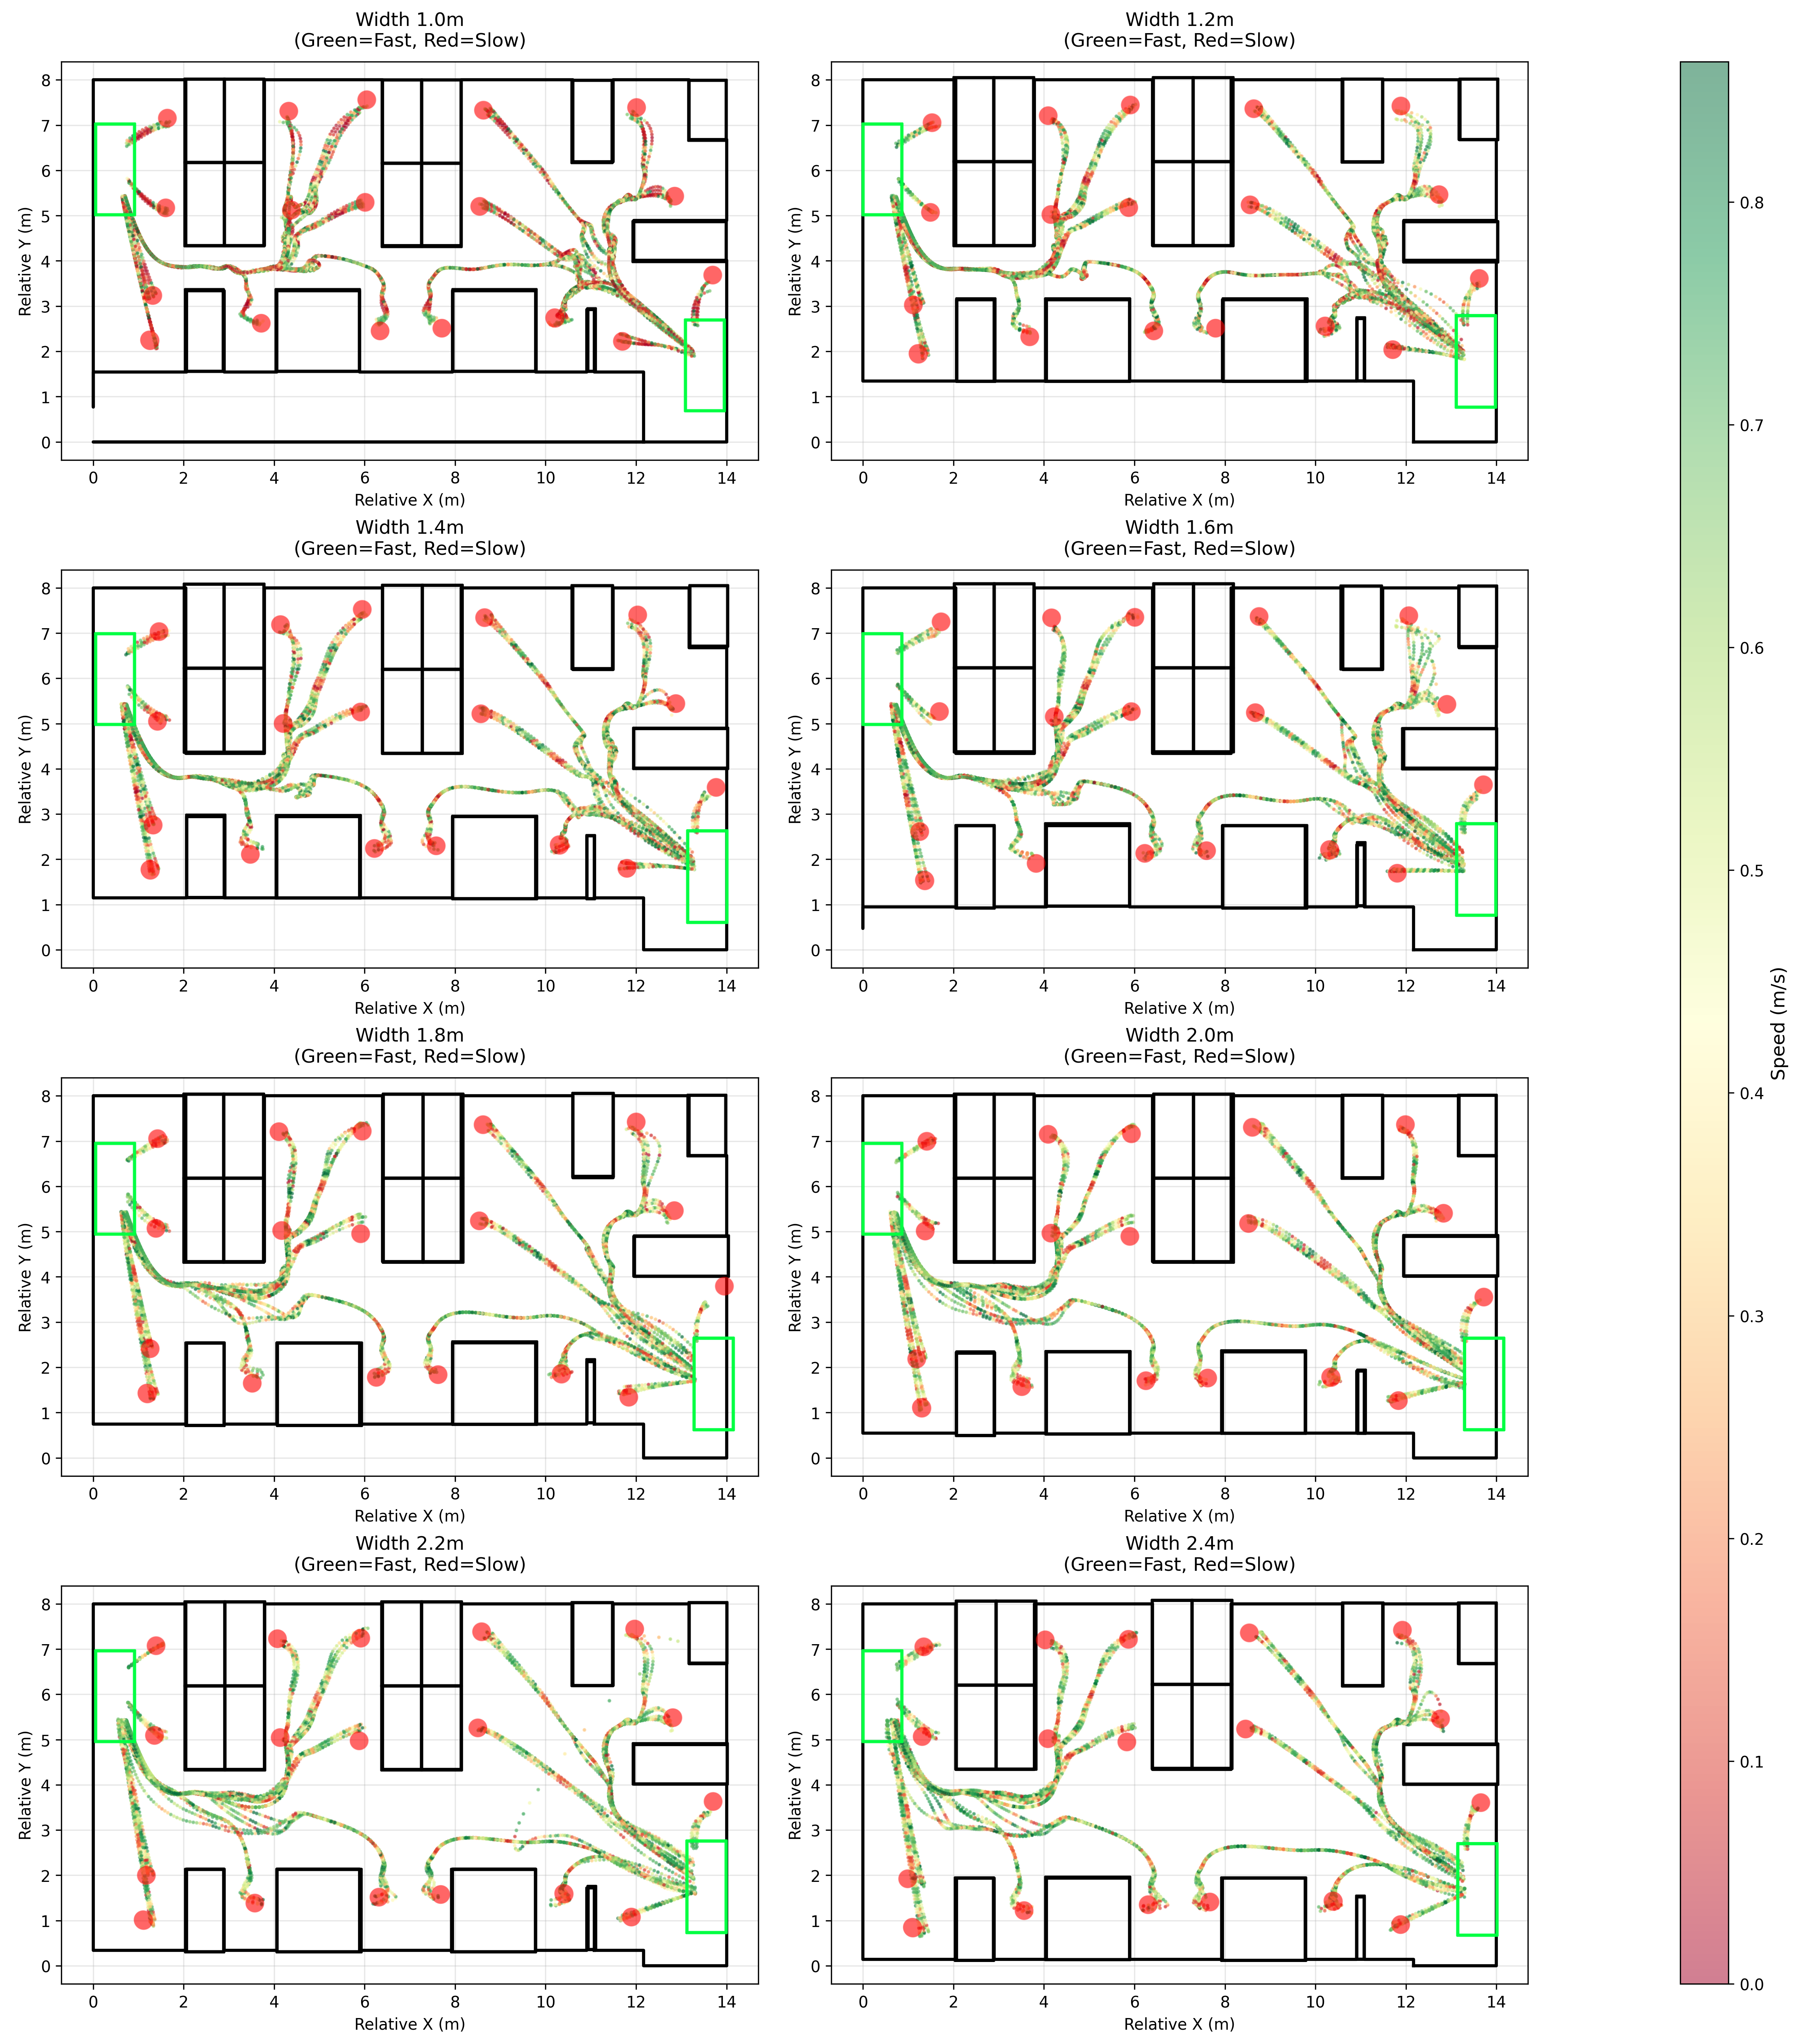
\includegraphics[width=\linewidth]{speed_trajectory_layout_A2.png}
    \caption{Speed and Trajectories for Layout A2}\label{fig:speed_trajectory_layout_A2}
\end{figure}

In single-exit Layout B \ref{fig:speed_trajectory_layout_B}, repeated phenomena of crowd breakup and regrouping occur near multiple intersections, forming a network of red and yellow slow-speed zones on the speed diagram, particularly prominent in the 1.0-1.4 m range. After introducing the second exit \ref{fig:speed_trajectory_layout_B2}, the terminal convergence pressure in Layout B2 was not significantly reduced, with only slight decreases in evacuation time, and even increases in time observed in the condition of 1.2m and 1.4-1.8m corridor width. The reason may be that multiple intersection points are still retained in the upper zone of the area, requiring agents to make multiple detours and reorganizations. The two-sided flow distribution and widened passages cannot effectively alleviate congestion at these local intersection points. Meanwhile, the wider passages may actually make agents' avoidance behavior more pronounced, thereby slowing down evacuation time. This indicates that for geometries with dense intersections, although double exits can alleviate terminal congestion, further reduction of low-speed zones still requires local geometric modification measures.

\begin{figure}[h]
    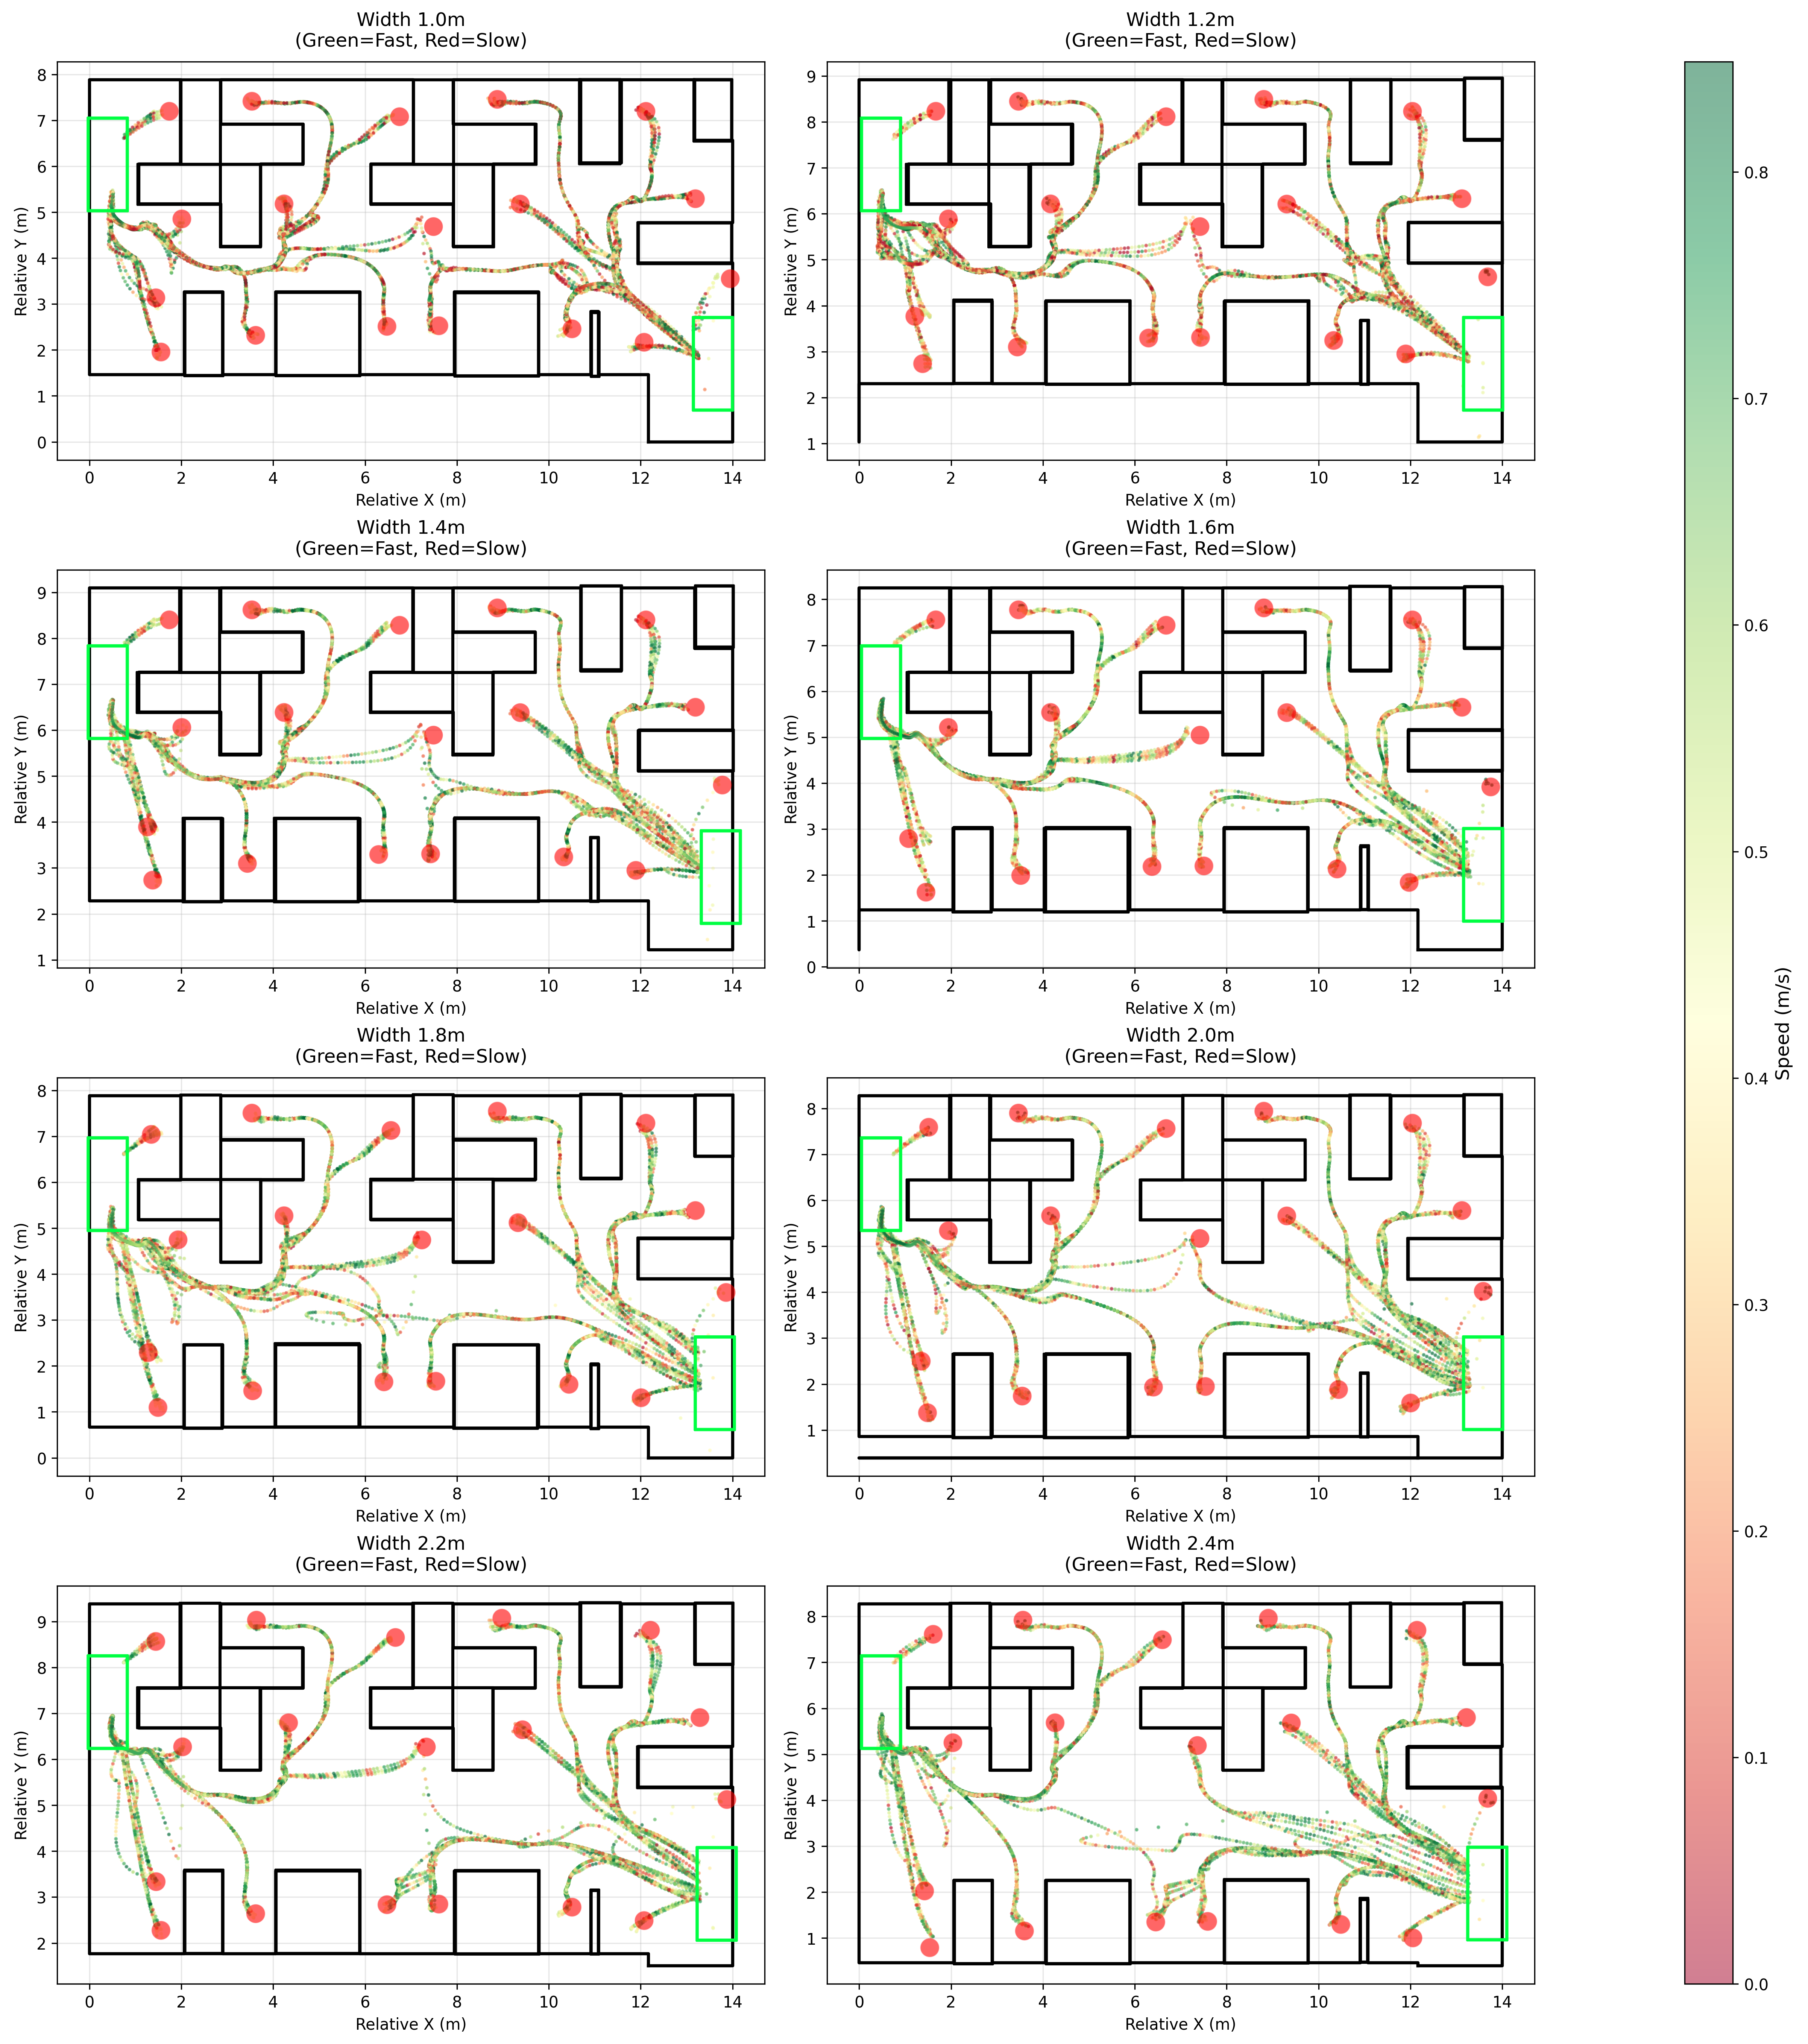
\includegraphics[width=\linewidth]{speed_trajectory_layout_B2.png}
    \caption{Speed and Trajectories for Layout B2}\label{fig:speed_trajectory_layout_B2}
\end{figure}

In single-exit Layout C \ref{fig:speed_trajectory_layout_C}, the parallel chnnels in the upper zone can form orderly queues in advance, but continuous low-speed zones appear at the corner. After setting up double exits \ref{fig:speed_trajectory_layout_C2}, the queues formed in the upper zone can be released directly through the upper-left exit without needing to pass through the corner and merge into the main corridor. This allows the Layout C2 to have the lowest overall evacuation time across all widths. This indicates that the double exits effectively weakened the influence of corner and fully utilized the advantages of parallel channels.

\begin{figure}[h]
    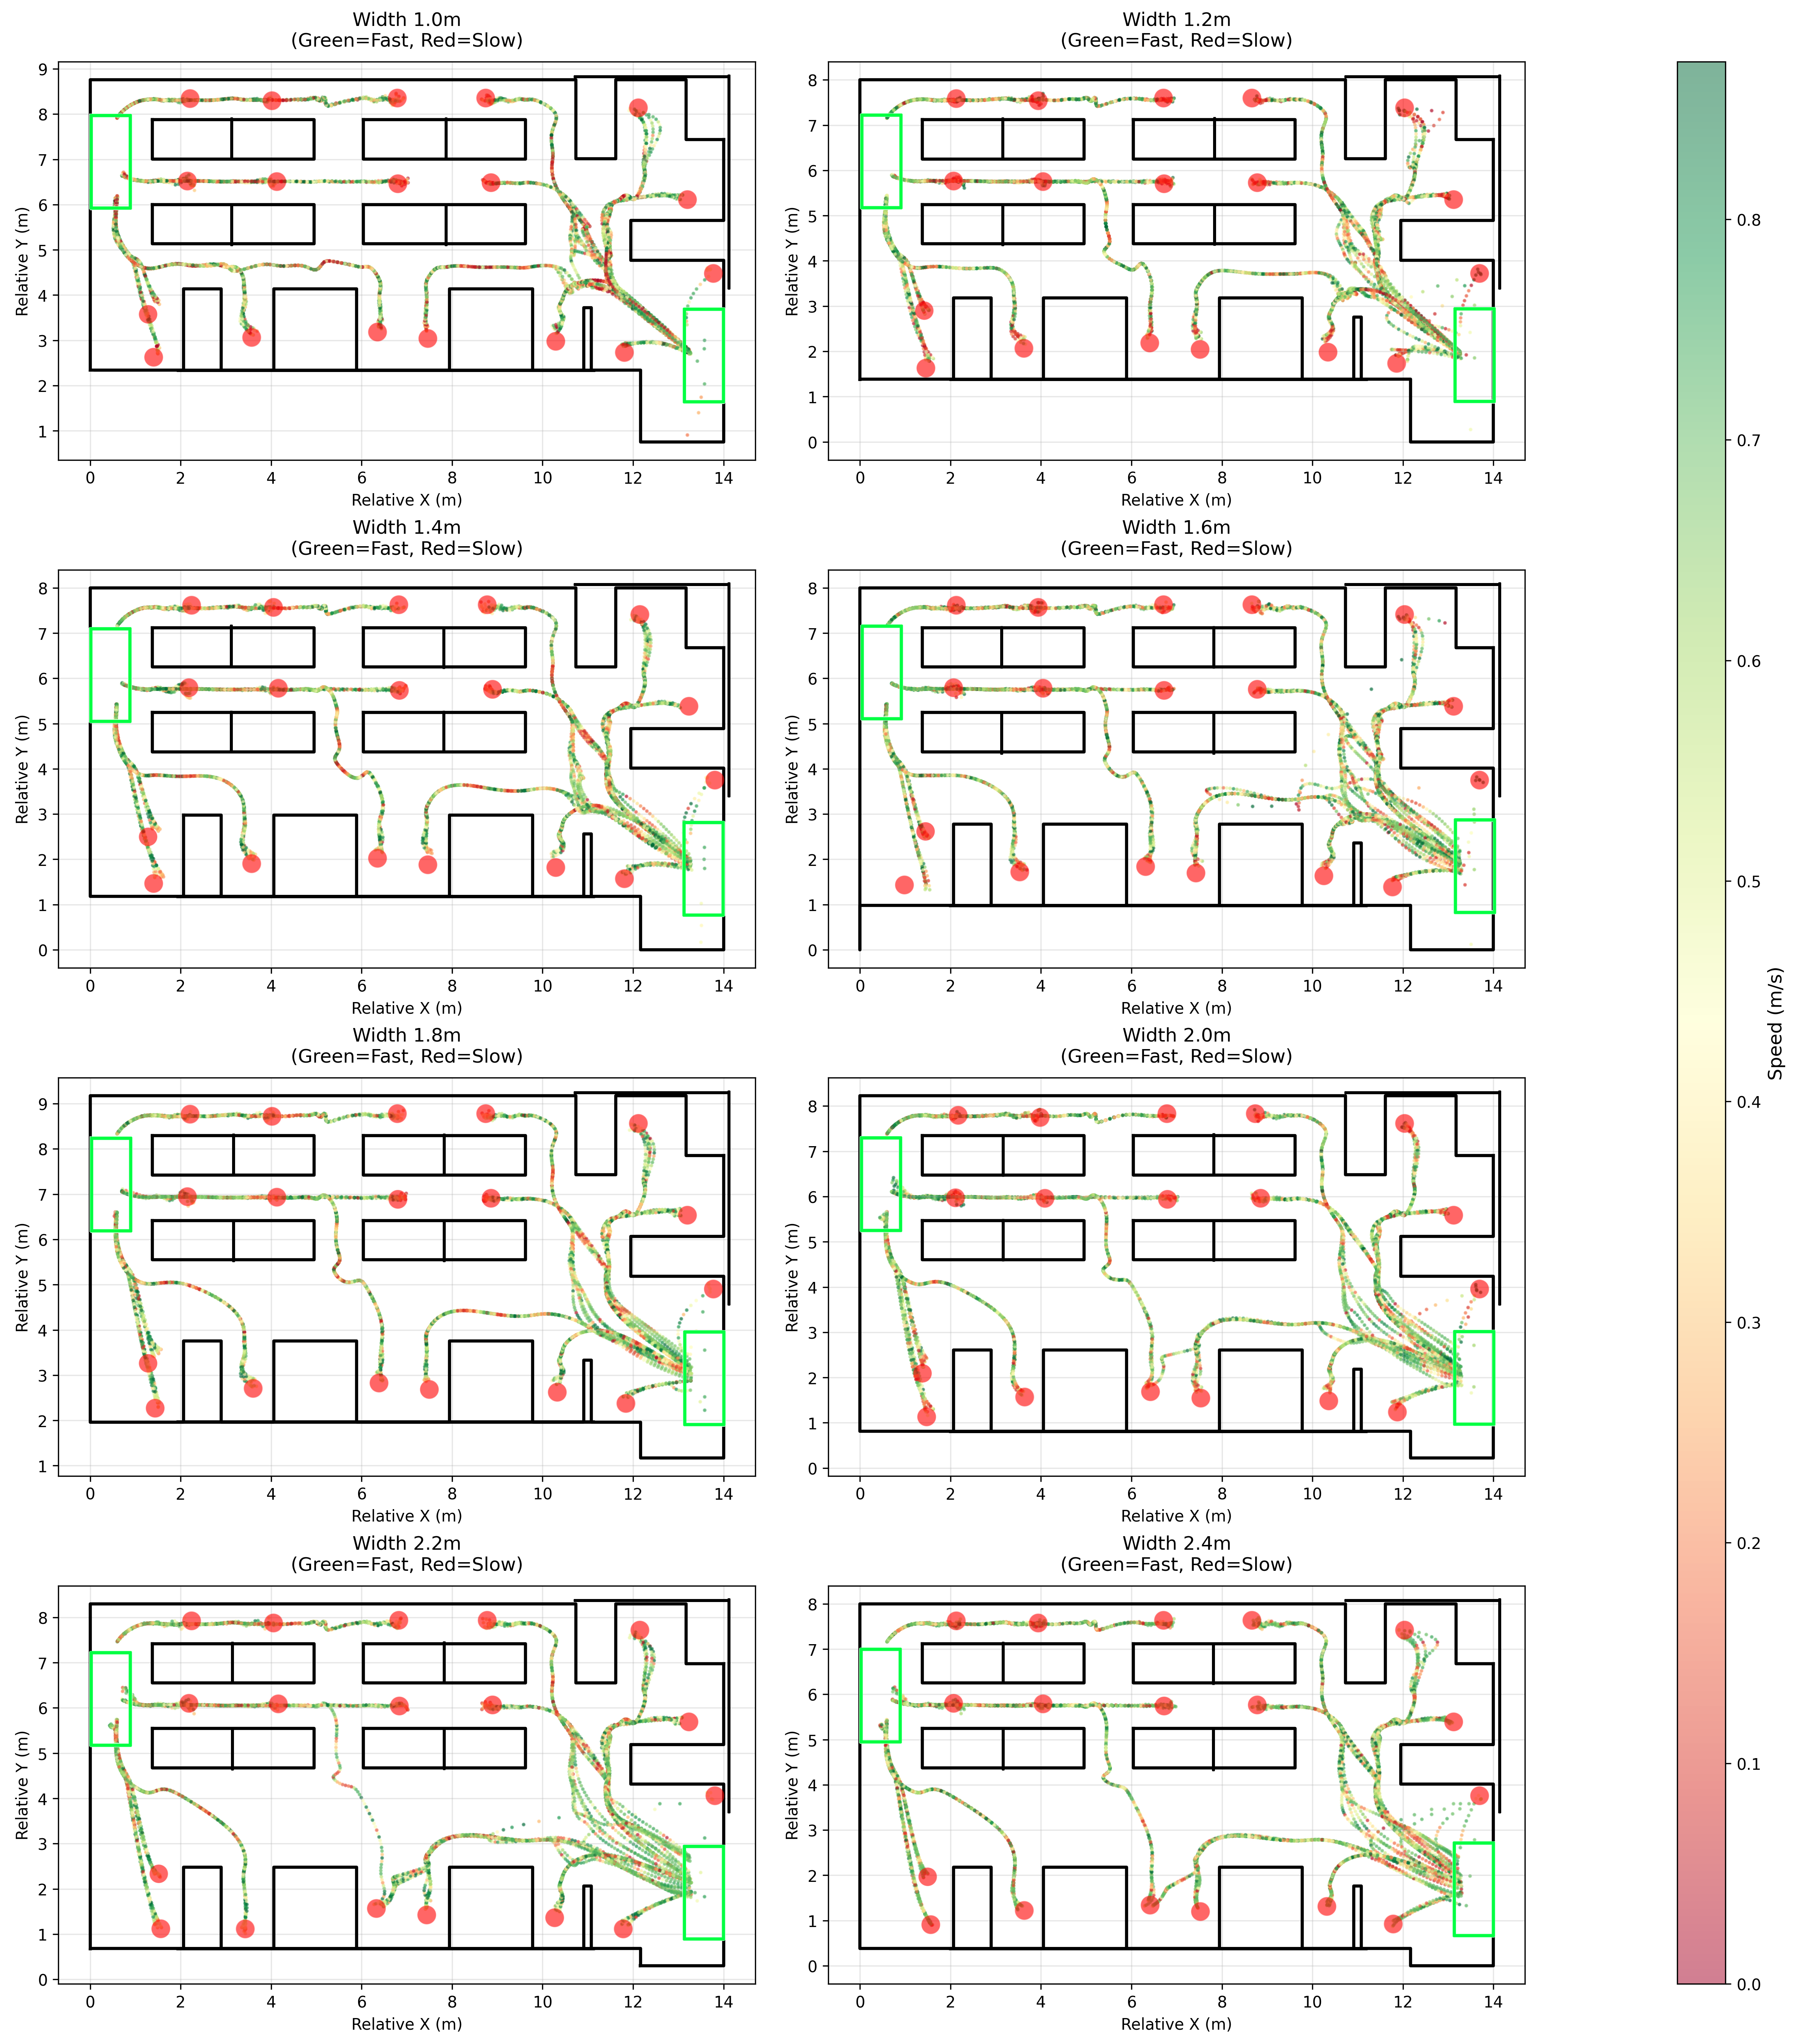
\includegraphics[width=\linewidth]{speed_trajectory_layout_C2.png}
    \caption{Speed and Trajectories for Layout C2}\label{fig:speed_trajectory_layout_C2}
\end{figure}

\section{Big Prototype}

Based on the results from the Small Prototype, evacuation time shows significant correlation with the convergence intensity at the end of main corridors, as well as mutual interference among crowds at intersections and merging points. Therefore, we introduce the Big Prototype to test these mechanisms in larger spaces and crowd scales, to examine their persistence and increase effects at the macro level, with focus on identifying the gates width and geometric threshold ranges that can most significantly infuence the TET.

\subsection{Effect of Bottleneck Width(Gate Width Before Exit)}

In the Big Prototype scenario, according to the figure \ref{fig:tet_vs_Bottleneck}, as the exit bottleneck width gradually increased from 1.0 m to 1.6 m, the TET showed a continuous declining monotonic trend. The readings approximately showed 85 s at 1.0 m, 75 s at 1.2 m, 73 s at 1.4 m, and 70 s at 1.6 m. The most significant improvement occurred in the interval from 1.0 m to 1.2 m, where TET decreased by approximately 10 s with nearly a twelve percent relative improvement; thereafter, continued widening only brought gradual improvements, with approximately 2 s reduction in the 1.2 m to 1.4 m interval and approximately 3 s reduction in the 1.4 m to 1.6 m interval. Error bars showed that the variability of repeated runs was greater at narrower exits and significantly converged at wider exits, indicating that the system was more stable at larger widths. The slope of the line showed a noticeable change around 1.2 m, suggesting that this point may be the threshold interval for transitioning from long queue formation to short-term congestion, beyond which marginal benefits gradually diminish.

\begin{figure}[h]
    \centering
    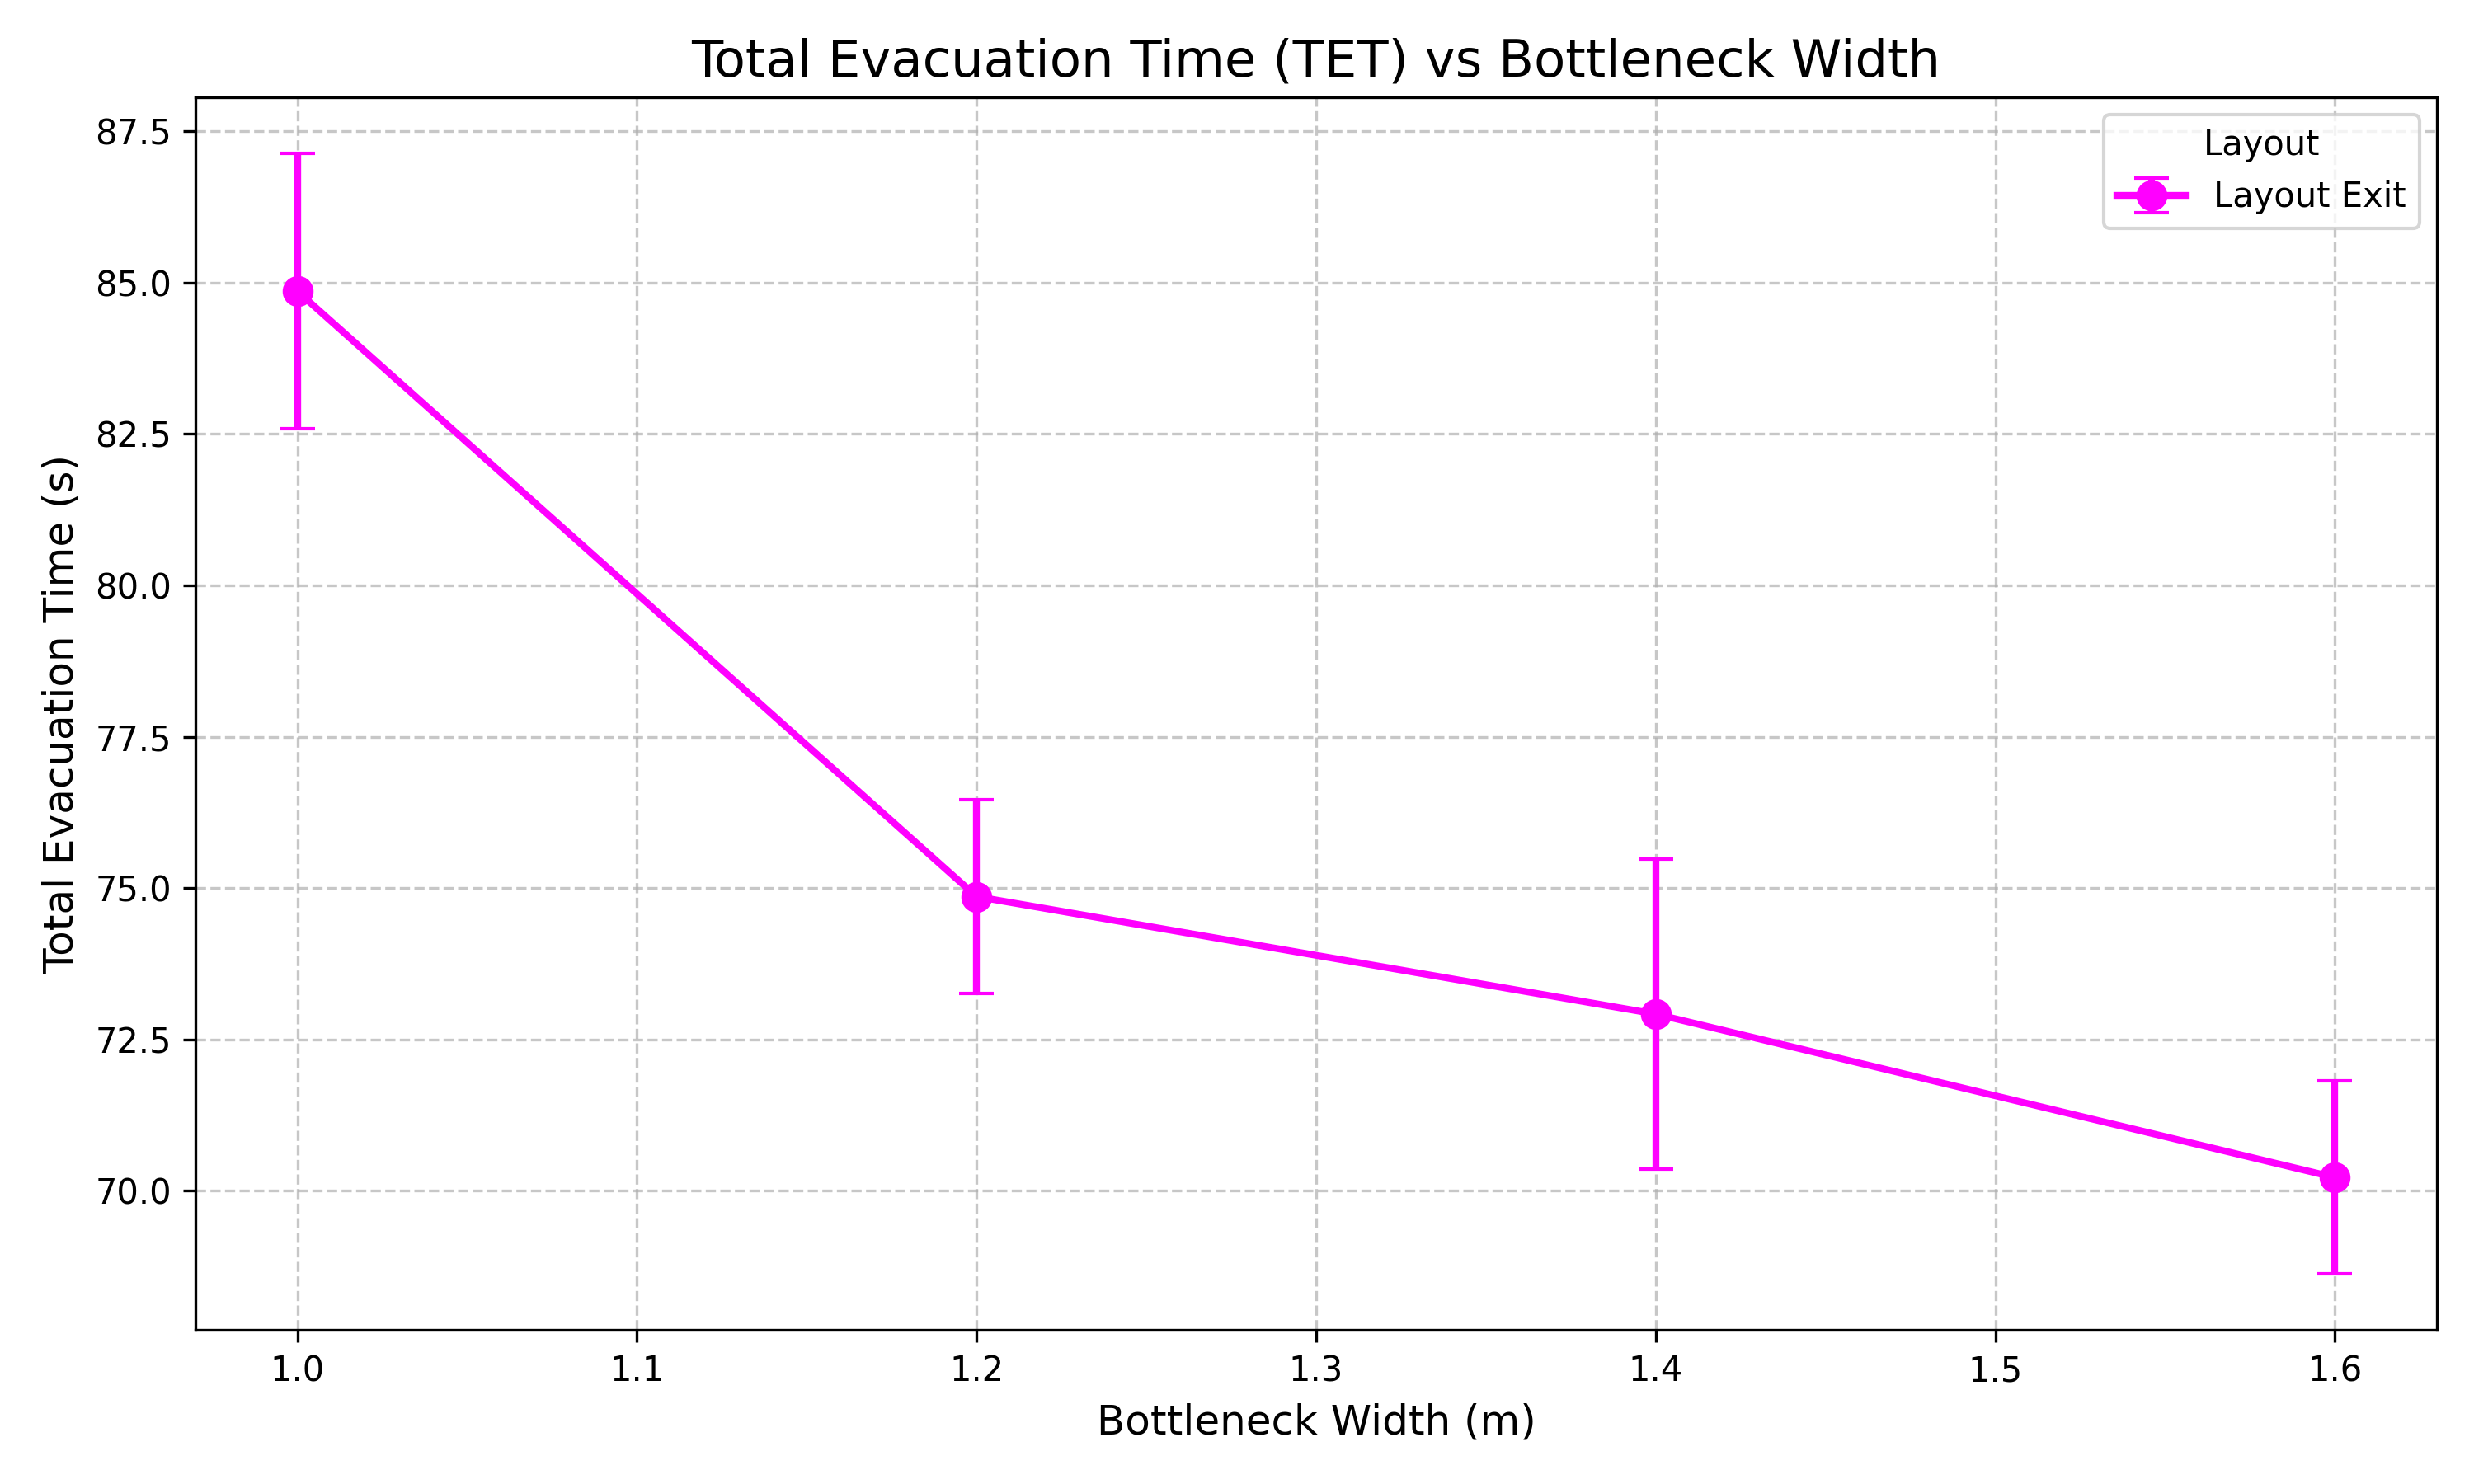
\includegraphics[width=\textwidth]{tet_vs_Bottleneck.png}
    \caption{TET vs Bottleneck Width}
    \label{fig:tet_vs_Bottleneck}
\end{figure}

The speed trajectory diagrams are consistent with the aforementioned trends. At the bottleneck width of 1.0 m \ref{fig:speed_trajectory_layout_1.0m}, the low-speed red zones significantly extend backward, showing queuing phenomena. Due to the queuing phenomenon, agents exhibit obvious convergence behavior at an early stage, beginning to merge lanes with frequent lateral interactions and substantial velocity fluctuations. When the width increases to 1.2 m \ref{fig:speed_trajectory_layout_1.2m}, the low-speed zone noticeably diminishs and becomes concentrated within several meters of the room exits, as well as the merging points be closer to the room exit. The agents' queuing phenomenon visibly disappears during actual simulation observation. On expansion to 1.4 m \ref{fig:speed_trajectory_layout_1.4m} and 1.6 m \ref{fig:speed_trajectory_layout_1.6m} , the low-speed zone continues to diminish and remains close to the doorway, with only brief delays occurring during peak arrival periods, more uniform velocity distribution, and reduced lateral conflicts. The multiple simulations show that the main corridor and overall paths leading to each exit remain consistent, while width variations not triggering large-scale route diversions. The most significant differences are concentrated in the flow microstructure within the final several meters of the exit area.

\begin{figure}[h]
    \centering
    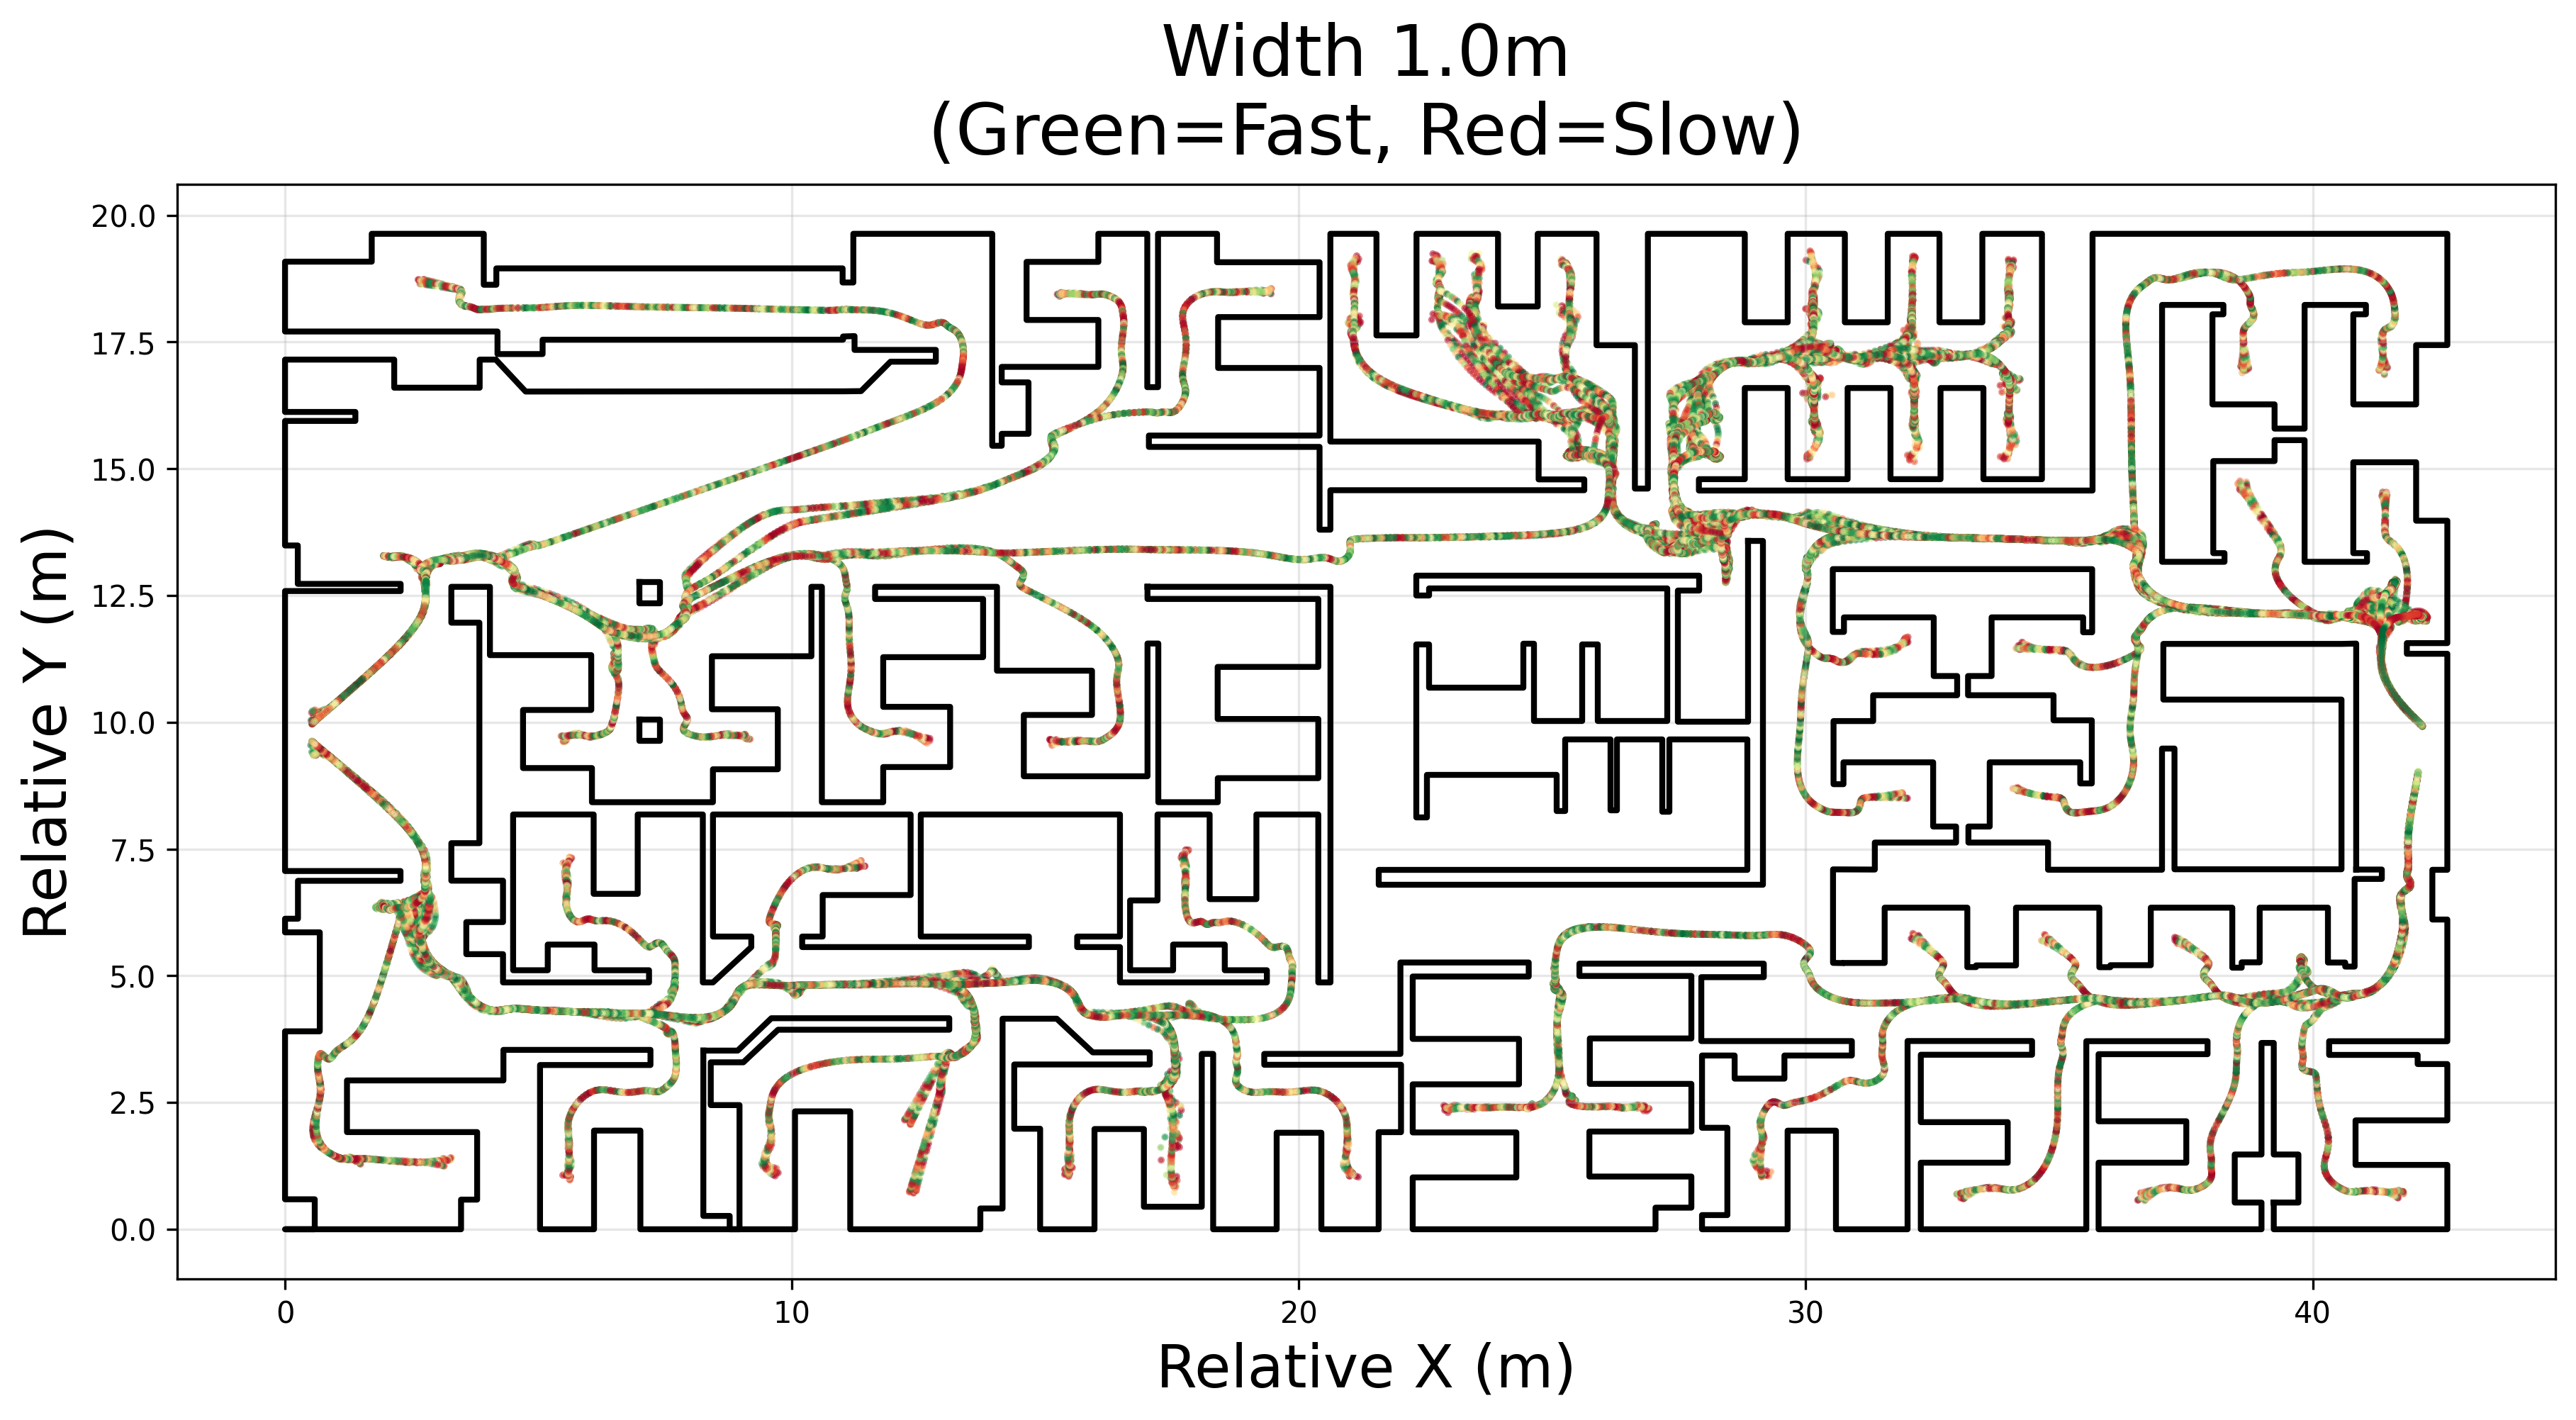
\includegraphics[width=\textwidth]{speed_trajectory_Exit_width_1.0m.png}
    \caption{Speed and Trajectories for 1.0m Bottleneck Width}
    \label{fig:speed_trajectory_layout_1.0m}
\end{figure}

\begin{figure}[h]
    \centering
    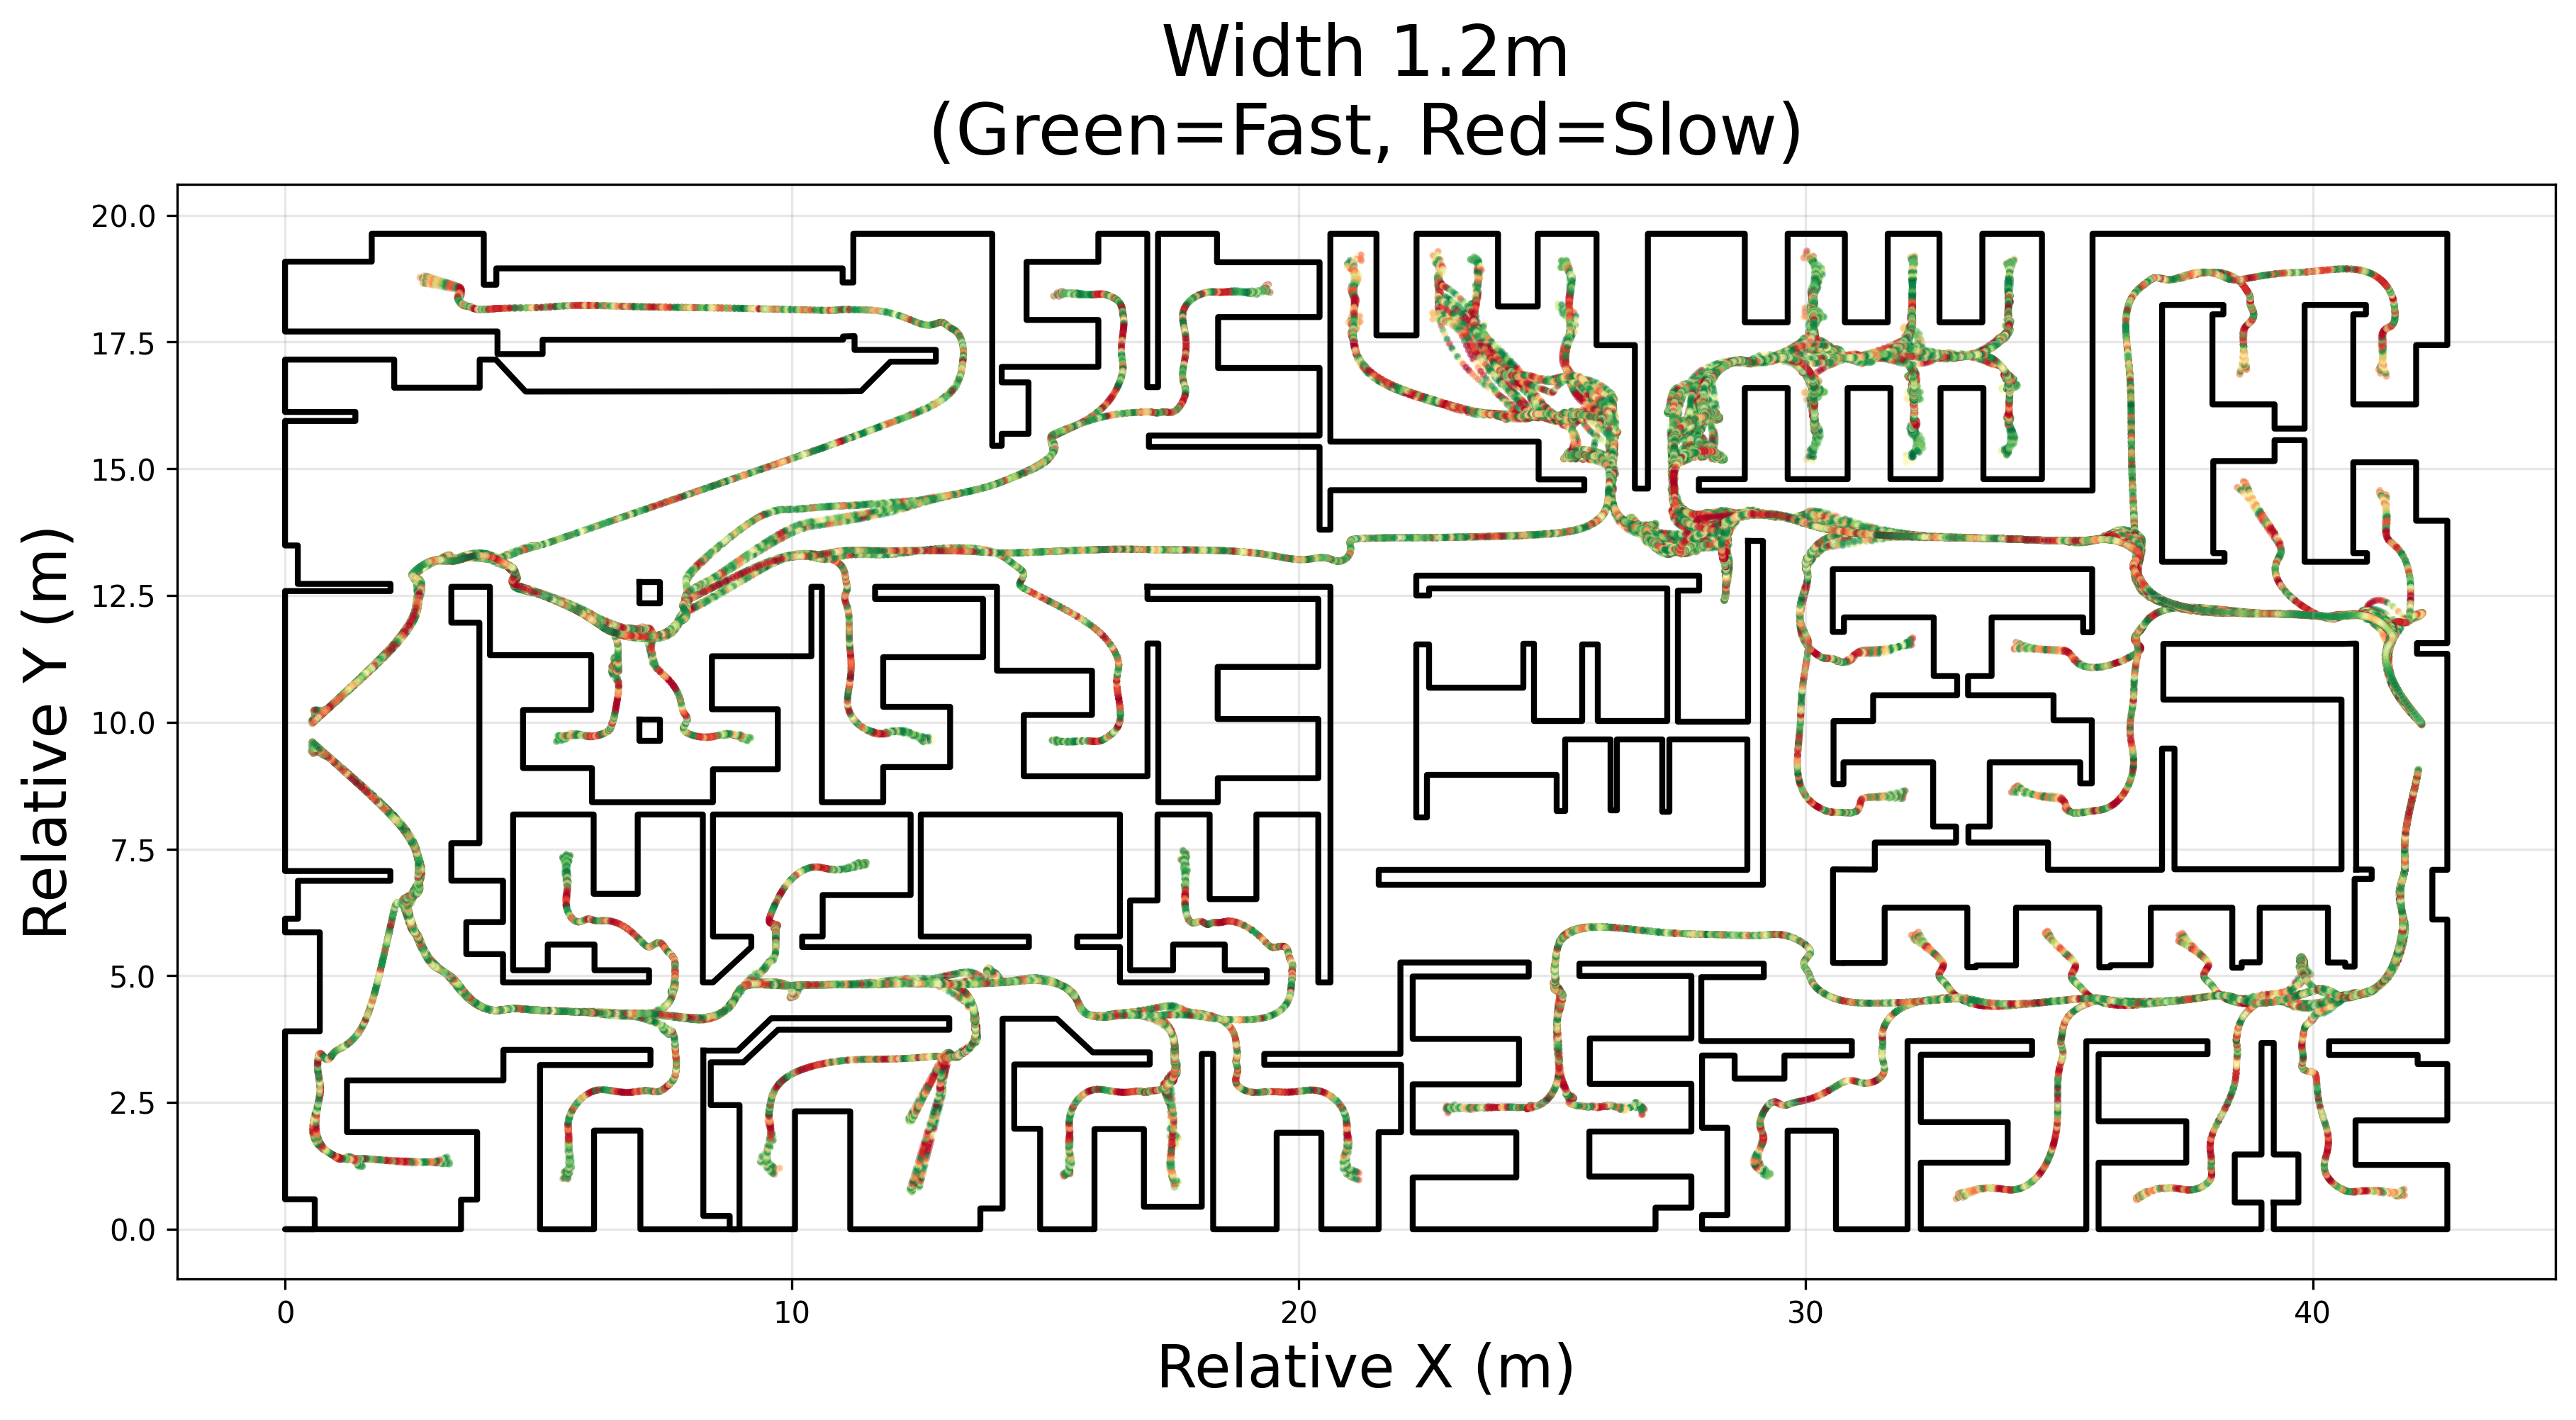
\includegraphics[width=\textwidth]{speed_trajectory_Exit_width_1.2m.png}
    \caption{Speed and Trajectories for 1.2m Bottleneck Width}
    \label{fig:speed_trajectory_layout_1.2m}
\end{figure}

\begin{figure}[h]
    \centering
    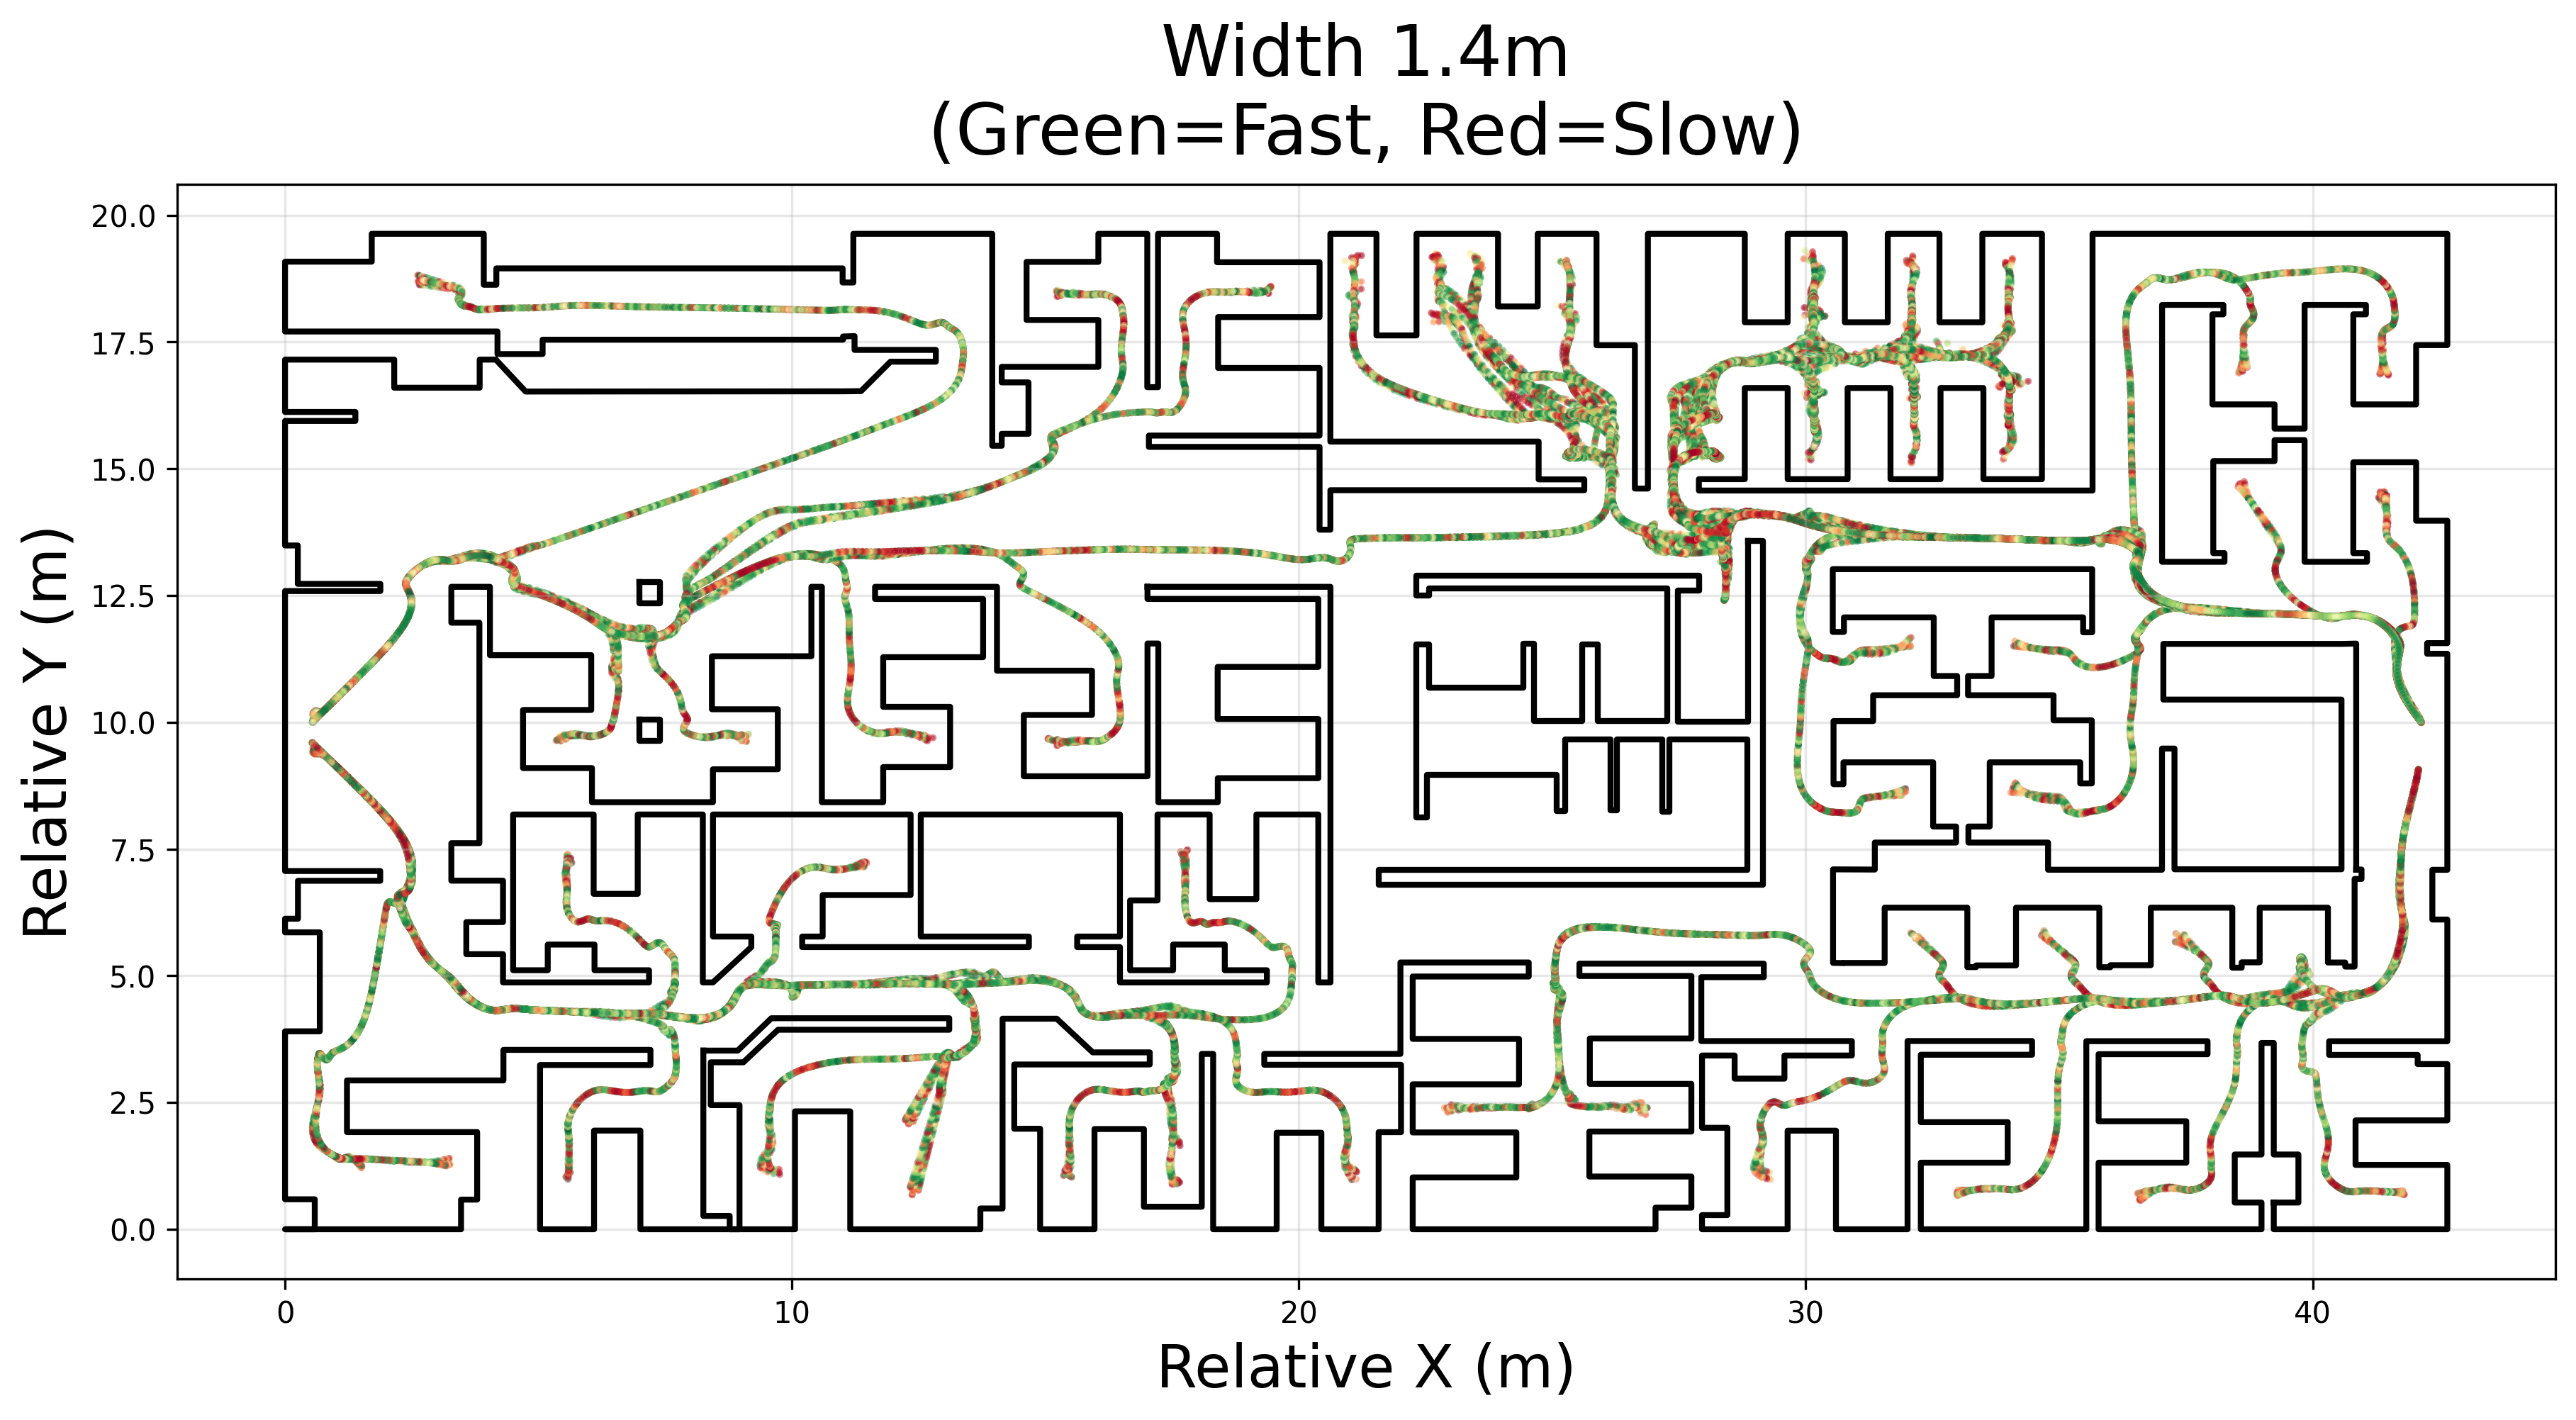
\includegraphics[width=\textwidth]{speed_trajectory_Exit_width_1.4m.png}
    \caption{Speed and Trajectories for 1.4m Bottleneck Width}
    \label{fig:speed_trajectory_layout_1.4m}
\end{figure}

\begin{figure}[h]
    \centering
    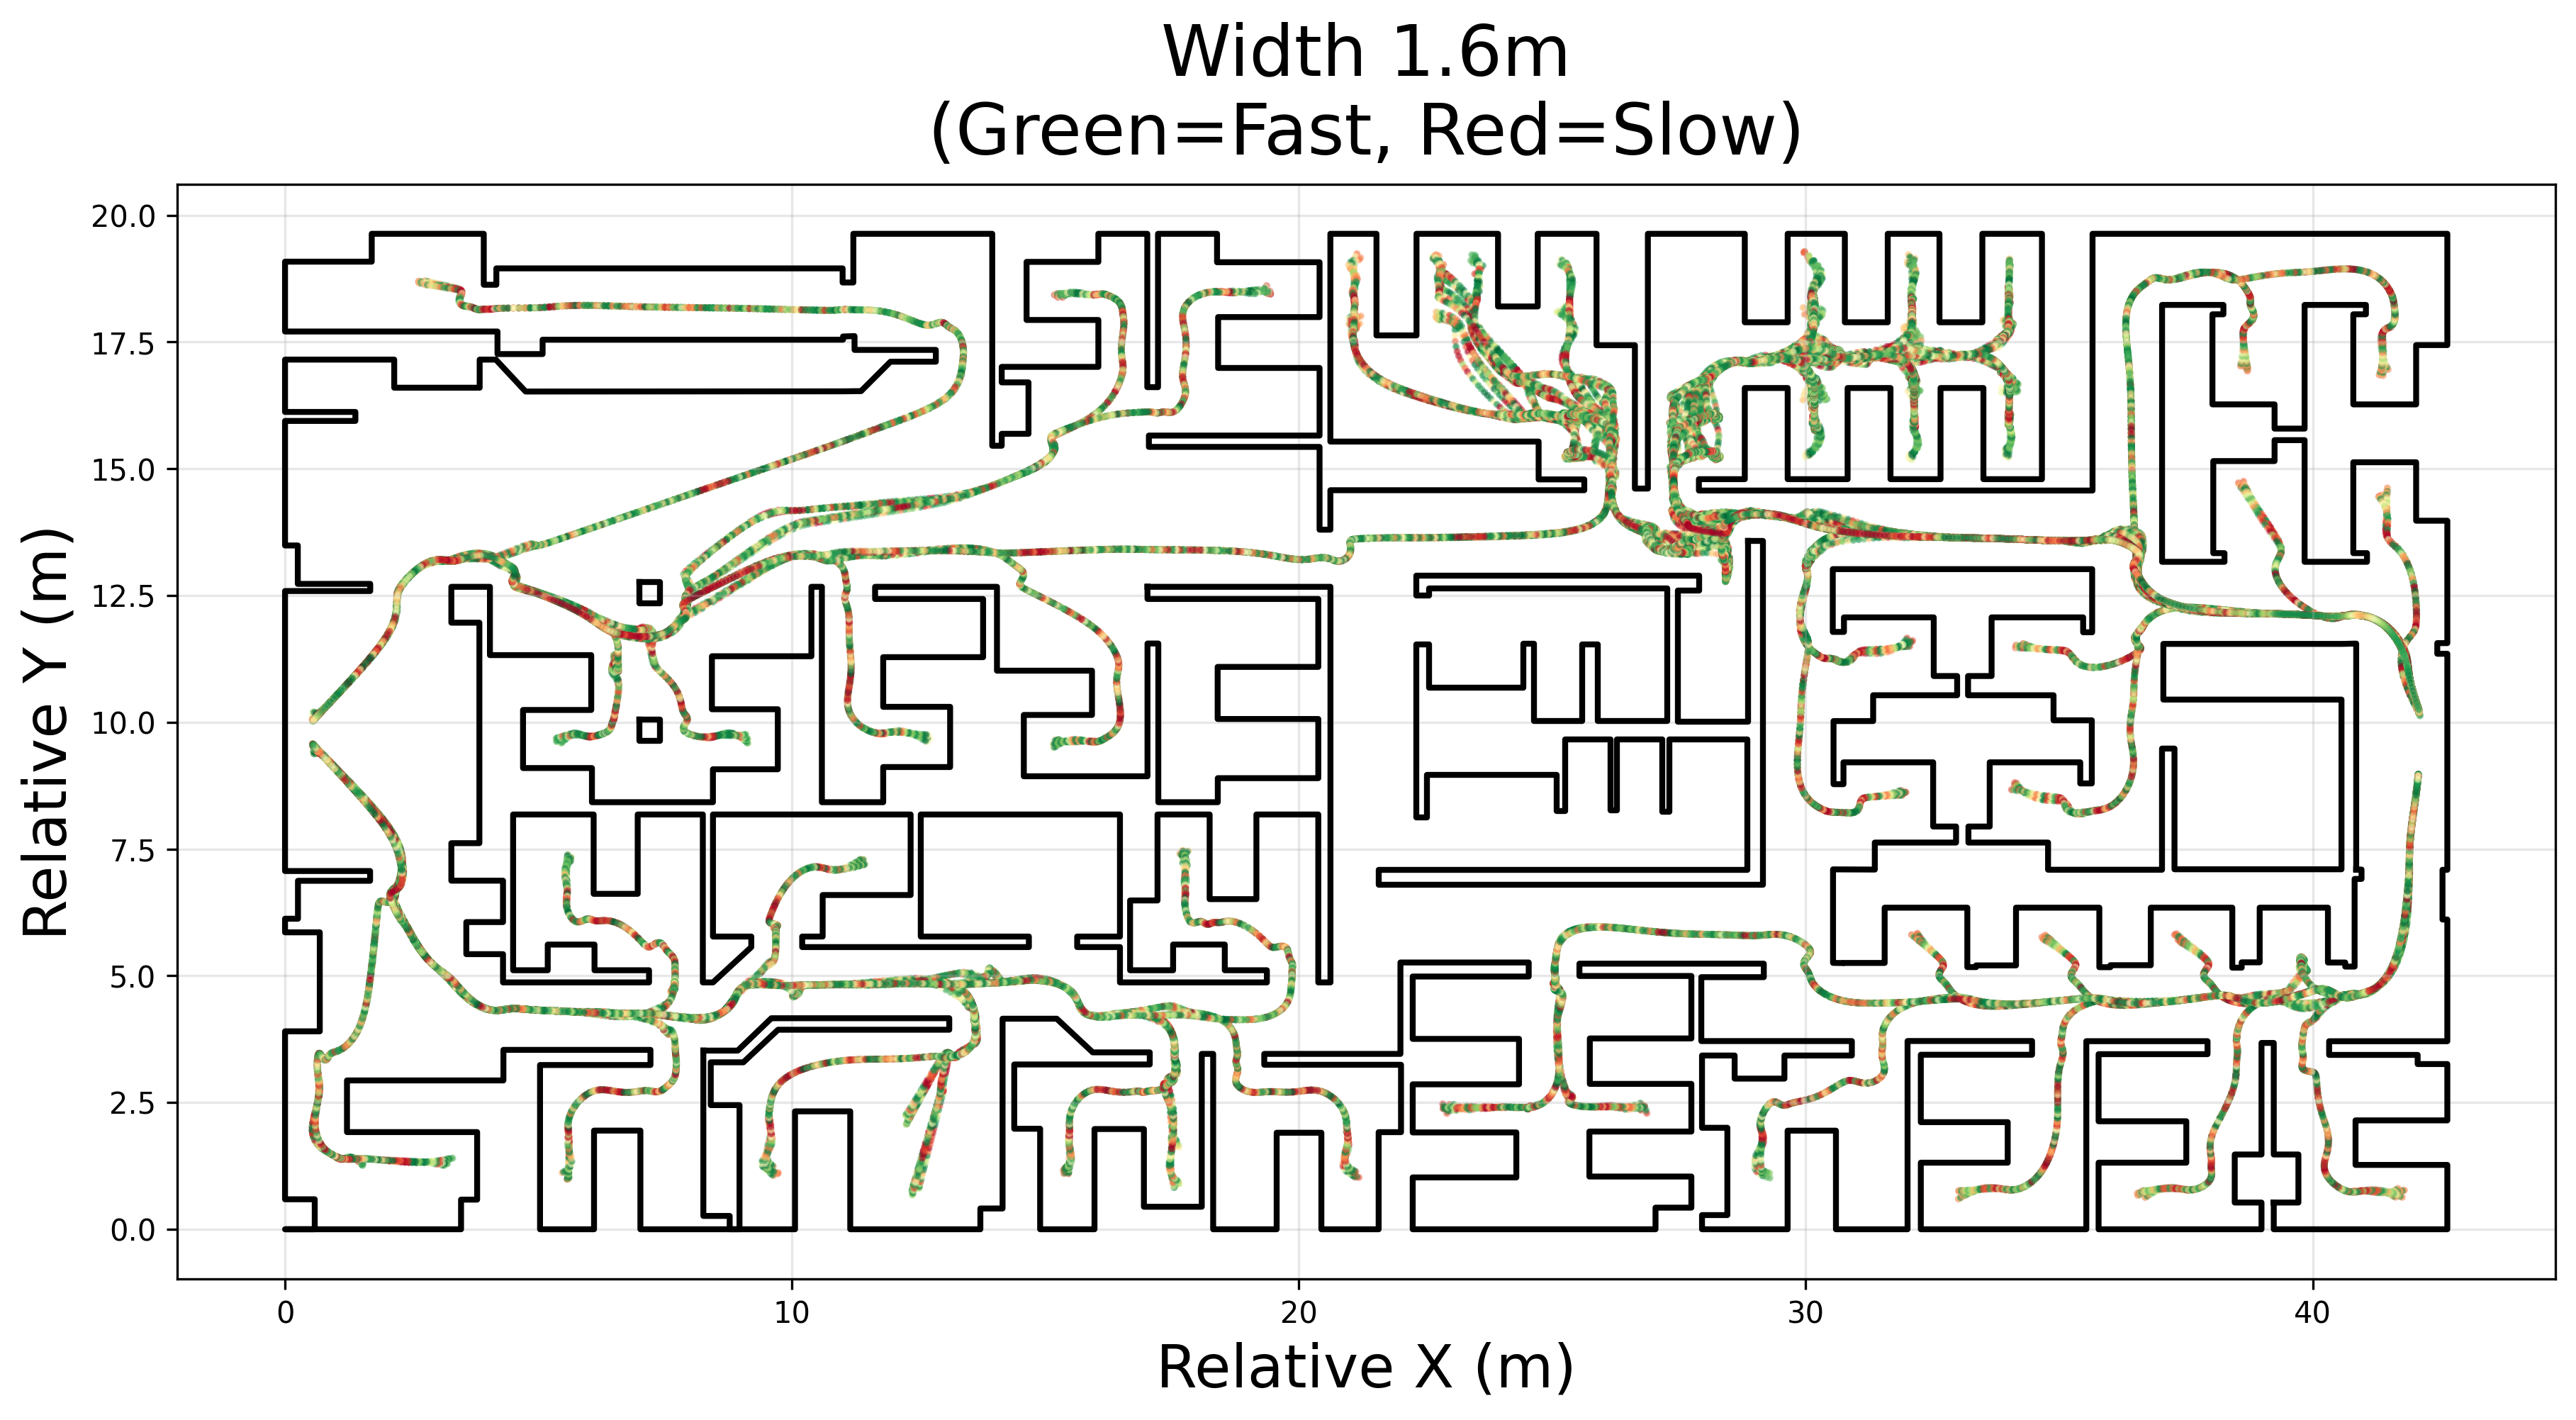
\includegraphics[width=\textwidth]{speed_trajectory_Exit_width_1.6m.png}
    \caption{Speed and Trajectories for 1.6m Bottleneck Width}
    \label{fig:speed_trajectory_layout_1.6m}
\end{figure}

The overlapping trajectories illustrate that the main path remains relatively stable across all widths, with only slight differences showed up in the congestion before the exit. Corresponding to the performance of TET error bars, the run results under wider gate conditions are more concentrated, indicating that intermittent congestion in the exit vicinity is weakened, system behavior becomes more predictable, and the consistency of repeated experiments is also improved.

Based on the comprehensive evidence from both TET curves and velocity trajectory analysis, the main conclusions can be summarized in the following narrative. The most significant performance improvement occurred when increasing the bottleneck width from 1.0 m to 1.2 m, during which the queuing phenomenom disppeared, and the merging points approached the exit. Further widening to 1.4 m and 1.6 m continued to reduce TET, but with smaller improvements, mainly manifesting as further reduction of short-term low-speed conditions near the exit line.  These results provide direct support for subsequent design recommendations, with specific conclusions and suggestions to be presented in the Conclusion section.

\subsection{Coupling Effect of Corridor Entrance and Passage Gate Width}
Based on the experiments described in the last section, we selected 1.2m under simulated stable conditions as the standard bottleneck width parameter to test the coupling effect of room door width and corridor gate width, in order to minimize the conflicts and interference caused by bottlenecks as much as possible, thereby improving the system's robustness and accuracy.

According to the heat maps \ref{fig:tet_vs_room_corridor_coupling}, The horizontal axis represents corridor gate width, and the vertical axis represents room door width, with both parameters taking values of 1.0, 1.2, 1.4, and 1.6 m. For each combination, multiple independent simulations were conducted while maintaining agents numbers, layout, and model parameters. The mean and standard deviation of TET were calculated and presented as the color variation.

Among all combinations, the shortest TET was 69.7 s, which occurs when corridor width is 1.4m and room door width is 1.2m. The longest TET was 89.5 s, showing when corridor width is 1.0m and room door width is 1.4m. When corridor gate width increased to 1.4 m and above, the TET for all combinations clearly converged to approximately 70-72 s, with standard deviations generally decreasing to about 1-2 s, indicating that the system is getting stable. Especially significant is that when the corridor gates were narrow (1.0 or 1.2 m), increasing room door width alone significantly slowed evacuation time. This phenomenon is consistent with merging conflicts and queue backtracking observed in speed-trajectory diagrams, and this mechanism will be further explained in conjunction with speed-trajectory diagrams in subsequent paragraphs.

\begin{figure}[h]
    \centering
    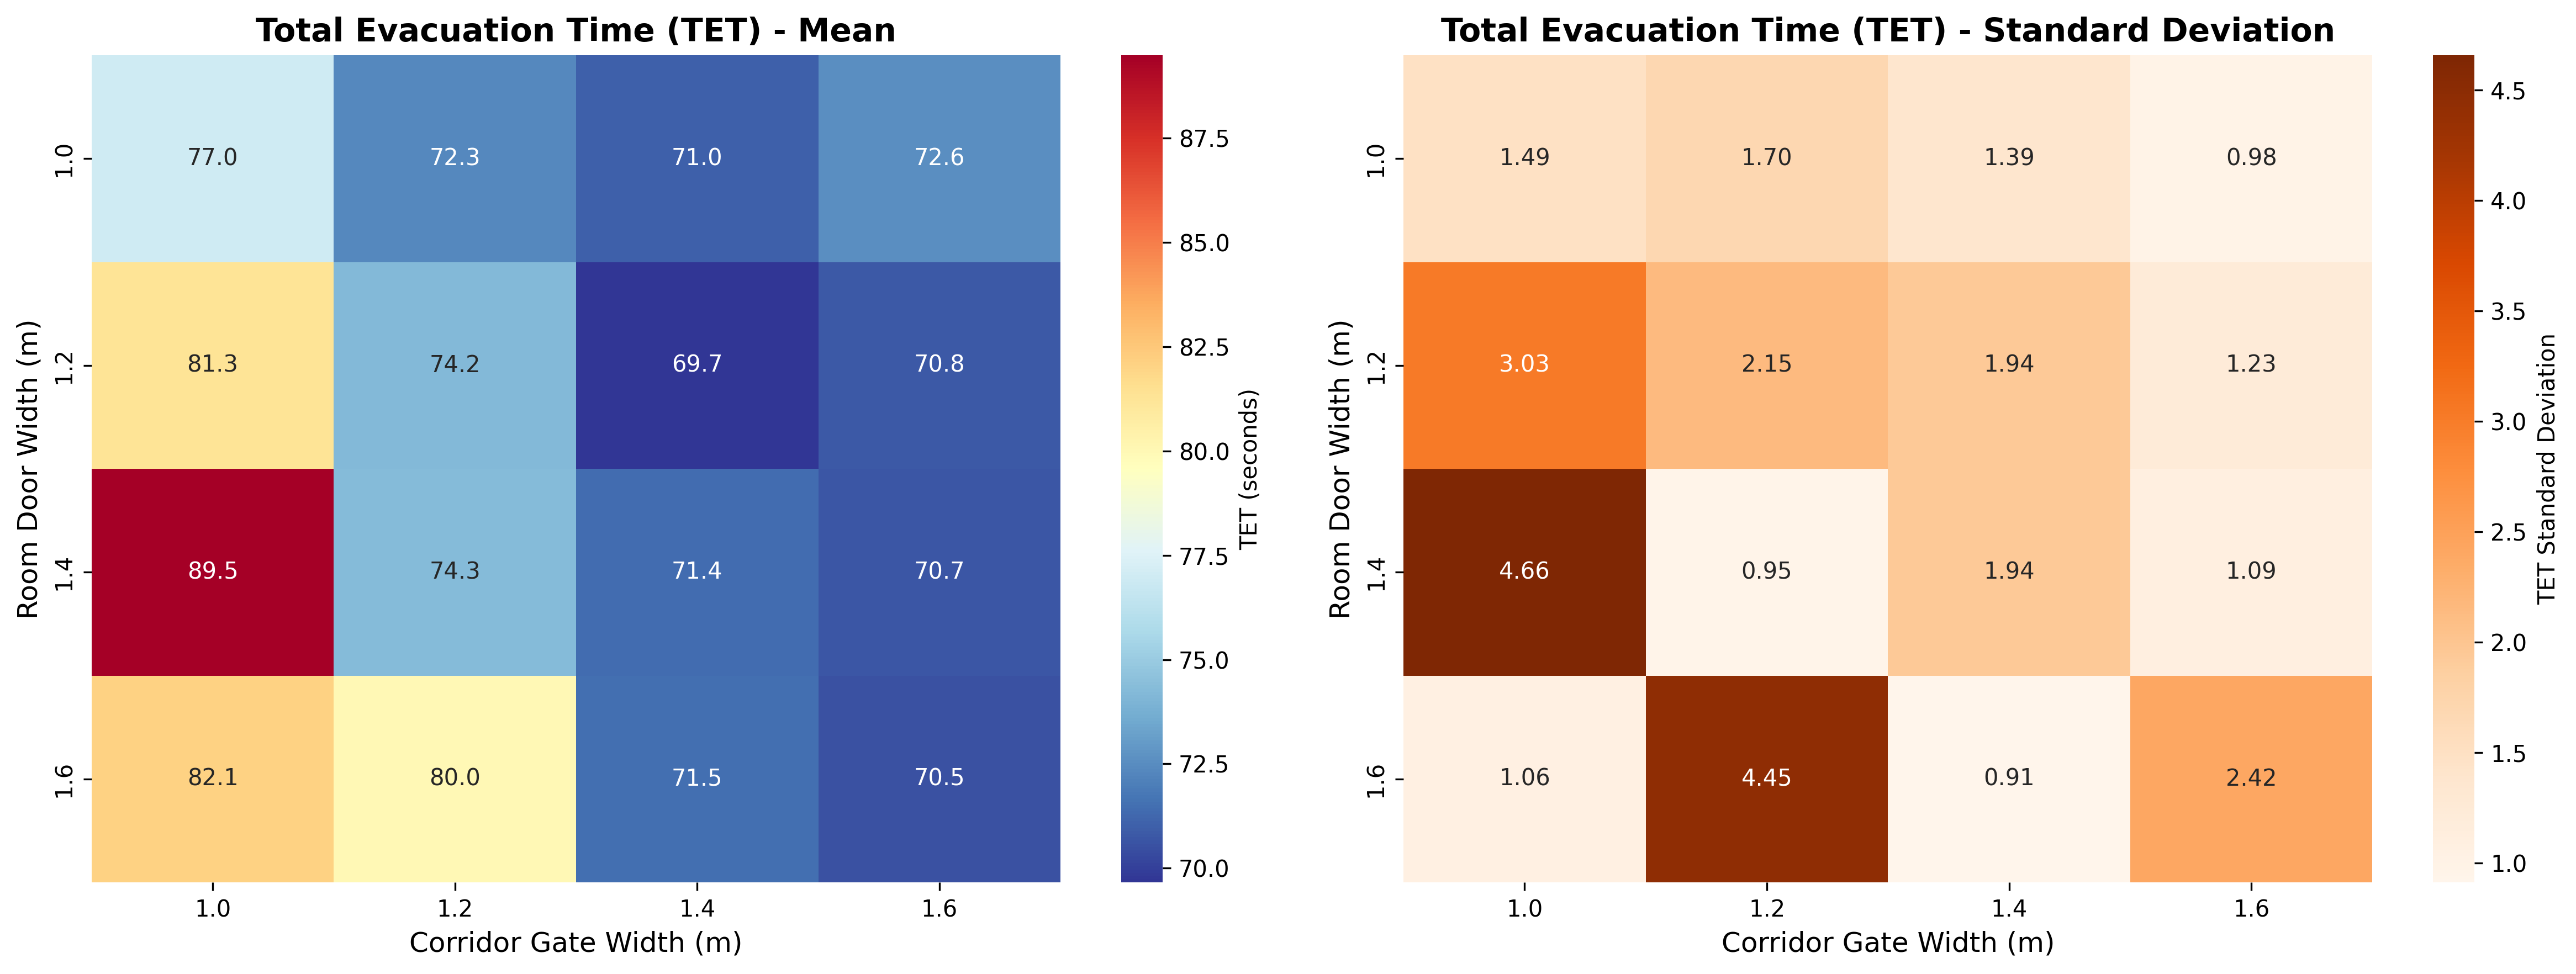
\includegraphics[width=\textwidth]{tet_seaborn_heatmap_multiroom.png}
    \caption{TET vs Room-Corridor Coupling}
    \label{fig:tet_vs_room_corridor_coupling}
\end{figure}

Figure \ref{fig:width_combo_1.0_x} shows that when room door width is 1.0m, the spatial distribution of congestion evolves as the corridor gate width gradually widens from 1.0m to 1.6m, and directly correspond to the changes in the mean TET and standard deviation of the first row of the heat map. Under the combo of 1.0m and 1.0m, large areas of low-speed zones appear near the main corridor and the merging points. Backtracking several meters upstream, this indicates frequent parallel conflicts, long and continuous queues, which precisely correspond to the relatively high evacuation time in the heat map. After increasing the corridor door to 1.2 meters, the red band shrank significantly. The slow points were mainly compressed at corners and threshold positions. The green continuous section on the main passage became longer, and the number of lane changes and confliction decreased. Therefore, the TET dropped down greatly. When further increased the door width to 1.4m, the slow zone continues to be close to the edge and shortens, forming a stable multi-lane queue near the convergence point. The passage almost no longer causes visible backtracking to the upstream, which is consistent with the heat map reaching the shortest time within the row in this column. When further widened to 1.6m, the trajectory shape is already very close to 1.4m. The low-speed points are scattered and limited to individual geometric corners. The system performance is more predictable, thereby resulting in a smaller standard deviation. Meanwhile, as the door remains the upper limit of the system's supply, the additional widening of the corridor door no longer leads to an increase in effective throughput. As a result, the average value only slightly rises from 1.4m, and the overall situation remains at the same stable level.

\begin{figure}[H]
    \centering
    \begin{subfigure}[b]{.45\linewidth}
        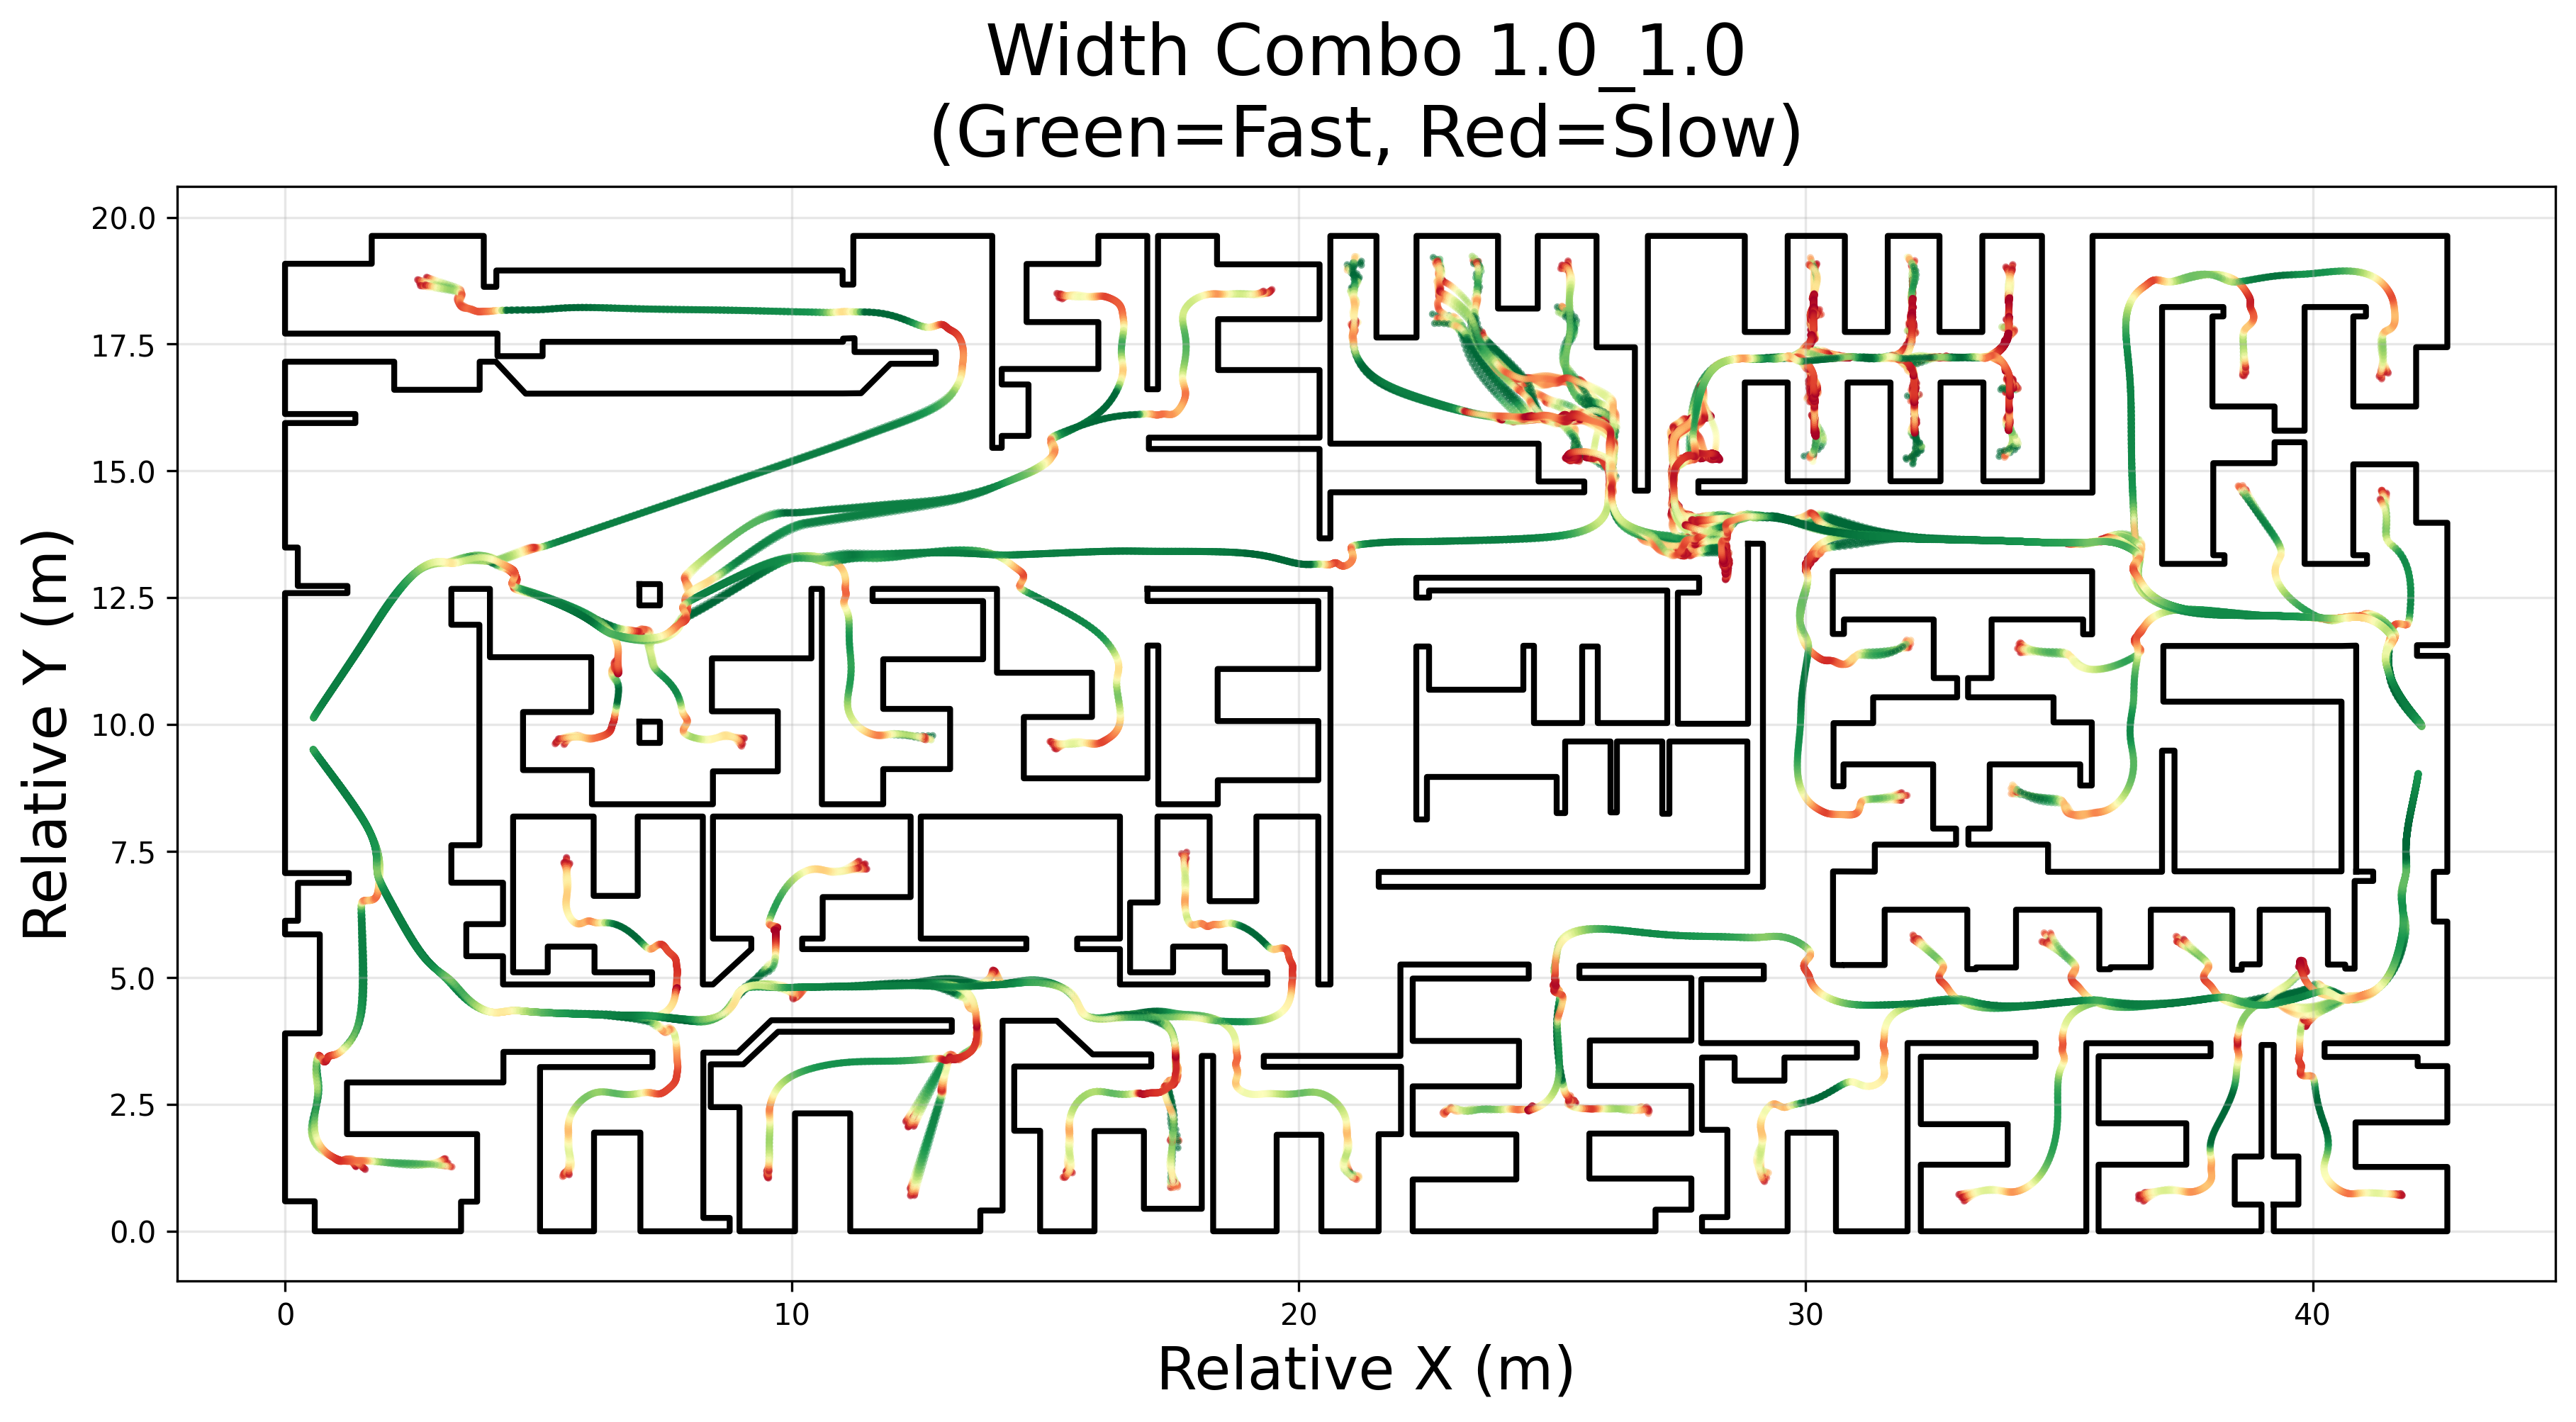
\includegraphics[width=\linewidth]
        {speed_trajectory_MultiRoom_width_1.0_1.0.png}
        \caption{Width Combo 1.0m and 1.0m}
        \label{fig:width_combo_1.0_1.0m}
    \end{subfigure}
    \begin{subfigure}[b]{.45\linewidth}
        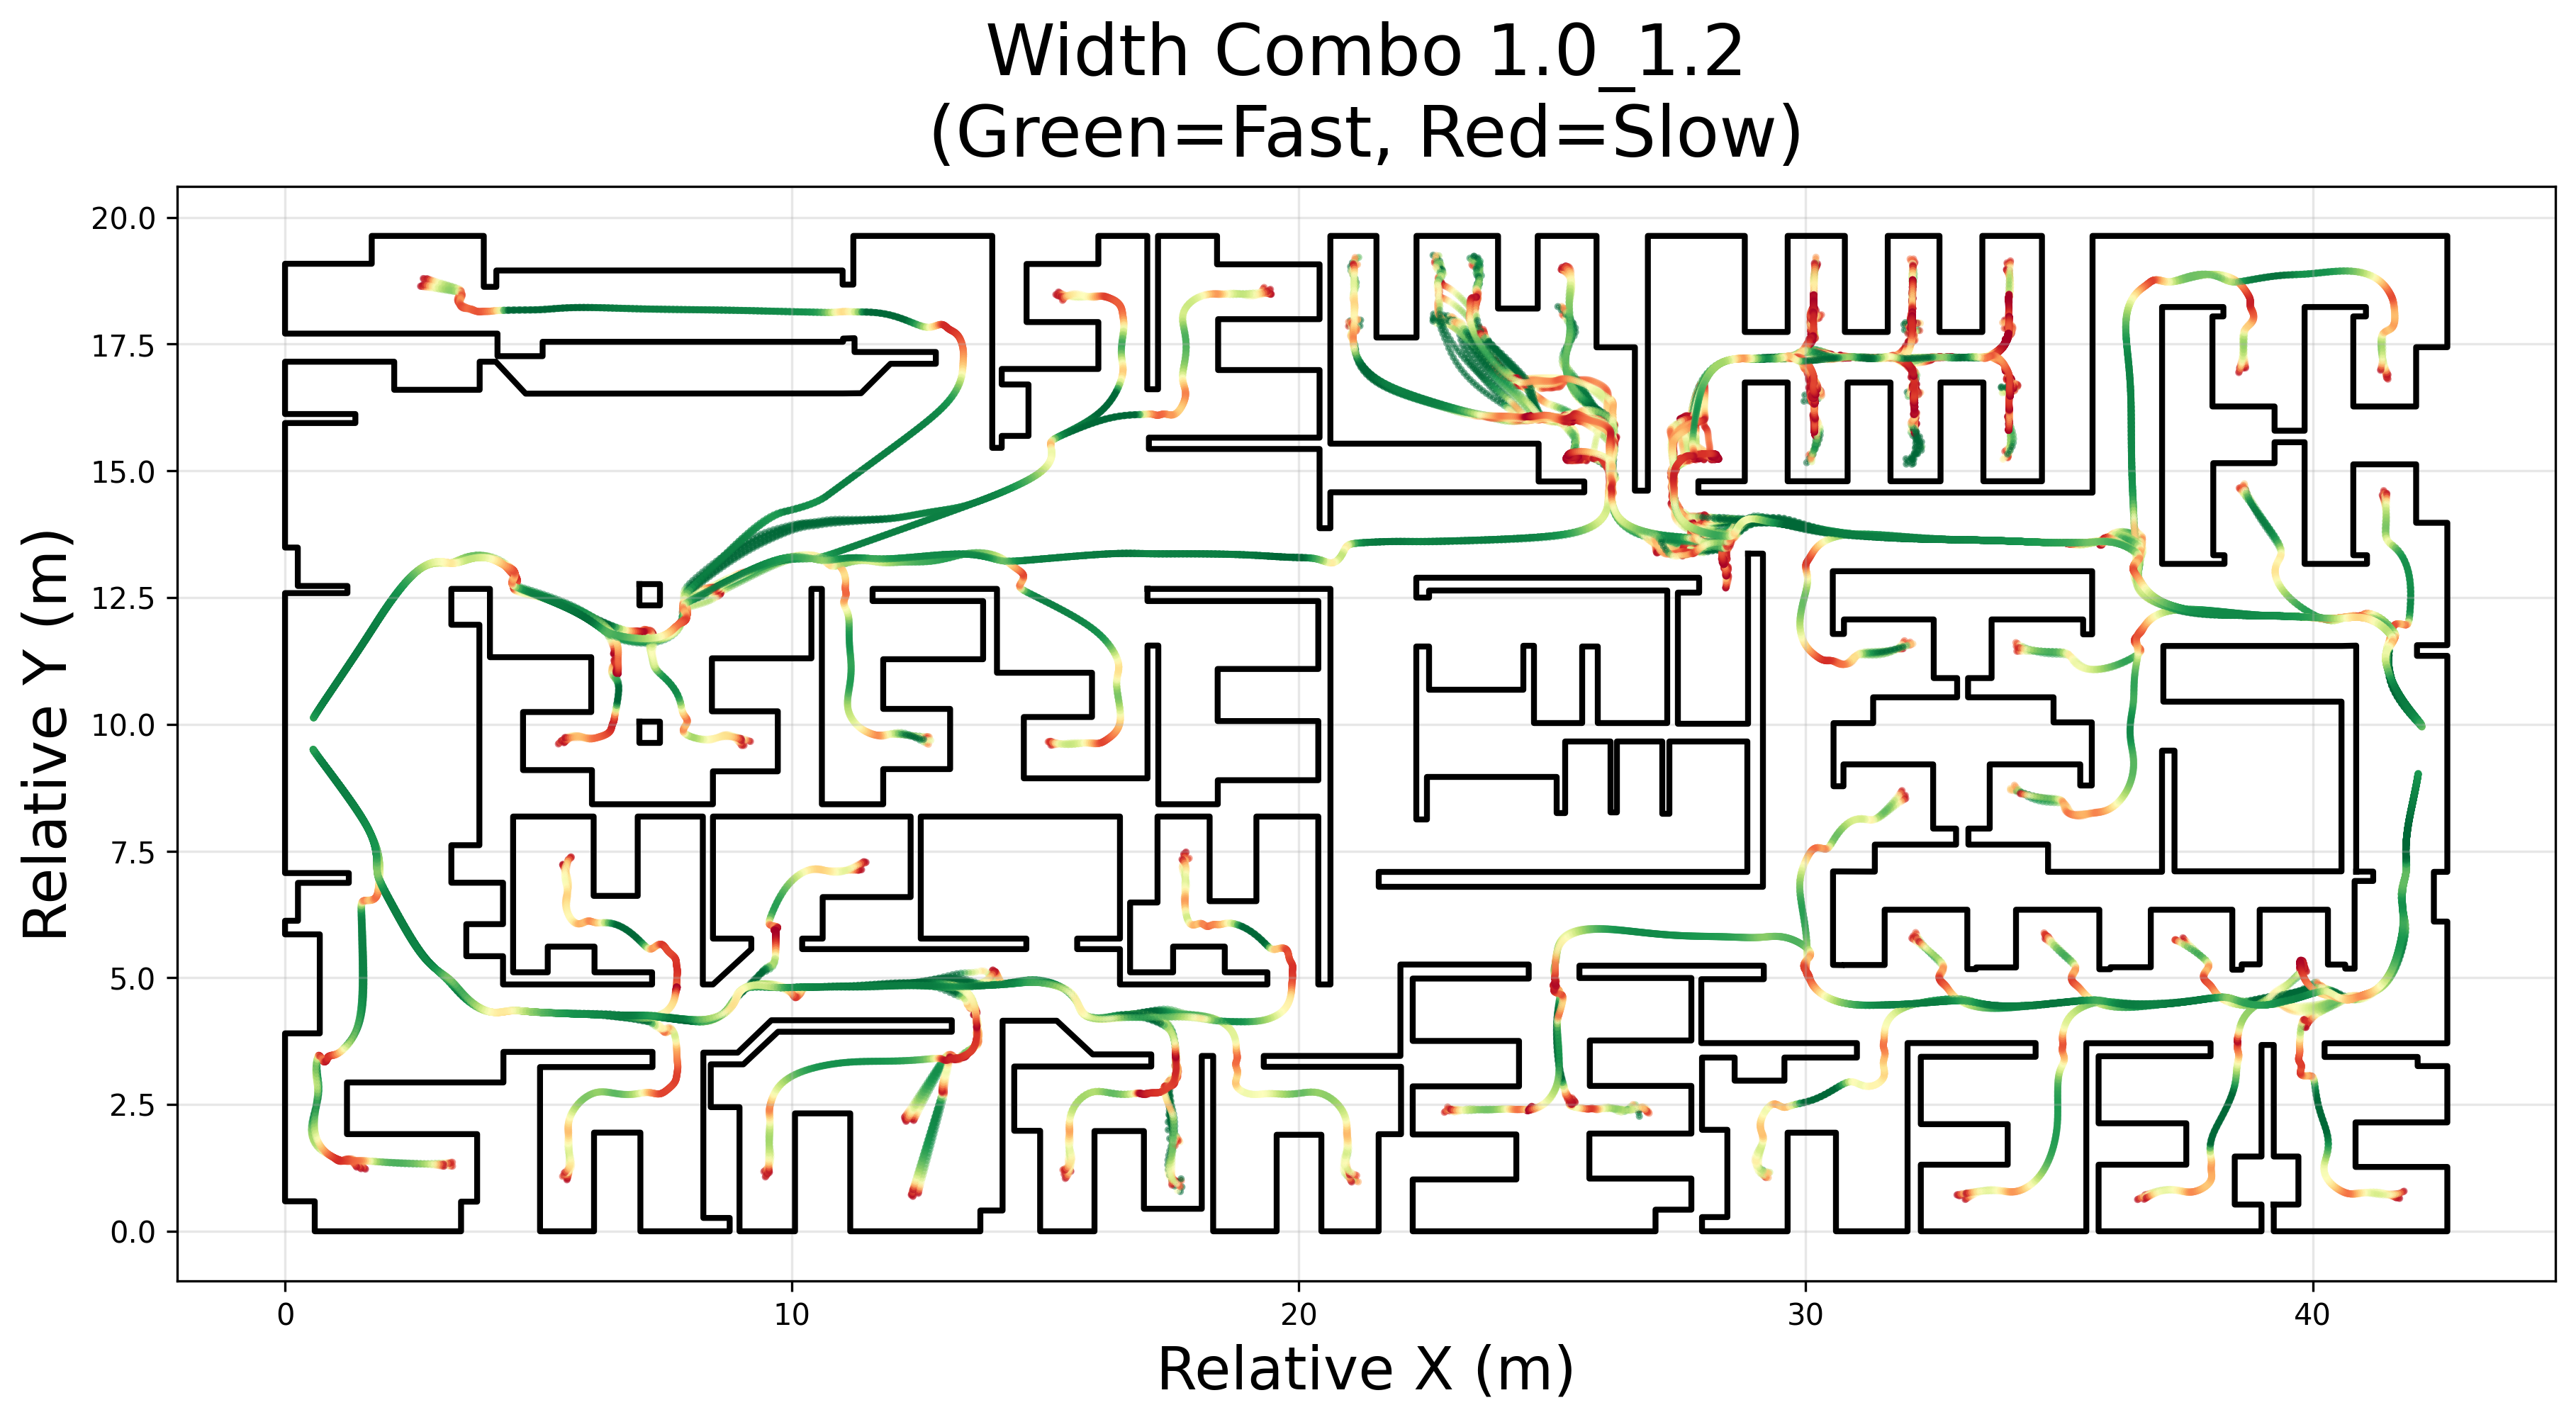
\includegraphics[width=\linewidth]{
            speed_trajectory_MultiRoom_width_1.0_1.2.png}
        \caption{Width Combo 1.0m and 1.2m}
        \label{fig:width_combo_1.0_1.2m}
    \end{subfigure}
    \begin{subfigure}[b]{.45\linewidth}
        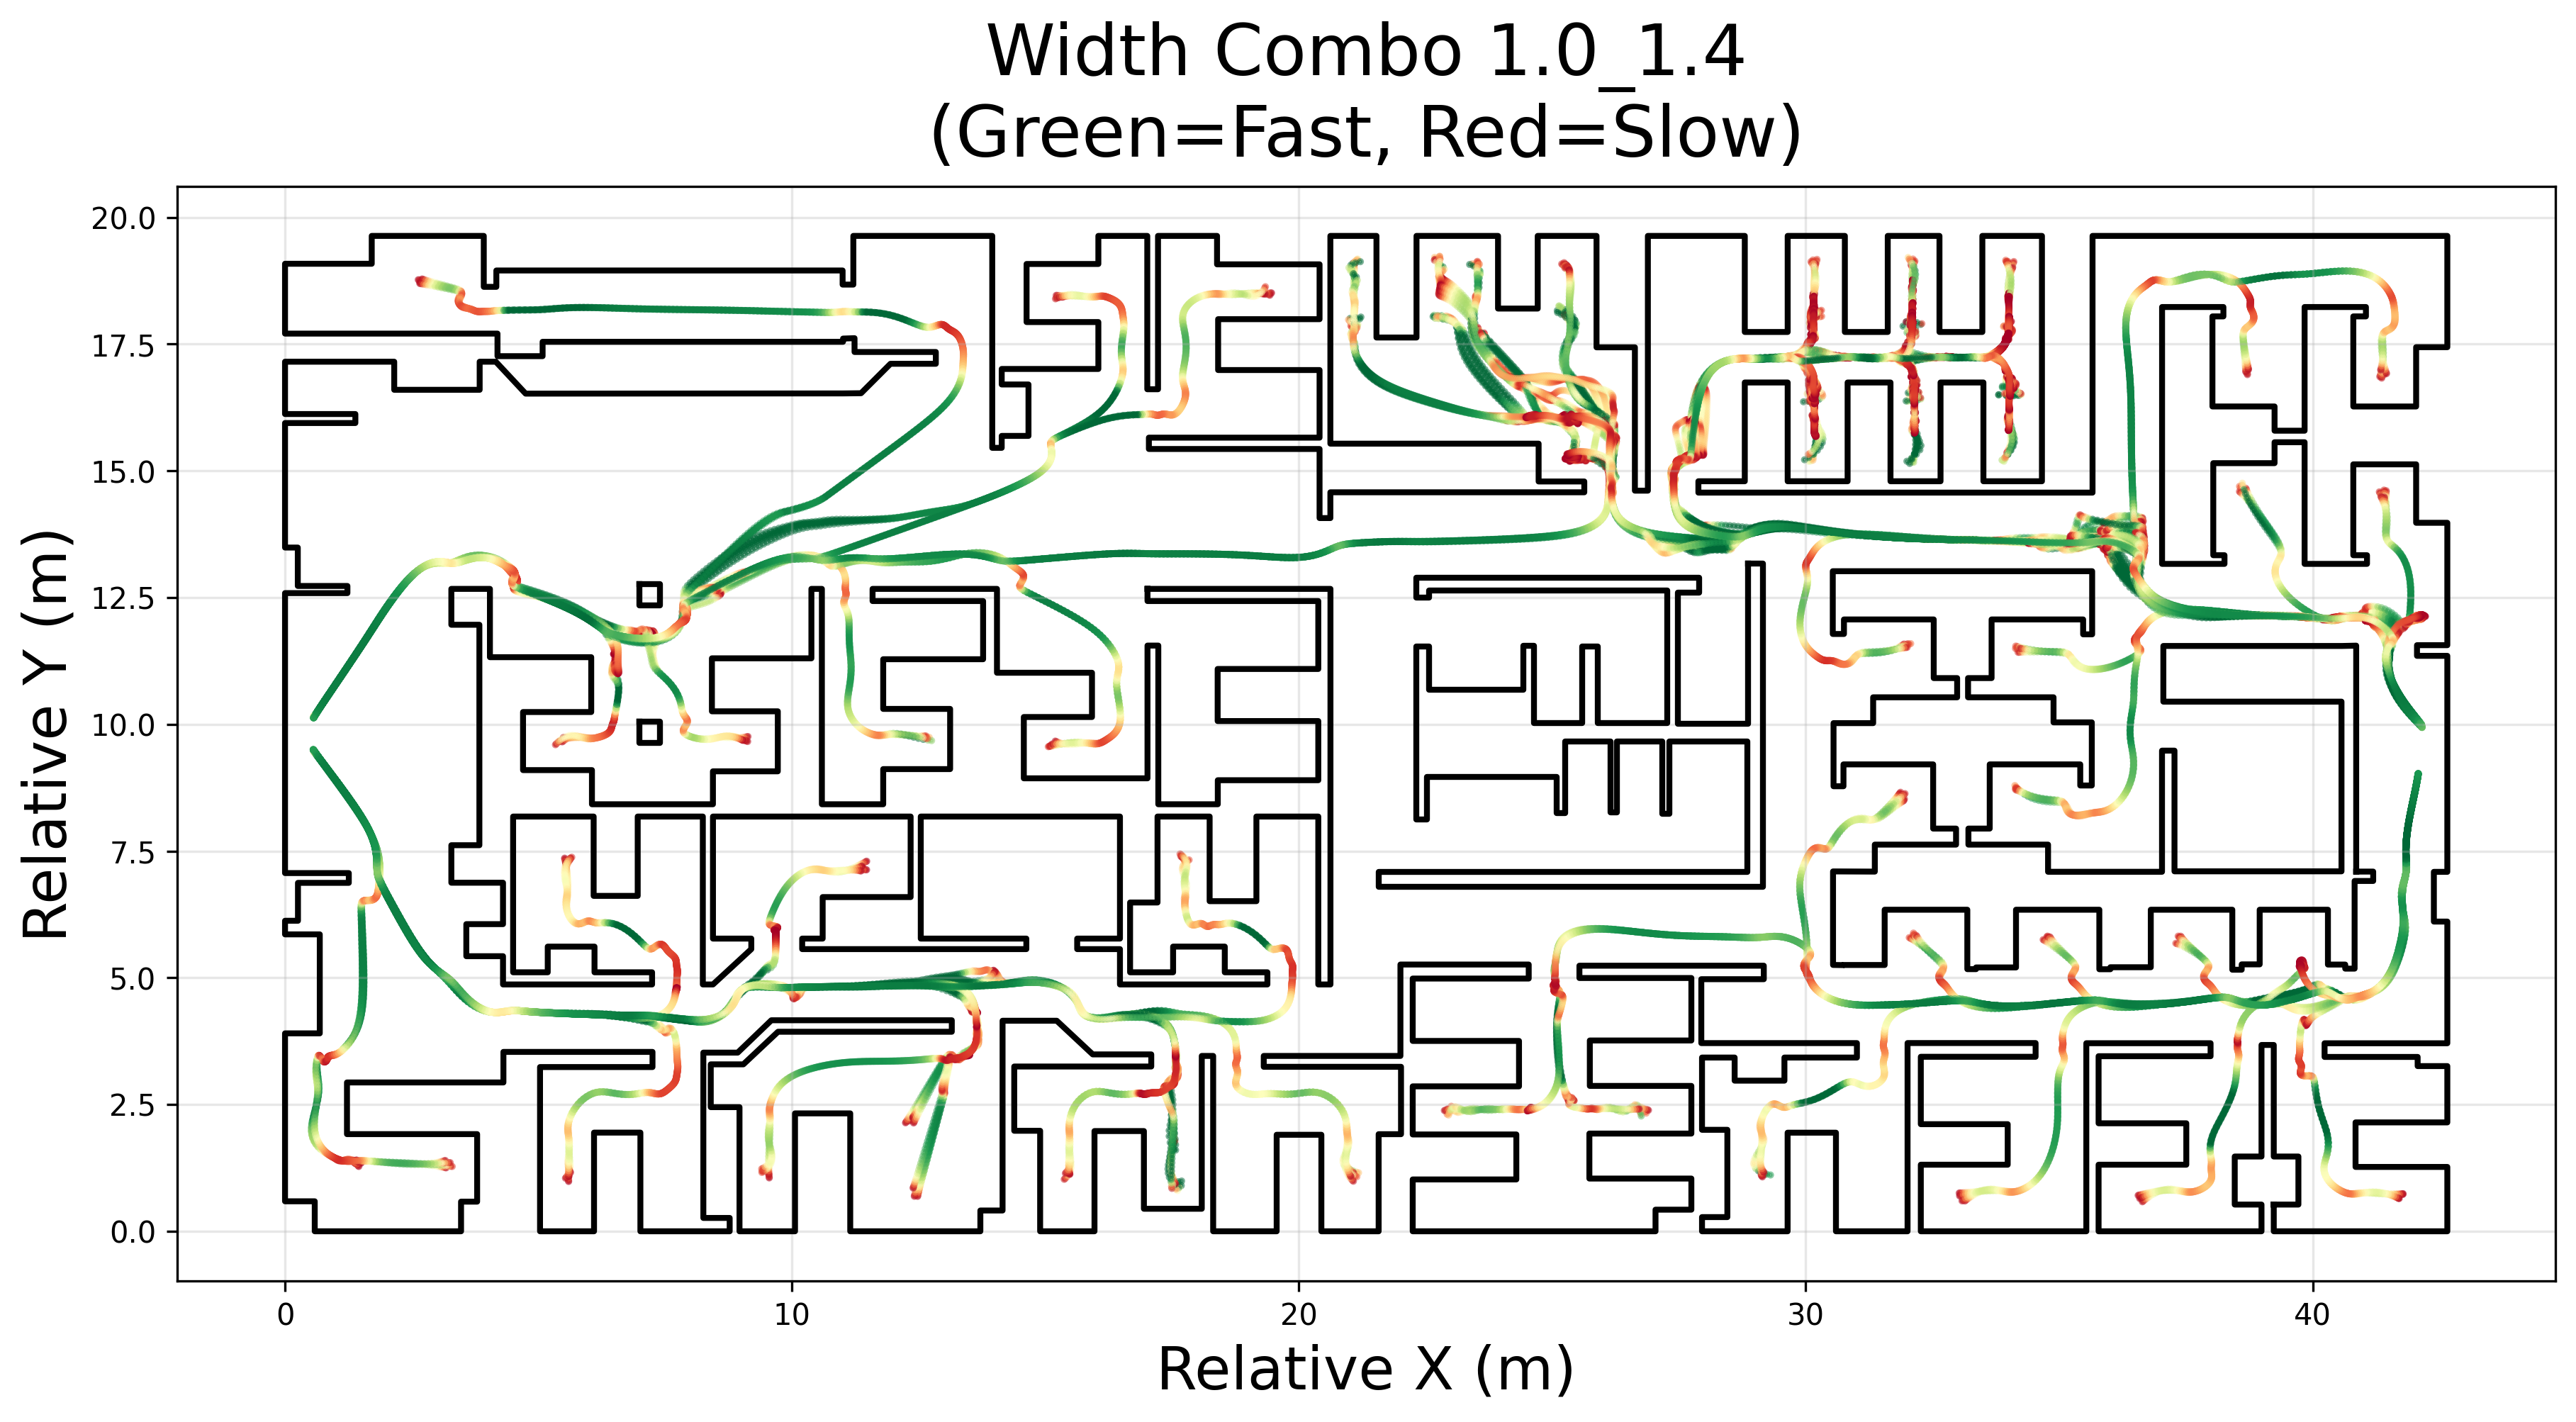
\includegraphics[width=\linewidth]{
            speed_trajectory_MultiRoom_width_1.0_1.4.png}
        \caption{Width Combo 1.0m and 1.4m}
        \label{fig:width_combo_1.0_1.4m}
    \end{subfigure}
    \begin{subfigure}[b]{.45\linewidth}
        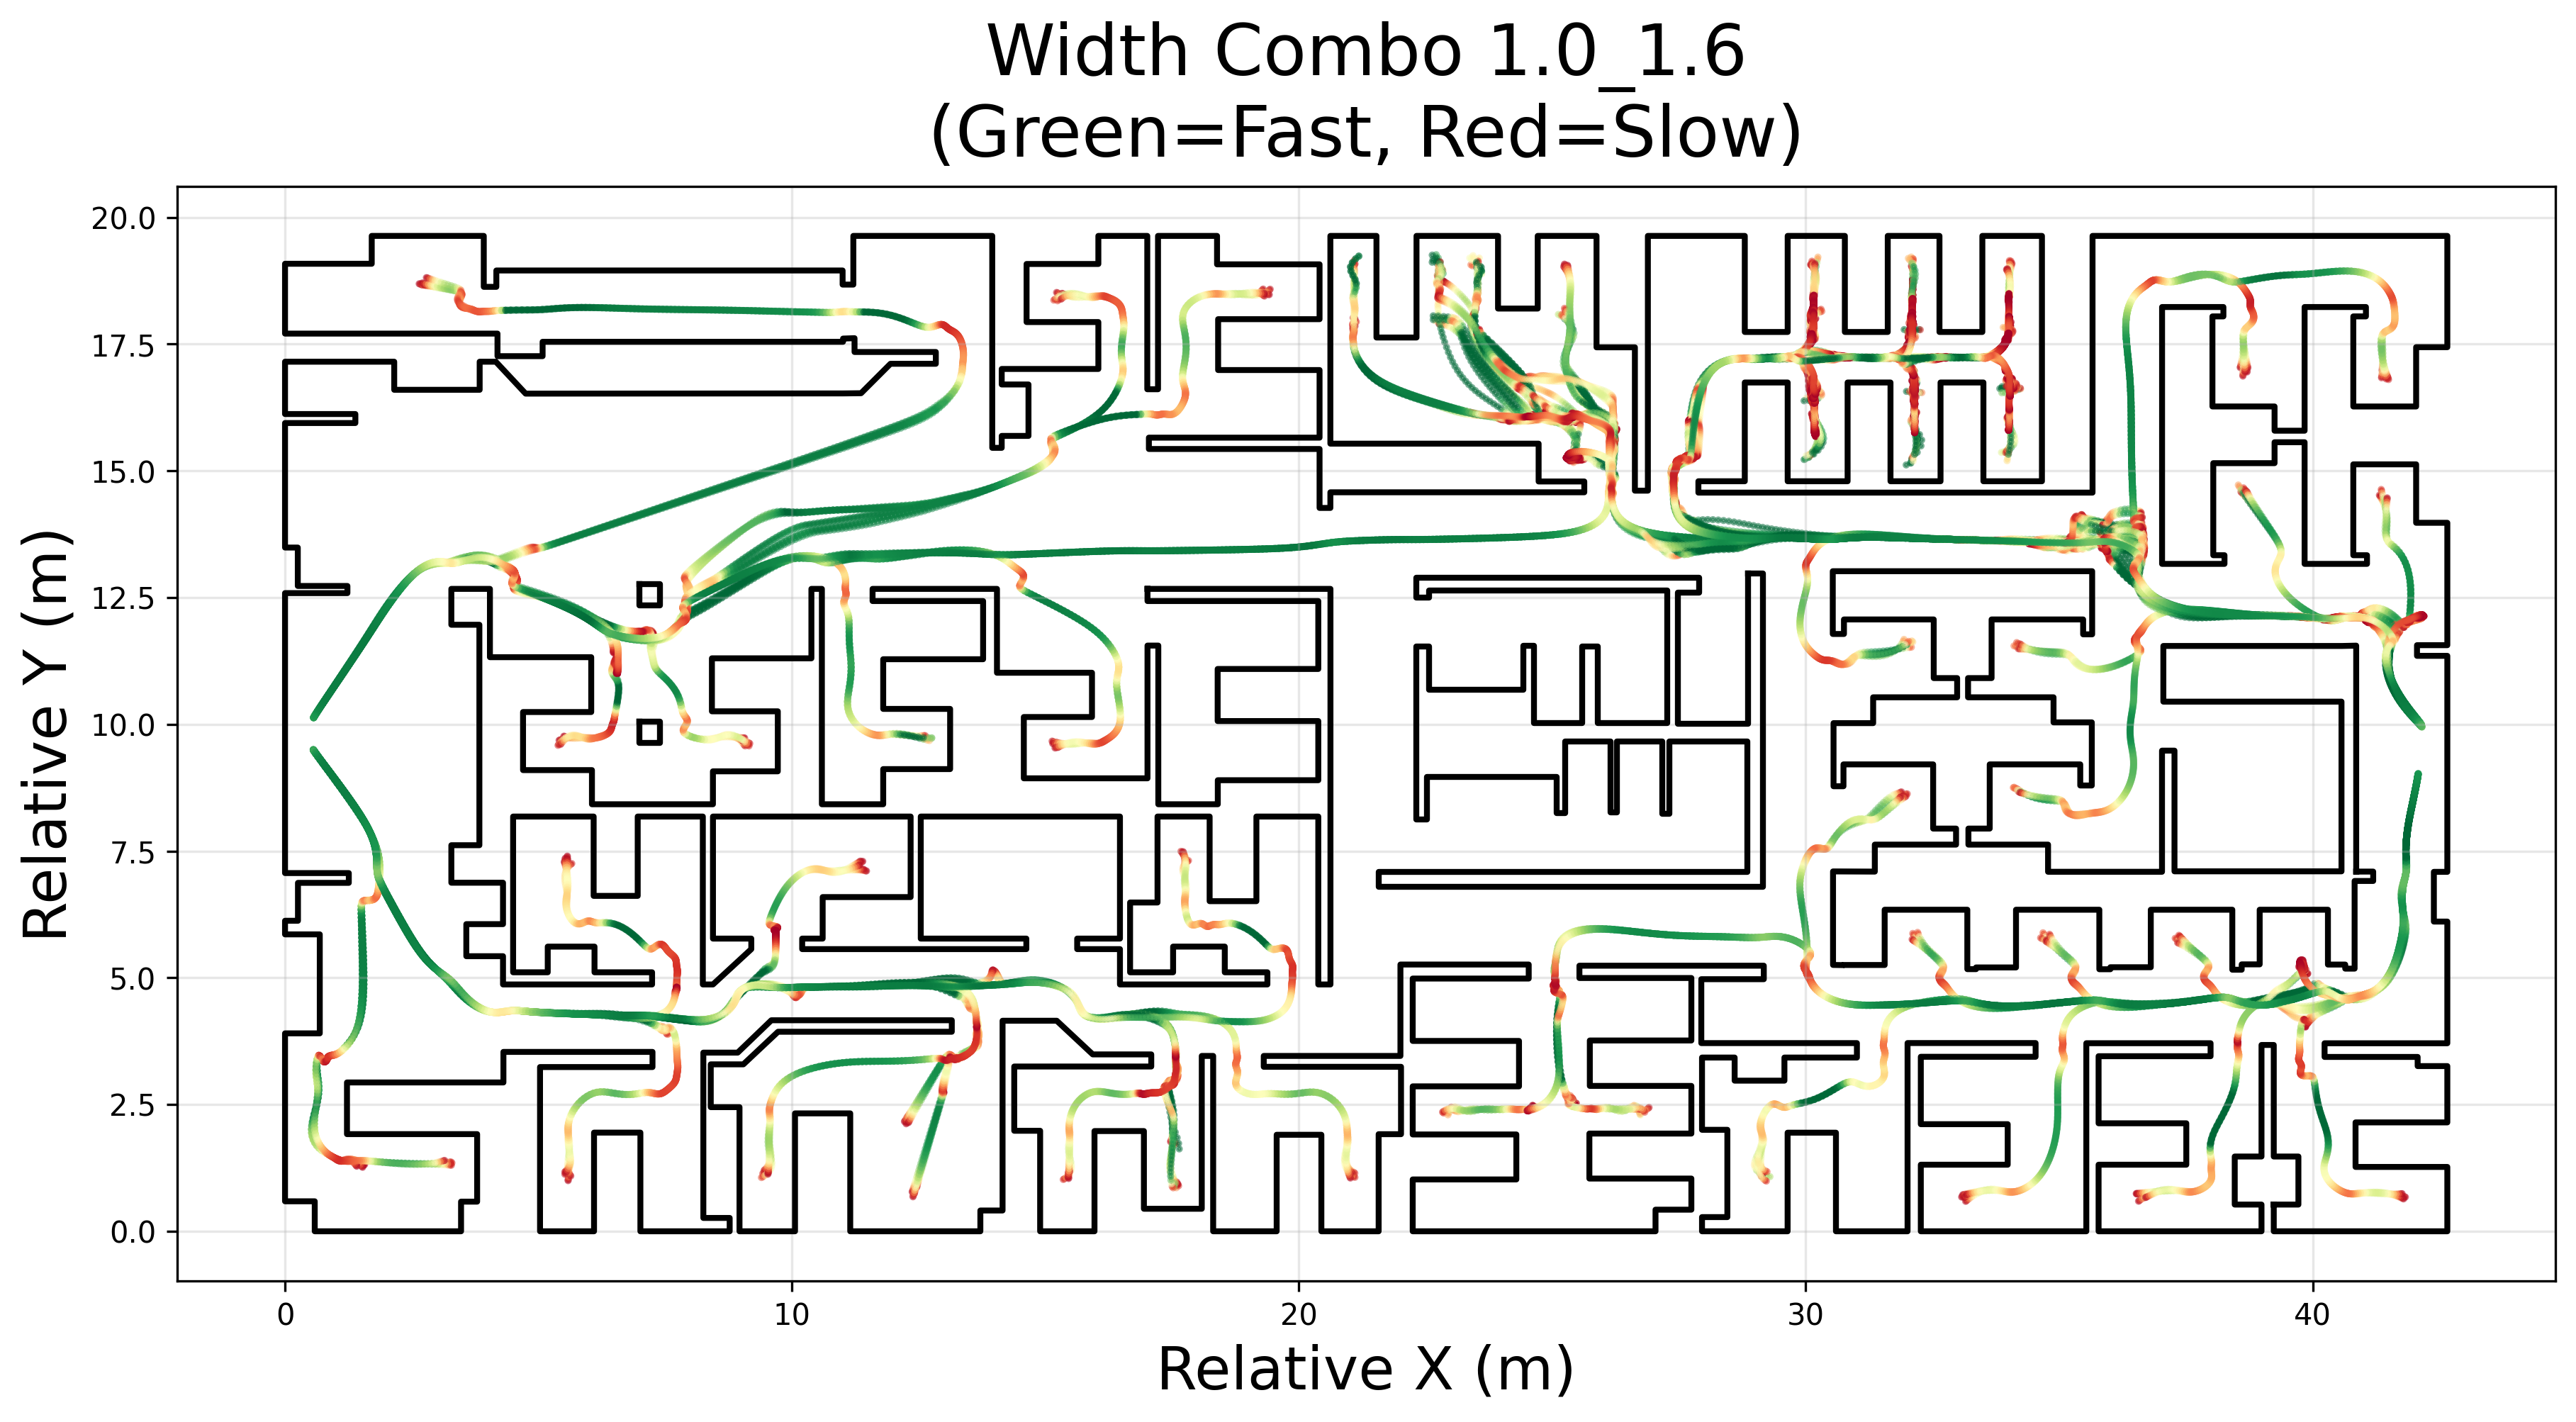
\includegraphics[width=\linewidth]{
            speed_trajectory_MultiRoom_width_1.0_1.6.png}
        \caption{Width Combo 1.0m and 1.6m}
        \label{fig:width_combo_1.0_1.6m}
    \end{subfigure}

    \caption{Speed and Trajectories for Room Door Width 1.0m}
    \label{fig:width_combo_1.0_x}
\end{figure}

According to Figure \ref{fig:width_combo_1.2_x}, keep the room door width as 1.2 m, if the corridor gate width is only 1.0 m, a large low-speed zone will appear before the merging points, with queues continuously backtracking upstream. Because the downstream release capacity is restricted by the gate width, agents can exit smoothly through the room doors, but are forced to stagnate before the narrow corridor gates, which causes longer evacuation time. As it comes to 1.2m, the low-speed zone is compressed near the gate, and the green zone in the main corridor become longer, significantly reducing the TET. When the corridor gate width reaches 1.4m, the downstream release capacity essentially matches the supply from upstream, backtracking almost disappears and only several low-speed points occur at some corners, therefore the evacuation time drops to its lowest and variation among the runs converges. Even when the corridor gate width is widened to 1.6m, the agents flow pattern is almost the same as that at 1.4m, because the real limitation is the 1.2m room door width, so the TET will not decrease more. However, since congestion becomes more difficult to form, results are more stable and the standard deviation will decrease further. To summerize, when the room door width is 1.2 m, simply increasing the corridor door from 1.0 m to 1.4 m can basicly eliminate queuing, allow the mean TET to drop rapidly and help the system to become stable, while continued widening would not benefit more in stability.

\begin{figure}[h]
    \centering
    \begin{subfigure}[b]{.45\linewidth}
        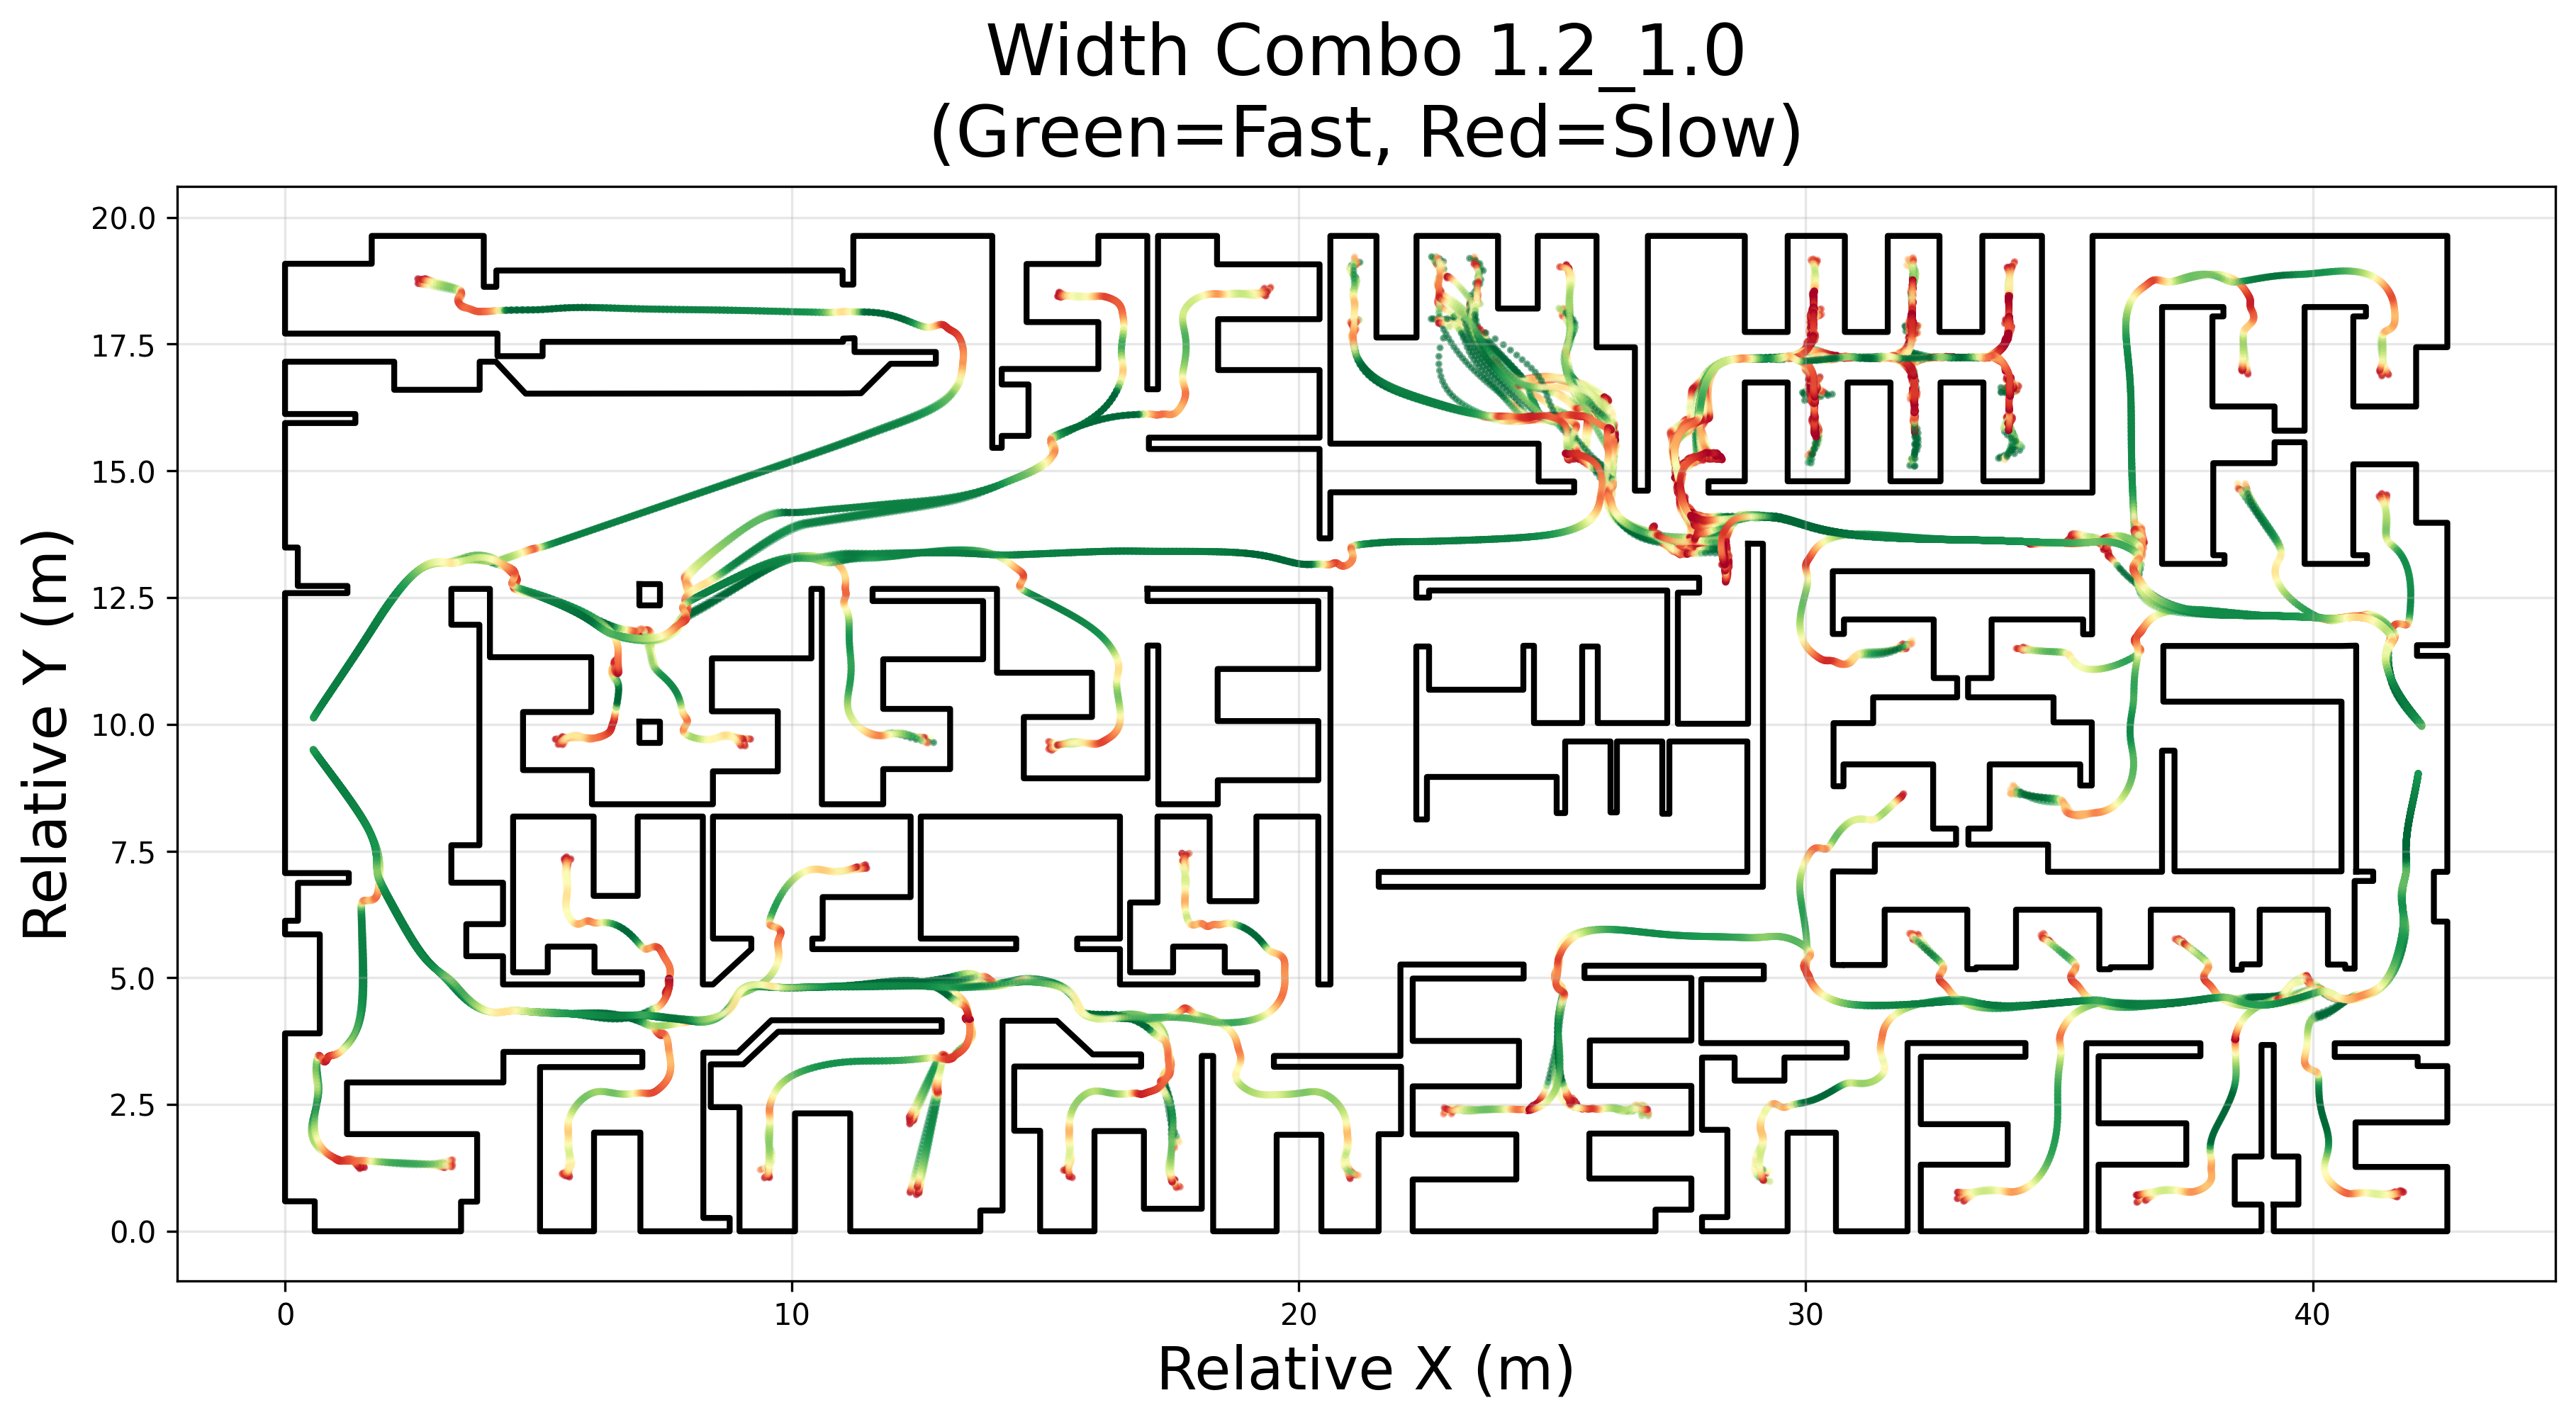
\includegraphics[width=\linewidth]{
            speed_trajectory_MultiRoom_width_1.2_1.0.png}
        \caption{Width Combo 1.2m and 1.0m}
        \label{fig:width_combo_1.2_1.0m}
    \end{subfigure}
    \begin{subfigure}[b]{.45\linewidth}
        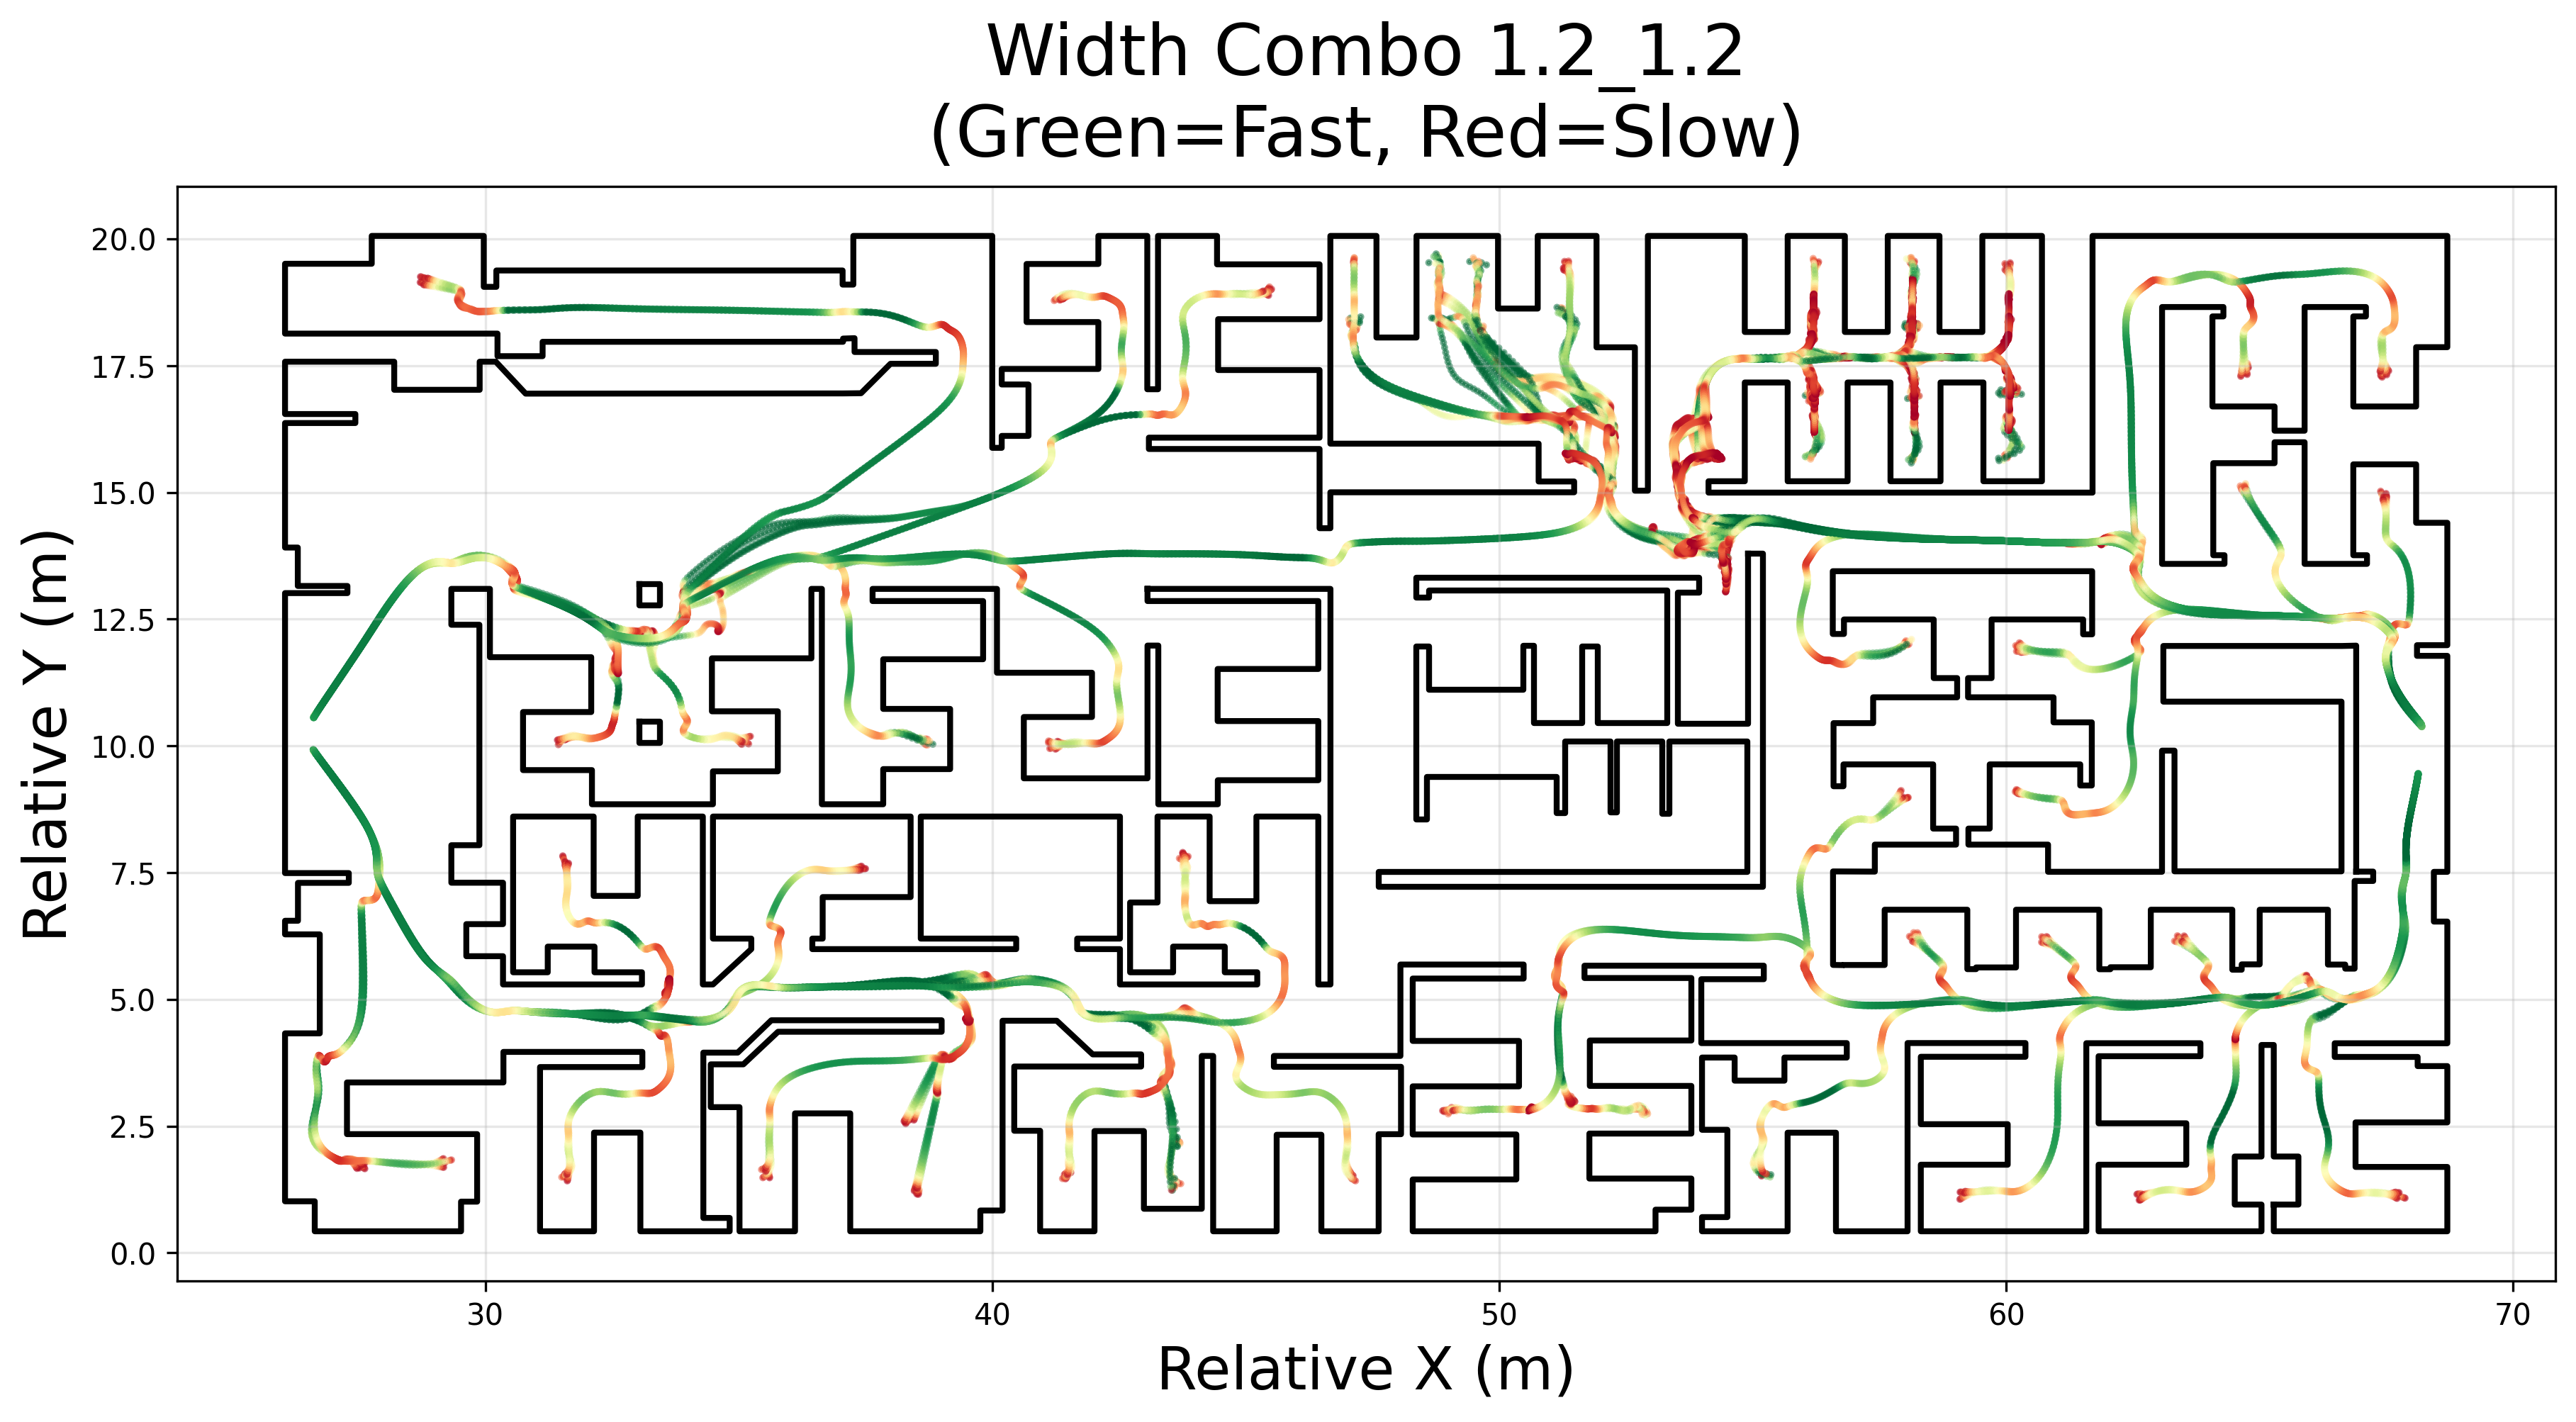
\includegraphics[width=\linewidth]{
            speed_trajectory_MultiRoom_width_1.2_1.2.png}
        \caption{Width Combo 1.2m and 1.2m}
        \label{fig:width_combo_1.2_1.2m}
    \end{subfigure}

    \begin{subfigure}[b]{.45\linewidth}
        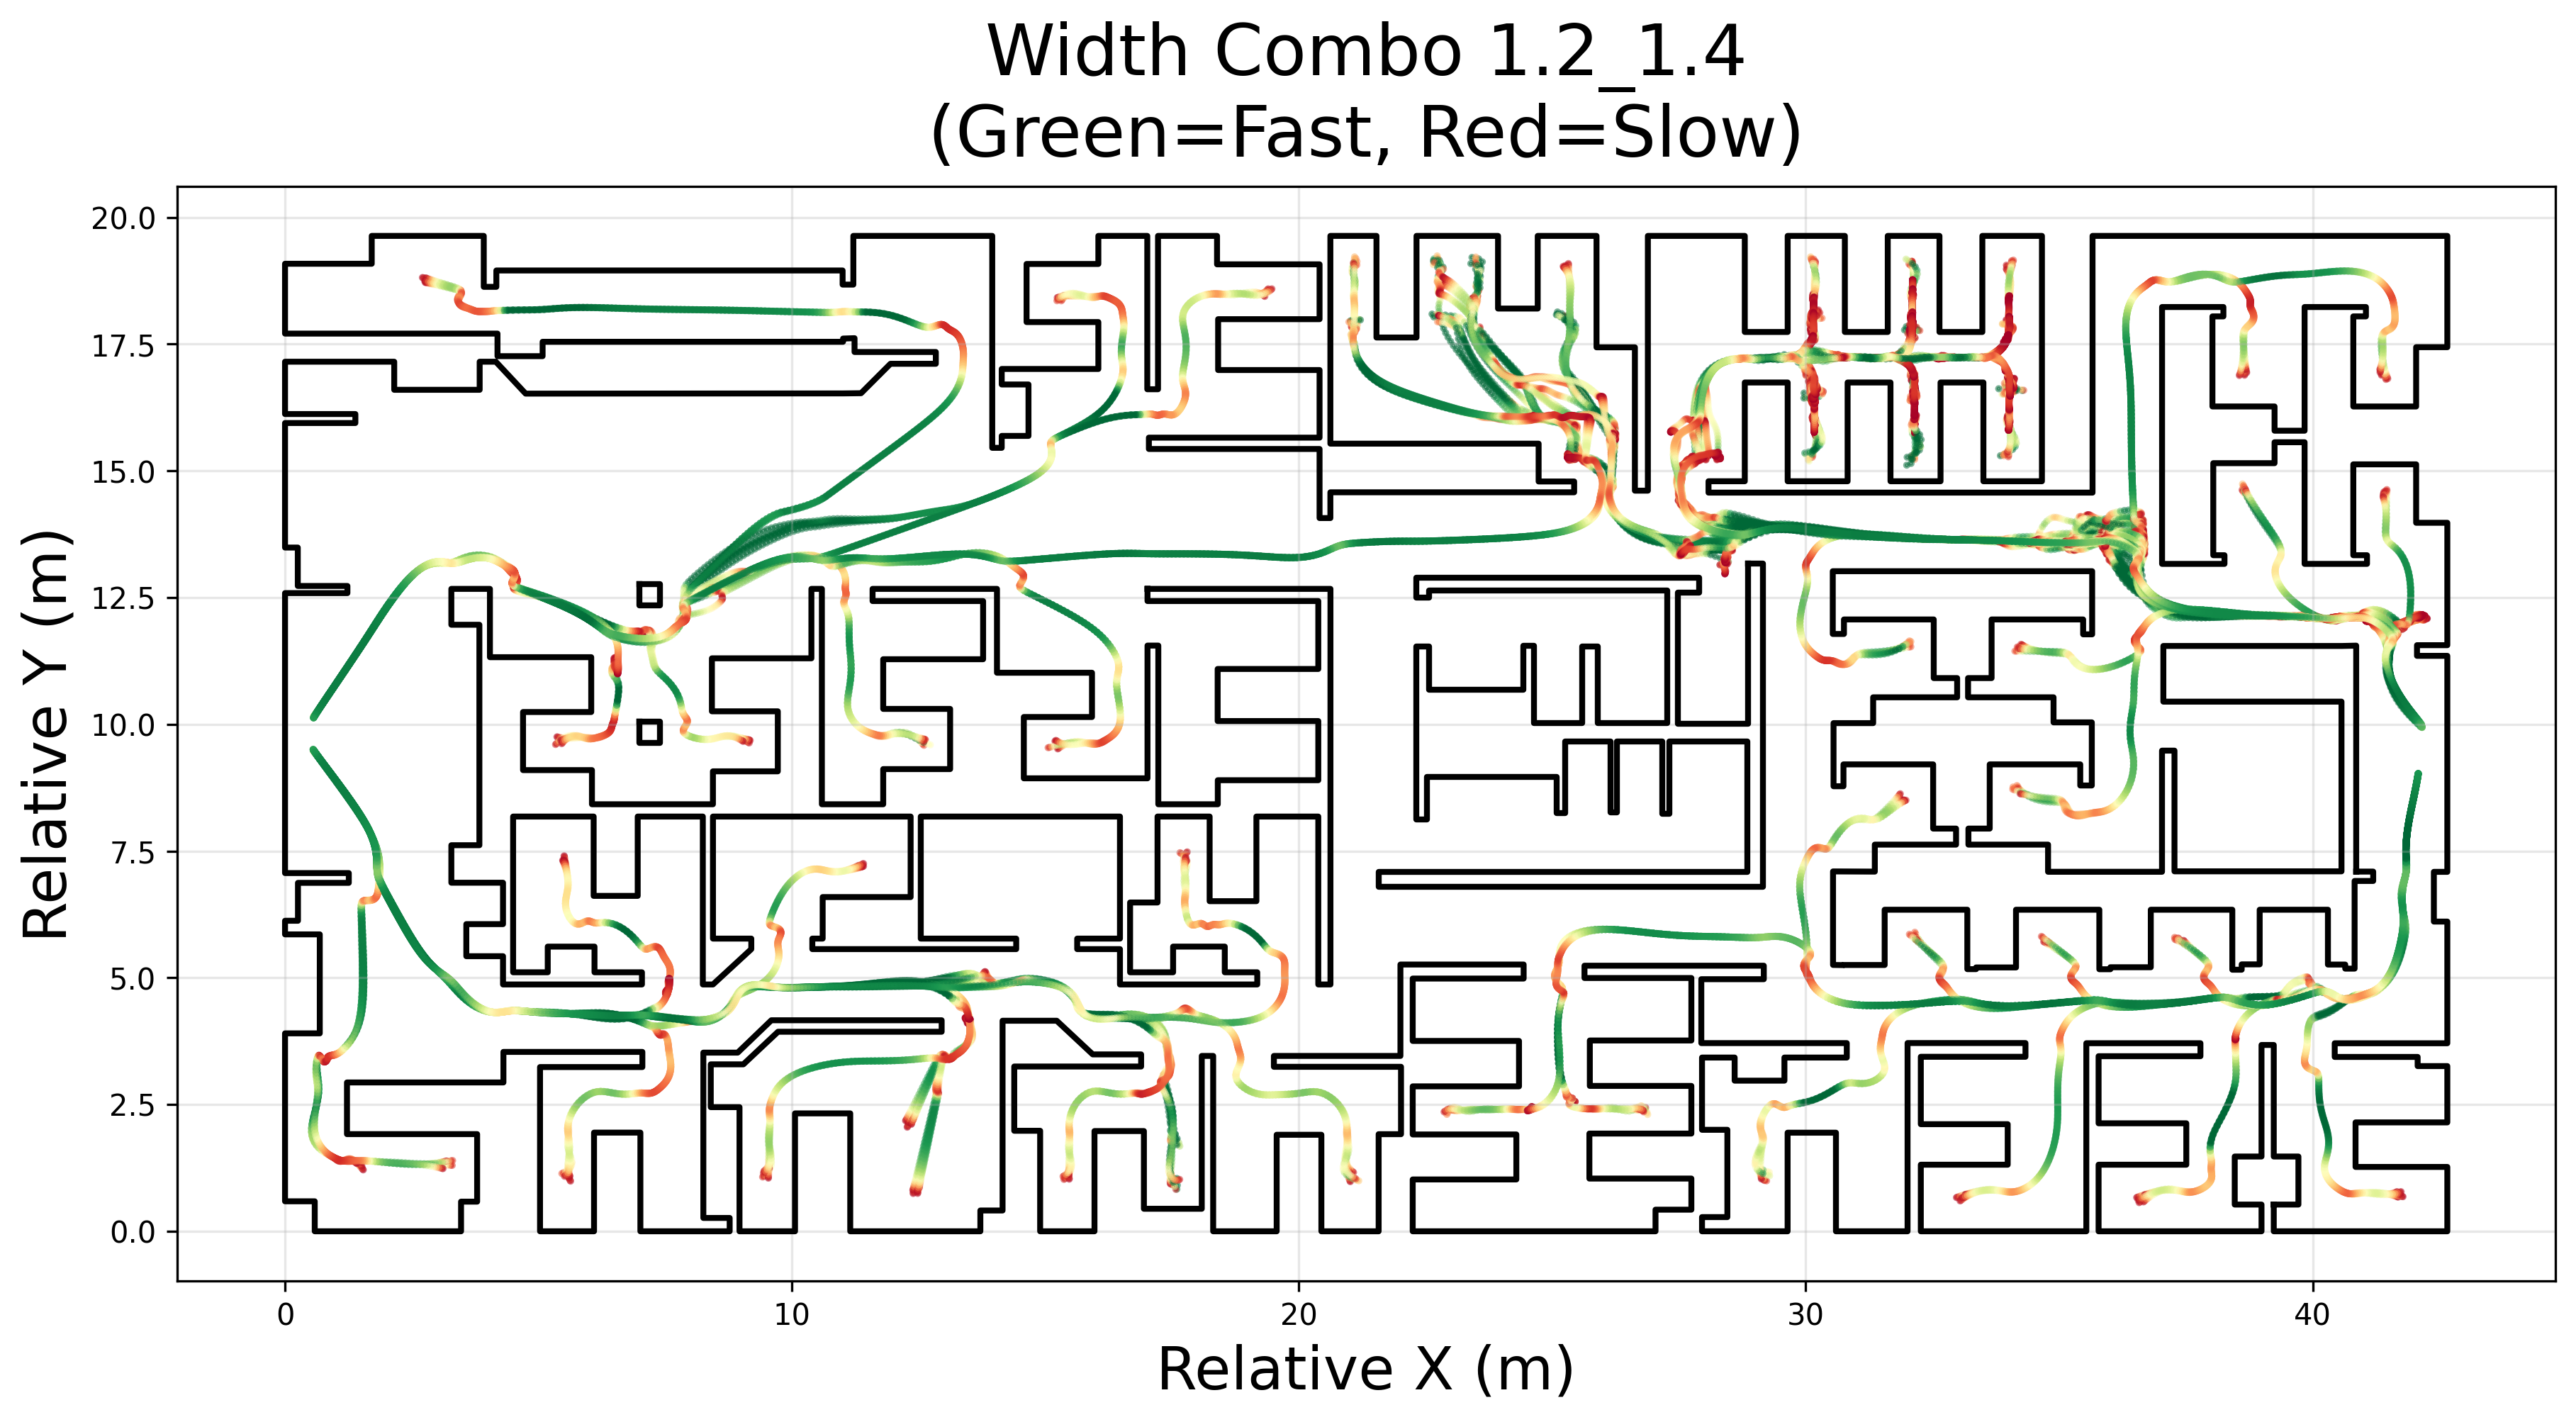
\includegraphics[width=\linewidth]{
            speed_trajectory_MultiRoom_width_1.2_1.4.png}
        \caption{Width Combo 1.2m and 1.4m}
        \label{fig:width_combo_1.2_1.4m}
    \end{subfigure}
    \begin{subfigure}[b]{.45\linewidth}
        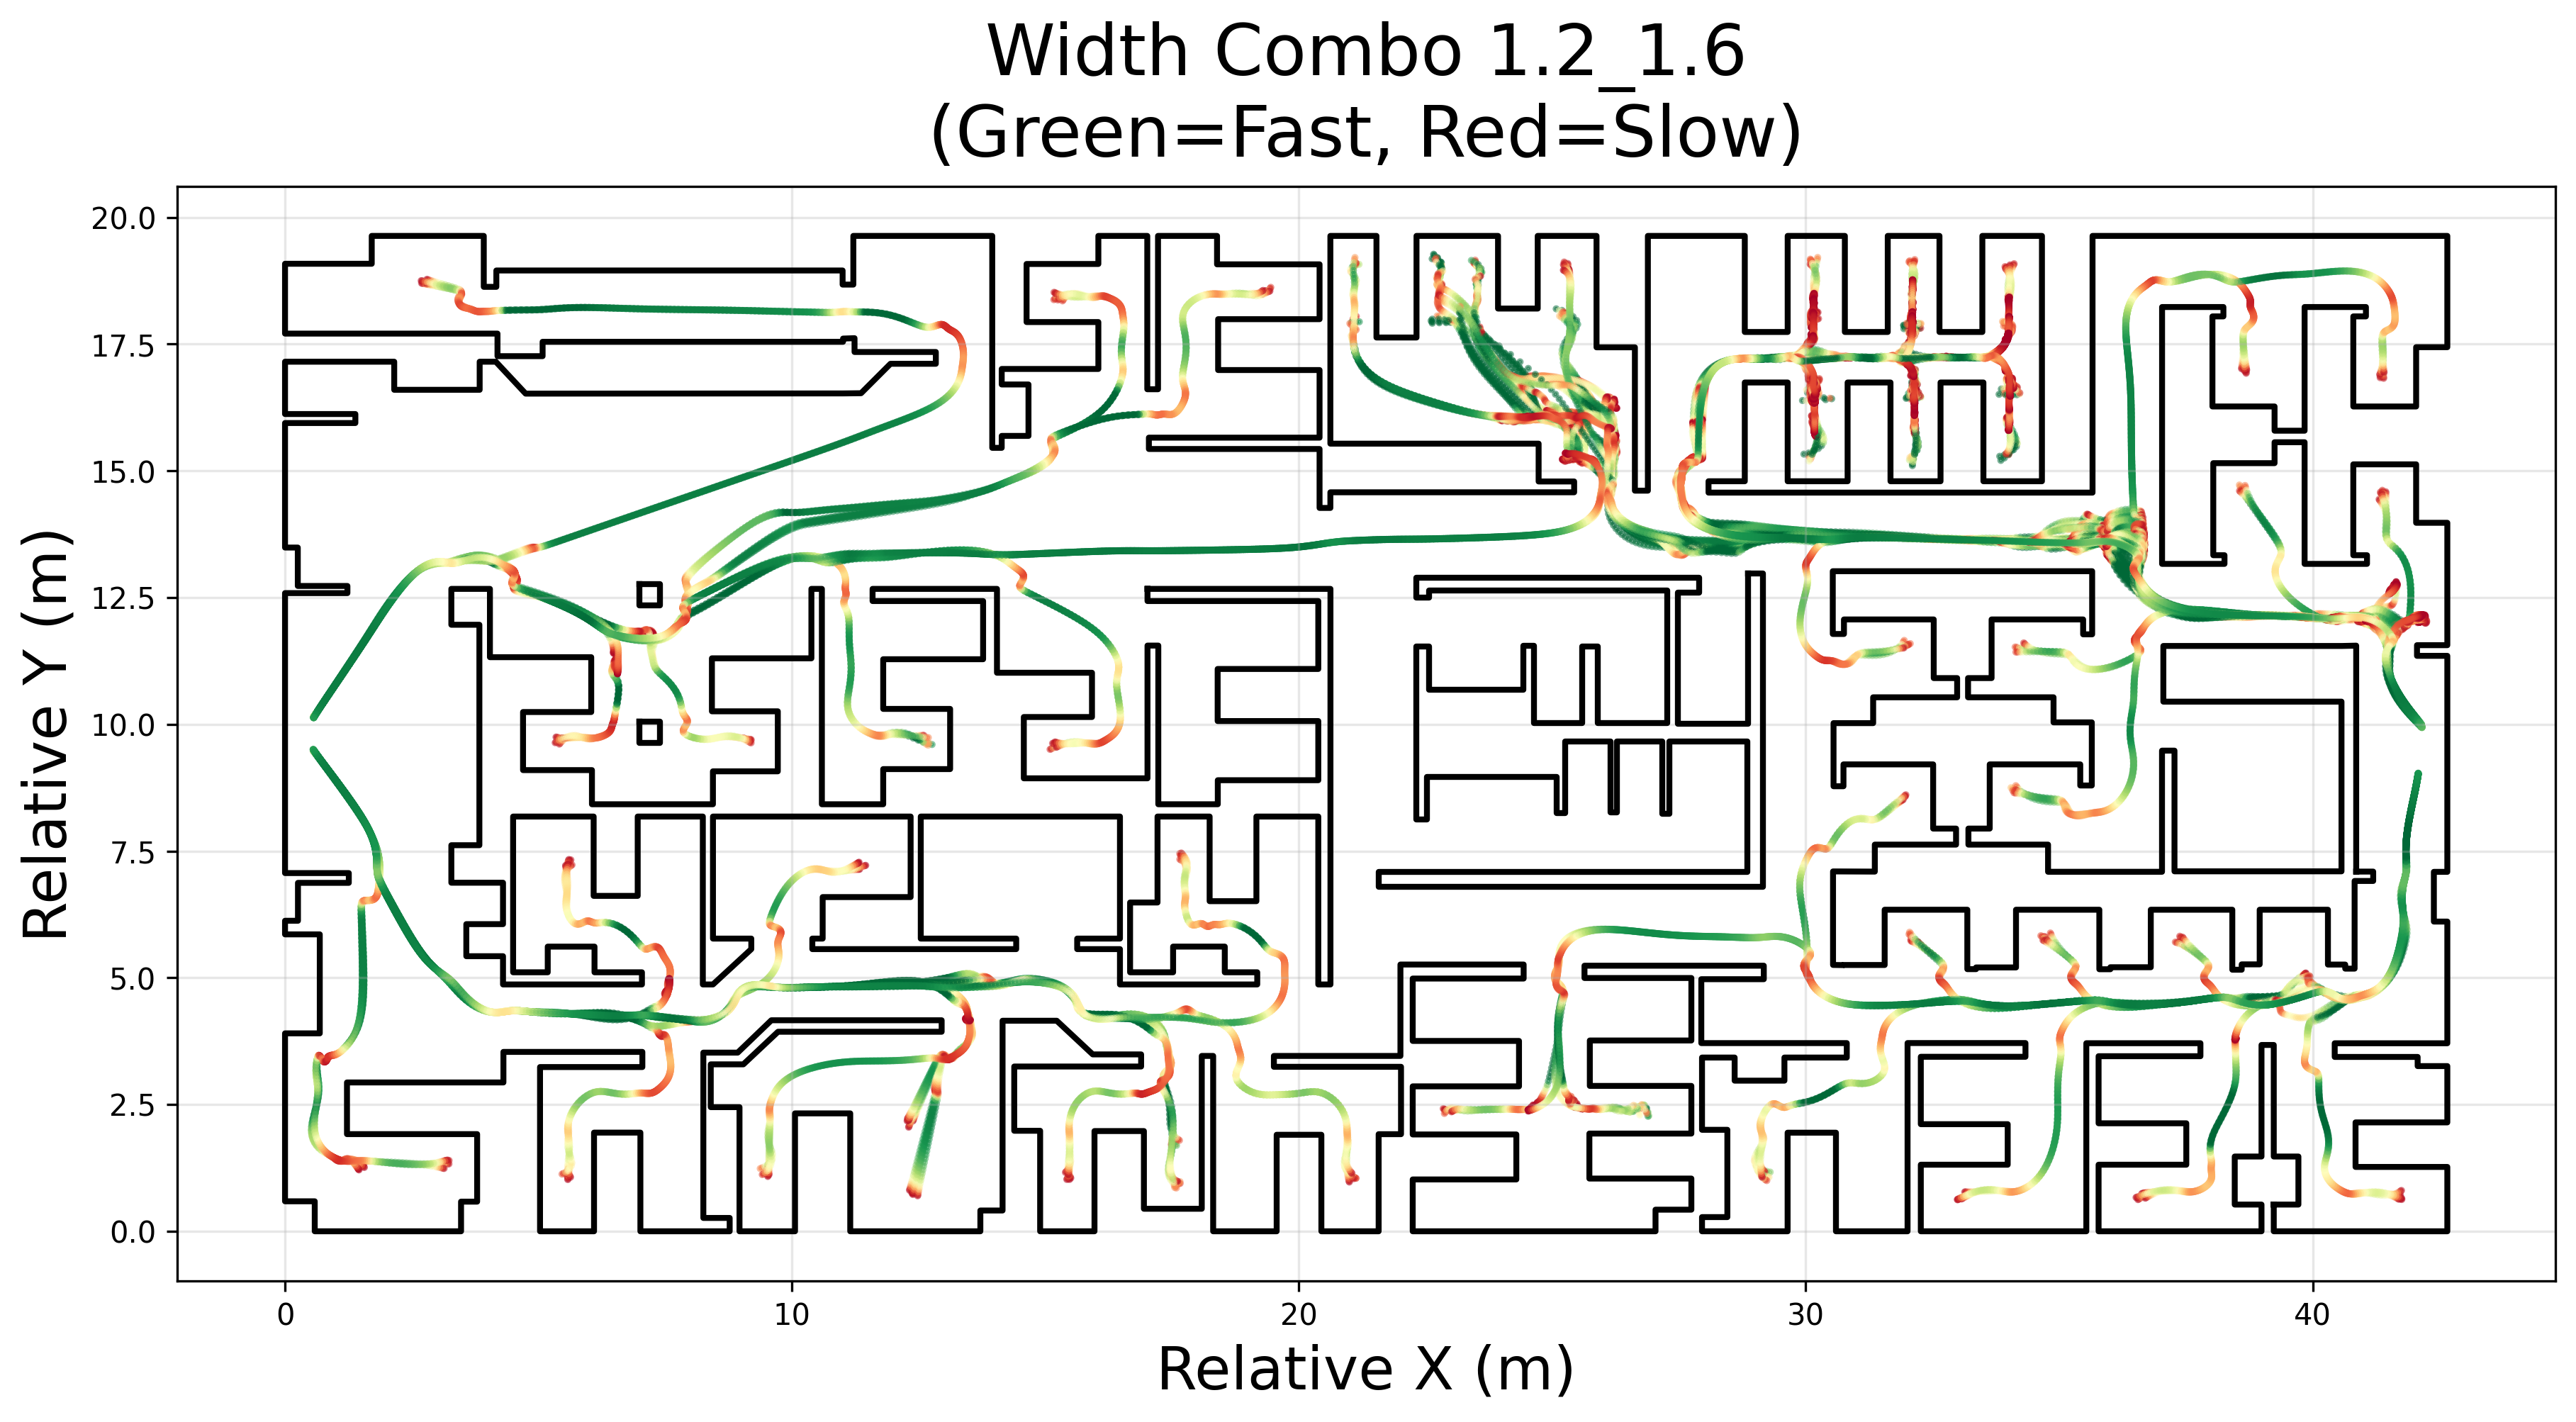
\includegraphics[width=\linewidth]{
            speed_trajectory_MultiRoom_width_1.2_1.6.png}
        \caption{Width Combo 1.2m and 1.6m}
        \label{fig:width_combo_1.2_1.6m}
    \end{subfigure}

    \caption{Speed and Trajectories for Room Door Width 1.2m}
    \label{fig:width_combo_1.2_x}
\end{figure}

When the room door width is fixed at 1.4m \ref{fig:width_combo_1.4_x}, compared to 1.2 m \ref{fig:width_combo_1.2_x}, both configurations share common characteristics when the corridor gate is only 1.0m: upstream supply significantly exceeds downstream discharge capacity, both form large low-velocity zones before convergence accompanied by backflow/stagnation, resulting in the highest evacuation times and fluctuations with the most unstable system performance. The difference is that the 1.4 m configuration has stronger upstream supply, thus showing more pronounced response to the 1.0 m bottleneck, with higher peak TET and standard deviation. As the corridor gate increases to 1.2 m, both configurations show compressed low-velocity zones, longer continuous green sections in the main pathway, reduced backflow, decreased average times and converging fluctuations. However, the 1.4 m configuration maintains higher residual fluctuations than the 1.2 m configuration due to more abundant supply. When the corridor gate reaches 1.4 m, both achieve basic matching between downstream release capacity and upstream supply: trajectories become more smooth, low-speed points only briefly occur at corners, backtracking disappears, and TET enters a lower and more stable range. When the corridor gate width is further widened to 1.6 m, the flow patterns of both configurations remain nearly identical to those at 1.4 m, both limited by the room door width becoming the bottleneck. Average evacuation time show little change but stability further improves, with the 1.4 m room door configuration achieving lower standard deviation after stabilization due to its stronger baseline supply.

\begin{figure}[h]
    \centering
        \begin{subfigure}[b]{.45\linewidth}
        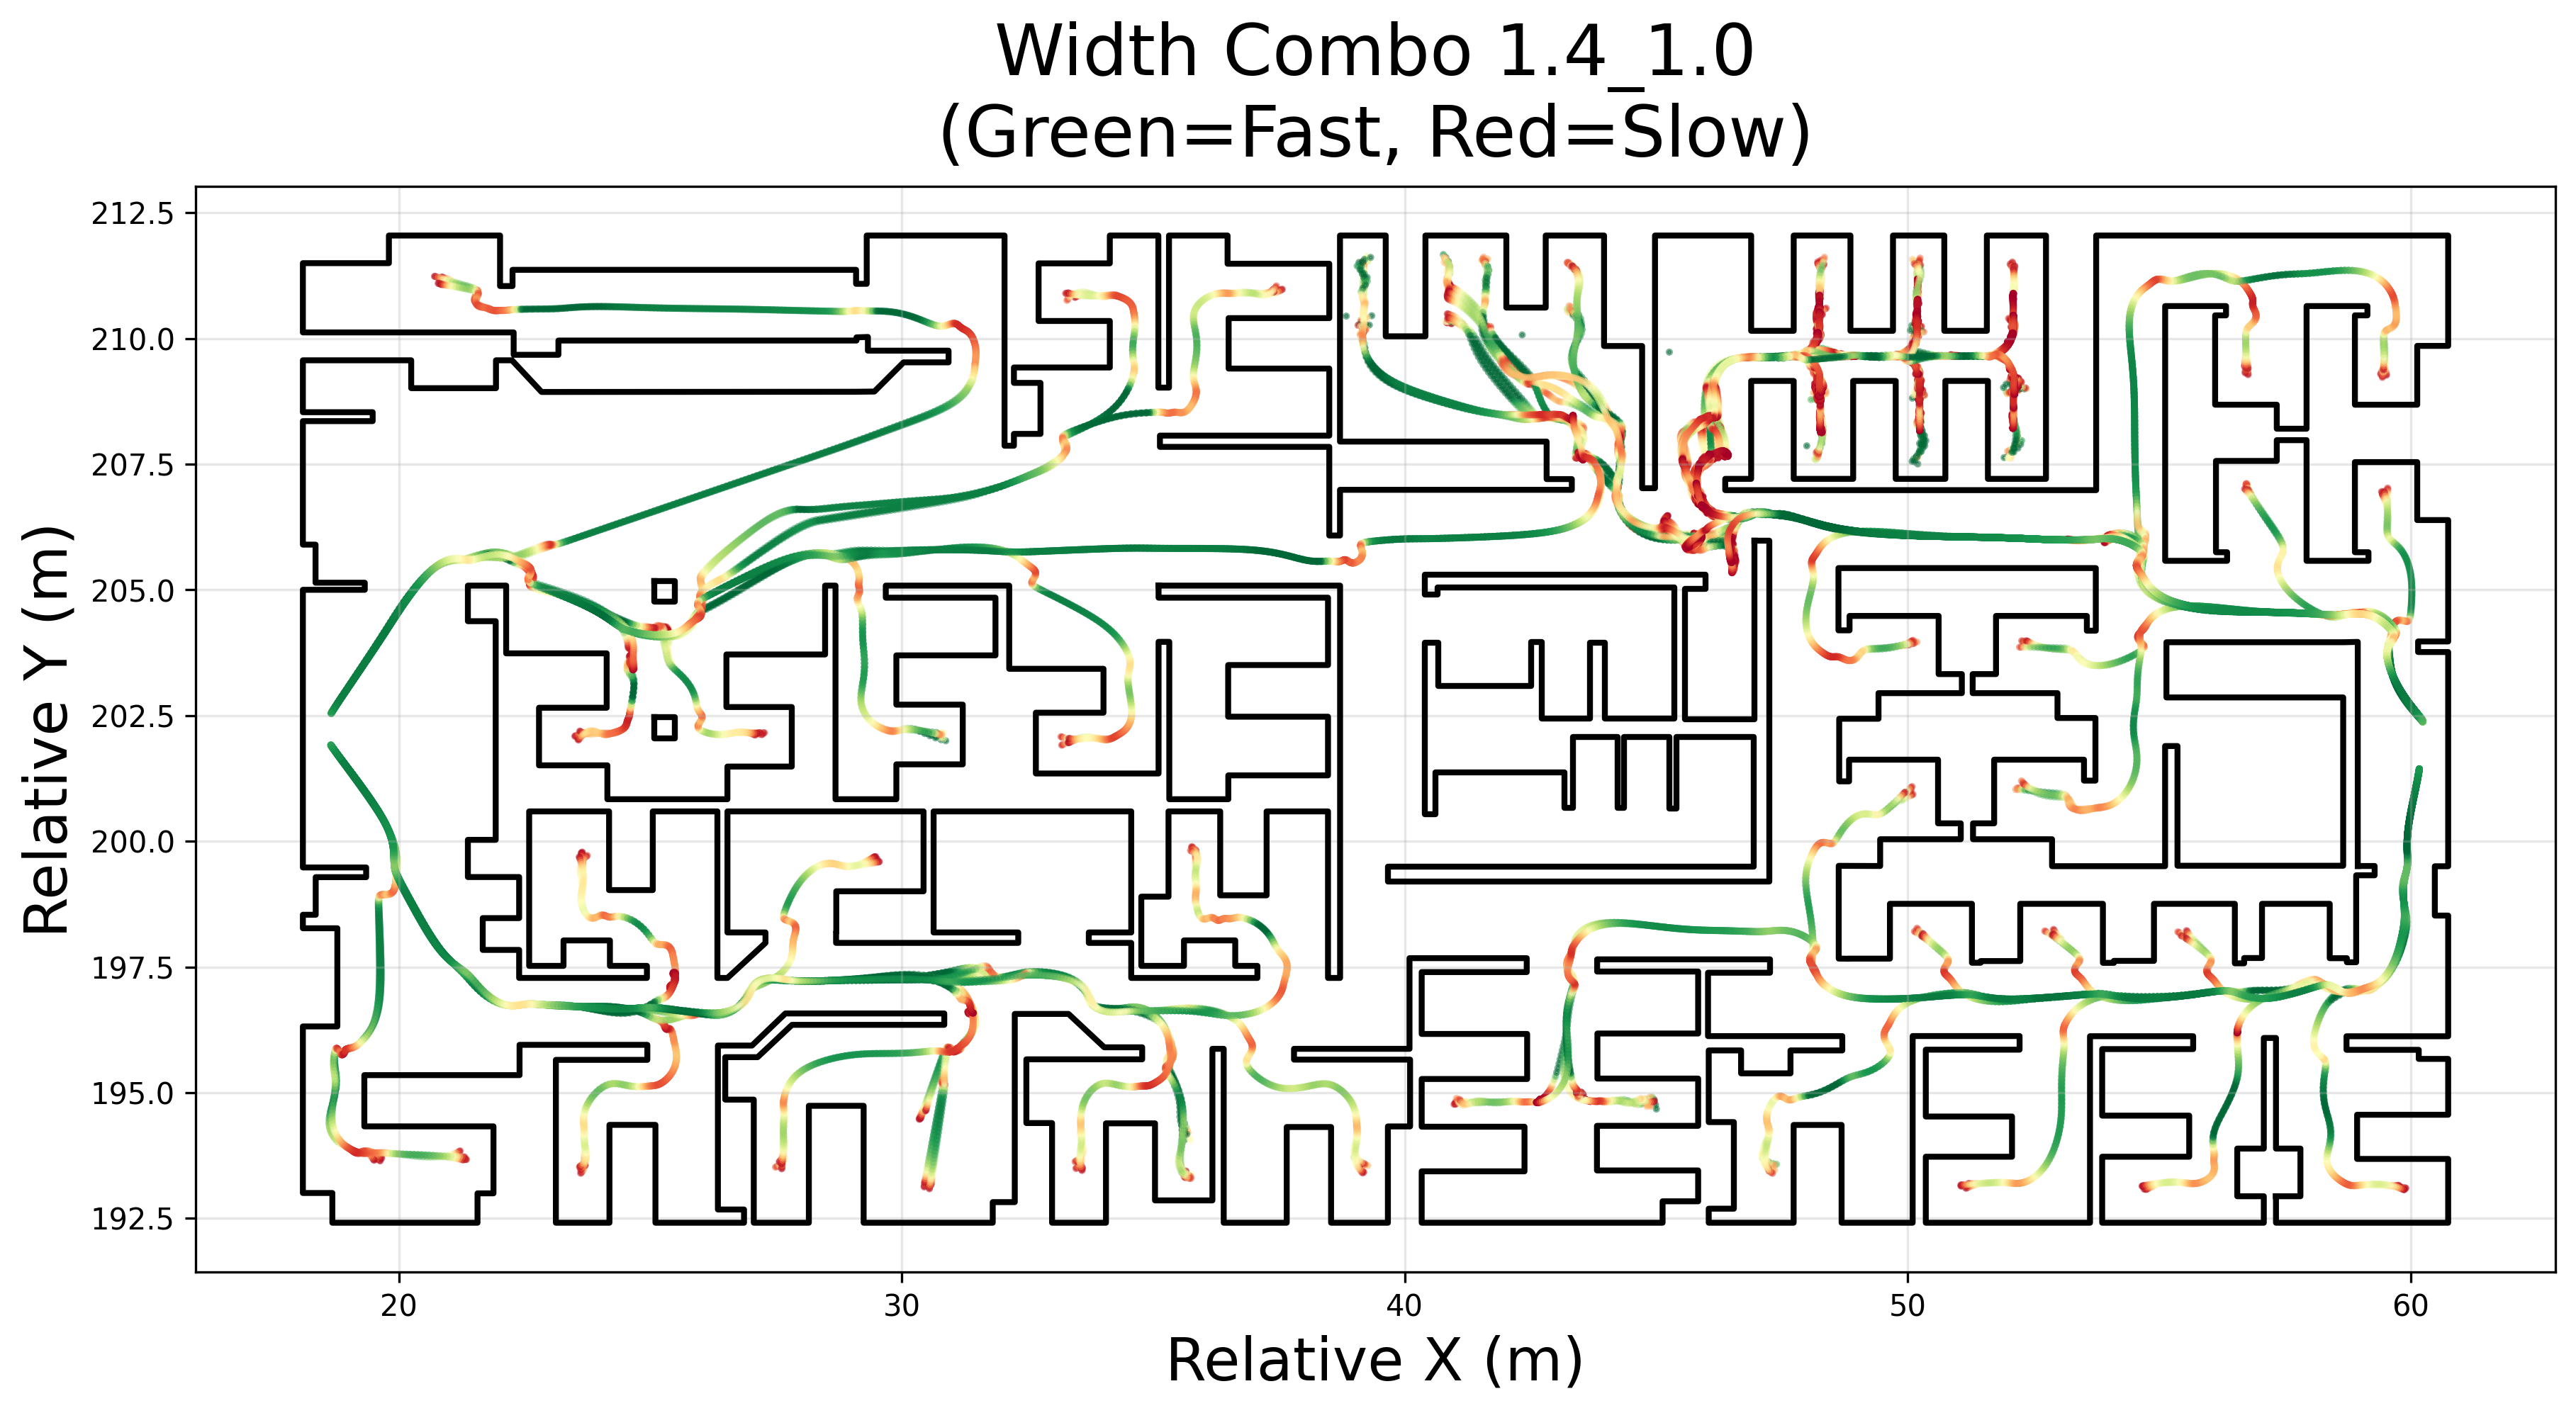
\includegraphics[width=\linewidth]{
            speed_trajectory_MultiRoom_width_1.4_1.0.png}
        \caption{Width Combo 1.4m and 1.0m}
        \label{fig:width_combo_1.4_1.0m}
    \end{subfigure}
    \begin{subfigure}[b]{.45\linewidth}
        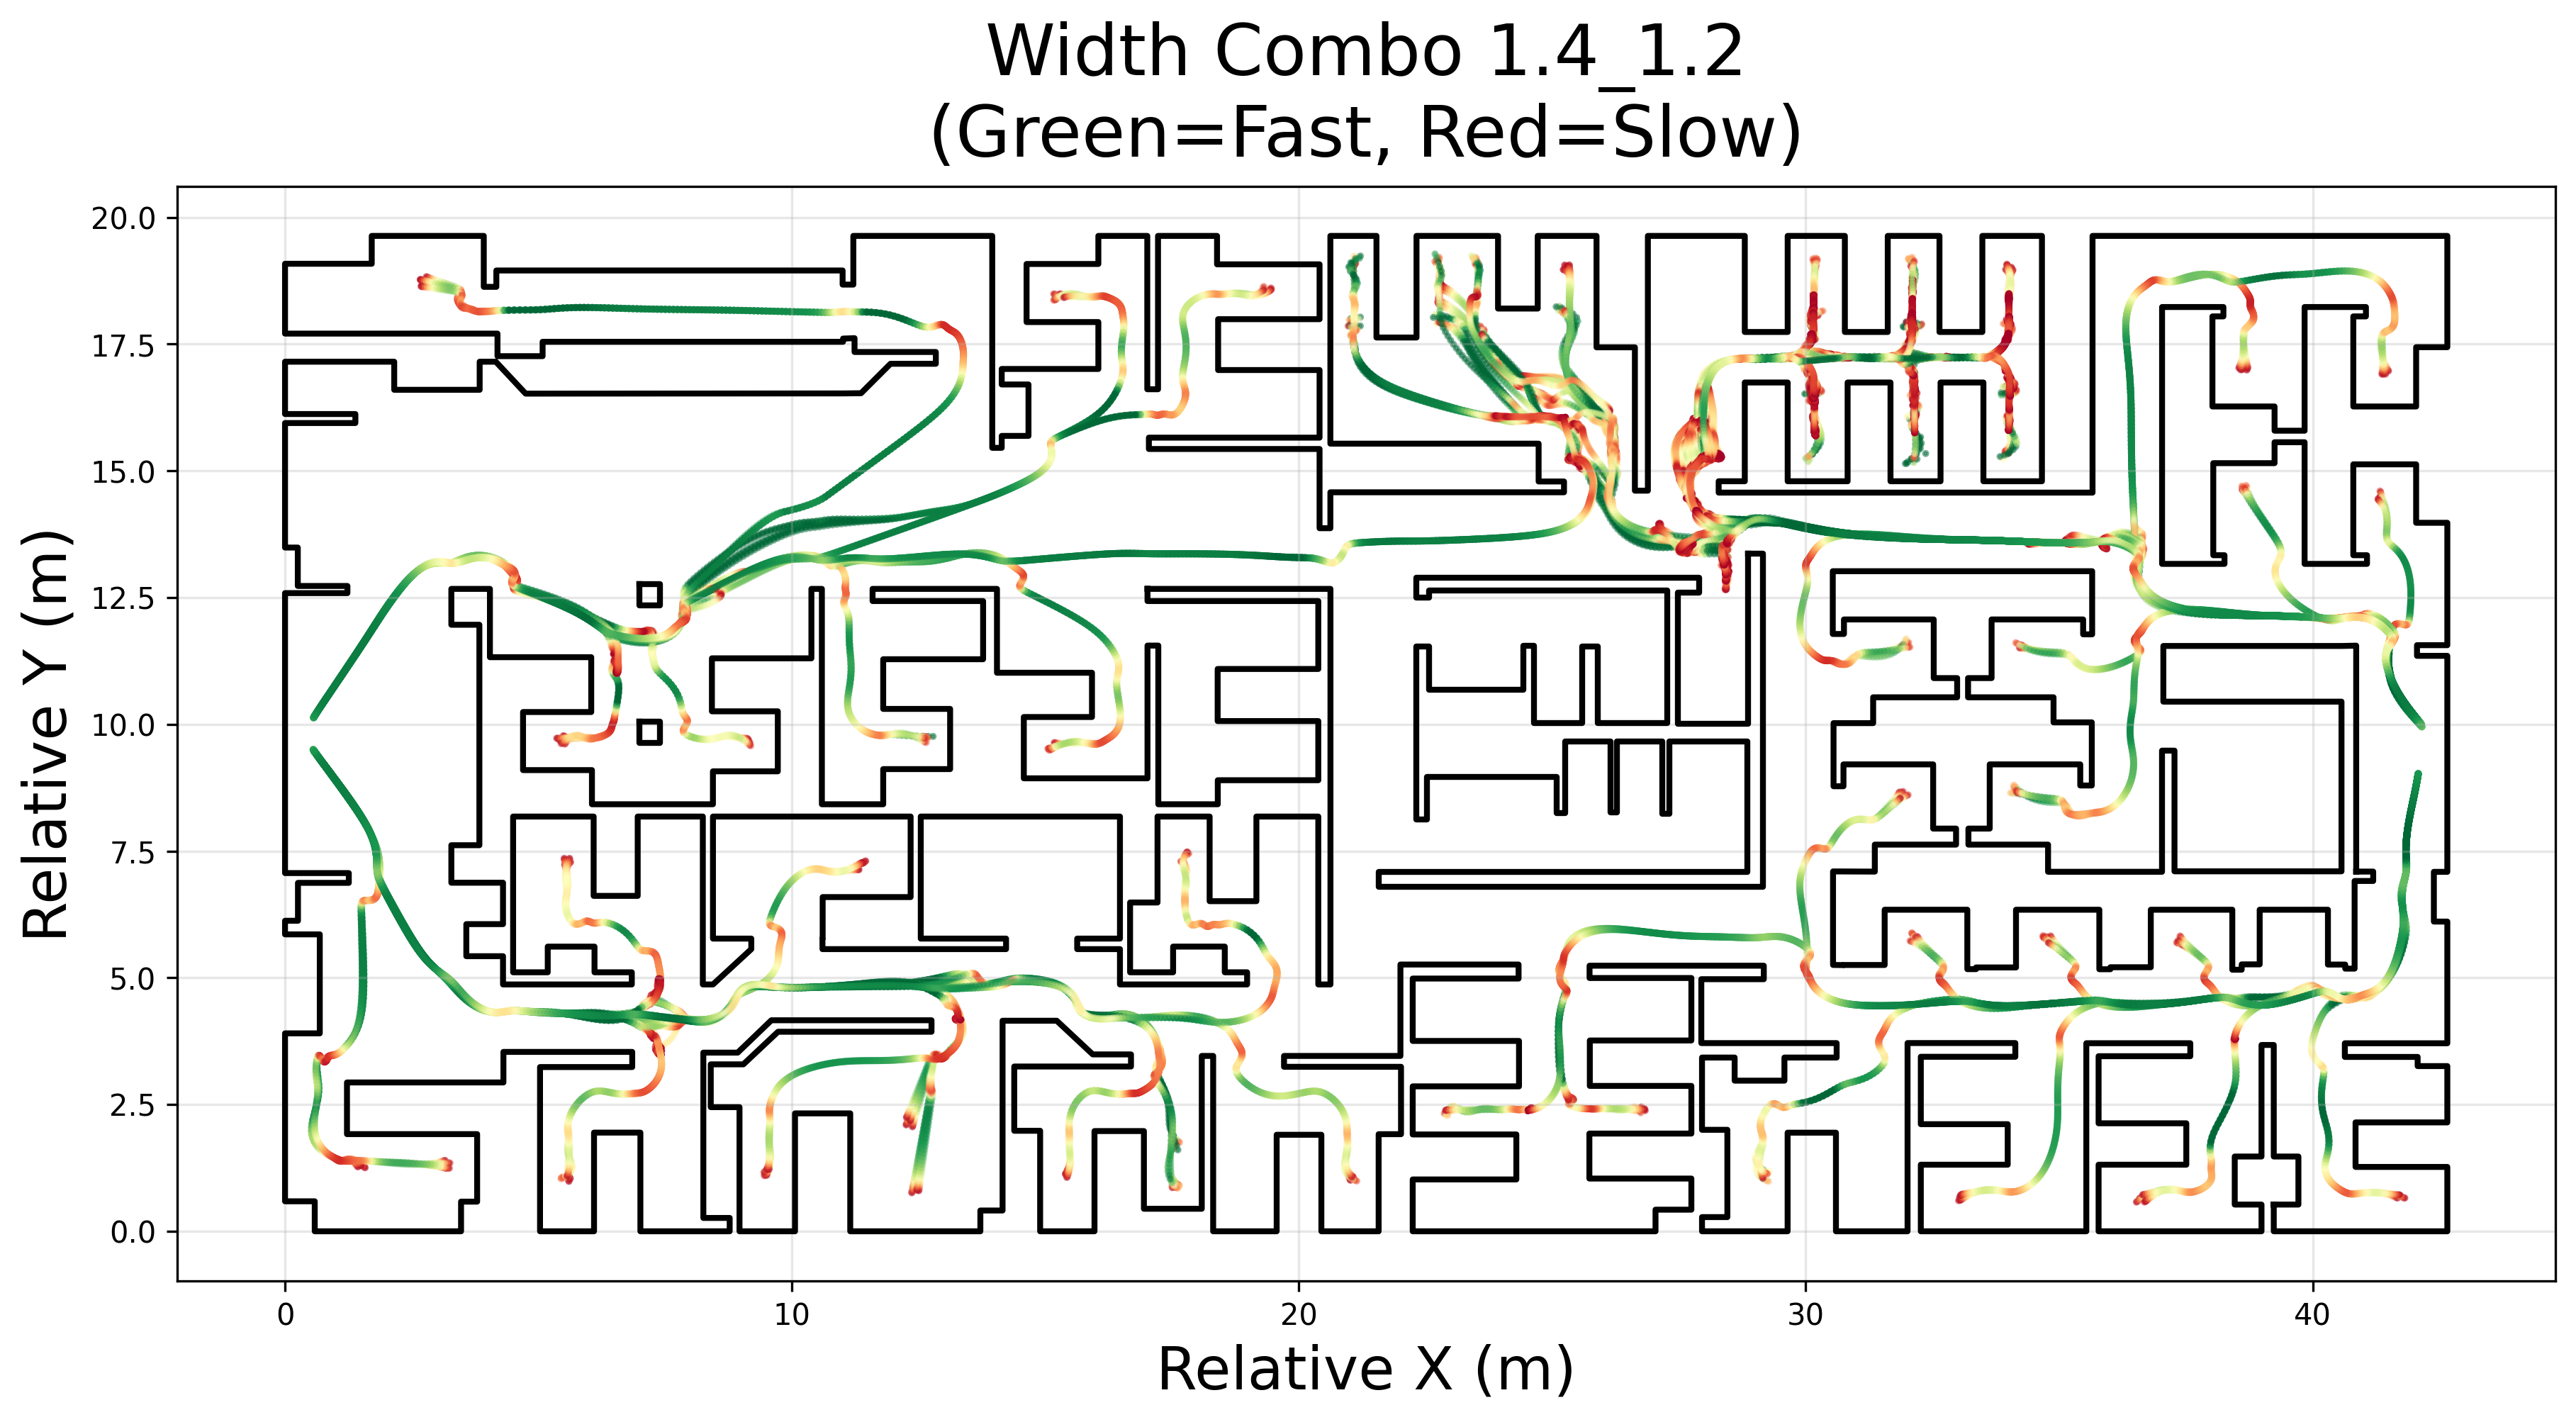
\includegraphics[width=\linewidth]{
            speed_trajectory_MultiRoom_width_1.4_1.2.png}
        \caption{Width Combo 1.4m and 1.2m}
        \label{fig:width_combo_1.4_1.2m}
    \end{subfigure}

    \begin{subfigure}[b]{.45\linewidth}
        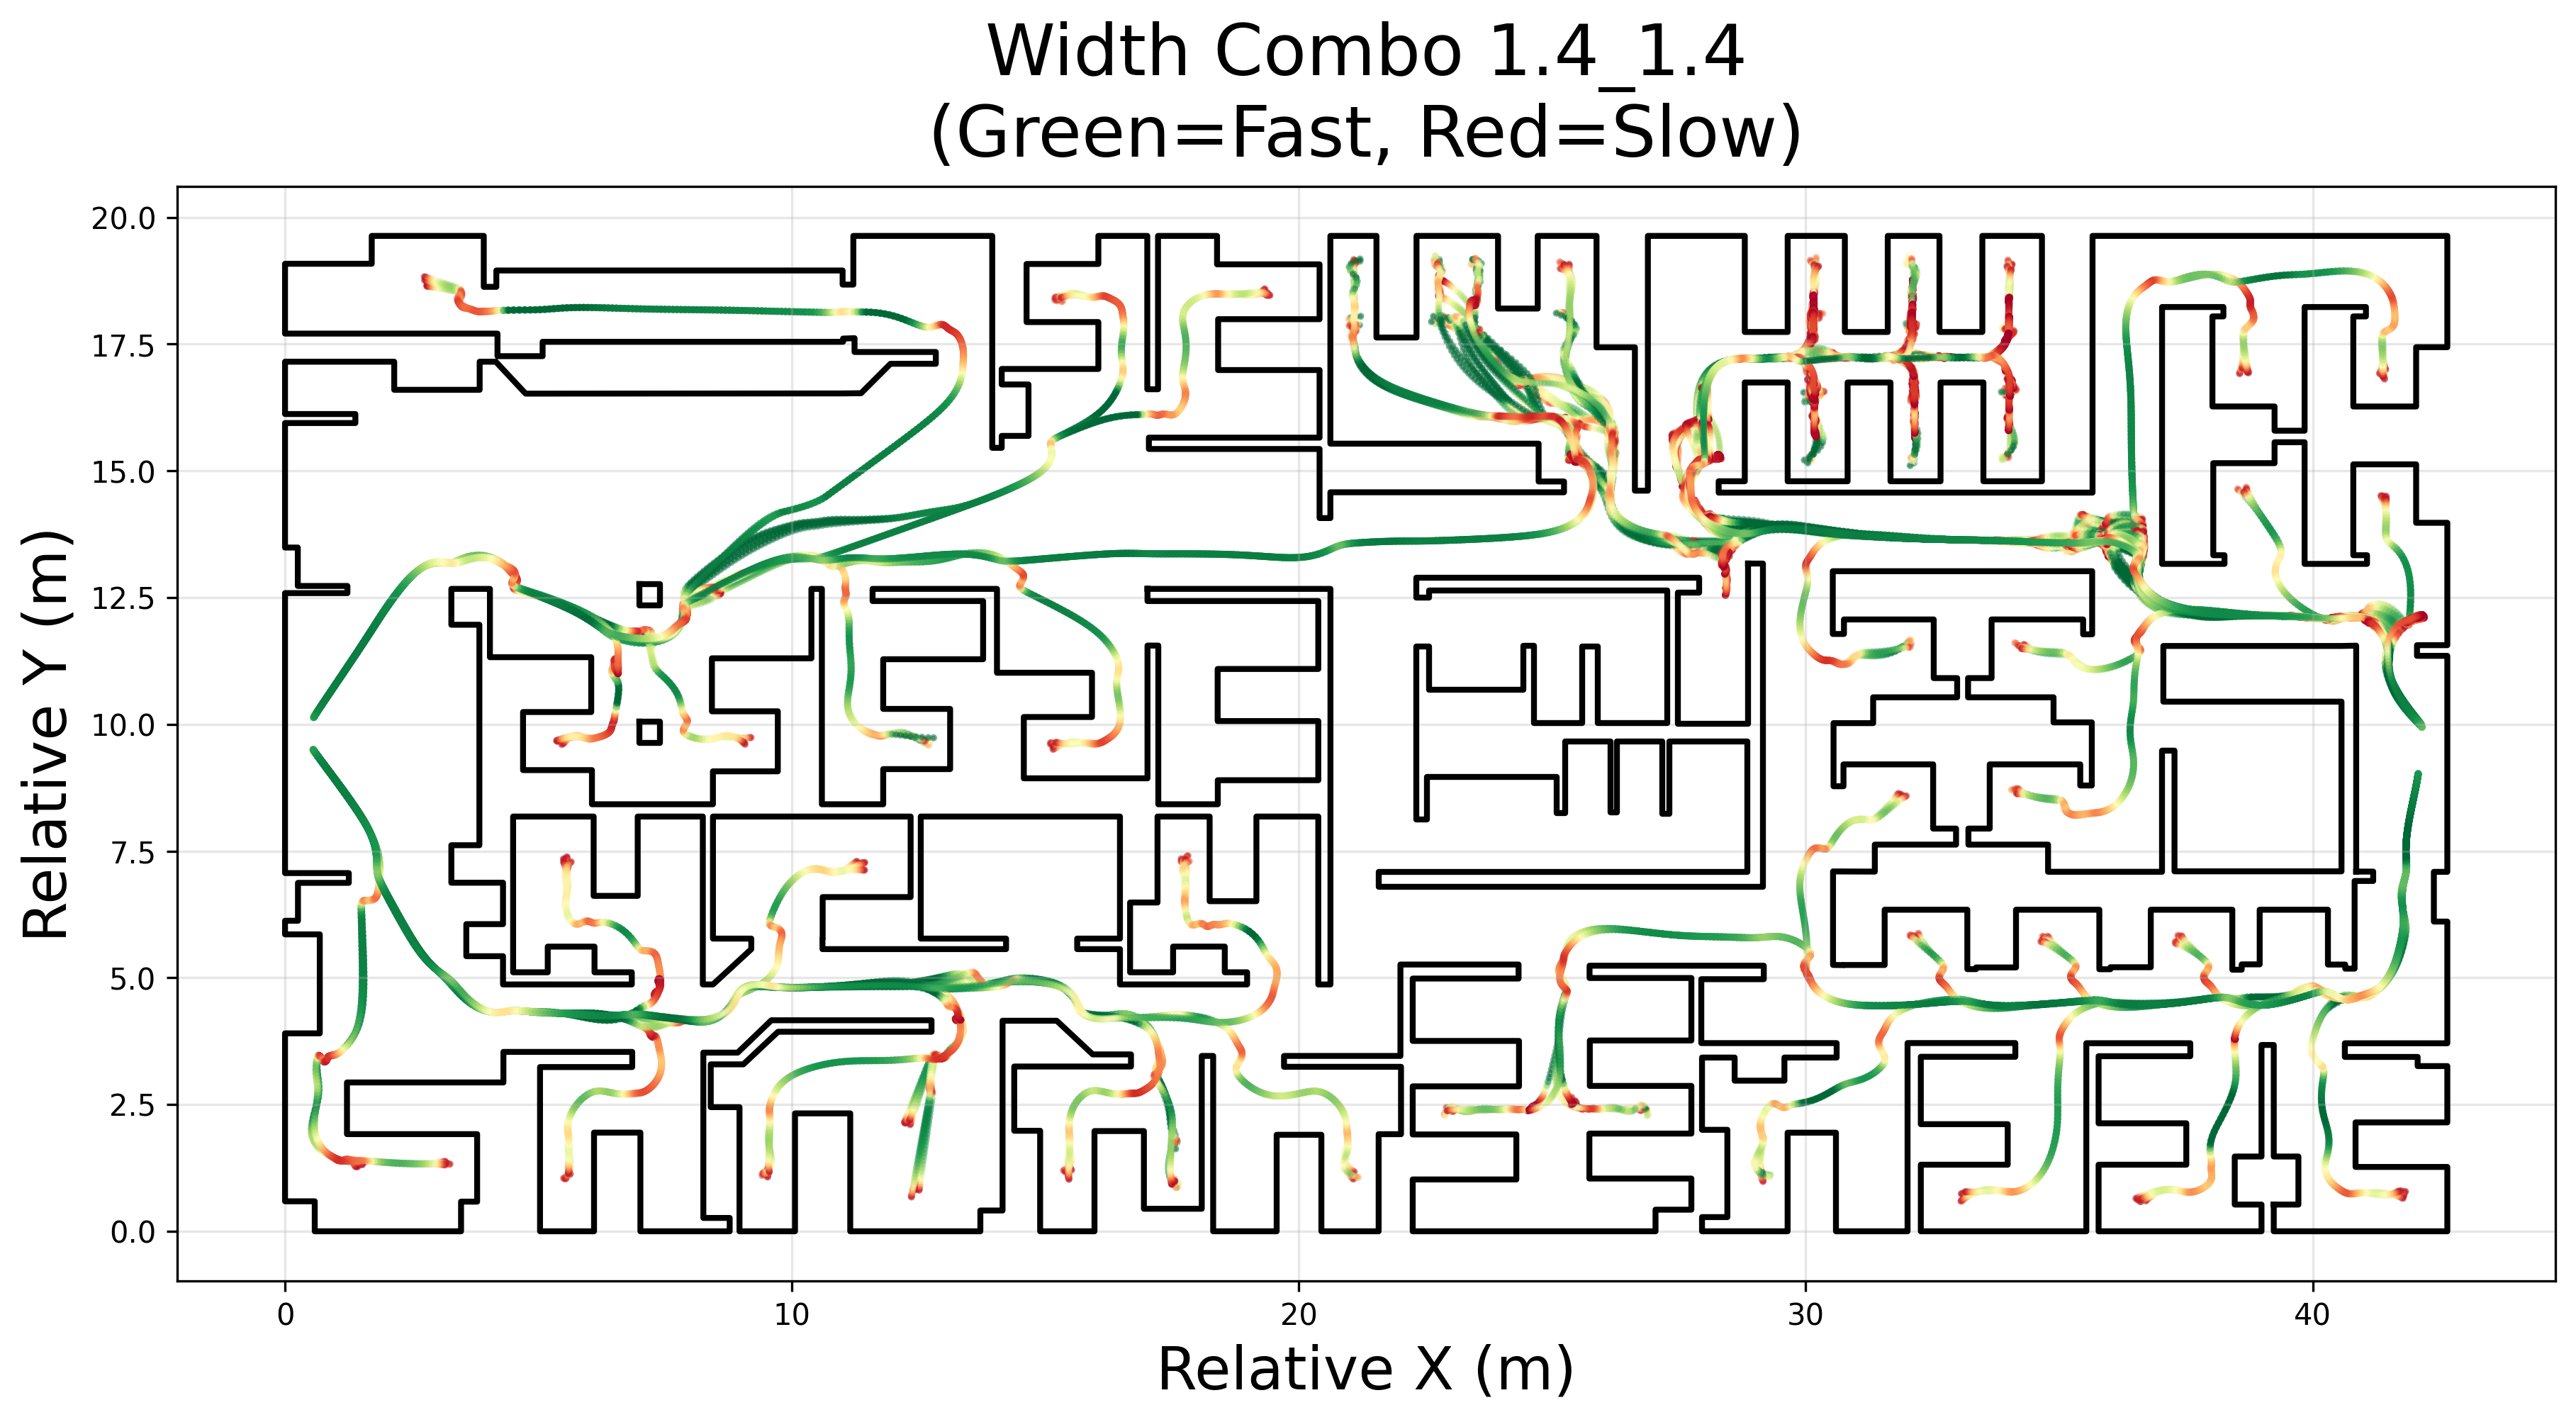
\includegraphics[width=\linewidth]{
            speed_trajectory_MultiRoom_width_1.4_1.4.png}
        \caption{Width Combo 1.4m and 1.4m}
        \label{fig:width_combo_1.4_1.4m}
    \end{subfigure}
    \begin{subfigure}[b]{.45\linewidth}
        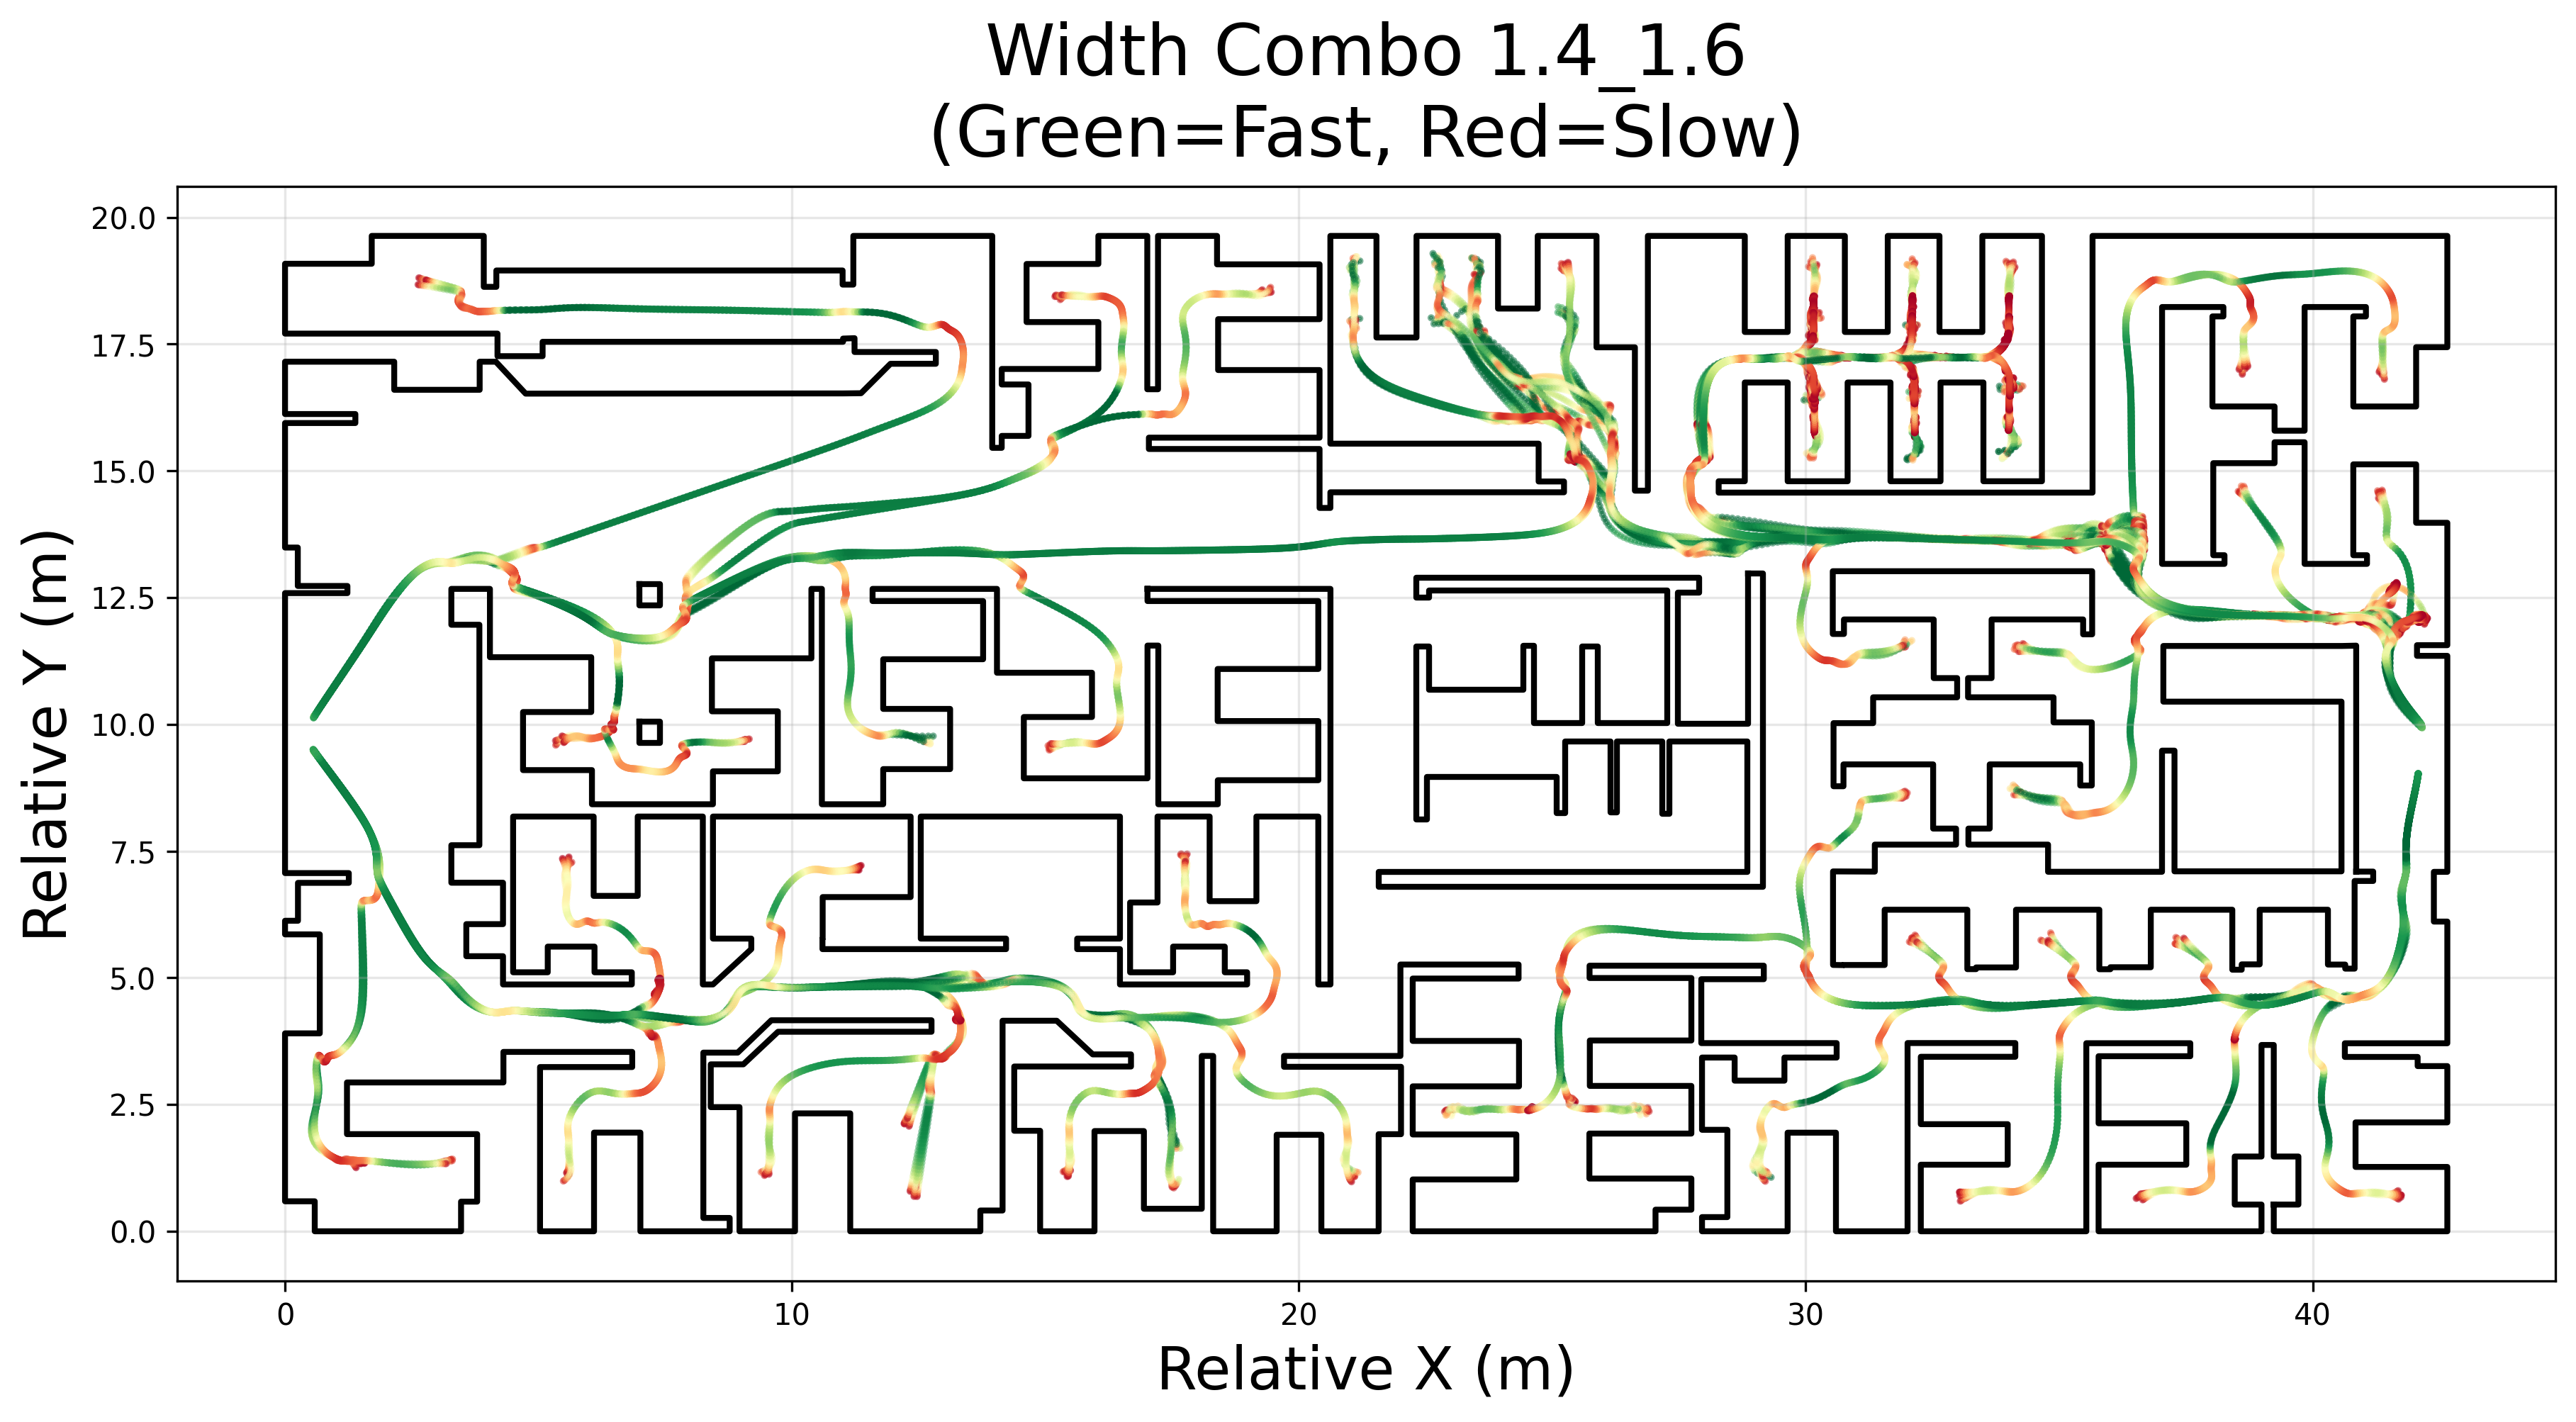
\includegraphics[width=\linewidth]{
            speed_trajectory_MultiRoom_width_1.4_1.6.png}
        \caption{Width Combo 1.4m and 1.6m}
        \label{fig:width_combo_1.4_1.6m}
    \end{subfigure}
    
    \caption{Speed and Trajectories for Room Door Width 1.4m}
    \label{fig:width_combo_1.4_x}
\end{figure}

For the case of 1.6m room door width \ref{fig:width_combo_1.6_x}, based on previous conclusions, the larger the room door, the greater the upstream supply of crowd, leading to more obvious congestion and normally resulting in higher evacuation times. What is interesting, under the same 1.0m corridor gate width condition (first column of the heat map \ref{fig:tet_vs_room_corridor_coupling}), the TET for the 1.6m \ref{fig:width_combo_1.6_1.0m} room door width is however lower than that \ref{fig:width_combo_1.4_1.0m} for the 1.4m one.

After reviewing the simulation playback, we discovered that the key lies in the differences in congestion patterns: under the 1.4 m room door width condition, it is more likely for four pedestrians to become mutually stuck \ref{fig:four_agents_stuck}, leading to flow interruption and significantly slowing down the overall evacuation. After we reviewed the TET from 5 simulations, the maximum was 98.7 s and the minimum was 84 s, showing a very large fluctuation range. Therefore, we can only preliminarily conclude that the 1.4 m room door width more easily triggers chaotic congestion patterns. This phenomenon further indicates that the influence of building geometric elements on evacuation time is highly complex, and specific conclusions still need to be verified through more experiments and large dataset in the future.

\begin{figure}
    \centering
    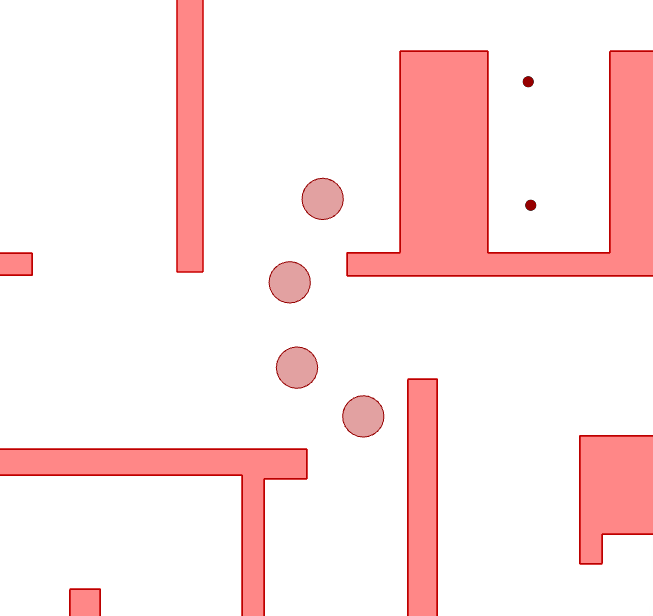
\includegraphics[width= 0.5 \linewidth]{FourAgentsStuck.png}
    \caption{Four Agents Stuck at the Corridor Gate}
    \label{fig:four_agents_stuck}
\end{figure}

\begin{figure}[h]
    \centering
        \begin{subfigure}[b]{.45\linewidth}
        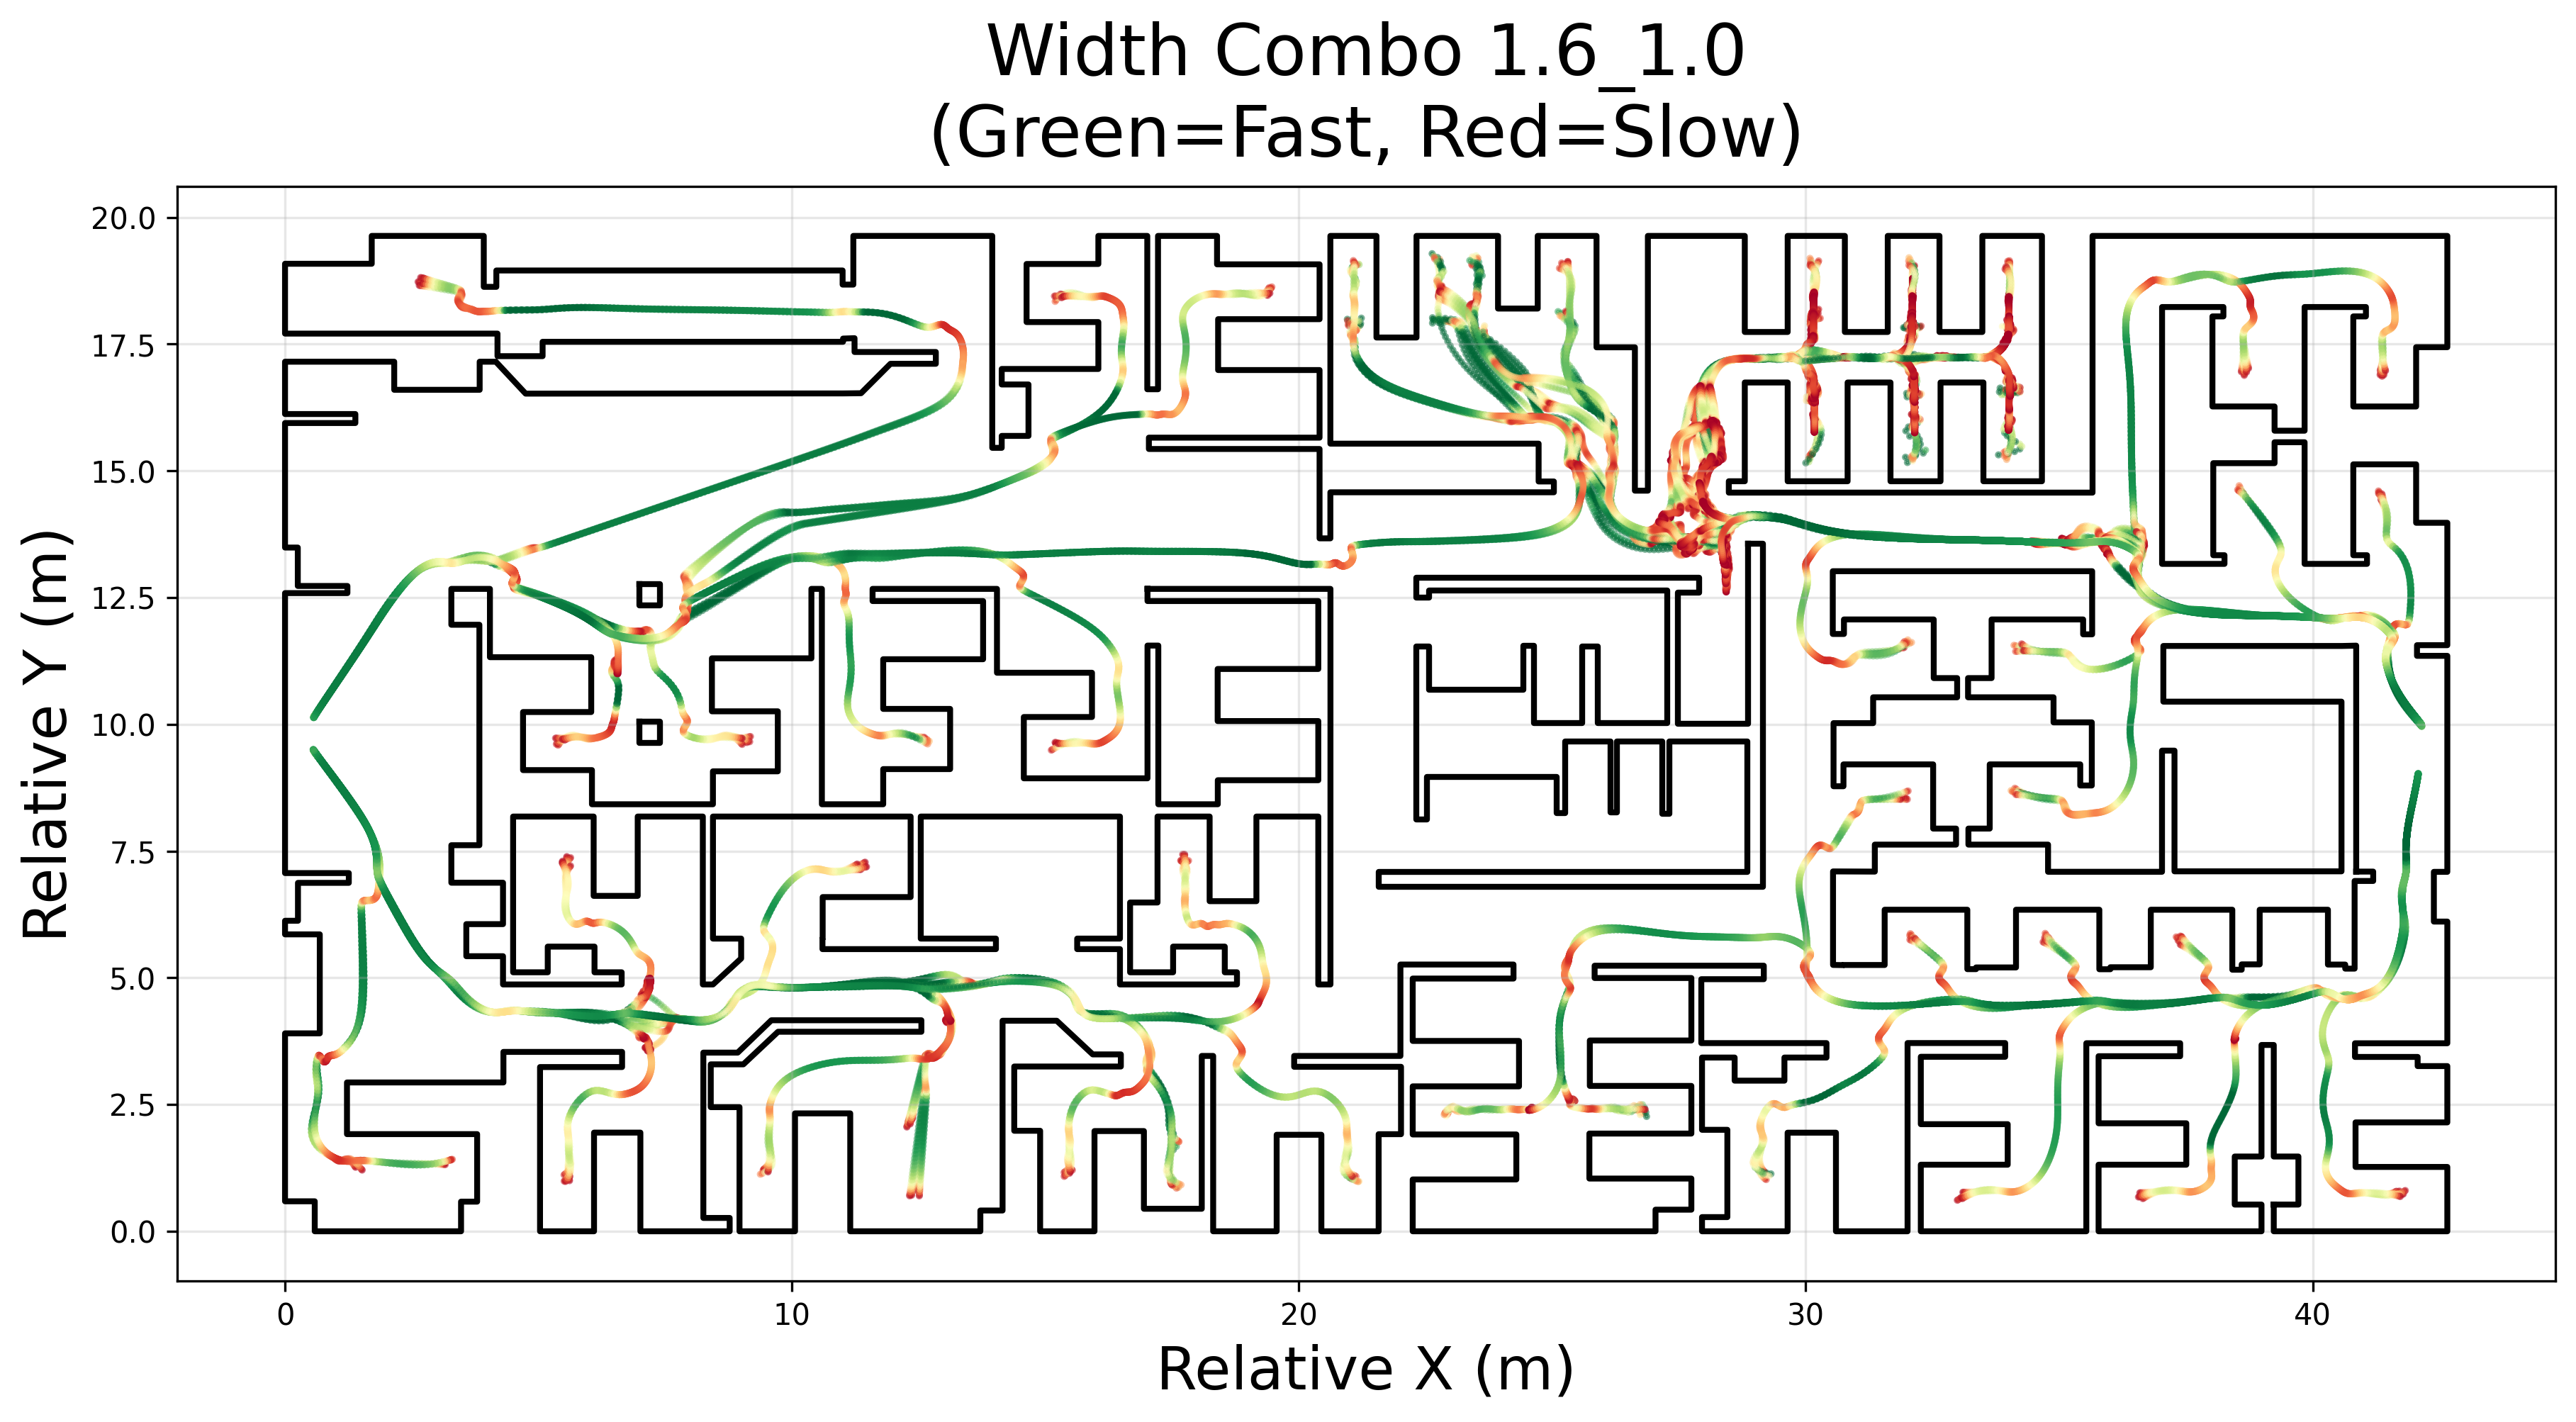
\includegraphics[width=\linewidth]{
            speed_trajectory_MultiRoom_width_1.6_1.0.png}
        \caption{Width Combo 1.6m and 1.0m}
        \label{fig:width_combo_1.6_1.0m}
    \end{subfigure}
    \begin{subfigure}[b]{.45\linewidth}
        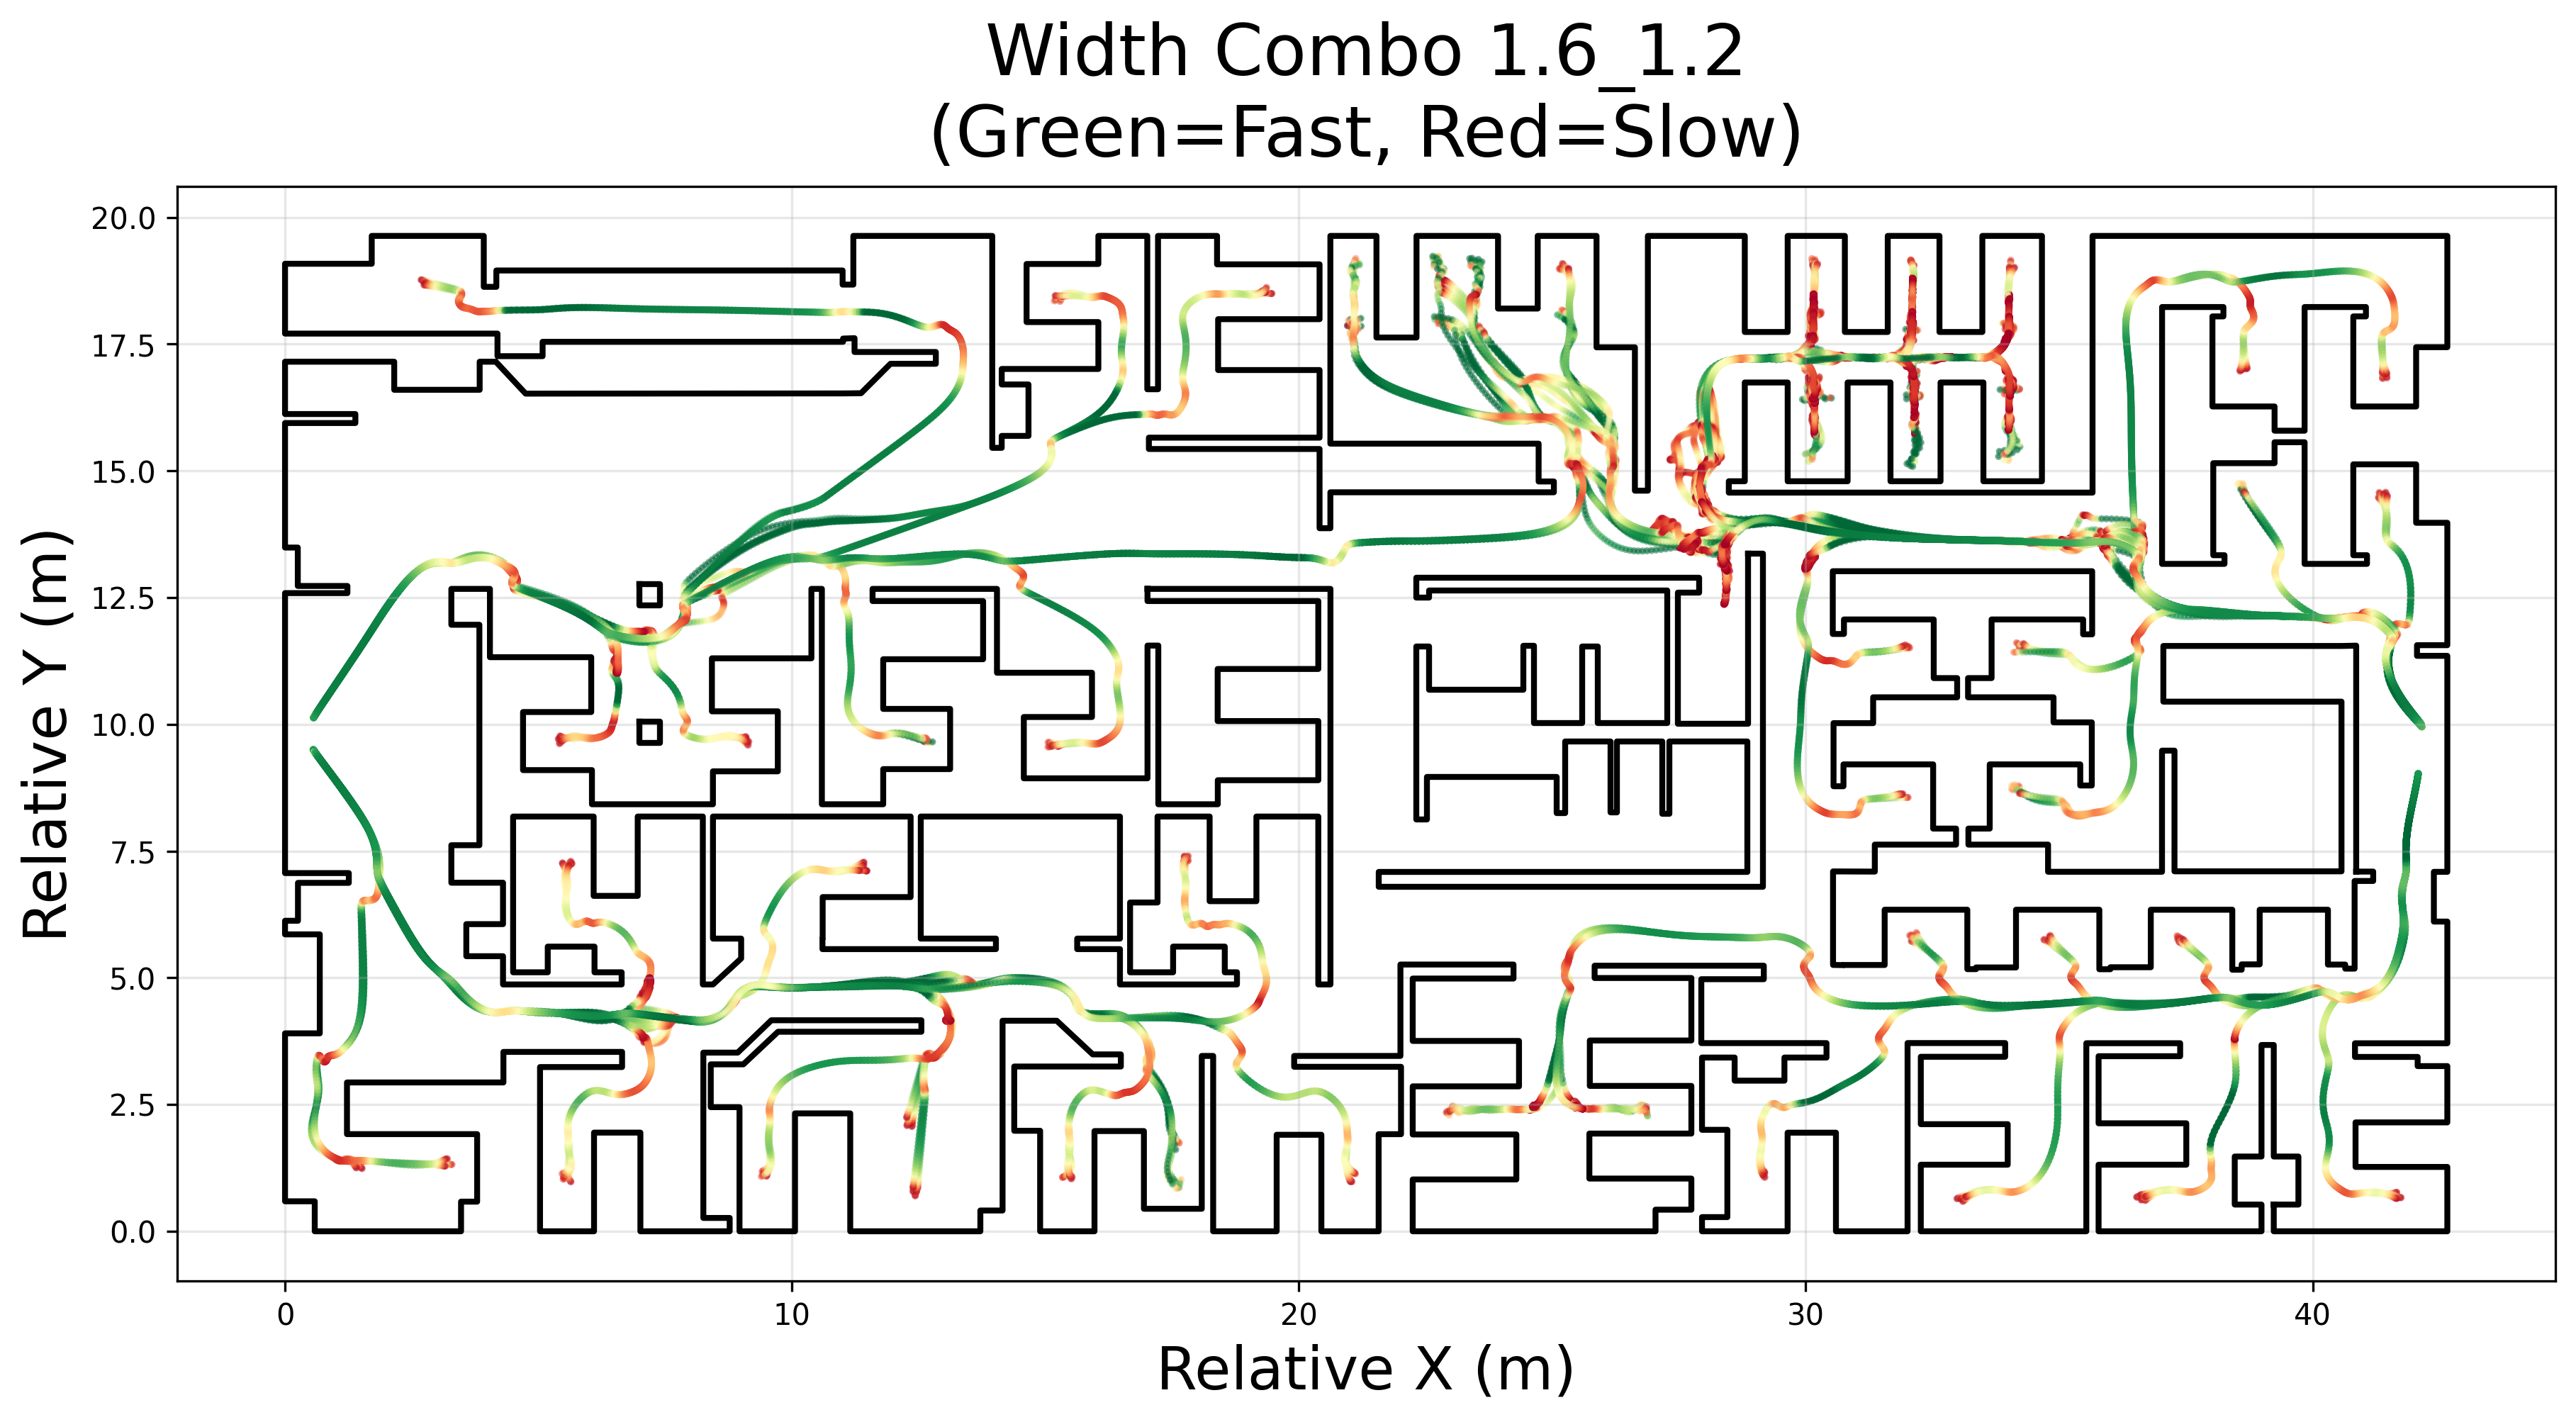
\includegraphics[width=\linewidth]{
            speed_trajectory_MultiRoom_width_1.6_1.2.png}
        \caption{Width Combo 1.6m and 1.2m}
        \label{fig:width_combo_1.6_1.2m}
    \end{subfigure}

    \begin{subfigure}[b]{.45\linewidth}
        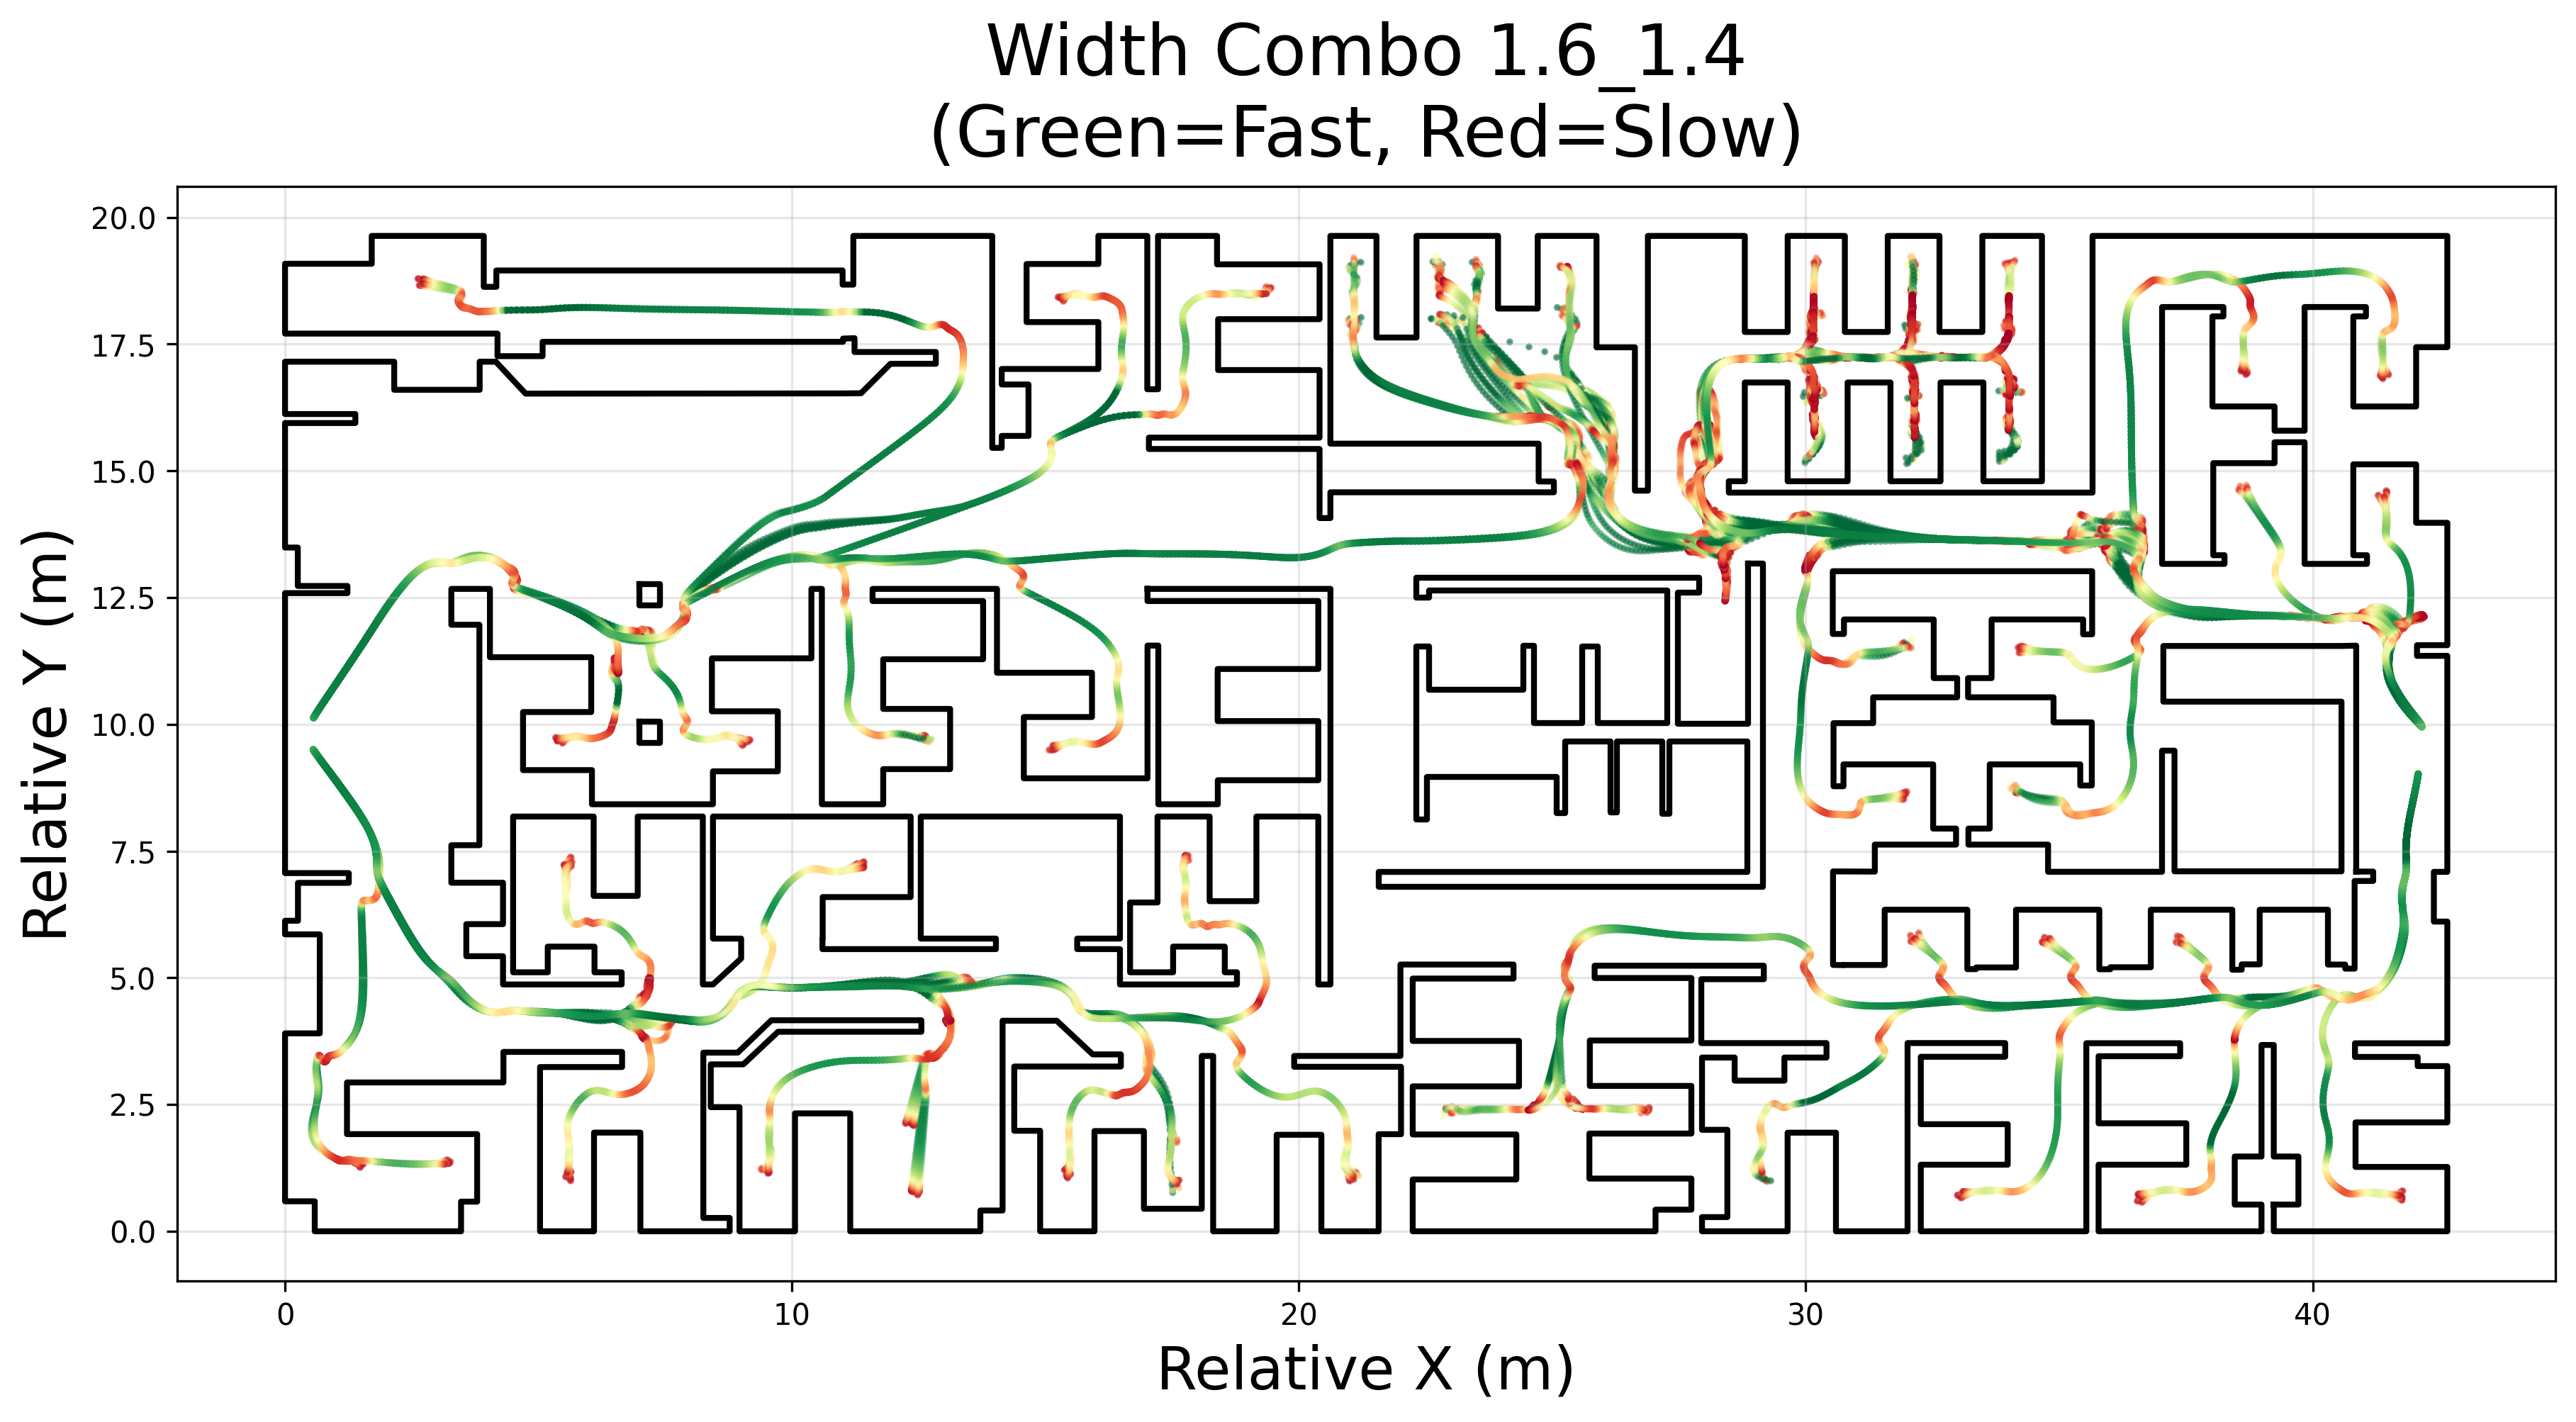
\includegraphics[width=\linewidth]{
            speed_trajectory_MultiRoom_width_1.6_1.4.png}
        \caption{Width Combo 1.6m and 1.4m}
        \label{fig:width_combo_1.6_1.4m}
    \end{subfigure}
        \begin{subfigure}[b]{.45\linewidth}
        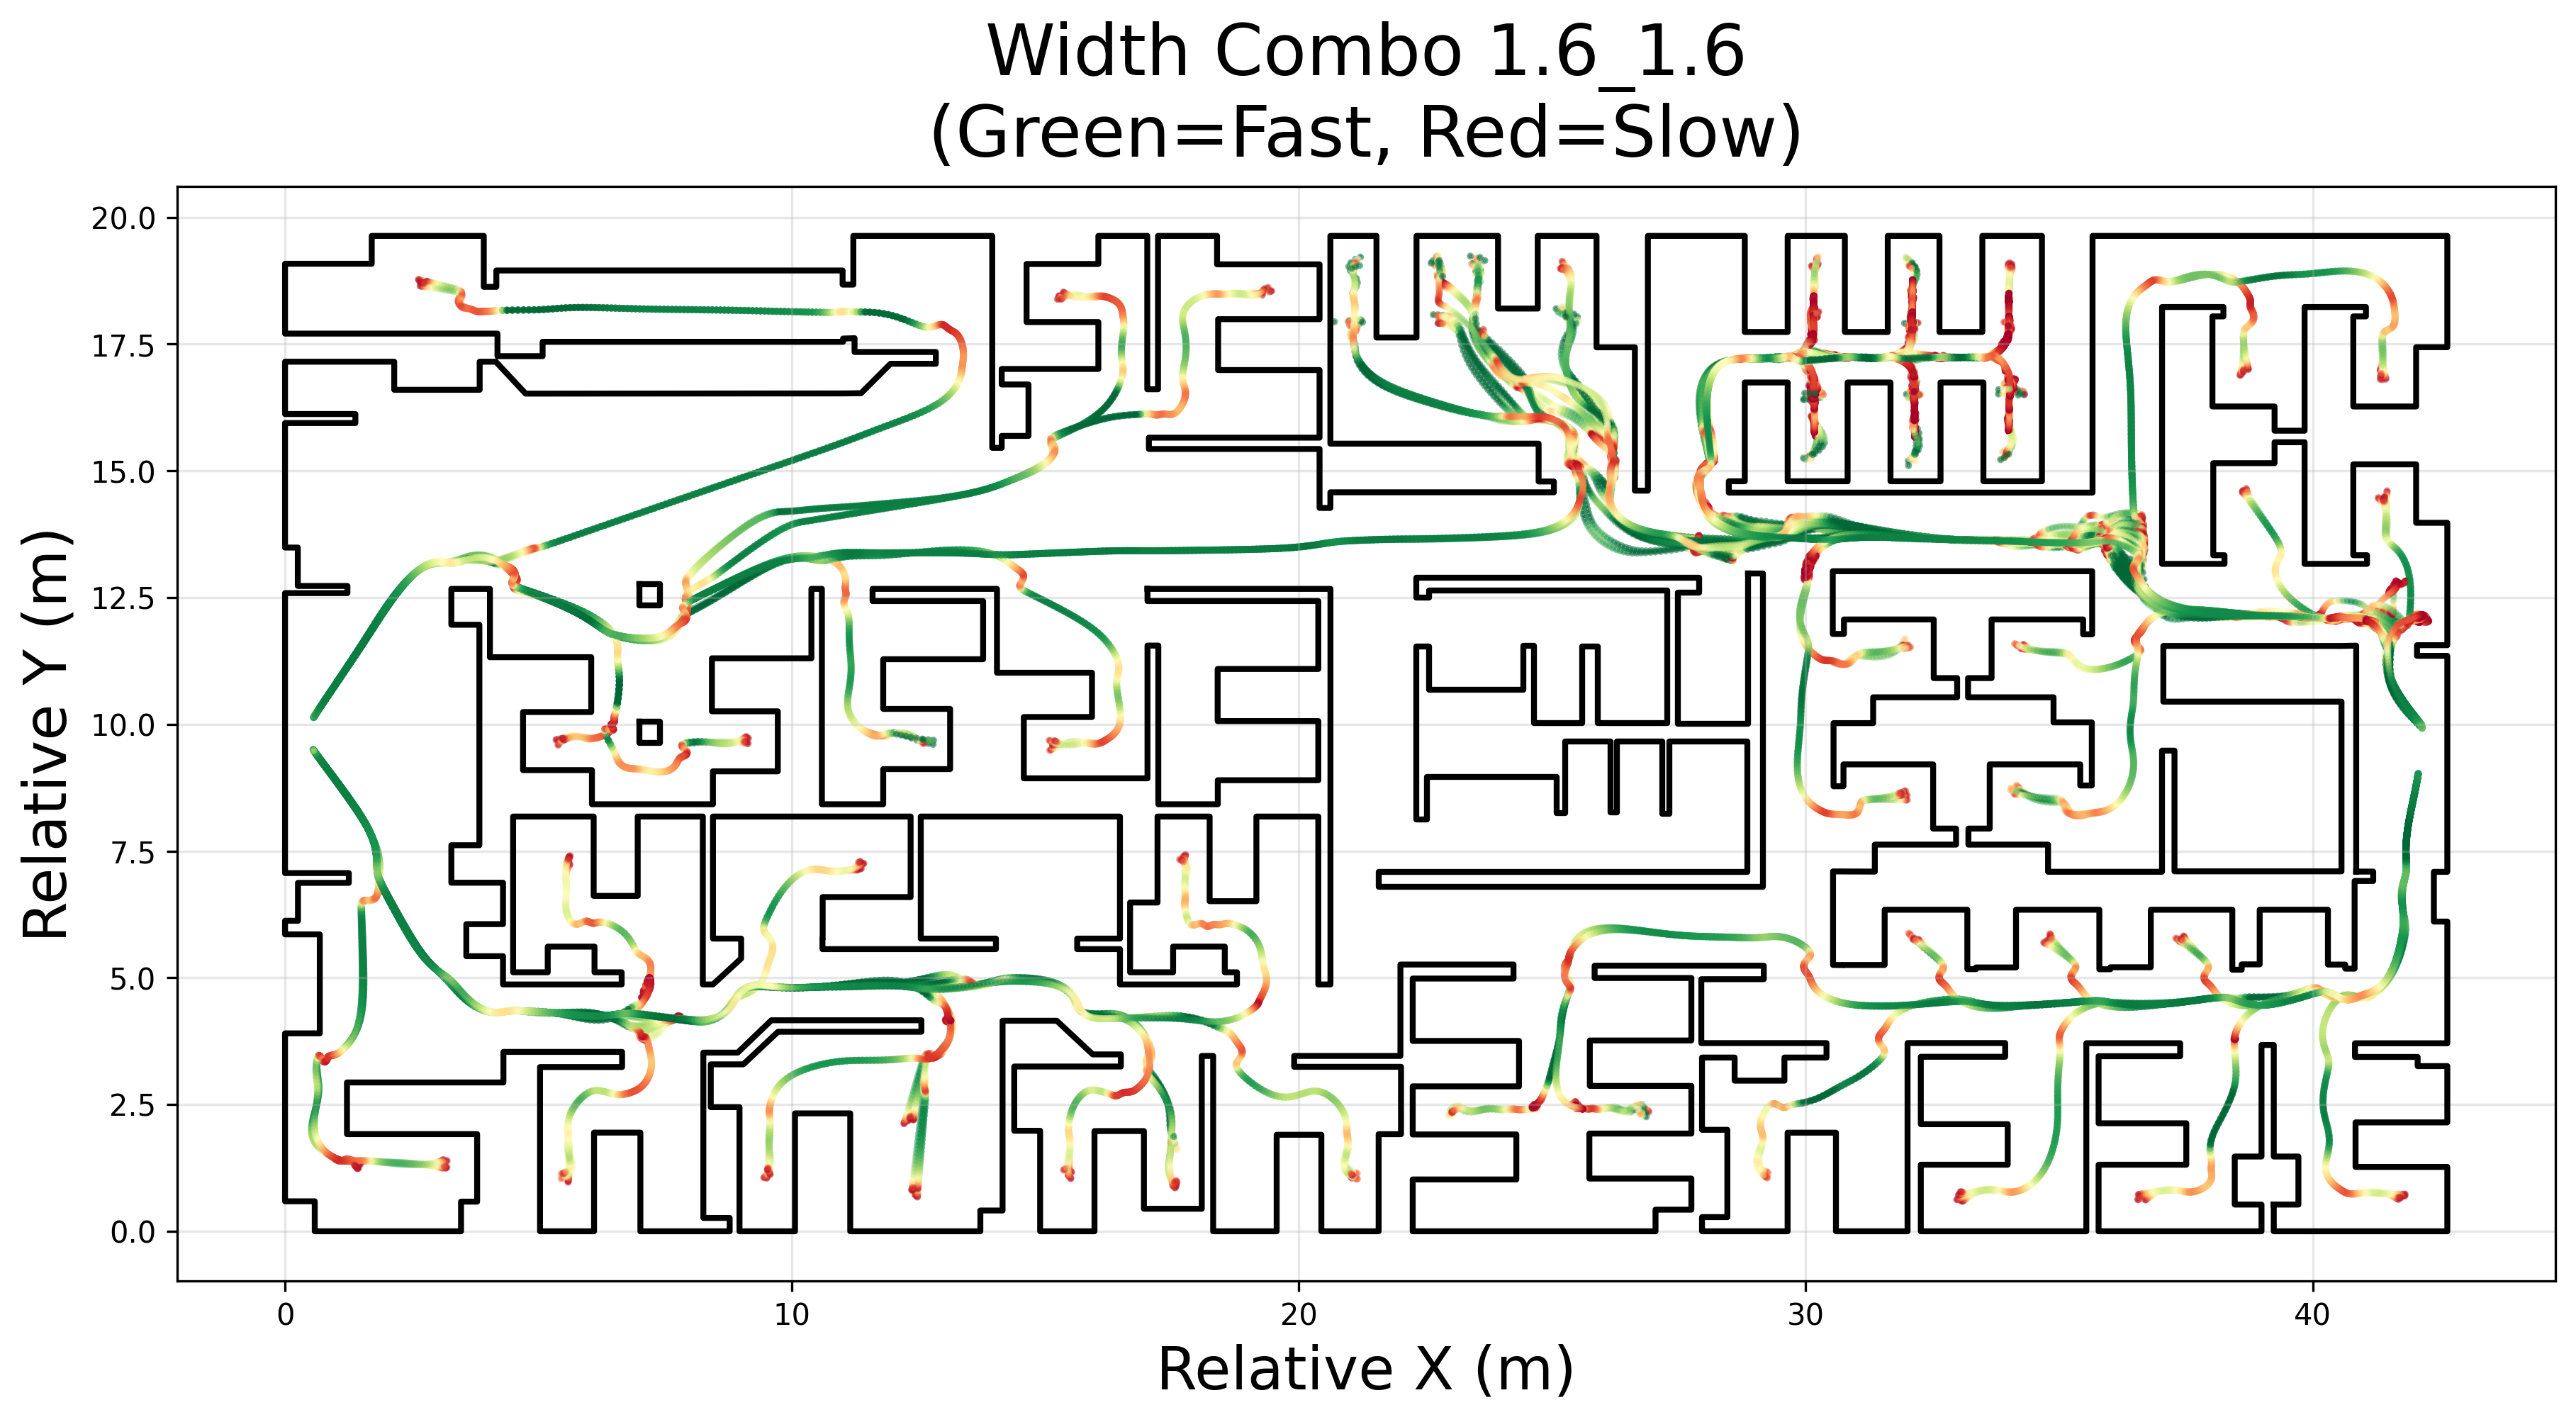
\includegraphics[width=\linewidth]{
            speed_trajectory_MultiRoom_width_1.6_1.6.png}
        \caption{Width Combo 1.6m and 1.6m}
        \label{fig:width_combo_1.6_1.6m}
    \end{subfigure}

    \caption{Speed and Trajectories for Room Door Width 1.6m}
    \label{fig:width_combo_1.6_x}
\end{figure}
%%%%%%

\chapter{Conclusion and Limitation}
\label{conclusionChapter}
\section{Social Force Model}
In simulations of emergency evacuation scenarios, researchers usually employ modeling methods such as social force models, cellular automata as well as agent-based models to simulate the complexity of crowd behavior. These models have become the primary approach in this field of study.
The social force model is an appealing method because it offers a relatively open and scalable framework. Compared to other models, the social force model can more intuitively explain the interactions between individuals and can replicate complex phenomena in crowded environments, such as speed, density and queuing situations. This model was first introduced by Helbing and Molnár in 1995, attempting to accurately simulate crowd behavior from a microscopic dynamics perspective, analogous to gas dynamics. Its core idea is to view crowd movement as a dynamic process influenced by various "forces".
Specifically, the social force model mainly considers four fundamental effects: (1) pedestrians wish to reach a specific destination; (2) pedestrians need to maintain a certain distance from each other; (3) pedestrians should keep a set distance from obstacles; (4) pedestrians may experience attraction towards specific objects (such as friends). Through the combined effects of these forces, the model can effectively explain the interactions among individuals and replicate complex phenomena in crowded environments.
Many researchers have continuously improved and applied the social force model, further expanding its potential. For example, Zheng and others combined the social force model with neural networks to simulate collective behavior in different scenarios; Seyfried and colleagues made modifications to pedestrian dynamics for qualitative analysis; Parisi and Dorso utilized this model to study the evacuation process in rooms with exits. These studies indicate that the social force model has become an important tool for simulating crowd movement, showing broad application prospects especially in areas like traffic planning and architectural design.

\section{Previous Work}
An important branch of evacuation simulation is the research on physical environmental factors. The key elements of spatial structure include the geometric form of buildings, exit configuration and the distribution of obstacles. The geometric form of buildings involves the shape of rooms, floor height and corridor width, and these parameters directly affect the possibility and efficiency of crowd movement. Exit configuration, including the number, location and width of exits, is a key factor in determining the evacuation speed. In addition, the distribution of obstacles, such as the spatial positions of fixed facilities like tables, chairs and columns, significantly affects the evacuation paths and crowd speeds .

In 2012, Ma et al. conducted experimental research on evacuation in China's skycrappers, focusing on the impact of building physical characteristics on the evacuation process. Peacock and Kuligowski (2004) systematically reviewed occupant movement in buildings and found that physical environment factors, including space configuration, exit placement, and obstacle distribution, significantly affect evacuation efficiency. Koo et al. (2013) compared evacuation strategies in high-rise buildings, particularly examining the paths of disabled individuals under different physical conditions. Their study revealed that the geometry and design of exits directly determine the feasibility and safety of evacuations. In high-density and emergency situations, these physical factors can greatly influence crowd behavior during evacuations. A common conclusion from these studies is that the physical environment is a significant influence on evacuation simulation, necessitating a comprehensive consideration of building shape, exit quantity and location, stair width, and obstacle distribution.

In research on classrooms and office spaces, while exit design is important, an increasing number of studies highlight the significant impact of internal furniture arrangement, desk layout, and corner configurations on evacuation efficiency. In some situations, these internal layout factors can outweigh the influence of exit width or quantity (Liu Parhizgar, 2018;). Helbing et al. specifically emphasized the considerable effect of obstacles, such as desks in a classroom, on evacuation efficiency. These findings indicate that optimizing layout by adjusting internal environmental parameters can significantly alter crowd path choices and congestion hotspots.

\section{Research Gap}
Despite the extensive research on evacuation simulations, there is still a lack of systematic exploration of how internal layout parameters affect evacuation performance in fixed structural settings. 

Firstly, existing studies lack a systematic analysis of how internal layout parameters interact. Most of the studies only focus on single parameter such as number of exits and layout of desks and seats, while ignoring factors including corners, corridor width and door width as well as their interaction, particularly in senarios with multiple exits and neted rooms.

Secondly, there is a lack of research on prototypes with different sizes. The lack of reliable methods for scaling from small and simple spaces to large and complex layout limits the translation of research results into practical applications.

Third, current research primarily focuses on simple scenarios such as classrooms, while systematic studies on the layout of office spaces are relatively scarce. Unlike traditional scenarios like classrooms, office spaces exhibit a high degree of complexity, including densely populated crowds, diverse furniture configurations, and dynamic layouts. The uniqueness of office spaces lies in the relatively fixed initial positions of personnel and the significant flexibility of furniture arrangements. Therefore, changes in the layout of office spaces may significantly impact evacuation efficiency, making them an ideal subject for evacuation simulation research.

Based on the aforementioned research limitations, the innovation of this study lies in: under the fixed structural constraints of office space scenarios, systematically comparing the evacuation performance of different scales and multiple layout variants, and revealing the coupling effects of door width, corridor width, and exit configuration through quantitative analysis. This research not only provides an actionable method for assessing the safety of office spaces but also offers a new methodological perspective for evacuation simulation studies.
%%%%%%

\chapter{Examples and Demos}
\label{examplesChapter}
So in here we will showcase the different things you can do.

\section{Citation}
\label{sec:citation}
We can cite things from the \emph{bib.tex} file using \verb=\cite{qdraw}= which will change into the appropriate citation style you chose \cite{qdraw}. "qdraw" is the \emph{Citation Key} set for that entry in Mendeley. You can also cite author, \citeauthor{qdraw}, in your text using \verb=\citeauthor{qdraw}=.

We can also cite other chapters, sections, figures, tables if they have a label. For example when we defined this section \verb=\section{Citation}= we added right after it a label \verb=\label{citationSection}= we can reference that section \ref{sec:citation} using \verb=\ref{sec:citation}=, you will notice "\ref{sec:citation}" is inserted and its also a hyperlink to the section.

\section{Labels}
Its best practice to start the labels with the type of objects:
\begin{itemize}
    \item \verb=\label{sec:FollowedWithSectionName}=
    \item \verb=\label{tab:FollowedWithTableName}=
    \item \verb=\label{fig:FollowedWithFigureName}=
    \item \verb=\label{lis:FollowedWithListingName}=
    \item \verb=\label{ch:FollowedWithChapterName}=
\end{itemize}

\section{Adding a SVG}
Using this template you can add an svg figure from your \emph{fig} folder. Inkscape needs to be installed, in the background Inkscape will be run to convert your SVG to a PDF, it will get placed in a folder in the root folder called \emph{svg-inkscape} and used.

\begin{Verbatim}[fontsize=\relsize{-1.5}]
    \begin{figure}[h]
        \centering
        \includesvg[width = 0.25\textwidth]{Firefox}
        \caption{This is a SVG logo.}
        \label{fig:svglogo}
    \end{figure}
\end{Verbatim}

\begin{figure}[h]
    \centering
    \includesvg[width = 0.25\textwidth]{Firefox}
    \caption{This is a SVG logo.}
    \label{fig:svglogo}
\end{figure}
%\pagebreak
\section{Adding an Image}
Its very similar to the SVG. Since in the \emph{Main.tex} file we already set our Graphics Path \verb=\graphicspath{{fig/}}=, we can write directly the name of an image or a folder inside that.
\begin{Verbatim}[fontsize=\relsize{-1.5}]
    \begin{figure}[h]
        \centering
        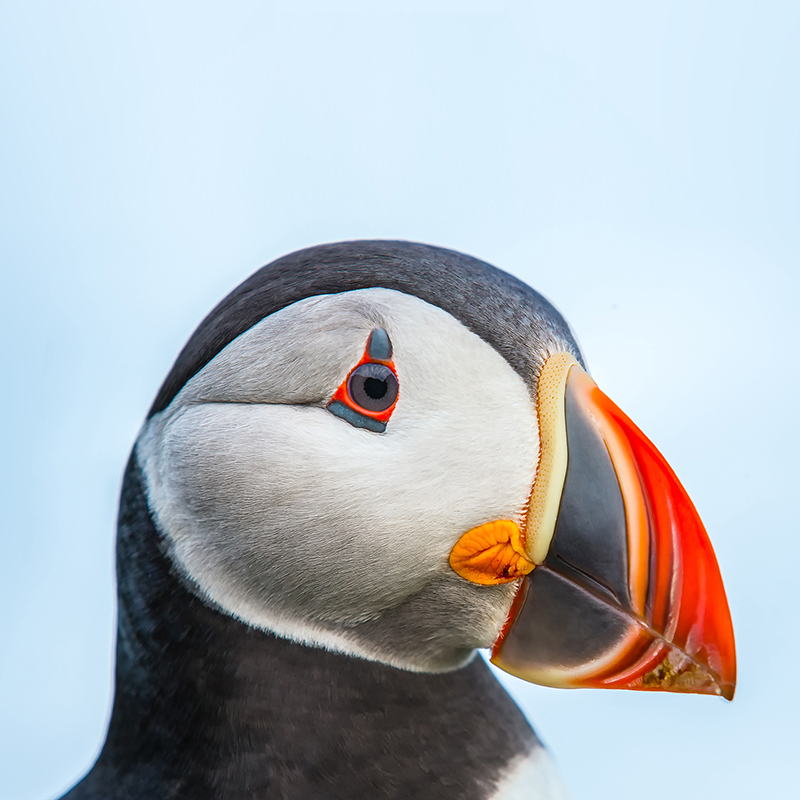
\includegraphics[width=\textwidth]{puffin}
        \caption{This is a puffin...}
        \label{fig:puffin}
    \end{figure}
\end{Verbatim}
\begin{figure}[h]
    \centering
    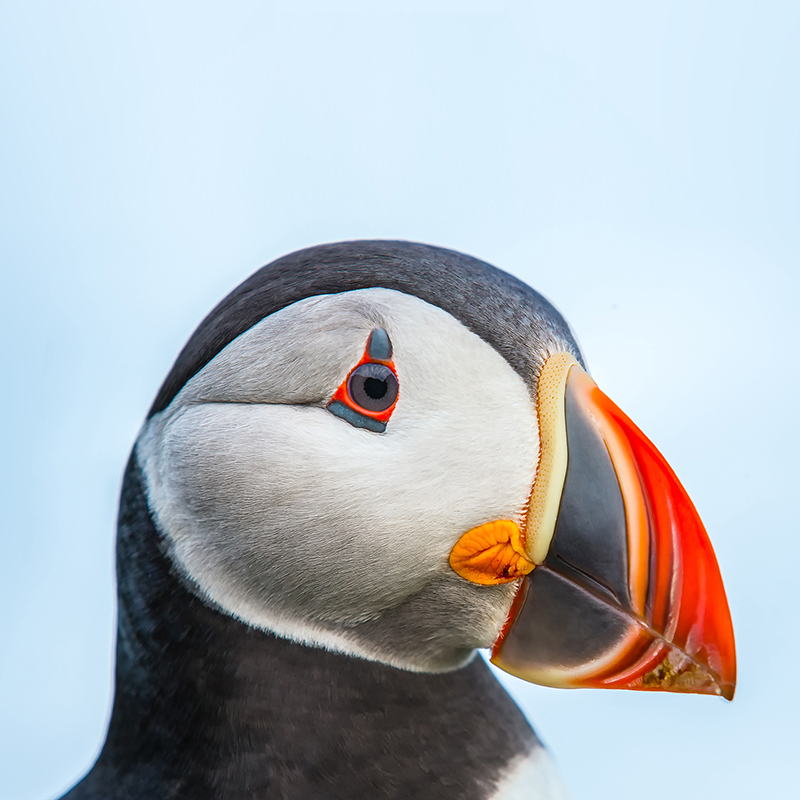
\includegraphics[width=\textwidth]{puffin}
    \caption{This is a puffin...}
    \label{fig:puffin}
\end{figure}

\faWarning\, If you go back to List of Figures, you will notice the two figures we just created were added automatically.

\faWarning\, If you noticed with the SVG and the image we used \verb_width=\textwidth_ using text width allows us to  easily stretch the image to the same width of our text.

\faWarning\, Use \verb=\ref{fig:puffin}= and \verb=\ref{fig:svglogo}= to refer to figure \ref{fig:puffin} and figure \ref{fig:svglogo}.
\pagebreak
\subsection{Multiple images}
You can insert images in a grid. For this we are using the \emph{Subcaption} package. The idea is to use a \emph{subfigure} with a width less than $linewidth$. Check here \url{http://mirrors.ibiblio.org/CTAN/macros/latex/contrib/caption/subcaption.pdf} and here \url{https://tex.stackexchange.com/a/119985} for details.
\begin{Verbatim}[fontsize=\relsize{-1.5}]
    \begin{figure} [H]
        \centering
        \begin{subfigure}[b]{.45\linewidth}
            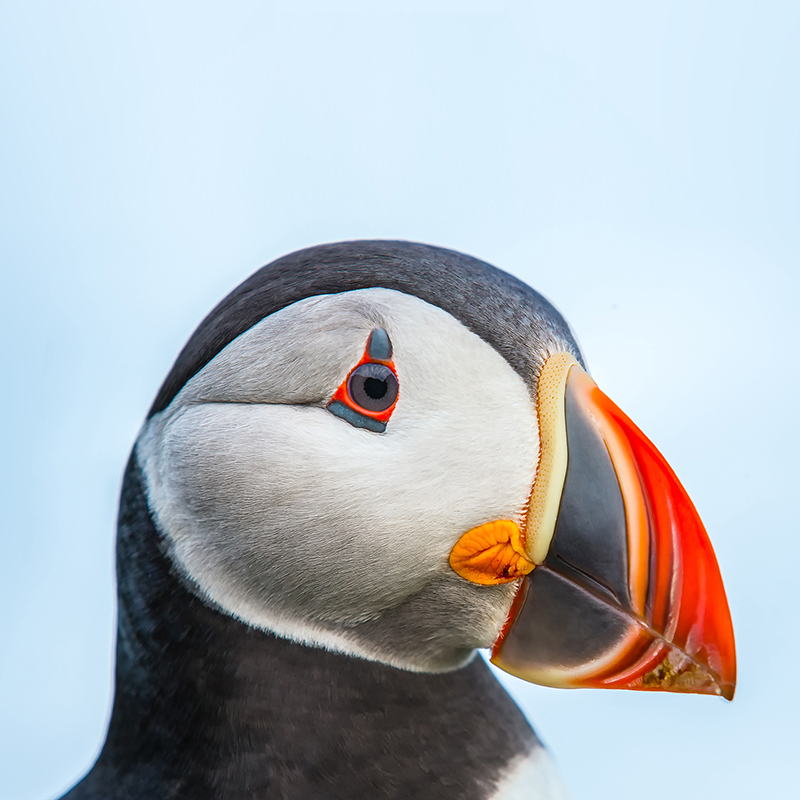
\includegraphics[width=\linewidth]{puffin}
            \caption{Useless Image}\label{fig:puffin1}
        \end{subfigure}
        \begin{subfigure}[b]{.45\linewidth}
            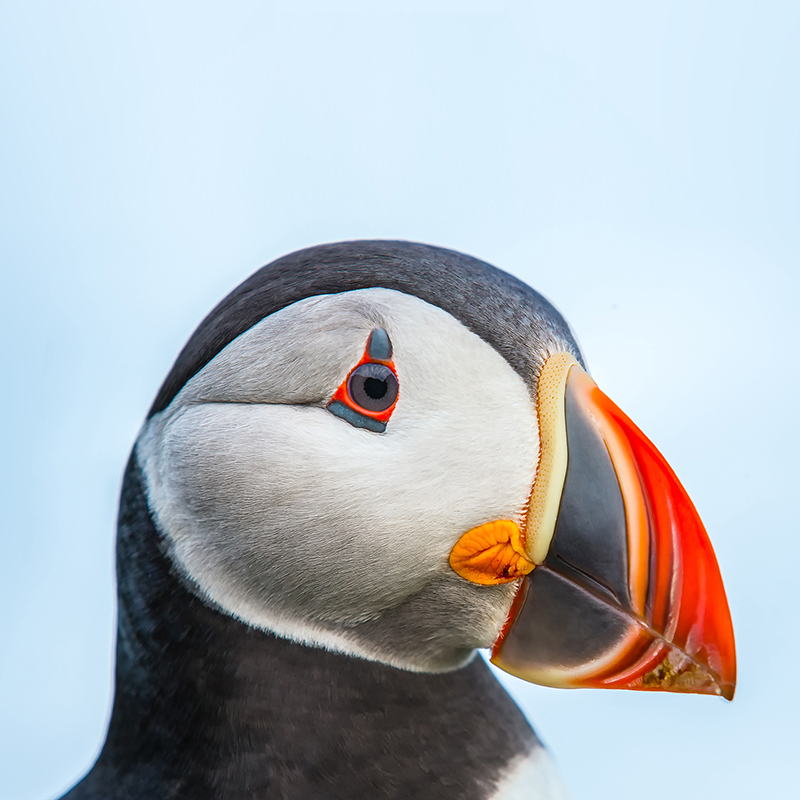
\includegraphics[width=\linewidth]{puffin}
            \caption{puffin Image}\label{fig:puffin2}
        \end{subfigure}

        \begin{subfigure}[b]{.45\linewidth}
            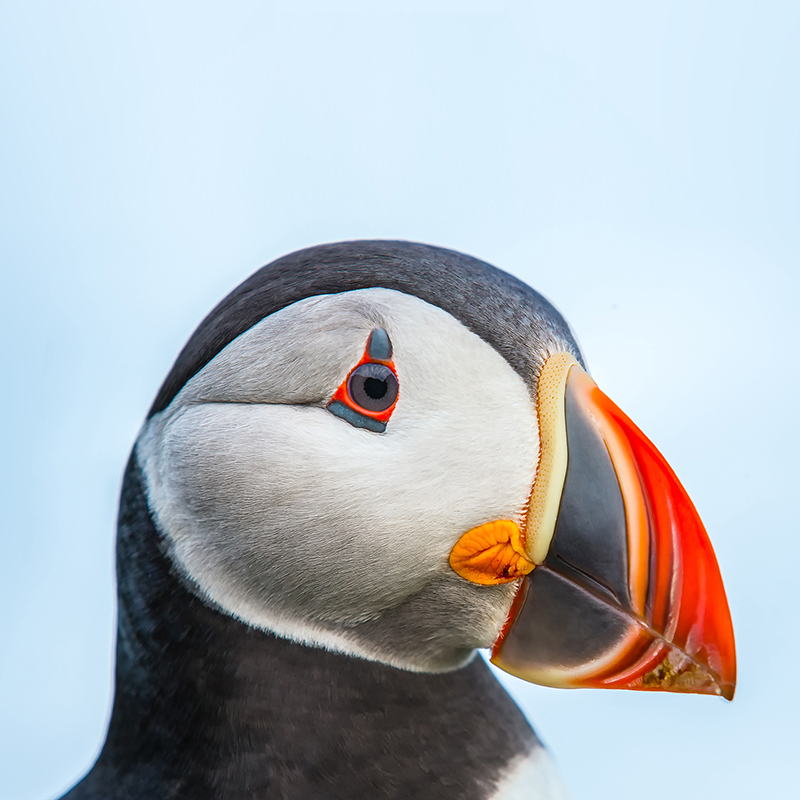
\includegraphics[width=\linewidth]{puffin}
            \caption{puffin Image}\label{fig:puffin4}
        \end{subfigure}
        \begin{subfigure}[b]{.45\linewidth}
            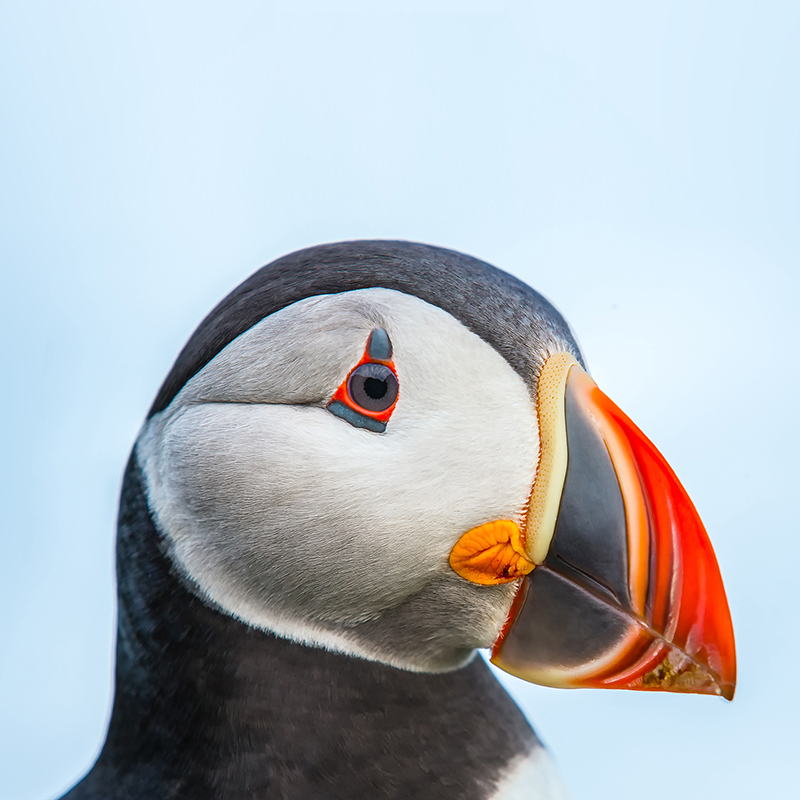
\includegraphics[width=\linewidth]{puffin}
            \caption{puffin Image}\label{fig:puffin5}
        \end{subfigure}

        \begin{subfigure}[b]{.45\linewidth}
            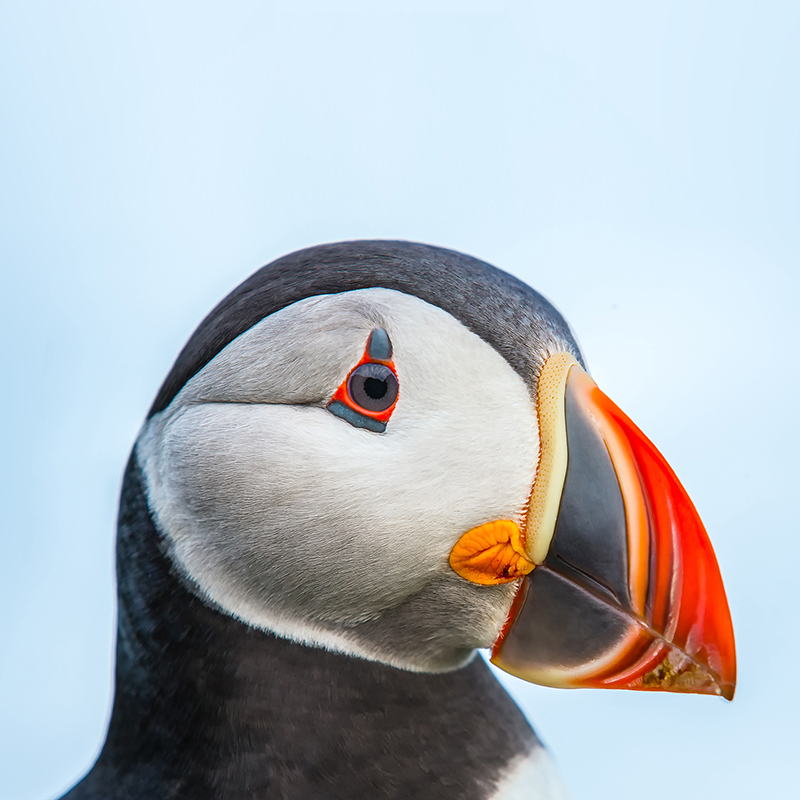
\includegraphics[width=\linewidth]{puffin}
            \caption{puffin Image}\label{fig:puffin6}
        \end{subfigure}
        \begin{subfigure}[b]{.45\linewidth}
            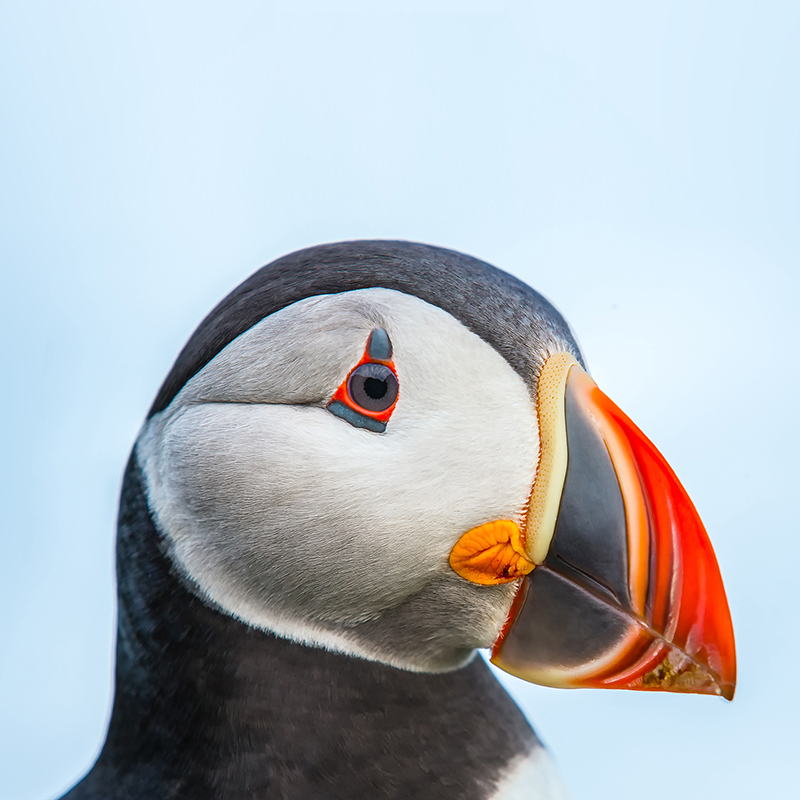
\includegraphics[width=\linewidth]{puffin}
            \caption{puffin Image}\label{fig:puffin7}
        \end{subfigure}
        \caption{A sample of multiple puffins}
        \label{fig:puffinall}
    \end{figure}
\end{Verbatim}
\begin{figure} [H]
    \centering
    \begin{subfigure}[b]{.45\linewidth}
        \includegraphics[width=\linewidth]{puffin}
        \caption{Useless Image}\label{fig:puffin1}
    \end{subfigure}
    \begin{subfigure}[b]{.45\linewidth}
        \includegraphics[width=\linewidth]{puffin}
        \caption{puffin Image}\label{fig:puffin2}
    \end{subfigure}

    \begin{subfigure}[b]{.45\linewidth}
        \includegraphics[width=\linewidth]{puffin}
        \caption{puffin Image}\label{fig:puffin4}
    \end{subfigure}
    \begin{subfigure}[b]{.45\linewidth}
        \includegraphics[width=\linewidth]{puffin}
        \caption{puffin Image}\label{fig:puffin5}
    \end{subfigure}

    \begin{subfigure}[b]{.45\linewidth}
        \includegraphics[width=\linewidth]{puffin}
        \caption{puffin Image}\label{fig:puffin6}
    \end{subfigure}
    \begin{subfigure}[b]{.45\linewidth}
        \includegraphics[width=\linewidth]{puffin}
        \caption{puffin Image}\label{fig:puffin7}
    \end{subfigure}
    \caption{A sample of multiple puffins}
    \label{fig:puffinall}
\end{figure}
\faWarning\, Notice here we used \verb=\subsection{Multiple images}= to create this subsection.
\subsection{Wrapped Images}
\begin{wrapfigure}{r}{0.35\textwidth}
    \centering
    \includegraphics[width=0.3\textwidth]{puffin.jpg}
\end{wrapfigure}
You can place images next to text. For this we are using the \emph{wrapfig} package. I will add some random text here to see the effect.
\blindtext
\begin{Verbatim}[fontsize=\relsize{-1.5}]
    \begin{wrapfigure}{r}{0.35\textwidth}
        \centering
        \includegraphics[width=0.3\textwidth]{puffin.jpg}
    \end{wrapfigure}
\end{Verbatim}
\section{Tables}
To start a table we use \verb=\begin{table}=. Check here for more \url{https://en.wikibooks.org/wiki/LaTeX/Tables}.

\faWarning\, \verb=[ht]= after \verb=\begin{table}[ht]= tells LaTeX that you prefer to place this "here" based on its order in the source LaTeX, or at the "top" of current page. Check this answer if you are interested in knowing more \url{https://tex.stackexchange.com/a/39020}.
\begin{Verbatim}[fontsize=\relsize{-1.5}]
    \begin{table}[ht]
        \caption{Sample of keywords in data set} % title of Table
        \centering % used for centering table
        \label{tab:numofimages}
        \begin{tabular}{c c c c c} % centered columns (4 columns)
            \hline % inserts single horizontal line
            Total  & Houses & Offices & Health-care & Hotels \\ [0.5ex] % inserts table
            \hline % inserts single horizontal line
            65,000 & 30,607 & 7,669   & 2,664       & 1,313  \\ [1ex] % [1ex] adds vertical space
            \hline
        \end{tabular}
    \end{table}
\end{Verbatim}
\begin{table}[ht]
    \caption{Sample of keywords in data set} % title of Table
    \centering % used for centering table
    \label{tab:numofimages}
    \begin{tabular}{c c c c c} % centered columns (4 columns)
        \hline % inserts single horizontal line
        Total  & Houses & Offices & Health-care & Hotels \\ [0.5ex] % inserts table
        \hline % inserts single horizontal line
        65,000 & 30,607 & 7,669   & 2,664       & 1,313  \\ [1ex] % [1ex] adds vertical space
        \hline
    \end{tabular}
\end{table}
%\pagebreak
\section{Source Code}
For source code we are using \emph{Minted}. To format the code correctly we are placing it inside \emph{minted} environment
\begin{verbatim}
    \begin{minted}[numbers=left,firstnumber=1,breaklines]{HTML}
        ...
    \end{minted}
    \end{verbatim}

\faWarning\, Formatting is set in \emph{MainPackages.tex} \verb=\usemintedstyle{tango}=. Check here for the rest of the styles and the supported languages \url{https://www.overleaf.com/learn/latex/Code_Highlighting_with_minted#Reference_guide}.

\begin{Verbatim}[fontsize=\relsize{-1.5}]
    \begin{listing}[h]
        \caption{Sample HTML code}
        \label{lis:html}
        \begin{minted}[numbers=left,firstnumber=1,breaklines]{HTML}
<!DOCTYPE html>
<html lang="en">
<head>
    <meta charset="UTF-8">
    <meta name="viewport" content="width=device-width, initial-scale=1.0">
    <title>Document</title>
</head>
<body>
</body>
</html>
    \end{minted}
    \end{listing}
\end{Verbatim}
\begin{listing}[h]
    \caption{Sample HTML code}
    \label{lis:html}
    \begin{minted}[numbers=left,firstnumber=1,breaklines]{HTML}
<!DOCTYPE html>
<html lang="en">
<head>
    <meta charset="UTF-8">
    <meta name="viewport" content="width=device-width, initial-scale=1.0">
    <title>Document</title>
</head>
<body>
</body>
</html>
    \end{minted}
\end{listing}
%\pagebreak
\section{Pseudo-Code}
For pseudo-code we are using \emph{Algorithm} and \emph{Algpseudocode} packages.
Using those packages when creating a pseudo-code you always need to indicate the end of a \emph{for} loop or an \emph{if} statement or a \emph{function}, imagine it as opening and closing your curly braces. Its a bit annoying though if they get rendered at the end, thats why when we loaded the package, we chose to activate an option called \emph{noend} \verb=\usepackage[noend]{algpseudocode}=, to stop those end of lines to be rendered.

Note the use of \verb=[1]= after \verb=\begin{algorithmic}[1]=, this activates the line numbers, remove it if you don't want the lines to be numbered.

\faWarning\, Note the use of \verb=[H]= after \verb=\begin{listing}[H]= this is from the \emph{Floating} package, it forces the figure/listing to appear exactly where we have it in the \emph{.tex} file, otherwise depending on it's size and to keep the flow of text consistent it might be moved up or down in the pages.

\faWarning\, In the \emph{Preamble} file we added
\begin{verbatim}
    renewcommand\listoflistingscaption{List of source codes}
    \listoflistings
\end{verbatim}
which allows us to create a table of listings, and call it \emph{Source code List}. That is why here we start with \verb=\begin{listing}= instead  of \verb=\begin{figure}=.

\faWarning\, Most of the function and variable names are wrapped in \verb=$...$=, this displays them differently, this is used to display inline formulas, but also gives text different styling, i.e. Normal Text vs $In Line Formula Text$.

Check here for more \url{https://en.wikibooks.org/wiki/LaTeX/Algorithms}, \url{http://tug.ctan.org/macros/latex/contrib/algorithmicx/algorithmicx.pdf}.

\begin{Verbatim}[fontsize=\relsize{-1.5}]
    \begin{listing}[H]
        \caption{Web Scrapper}
        \label{Algo:webscrapper}
        \begin{algorithmic}[1]
            \Function {$Spider$}{}
            \If {$startUrl$}
            \State $PARSE \gets startUrl$
            \EndIf
            \Function {$PARSE$}{}
            \State $parsed \gets url.response$
            \ForAll {$nextPages$ in $parsed.XPath(NextPageRule).extract$}
            \State $PARSE \gets nextPages$
            \EndFor
            \ForAll {$projectsUrl$ in $parsed.XPath(ProjectRule).extract$}
            \State $PROJECTPARSE \gets projectsUrl$
            \EndFor
            \EndFunction
            \Function {$PROJECTPARSE$}{}
            \State $parsed \gets url.response$
            \ForAll {$images$ in $parsed.XPath(ImageRules).extract$}
            \State $Export \gets \{imgUrl, imgName, projectId, projectTitle, keywords\}$
            \EndFor
            \EndFunction
            \EndFunction
        \end{algorithmic}
    \end{listing}
\end{Verbatim}
\begin{listing}[H]
    \caption{Web Scrapper}
    \label{Algo:webscrapper}
    \begin{algorithmic}[1]
        \Function {$Spider$}{}
        \If {$startUrl$}
        \State $PARSE \gets startUrl$
        \EndIf
        \Function {$PARSE$}{}
        \State $parsed \gets url.response$
        \ForAll {$nextPages$ in $parsed.XPath(NextPageRule).extract$}
        \State $PARSE \gets nextPages$
        \EndFor
        \ForAll {$projectsUrl$ in $parsed.XPath(ProjectRule).extract$}
        \State $PROJECTPARSE \gets projectsUrl$
        \EndFor
        \EndFunction
        \Function {$PROJECTPARSE$}{}
        \State $parsed \gets url.response$
        \ForAll {$images$ in $parsed.XPath(ImageRules).extract$}
        \State $Export \gets \{imgUrl, imgName, projectId, projectTitle, keywords\}$
        \EndFor
        \EndFunction
        \EndFunction
    \end{algorithmic}
\end{listing}

%\pagebreak
\section{Text}
Some things you can use to style your text,
\begin{itemize}
    \item Writing function names, use \verb=\textproc{ThisIsAFunctionName}= \textproc{ThisIsAFunctionName}.
    \item Emphasize a word using \verb=\emph{emphasized text}= \emph{emphasized text}.
    \item Make text bold using \verb=\textbf{this text is bold}= \textbf{this text is bold}.
    \item Underline text using \verb=\underline{this is underlined}= \underline{this is underlined}.
\end{itemize}
%%%%%%
\input{Appendices}
% As office space density continues to increase, emergency evacuation efficiency has become a key determining factor for personnel safety. Although research in the fields of crowd dynamics and evacuation simulation is quite extensive \cite{gwynneReviewMethodologiesUsed1999}, most of them focuses on the simulation accuracy of pedestrian models and the impact analysis of isolated parameters. There is still a lack of research on architectural space layout and multi-factor coupling effects.

Therefore this study aims to systematically explore the impact of internal spatial geometric configuration parameters (such as table layout, corridor width, number of exits and door width, etc.) on the efficiency of evacuation of a office space. 

The research will focus on the following questions: 
\begin{itemize}
    \item How does the layout of furnitures affect evacuation efficiency and path formation?
    \item What is the marginal effect of corridor width and exit parameters on evacuation dynamics and the regulatory role of congestion patterns?
    \item How would the gate width before exit influence the formation of the path?
    \item What is the relationship between the evacuation time distribution and the path distribution under different gate width configurations?
\end{itemize}

Through the simulation of two scale office prototypes, we can examine how these internal layout parameters systematically regulate the evacuation process, in order to provide data-driven optimization suggestions for the safety design of office.
% \include{Chapter2}
% \include{Chapter3}
% \include{Conclusions}
% \include{Appendices}
% You could separate these out into different files if you have
%  particularly large appendices.

% Actually generates your bibliography. The fact that \include is 
% the last thing before this ensures that it is on a clear page.
\addcontentsline{toc}{chapter}{Bibliography}
\bibliography{./Thesis}

% All done. \o/
\end{document}
